%% This is Mostafa Dehghani's Thesis :)
%%
%% Author: Mostafa Dehghani
%%
% \documentclass[table, draft]{style/illcdiss}
\documentclass[table]{style/illcdiss}

% \usepackage[nottoc]{tocbibind}

%If you want to use MakeIndex, uncomment these lines
%\usepackage{makeidx}     % only with Latex2e
%\makeindex
\usepackage[utf8]{inputenc}
\typeout{Mostafa Dehghani's PhD Thesis.}


% Mostafa's stuff
\begin{filecontents*}{lambdas_robust.dat}
r	g	s	Rank	Relevancy
0.6224241099	0.1779218276	0.1996540625	1	0.4530612245
0.6426362058	0.1473899680	0.2099738262	2	0.4081632653
0.5525444789	0.1730506908	0.2744048303	3	0.3755102041
0.5411322672	0.1820225045	0.2768452283	4	0.3428571429
0.5210824792	0.1975803060	0.2813372148	5	0.3673469388
0.5118161280	0.1930682979	0.2951155741	6	0.3591836735
0.5831464279	0.1992121152	0.2176414569	7	0.3428571429
0.4088451139	0.2128806819	0.3782742042	8	0.3142857143
0.4517538645	0.2089034512	0.3393426843	9	0.2897959184
0.4098503759	0.2218293882	0.3683202359	10	0.3142857143
0.3878871094	0.2172312660	0.3948816246	11	0.2612244898
0.3730045960	0.2353828070	0.3916125970	12	0.3102040816
0.3066243667	0.2304501728	0.4629254605	13	0.2530612245
0.3558582283	0.2310046328	0.4131371389	14	0.2448979592
0.3763913572	0.2314746506	0.3921339922	15	0.2775510204
0.2622349920	0.2357348530	0.5020301550	16	0.2367346939
0.3602182256	0.2290039194	0.4107778550	17	0.2448979592
0.2444926310	0.2308743994	0.5246329696	18	0.2448979592
0.3687477402	0.2233535585	0.4078987013	19	0.2163265306
0.3472998620	0.2343988725	0.4183012655	20	0.2204081633
0.2819937021	0.2402389853	0.4777673126	21	0.1755102041
0.3298199639	0.2387412628	0.4314387733	22	0.2040816327
0.3149953726	0.2451694944	0.4398351330	23	0.1836734694
0.3065805988	0.2390820320	0.4543373692	24	0.1591836735
0.3111626539	0.2415567440	0.4472806021	25	0.1591836735
0.3060792208	0.2469323954	0.4469883838	26	0.1755102041
0.2993611646	0.2440818421	0.4565569933	27	0.1795918367
0.2359534570	0.2676858803	0.4963606627	28	0.1673469388
0.2981112586	0.2540941109	0.4477946305	29	0.1755102041
0.2410236493	0.2709179730	0.4880583777	30	0.1918367347
0.2638534861	0.2771327601	0.4590137538	31	0.1265306122
0.2950850992	0.2697397862	0.4351751146	32	0.1795918367
0.3143111240	0.2766006603	0.4090882157	33	0.1469387755
0.3242929006	0.2784513925	0.3972557069	34	0.1428571429
0.3292636476	0.2756283377	0.3951080147	35	0.1591836735
0.2962000981	0.2907822424	0.4130176595	36	0.1836734694
0.2975661518	0.3158355545	0.3865982937	37	0.1306122449
0.2086470015	0.3031070198	0.4882459787	38	0.1020408163
0.2865840358	0.2949713301	0.4184446341	39	0.1102040816
0.2704112948	0.3108802520	0.4187084532	40	0.1755102041
0.1847627028	0.3188147630	0.4964225342	41	0.1265306122
0.2094327260	0.3229180700	0.4676492040	42	0.1387755102
0.2765066826	0.3214288539	0.4020644635	43	0.1428571429
0.2599422814	0.3386503803	0.4014073383	44	0.1714285714
0.2581763990	0.3356641822	0.4061594188	45	0.1306122449
0.2611927486	0.3392808290	0.3995264224	46	0.1632653061
0.1901272813	0.3539525186	0.4559202001	47	0.1265306122
0.2249767410	0.3597600859	0.4152631731	48	0.1142857143
0.2440178124	0.3418748254	0.4141073622	49	0.1346938776
0.1865884388	0.3604182412	0.4529933200	50	0.1510204082
0.2111572755	0.3701620098	0.4186807147	51	0.1102040816
0.2398984845	0.3500907404	0.4100107751	52	0.1510204082
0.2263180739	0.3780923340	0.3955895921	53	0.1265306122
0.1896843606	0.3783724923	0.4319431471	54	0.1306122449
0.2040545829	0.3970911484	0.3988542687	55	0.1102040816
0.1891437206	0.3909896854	0.4198665940	56	0.1102040816
0.1776809706	0.4042295063	0.4180895231	57	0.1265306122
0.1927379327	0.4020256137	0.4052364536	58	0.1020408163
0.1969253080	0.4031350958	0.3999395962	59	0.1265306122
0.2009469375	0.3956135046	0.4034395579	60	0.1598360656
0.2040873842	0.4085731057	0.3873395101	61	0.1714285714
0.1883305335	0.4110514251	0.4006180414	62	0.1387755102
0.1671893448	0.4163244050	0.4164862502	63	0.1510204082
0.1815204276	0.4176602168	0.4008193556	64	0.1358024691
0.1377621502	0.4306426117	0.4315952381	65	0.1102040816
0.1110857010	0.4373438557	0.4515704433	66	0.106122449
0.1580784528	0.4392289389	0.4026926083	67	0.1265306122
0.1404100813	0.4422031857	0.4173867330	68	0.1224489796
0.1024015719	0.4469577919	0.4506406362	69	0.1142857143
0.1519074272	0.4584158162	0.3896767566	70	0.1142857143
0.1472505853	0.4890239401	0.3637254746	71	0.106122449
0.1367158478	0.4895998703	0.3736842819	72	0.1224489796
0.1287680883	0.5036763255	0.3675555862	73	0.0734693878
0.1222225550	0.5023617080	0.3754157370	74	0.0816326531
0.1269140085	0.5138313053	0.3592546862	75	0.1020408163
0.1361584233	0.5196033876	0.3442381891	76	0.1102040816
0.1579488086	0.5335885901	0.3084626013	77	0.1265306122
0.1337466104	0.5403031557	0.3259502339	78	0.0857142857
0.1448103875	0.5333709128	0.3218186997	79	0.0979591837
0.1216163739	0.5347422198	0.3436414063	80	0.1102040816
0.1112549642	0.5532337904	0.3355112454	81	0.0979591837
0.1151786101	0.5699385578	0.3148828321	82	0.093877551
0.1195264690	0.5632578156	0.3172157154	83	0.0897959184
0.1091824516	0.5786754122	0.3121421362	84	0.0897959184
0.1191610923	0.5877774152	0.2930614925	85	0.093877551
0.1155240962	0.5794103583	0.3050655455	86	0.1020408163
0.1018571674	0.5849405772	0.3132022554	87	0.1387755102
0.1271077810	0.5958470681	0.2770451509	88	0.1102040816
0.1148793070	0.6022115579	0.2829091351	89	0.0816326531
0.1189715188	0.6090412676	0.2719872136	90	0.1020408163
0.1124031197	0.6297335528	0.2578633275	91	0.0897959184
0.0960319806	0.6393838915	0.2645841279	92	0.0612244898
0.0474686817	0.6364172637	0.3161140546	93	0.1020408163
0.1126303277	0.6358426998	0.2515269725	94	0.1142857143
0.0950936651	0.6530304825	0.2518758524	95	0.0979591837
0.1010769251	0.6409733309	0.2579497440	96	0.0857142857
0.1035328555	0.6624286689	0.2340384756	97	0.0816326531
0.0810918980	0.6836942225	0.2352138795	98	0.0816326531
0.0992808565	0.6727398375	0.2279793060	99	0.0816326531
0.0390425942	0.6880831681	0.2728742377	100	0.106122449
\end{filecontents*}

%
%


\begin{filecontents*}{lambdas_wt10g.dat}
r	g	s	Rank	Relevancy
0.5944499414	0.1639766346	0.241573424	1	0.6464646465
0.5031125469	0.1492254315	0.3476620216	2	0.6020408163
0.4522001636	0.1650201457	0.3827796908	3	0.4693877551
0.2919563871	0.2279825503	0.4800610626	4	0.4081632653
0.3565017411	0.1520367888	0.4914614701	5	0.3979591837
0.3328337699	0.1331667682	0.533999462	6	0.2653061224
0.2887515776	0.1541819648	0.5570664576	7	0.3469387755
0.2180692885	0.1936531383	0.5882775732	8	0.4183673469
0.1519649001	0.1990223174	0.6490127826	9	0.387755102
0.2677724446	0.1340113773	0.5982161781	10	0.306122449
0.2114266434	0.1852944289	0.6032789276	11	0.193877551
0.1973462761	0.2063881214	0.5962656025	12	0.2857142857
0.1835269409	0.248375401	0.5680976581	13	0.3163265306
0.1801629853	0.3582170641	0.4616199506	14	0.2551020408
0.1772115339	0.2993905042	0.5233979619	15	0.3163265306
0.1750202901	0.3652545596	0.4597251503	16	0.2755102041
0.1736895679	0.2940047957	0.5323056365	17	0.2551020408
0.1733937243	0.3005246264	0.5260816493	18	0.3979591837
0.1730656852	0.390270756	0.4366635587	19	0.2857142857
0.1706839208	0.4958213204	0.3334947589	20	0.2448979592
0.1482671154	0.4965871877	0.3551456969	21	0.306122449
0.1653595951	0.475603364	0.3590370409	22	0.2448979592
0.1564484869	0.5975685536	0.2459829595	23	0.1836734694
0.1694270885	0.5608529141	0.2697199974	24	0.2755102041
0.1518554672	0.5992033104	0.2489412224	25	0.2142857143
0.1501563152	0.663782192	0.1860614929	26	0.1632653061
0.1158509598	0.5156355125	0.3685135277	27	0.2040816327
0.1477135399	0.655369879	0.1969165811	28	0.1428571429
0.1403665666	0.4867727642	0.3728606692	29	0.2346938776
0.1248981079	0.6033091459	0.2717927462	30	0.1836734694
0.1225225621	0.6189259979	0.25855144	31	0.1734693878
0.086617717	0.6931411632	0.2202411198	32	0.1224489796
0.109639783	0.8891298275	0.0012303895	33	0.1428571429
0.1059290796	0.7884022185	0.1056687019	34	0.193877551
0.1054133543	0.7645399135	0.1300467322	35	0.1632653061
0.1030489512	0.6104793259	0.2864717229	36	0.1734693878
0.1030489512	0.6104793259	0.2864717229	37	0.2448979592
0.10090606	0.895968753	0.003125187	38	0.193877551
0.1213246119	0.7206649208	0.1580104674	39	0.1020408163
0.1195544818	0.837578834	0.0428666841	40	0.1428571429
0.102298453	0.6278687839	0.2698327631	41	0.193877551
0.1152625707	0.7987521811	0.0859852482	42	0.1734693878
0.1145269718	0.7483309368	0.1371420914	43	0.2346938776
0.1110374997	0.675673424	0.2132890763	44	0.1836734694
0.1072151377	0.7454184713	0.147366391	45	0.1428571429
0.1050519274	0.6431103032	0.2518377694	46	0.2244897959
0.1037165607	0.8935691297	0.0027143095	47	0.1020408163
0.1024729216	0.7673437945	0.130183284	48	0.112244898
0.0976787158	0.7427348264	0.1595864578	49	0.2040816327
0.1090554418	0.5619866712	0.328957887	50	0.2040816327
0.1071555191	0.6562923193	0.2365521616	51	0.1428571429
0.1071253868	0.8857410241	0.0071335891	52	0.1428571429
0.1062531087	0.8859194833	0.0078274079	53	0.2040816327
0.1041029108	0.8630158669	0.0328812223	54	0.2346938776
0.1037399193	0.7351675998	0.1610924809	55	0.1734693878
0.1023209606	0.8778115624	0.019867477	56	0.1632653061
0.1012405087	0.8762344726	0.0225250186	57	0.1632653061
0.0984182407	0.8212896945	0.0802920648	58	0.0918367347
0.0892254315	0.4631125469	0.4476620216	59	0.112244898
0.0966674052	0.880050206	0.0232823888	60	0.1428571429
0.0944399782	0.7061168764	0.1994431454	61	0.193877551
0.093657759	0.7234523257	0.1828899153	62	0.0816326531
0.093657759	0.7234523257	0.1828899153	63	0.1530612245
0.0907494616	0.8072398896	0.1020106488	64	0.1836734694
0.074351592	0.5114620713	0.4141863366	65	0.0714285714
0.0989954826	0.887537232	0.0134672855	66	0.1632653061
0.0976532201	0.7748607154	0.1274860645	67	0.2040816327
0.096997791	0.8486963936	0.0543058154	68	0.1326530612
0.090499773	0.9012625245	0.0082377026	69	0.1428571429
0.0904219822	0.8628879429	0.0466900749	70	0.1326530612
0.0876549798	0.8259569778	0.0863880424	71	0.1020408163
0.0844246594	0.7843029937	0.1312723469	72	0.1020408163
0.0831524903	0.7169792451	0.1998682646	73	0.1020408163
0.0825852384	0.9146879701	0.0027267915	74	0.193877551
0.0807844969	0.6636290007	0.2555865024	75	0.1530612245
0.0788245322	0.7502788202	0.1708966477	76	0.1428571429
0.076960232	0.9003617111	0.0226780569	77	0.112244898
0.0747399125	0.7914911628	0.1337689248	78	0.1530612245
0.0707844969	0.6716290007	0.2575865024	79	0.1530612245
0.0733751004	0.7240723828	0.2025525168	80	0.1326530612
0.0588944014	0.9075535383	0.0335520604	81	0.1020408163
0.0703661746	0.757300132	0.1723336934	82	0.1632653061
0.0679864276	0.6894026342	0.2426109382	83	0.1326530612
0.0673497468	0.6964562768	0.2361939764	84	0.1020408163
0.0661494604	0.9096111086	0.024239	85	0.0918367347
0.0608860126	0.9025409688	0.0365730185	86	0.0918367347
0.0608860126	0.9005409688	0.0385730185	87	0.112244898
0.0608860126	0.8985409688	0.0405730185	88	0.112244898
0.0607885485	0.9071310051	0.0320804	89	0.1020408163
0.0591006316	0.9068296985	0.0340697	90	0.0918367347
0.0558679011	0.9077162252	0.036416	91	0.0918367347
0.0582240585	0.9037215314	0.0380544	92	0.0816326531
0.0561723794	0.8828195488	0.0610080718	93	0.1326530612
0.0559569654	0.8017070209	0.1423360137	94	0.0918367347
0.0533121488	0.8863208563	0.0603669949	95	0.1020408163
0.0547755285	0.8267466996	0.1184777718	96	0.1836734694
0.050503	0.8879059718	0.0615908331	97	0.1020408163
0.052142618	0.8975203132	0.050337	98	0.0918367347
0.050753	0.8971429735	0.052104	99	0.1326530612
0.050753	0.8951429735	0.054104	100	0.1224489796
\end{filecontents*}
%
%


\begin{filecontents*}{lambdas_gov2.dat}
r	g	s	Rank	Relevancy
0.6240429338	0.1215850376	0.2543720286	1	0.8
0.6494116194	0.116543642	0.2340447386	2	0.9066666667
0.5783448829	0.1143307512	0.3073243659	3	0.68
0.6111375806	0.110363857	0.2784985624	4	0.72
0.6260825245	0.1124197085	0.261497767	5	0.64
0.5599872275	0.1082256682	0.3317871043	6	0.6666666667
0.5446212787	0.1190321386	0.3363465827	7	0.6666666667
0.5290221053	0.1642044	0.3067734947	8	0.5866666667
0.5624805788	0.1629857516	0.2745336696	9	0.7466666667
0.5565917586	0.1526511689	0.3007570725	10	0.6
0.5012604813	0.107274793	0.3914647257	11	0.7733333333
0.4901711183	0.1193441897	0.390484692	12	0.6266666667
0.4831683329	0.1184912387	0.3983404284	13	0.5466666667
0.4548808328	0.1841653416	0.3609538256	14	0.56
0.4448544231	0.1917282645	0.3634173124	15	0.64
0.4324067617	0.204043379	0.3635498593	16	0.6133333333
0.4213757803	0.1964128142	0.3822114055	17	0.68
0.4057269595	0.2257084868	0.3685645537	18	0.5333333333
0.3935940206	0.2395838497	0.3668221297	19	0.5866666667
0.3895879037	0.2435604172	0.3668516791	20	0.48
0.3884865208	0.2079975499	0.4035159293	21	0.64
0.3717917851	0.2133534138	0.4148548011	22	0.4133333333
0.3645486572	0.2668496468	0.368601696	23	0.4266666667
0.3490163773	0.2144800671	0.4365035556	24	0.5466666667
0.3386545526	0.2718250983	0.3895203491	25	0.56
0.3333142445	0.2762514784	0.3904342771	26	0.5466666667
0.3230485148	0.222687504	0.4542639812	27	0.4933333333
0.3224405242	0.219453848	0.4581056278	28	0.5733333333
0.3076330955	0.2519579916	0.4404089129	29	0.5066666667
0.3052704081	0.2795964922	0.4151330997	30	0.52
0.2981478151	0.2431673254	0.4586848595	31	0.4933333333
0.2913760942	0.2628450987	0.4457788071	32	0.44
0.2810583633	0.2799589808	0.4389826559	33	0.5066666667
0.2631866707	0.2401186067	0.4966947226	34	0.52
0.2454065981	0.2872395146	0.4673538873	35	0.56
0.2011464291	0.2392816098	0.5595719611	36	0.3866666667
0.1731699691	0.2996328951	0.5271971358	37	0.5333333333
0.1730660435	0.2529975206	0.5739364359	38	0.6666666667
0.1627781482	0.311873599	0.5253482528	39	0.5333333333
0.1459018494	0.3503070292	0.5037911214	40	0.4666666667
0.1436318138	0.334350479	0.5220177072	41	0.52
0.1375495421	0.4946033571	0.3678471008	42	0.4933333333
0.135452397	0.474835616	0.389711987	43	0.5333333333
0.1248057082	0.4497779514	0.4254163404	44	0.5066666667
0.1241668022	0.4435797725	0.4322534253	45	0.4266666667
0.1239215339	0.4355842656	0.4404942005	46	0.52
0.1244501125	0.4789034082	0.3966464793	47	0.52
0.1212520189	0.4099371966	0.4688107845	48	0.5466666667
0.1171634634	0.3882547738	0.4945817628	49	0.4133333333
0.1624695319	0.4171991089	0.4203313592	50	0.3866666667
0.1822230056	0.4046671526	0.4131098418	51	0.5066666667
0.217599659	0.371937064	0.410463277	52	0.3866666667
0.1938648765	0.3825139715	0.423621152	53	0.4
0.1003843085	0.3663869389	0.5332287526	54	0.4133333333
0.1100940565	0.4236216443	0.4662842992	55	0.28
0.1070990342	0.4112598387	0.4816411271	56	0.3866666667
0.0884481322	0.4110508737	0.5005009941	57	0.4133333333
0.0978005956	0.4098234204	0.492375984	58	0.4666666667
0.0881022594	0.33125851	0.5806392306	59	0.44
0.0910044627	0.4127665135	0.4962290238	60	0.4933333333
0.0920641372	0.3788757418	0.529060121	61	0.36
0.1017324028	0.3776740445	0.5205935527	62	0.3866666667
0.1030624895	0.3645340165	0.532403494	63	0.5733333333
0.0839594462	0.3507392598	0.565301294	64	0.4133333333
0.0893775211	0.3533380093	0.5572844696	65	0.32
0.0977353957	0.3616091183	0.540655486	66	0.3866666667
0.1044969578	0.4526371226	0.4428659196	67	0.2933333333
0.0957215194	0.4052024632	0.4990760174	68	0.4266666667
0.1015359918	0.4207085433	0.4777554649	69	0.4933333333
0.0742286648	0.5506943766	0.3750769586	70	0.4266666667
0.0804430889	0.4387348421	0.480822069	71	0.48
0.0717483124	0.3757572904	0.5524943972	72	0.52
0.0665695034	0.3370906151	0.5963398815	73	0.48
0.0523617119	0.4862797501	0.461358538	74	0.4133333333
0.0328926397	0.4562067306	0.5109006297	75	0.3866666667
0.0366886917	0.4686637271	0.4946475812	76	0.3733333333
0.0318689764	0.5178197566	0.450311267	77	0.44
0.0411597391	0.5314515056	0.4273887553	78	0.3066666667
0.0390001779	0.5049351276	0.4560646945	79	0.44
0.0387862001	0.5217786841	0.4394351158	80	0.44
0.0389243166	0.5363244649	0.4247512185	81	0.4133333333
0.0384996822	0.5753679266	0.3861323912	82	0.5066666667
0.0438130406	0.5245213476	0.4316656118	83	0.4
0.0448836228	0.5450246491	0.4100917281	84	0.32
0.0491279547	0.5759519554	0.3749200899	85	0.48
0.0470794607	0.5982121771	0.3547083622	86	0.4133333333
0.0560536164	0.621020159	0.3229262246	87	0.3333333333
0.061749195	0.60982985	0.328420955	88	0.4133333333
0.0587346237	0.6593585591	0.2819068172	89	0.44
0.0640313412	0.7674664323	0.1685022265	90	0.4266666667
0.0614565394	0.6809256894	0.2576177712	91	0.48
0.0712540903	0.6660105067	0.262735403	92	0.3466666667
0.069950477	0.7263508241	0.2036986989	93	0.4666666667
0.0495688685	0.7695673367	0.1808637948	94	0.28
0.0465794938	0.8054820035	0.1479385027	95	0.3466666667
0.0560818524	0.8360577571	0.1078603905	96	0.32
0.0424826209	0.8521777045	0.1053396746	97	0.3333333333
0.0487525904	0.8270298648	0.1242175448	98	0.3733333333
0.0532006111	0.8015227921	0.1452765968	99	0.32
0.0601366311	0.8027947191	0.1370686498	100	0.3866666667
\end{filecontents*}

%
%


\begin{filecontents*}{poison_pill_374.dat}
FBnum	RM1	RM2	RM3	RM4	DMM	MEDMM	SMM	RMM	SWLM	RSWLM
0	0.3111	0.3111	0.3111	0.3111	0.3111	0.3111	0.3111	0.3111	0.3111	0.3111
1	0.3213	0.3271	0.3404	0.3401	0.3202	0.3209	0.3305	0.3403	0.3350	0.3403
2	0.3312	0.3317	0.3553	0.3432	0.3278	0.3343	0.335	0.3472	0.3433	0.3569
3	0.3412	0.3413	0.3573	0.3423	0.3258	0.3426	0.345	0.3579	0.345	0.3614
4	0.3415	0.3435	0.3663	0.3521	0.3331	0.3523	0.3446	0.3629	0.3577	0.361
5	0.3416	0.3474	0.367	0.3593	0.3333	0.3601	0.355	0.3532	0.3642	0.3637
6	0.3527	0.3599	0.3691	0.3603	0.3384	0.3604	0.3548	0.3602	0.3729	0.3734
7	0.3404	0.3457	0.3558	0.3508	0.3328	0.3411	0.3511	0.3504	0.3722	0.372
8	0.3469	0.3477	0.3659	0.3509	0.3335	0.3503	0.3445	0.3537	0.378	0.3741
9	0.354	0.3554	0.3837	0.3647	0.335	0.3618	0.3655	0.3733	0.3792	0.3765
10	0.3599	0.364	0.3847	0.3742	0.3401	0.3605	0.3647	0.3813	0.3819	0.381
\end{filecontents*}

\begin{filecontents*}{poison_pill_lambdas.dat}
r	g	s	Rank
0	0	0	0
0.6039723417	0.0832124153	0.312815243	1
0.6139700877	0.0873340375	0.2986958748	2
0.6024729488	0.1338591861	0.2636678651	3
0.6019298903	0.0809957112	0.3170743985	4
0.5424375548	0.1720420172	0.285520428	5
0.6021874506	0.0852533346	0.3125592148	6
0.1636283719	0.1303344453	0.7060371828	7
0.6027343047	0.1006031758	0.2966625195	8
0.6021624409	0.1127874811	0.285050078	9
0.6020473736	0.1833130873	0.2146395391	10
\end{filecontents*}


\begin{filecontents*}{divergence_robust04.dat}
qnum	qnump	relnum	RM3	RM4	DMM	MEDMM	SMM	RMM	SWLM	RSWLM
%19	0.19	0	0	0	0	0	0	0	0	0
13	0.13	0.1	0.5482763082	0.5295415441	0.580231146	0.4961943631	0.5601747558	0.4437263295	0.5601747558	0.4437263295
21	0.21	0.2	0.3526459451	0.3139493165	0.4247525539	0.4091586117	0.3697867312	0.2852892626	0.3397867312	0.2052892626
13	0.13	0.3	0.2568973807	0.2648744295	0.3507605682	0.3073875692	0.2942537185	0.1926366746	0.213383534	0.1326366746
10	0.1	0.4	0.2068945659	0.1983427124	0.2453318636	0.1940917938	0.2147962981	0.1777585838	0.169873114	0.1377585838
5	0.05	0.5	0.1555468429	0.144353691	0.1505631198	0.1455482095	0.1430094145	0.1133591349	0.072628612	0.0733591349
5	0.05	0.6	0.1332493192	0.1391561178	0.1673952484	0.1284836151	0.1469603736	0.1055820954	0.0463837594	0.0458209541
5	0.05	0.7	0.1109948742	0.1073875692	0.1377722647	0.1048448979	0.0963746846	0.083615481	0.0359813981	0.0333615481
6	0.06	0.8	0.0827129794	0.0740993817	0.0959011953	0.0726366746	0.0508677746	0.0484979484	0.0098823252	0.0084979484
2	0.02	0.9	0.0123873934	0.0130054195	0.0249082067	0.0067758588	0.0094644475	0.0087103696	0.0021507977	0.0027036964
1	0.01	1	0	0	0	0	0	0	0	0
\end{filecontents*}

\begin{filecontents*}{divergence_wt10g.dat}
qnum	qnump	relnum	RM3	RM4	DMM	MEDMM	SMM	RMM	SWLM	RSWLM
%33	0.132	0	0	0	0	0	0	0	0	0
38	0.152	0.1	0.6383427124	0.6453318636	0.7440917938	0.6847962981	0.6777585838	0.6098739114	0.6777585838	0.6098739114
40	0.16	0.2	0.604353691	0.5805631198	0.7055482095	0.6330094145	0.6133591349	0.522628612	0.5633591349	0.4191561178
32	0.128	0.3	0.5491561178	0.5073952484	0.6384836151	0.5569603736	0.5055820954	0.4663837594	0.418209541	0.333875692
25	0.1	0.4	0.5073875692	0.4477722647	0.5948448979	0.5263746846	0.4083615481	0.4059813981	0.2833615481	0.1840993817
11	0.044	0.5	0.3182763082	0.4095415441	0.520231146	0.4061943631	0.3601747558	0.3737263295	0.1901747558	0.1630054195
21	0.084	0.6	0.2826459451	0.2039493165	0.4047525539	0.3391586117	0.2897867312	0.2852892626	0.1497867312	0.1373875692
17	0.068	0.7	0.2068973807	0.1348744295	0.3507605682	0.2573875692	0.2242537185	0.1926366746	0.083383534	0.0890917938
15	0.06	0.8	0.0742537185	0.0926366746	0.133383534	0.0926366746	0.1326366746	0.0808677746	0.0412763082	0.0308541544
11	0.044	0.9	0.0247962981	0.0477585838	0.089873114	0.0377585838	0.0367758588	0.0104644475	0.0012645945	0.0013993165
7	0.028	1	0	0	0	0	0	0	0	0
\end{filecontents*}



\begin{filecontents*}{divergence_gov2.dat}
qnum	qnump	relnum	RM3	RM4	DMM	MEDMM	SMM	RMM	SWLM	RSWLM
%15	0.1006711409	0	0	0	0	0	0	0	0	0
18	0.1208053691	0.1	0.4182215774	0.4452107286	0.4539706588	0.4546751631	0.4076374488	0.3797527764	0.4076374488	0.3797527764
17	0.1140939597	0.2	0.374232556	0.3804419848	0.4054270745	0.3928882795	0.3532379999	0.342507477	0.3732379999	0.2990349828
14	0.0939597315	0.3	0.361440043	0.3172741134	0.3883624801	0.3468392386	0.3254609604	0.3162626244	0.268088406	0.223754557
14	0.0939597315	0.4	0.2572664342	0.2876511297	0.3447237629	0.2862535496	0.2582404131	0.2558602631	0.1832404131	0.1339782467
10	0.067114094	0.5	0.2081551732	0.2494204091	0.310110011	0.1860732281	0.1500536208	0.2536051945	0.0900536208	0.0828842845
11	0.0738255034	0.6	0.1325248101	0.1438281815	0.2546314189	0.1190374767	0.0796655962	0.2351681276	0.0696655962	0.0672664342
12	0.0805369128	0.7	0.1067762457	0.1247532945	0.1506394332	0.0572664342	0.0541325835	0.1825155396	0.043262399	0.0489706588
14	0.0939597315	0.8	0.0293042369	0.0825155396	0.103262399	0.056245611	0.0325155396	0.0607466396	0.0111551732	0.0107330194
10	0.067114094	0.9	0.0013584948	0.0476374488	0.039751979	0.0176374488	0.0166547238	0.0303433125	0.0011434595	0.0012781815
14	0.0939597315	1	0	0	0	0	0	0	0	0
\end{filecontents*}



\begin{filecontents*}{sensitivity.dat}
FbDocNum	SWLM_R	RSWLM_R	SWLM_W	RSWLM_W	SWLM_G	RSWLM_G
0	0.2611	0.2555	0.2058	0.2148	0.314	0.3108
1	0.2641	0.2672	0.207	0.2201	0.3205	0.3267
2	0.2722	0.273	0.2096	0.2296	0.325	0.3299
3	0.2798	0.2755	0.2104	0.2301	0.328	0.3359
4	0.2839	0.2786	0.2165	0.2313	0.3308	0.3387
5	0.2876	0.2829	0.2188	0.2329	0.3357	0.3437
6	0.2889	0.2864	0.2245	0.2364	0.3403	0.3458
7	0.2893	0.2915	0.2298	0.2391	0.3414	0.3477
8	0.2902	0.2943	0.2306	0.243	0.3415	0.3482
9	0.291	0.2945	0.2317	0.2478	0.3422	0.3487
10	0.2918	0.2928	0.2318	0.2497	0.3421	0.3492
20	0.2876	0.2924	0.2437	0.2506	0.3423	0.351
30	0.2856	0.2865	0.2462	0.2501	0.3383	0.3502
40	0.2842	0.2868	0.2317	0.2491	0.3379	0.3493
50	0.2835	0.2855	0.2253	0.2458	0.3351	0.348
60	0.2833	0.2855	0.2201	0.245	0.3333	0.3478
70	0.2821	0.2847	0.2198	0.2451	0.3295	0.3471
80	0.2793	0.2847	0.2173	0.2443	0.3291	0.3462
90	0.2779	0.2847	0.2152	0.2441	0.3263	0.3462
100	0.2755	0.2845	0.2136	0.2441	0.3258	0.3461
200	0.2721	0.2831	0.2102	0.2421	0.3232	0.3438
300	0.2707	0.2826	0.2096	0.2418	0.3217	0.3427
\end{filecontents*}
\usepackage[palatino]{quotchap}
\usepackage{array}
\usepackage{todonotes}
\usetikzlibrary{decorations.text}
\usepackage{multirow}
\usepackage{amsmath}
\usepackage{amssymb}
\usepackage{mathtools}
\usepackage{booktabs}
\usepackage{pgfplots}
\usepackage{graphics}
\usepackage{adjustbox}
\usepackage{csquotes}
\usetikzlibrary{pgfplots.groupplots}
\usepackage{mathrsfs} 
\usepackage{nicefrac}
\pgfplotsset{compat=1.11}
\usepgfplotslibrary{ternary}
\usepackage{tikz}
\usetikzlibrary{calc,spy,shapes}
\usepackage{soul}
\usepackage{afterpage}
\usepackage{bibentry}
\usepackage{dirtytalk}
\usepackage{wrapfig}
\usepackage{enumitem}
\usepackage{colortbl}
\usepackage{listings}
\usepackage{color}
\usepackage{graphicx}
\usepackage{microtype}
\usepackage{multicol}
\usepackage{courier}
\usepackage{xstring} %switch-case
\usetikzlibrary{arrows,decorations.pathmorphing,fit,positioning,patterns}
\usepackage{xspace} % insert space when needed.
\usepackage[square,comma,numbers,sort&compress,sectionbib]{natbib}
\usepackage{algorithm}
\usepackage{algpseudocode}
\usepackage{tkz-graph}
\usepackage{tabularx} % Tables spanning the \linewidth or \textwidth
\usepackage{tikz-qtree}
\usepackage{xargs} 
\usepackage{caption}
\usepackage{subcaption}
\usepackage{microtype} % fixes the line braking to not exceed the line width

% \captionsetup{font=footnotesize}
% \newcommand{\floatfontsize}{\fontsize{10}{8}\selectfovnt}
% \newcommand{\subfloatfontsize}{\fontsize{7}{5}\selectfovnt}
\newcommand{\floatfontsize}{footnotesize}
\newcommand{\subfloatfontsize}{scriptsize}

\captionsetup[figure]{font=\floatfontsize, labelfont=\floatfontsize,textfont=\floatfontsize}

\captionsetup[subfigure]{font=\subfloatfontsize, labelfont=\subfloatfontsize,textfont=\subfloatfontsize}

\captionsetup[table]{font=\floatfontsize, labelfont=\floatfontsize,textfont=\floatfontsize}

\captionsetup[subtable]{font=\subfloatfontsize, labelfont=\subfloatfontsize,textfont=\subfloatfontsize}
 
% \makeatletter
% \DeclareCaptionLabelFormat{numberless}{\ALG@name#1}
% \captionsetup[algorithm]{labelformat=numberless} 
% \makeatother


% \usepackage[subtle]{savetrees}
%saves some space (stealing space very smoothly!):
% \usepackage{setspace}
% \setstretch{0.98}

\newcommand{\algrule}[1][.2pt]{\par\vskip.5\baselineskip\hrule height #1\par\vskip.5\baselineskip}
\makeatother

\makeatletter
\algnewcommand{\LineComment}[1]{\Statex \hskip\ALG@thistlm $\blacktriangleright$ #1}
\makeatother

\usetikzlibrary{arrows.meta}
\usetikzlibrary{positioning,automata}
\usetikzlibrary{calc,spy,shapes}
\usetikzlibrary{arrows,decorations.pathmorphing,fit,positioning,patterns}
\pgfplotsset{compat=newest}
\usepackage{bm}
\DeclareMathOperator*{\expectation}{\mathbb{E}}
\newcommand{\subsup}[3]{{#1}_{\mkern-4mu #2}^{\mkern-4mu #3}}


\renewcommand*\Call[2]{\textproc{#1}(#2)}
\newcommand{\tc}{\cellcolor{lightgray}}
\newcommand{\shrink}{\vspace{-1.5ex}}
\newcommand{\sshrink}{\vspace{-.75ex}}
\renewcommand{\shrink}{}
\renewcommand{\sshrink}{}





\usepackage{framed} 
\usepackage[T1]{fontenc}
\usepackage{libertine}


\renewenvironment{leftbar}[2][\hsize]
{
    \def\FrameCommand
    {
        {\color{#2}\vrule width 3pt}
        \hspace{0pt}
    }
    \MakeFramed{\hsize#1\advance\hsize-\width\FrameRestore}
}
{\endMakeFramed}

% TeX Gyre Pagella Math
\usepackage{mathpazo}

\setlength{\parskip}{5pt}%
\setlength{\parindent}{0pt}%

% \usepackage{setspace}
% \setstretch{1.1}

\newtheorem{mydef}{\textbf{Definition}}%[chapter]

\newcommand{\tracrnet}{TraCRNet\xspace} 

%\usepackage{mathabx}
% instead of \usepackage{mathabx}
% Setup the mathb font (from mathabx.sty)
\DeclareFontFamily{U}{mathb}{\hyphenchar\font45}
\DeclareFontShape{U}{mathb}{m}{n}{
<-6> mathb5 <6-7> mathb6 <7-8> mathb7
<8-9> mathb8 <9-10> mathb9
<10-12> mathb10 <12-> mathb12
}{}
\DeclareSymbolFont{mathb}{U}{mathb}{m}{n}

\DeclareMathSymbol{\smalltriangleup} {2}{mathb}{"98}% name to be checked
\DeclareMathSymbol{\smalltriangledown} {2}{mathb}{"99}% name to be checked
\DeclareMathSymbol{\smalltriangleleft} {2}{mathb}{"9A}% name to be checked
\DeclareMathSymbol{\smalltriangleright}{2}{mathb}{"9B}% name to be checked
\DeclareMathSymbol{\blacktriangleup} {2}{mathb}{"9C}% name to be checked
\DeclareMathSymbol{\blacktriangledown} {2}{mathb}{"9D}% name to be checked
\DeclareMathSymbol{\blacktriangleleft} {2}{mathb}{"9E}% name to be checked
\DeclareMathSymbol{\blacktriangleright}{2}{mathb}{"9F}% name to be checked


\makeatletter
\def\@part[#1]#2{%
    \ifnum \c@secnumdepth >-2\relax
      \refstepcounter{part}%
      \addcontentsline{toc}{part}{\thepart\hspace{1em}#1}%
    \else
      \addcontentsline{toc}{part}{#1}%
    \fi
    \markboth{}{}%
  \reset@font
  \parindent \z@ 
  \vspace*{10\p@}%
  \hbox{%
    \vbox{%
      \hsize=7mm%
      \begin{tabular}{@{}p{7mm}@{}}
        \makebox[7mm]{\scshape\strut\small\partname}\\
        \makebox[7mm]{\cellcolor{gray}\Huge\color{white}\bfseries\strut\thepart\rule[-4cm]{0pt}{4cm}}%
      \end{tabular}%
      \makebox(0,0){\put(-10,-100){\fbox{\phantom{\rule[-4cm]{7mm}{4cm}}}}}
      }%
    \kern-2pt
    \vbox to 0pt{%
       \tabular[t]{@{}p{1cm}p{\dimexpr\hsize-2.1cm}@{}}\hline
        %   & \fontsize{25}{25}\selectfovnt\itshape\bfseries\rule{0pt}{1.5\ht\strutbox}#1\endtabular}%
        %   & \Huge\itshape\rule{0pt}{1.5\ht\strutbox}#1\endtabular}%
         & \Huge\rule{0pt}{1.5\ht\strutbox}#1\endtabular}%
    }%
  \cleardoublepage
%  \vskip 100\p@
}
% \renewcommand*\thepart{\arabic{part}}
\renewcommand\thepart{\Roman{part}}
\makeatother

\makeatletter
\let\size@chapter\LARGE
\makeatother

\newcommand{\mypar}[1]{\medskip\noindent\textit{#1}~}
\newcommand{\fix}{\marginpar{FIX}}
\newcommand{\new}{\marginpar{NEW}}
\newcommand{\rpm}{\raisebox{.2ex}{$\scriptstyle\pm$}}
 
\definecolor{codegreen}{rgb}{0,0.6,0}
\definecolor{codegray}{rgb}{0.5,0.5,0.5}
\definecolor{codepurple}{rgb}{0.58,0,0.82}
\definecolor{backcolour}{rgb}{0.95,0.95,0.92}

\lstdefinestyle{mystyle}{
    backgroundcolor=\color{backcolour},   
    commentstyle=\color{codegreen},
    keywordstyle=\color{magenta},
    numberstyle=\tiny\color{codegray},
    stringstyle=\color{codepurple},
    basicstyle=\footnotesize,
    breakatwhitespace=false,         
    breaklines=true,                 
    captionpos=b,                    
    keepspaces=true,                 
    numbers=left,                    
    numbersep=5pt,                  
    showspaces=false,                
    showstringspaces=false,
    showtabs=false,                  
    tabsize=2
}
 
\lstset{style=mystyle}

\renewcommand{\texttt}[1]{{\fontsize{10}{11}\fontfamily{pcr}\selectfont{#1}}}
% \renewcommand{\url}[1]{{\fontfamily{pcr}\selectfont{\url{#1}}}}
\renewcommand{\todo}[1]{\textcolor{red}{{\bf [TODO: }{\em #1}{\bf ]}}}


% Part one's stuff
\newcommand{\swlm}{significant words language model\xspace}
\newcommand{\Swlm}{Significant words language model\xspace}
\newcommand{\SWLM}{Significant Words Language Model\xspace}
\newcommand{\swlms}{{\swlm}s\xspace}
\newcommand{\Swlms}{{\Swlm}s\xspace}
\newcommand{\SWLMs}{{\SWLM}s\xspace}
\newcommand{\acswlm}{SWLM\xspace}

\newcommand{\rswlm}{regularized significant words language model\xspace}
\newcommand{\Rswlm}{Regularized significant words language model\xspace}
\newcommand{\RSWLM}{Regularized Significant Words Language Model\xspace}
\newcommand{\rswlms}{{\rswlm}s\xspace}
\newcommand{\Rswlms}{{\Rswlm}s\xspace}
\newcommand{\RSWLMs}{{\RSWLM}s\xspace}
\newcommand{\acrswlm}{RSWLM\xspace}

\newcommand{\hswlm}{hierarchical significant words language model\xspace}
\newcommand{\Hswlm}{Hierarchical significant words language model\xspace}
\newcommand{\HSWLM}{Hierarchical Significant Words Language Model\xspace}

\newcommand{\hswlms}{{\hswlm}s\xspace}
\newcommand{\Hswlms}{{\Hswlm}s\xspace}
\newcommand{\HSWLMs}{{\HSWLM}s\xspace}
\newcommand{\achswlm}{HSWLM\xspace}
\newcommand{\ssp}{Strong Separation Principle\xspace}
\newcommand{\acssp}{SSP\xspace}


% Part two's stuff
\newcommand{\Modelone}{Score model\xspace}
\newcommand{\Modeltwo}{Rank model\xspace}
\newcommand{\Modelthree}{Rank\-Prob model\xspace}

\newcommand{\modelone}{\textit{score} model\xspace}
\newcommand{\modeltwo}{\textit{rank} model\xspace}
\newcommand{\modelthree}{\textit{rank\-prob} model\xspace}

\newcommand{\mone}{Score\xspace}
\newcommand{\mtwo}{Rank\xspace}
\newcommand{\mthree}{RankProb\xspace}


\newcommand{\Feedone}{Dense vector representation\xspace}
\newcommand{\Feedtwo}{Sparse vector representation\xspace}
\newcommand{\Feedthree}{Embedding vector representation\xspace}

\newcommand{\feedone}{dense vector representation\xspace}
\newcommand{\feedtwo}{sparse vector representation\xspace}
\newcommand{\feedthree}{embedding vector representation\xspace}

\newcommand{\fone}{Dense\xspace}
\newcommand{\ftwo}{Sparse\xspace}
\newcommand{\fthree}{Embed\xspace}


\newcommand{\pssmall}[1]{\ensuremath{\operatorname{^{\blacktriangleup {#1}}}}}

\newcommand{\tnet}{target network\xspace}
\newcommand{\tnets}{target networks\xspace}
\newcommand{\cnet}{confidence network\xspace}

\newcommand{\cws}{CWS\xspace}

\newcommand{\fwl}{FWL\xspace}
\newcommand{\fwlnospace}{FWL}
\newcommand{\fwlfull}{Fidelity-Weighted Learning\xspace}
\newcommand{\fwlfulllc}{fidelity-weighted learning\xspace}

\newcommand{\std}{student\xspace}
\newcommand{\tch}{teacher\xspace}
\newcommand{\repnet}{representation learner\xspace}
\newcommand{\wa}{weak annotator\xspace}
\newcommand{\was}{weak annotators\xspace}


\newcommand{\ps}{$^\blacktriangleup$}
\newcommand{\ns}{$^\smalltriangledown$}
\newcommand{\fs}{\phantom{$^\blacktriangleup$}}


\DeclareMathOperator*{\argmax}{arg\,max}
\DeclareMathOperator*{\argmin}{arg\,min}

%% this next section (till \makeatother) makes sure that blank pages	
%% are actually completely blank, cause they're not usually	
\makeatletter	
\def\cleardoublepage{\clearpage\if@twoside \ifodd\c@page\else	
	\hbox{}	
	\vspace*{\fill}	
	\thispagestyle{empty}	
	\newpage	
	\if@twocolumn\hbox{}\newpage\fi\fi\fi}	
\makeatother	


%% make the quotation appear next to the chapter number	
% \renewcommand\chapterheadstartvskip{\vspace*{-5\baselineskip}}	

% %% now change the section heading to have a line beneath it	
% %% load up the fancy title-style package	
% \usepackage[calcwidth]{titlesec}	
% \titleformat{\section}[hang]{}	
% {\bf\fontsize{18}{16}\selectfont\thesection}{12pt}{\bf\fontsize{18}{16}\selectfont}	

% \titleformat{\subsection}[hang]{}	
% {\bf\no\thesubsection}{12pt}{\bf\fontsize{12}{10}\selectfont }	

% \titleformat{\subsubsection}[hang]{}	
% {}{12pt}{\bfseries}

% smaller font size for citation marks
\let\realcitep\citep
\renewcommand*{\citep}[1]{{\small\realcitep{#1}}}

\input{insbox}
\usepackage{mdframed}

% NormalTeXSyntaxON
\def\setcase#1 {\expandafter\def\csname col:#1\endcsname}
\def\titleof#1{\expandafter\ifx\csname col:#1\endcsname\relax \coldefault 
                \else \csname col:#1\endcsname\fi}

\def\coldefault {}    
% -------------MAIN TITLE ------------
\setcase    main    
{Learning with Imperfect Supervision for Language Understanding}
% {Learning to Understand Language with Imperfect Supervision}
% {Language Understanding with Imperfect Supervision} -> I think having the learning in the title would be nice
%
\setcase    main-with-break   
{Learning with Imperfect Supervision \\[0.8cm] for Language Understanding}
% ---------------------------------------
%
%
% -------------PART I-------------
\setcase    p1  
{Structure of the Data as Prior Knowledge}
% -------------chapter 2-------------
\setcase    c2    
{Learning neither General, nor Specific, but Significant Representations}%
% -------------chapter 3-------------
\setcase    c3    
{Representational Separability for Hierarchically Structured Data}%
% ---------------------------------------
%
%
% -------------PART II-------------
\setcase    p2    
{Learning with Weak Supervision}
% -------------chapter 4-------------
\setcase    c4    
{Learning from Pseudo-Labels}
% -------------chapter 5-------------
\setcase    c5    
{Learning from Samples of Variable Quality}%
% ---------------------------------------
%
%
% -------------PART III-------------
\setcase    p3    
{Injecting Inductive Biases for Data Efficiency}
% -------------chapter 6-------------
\setcase    c6    
{Recurrent Inductive Bias for Transformers}%
\newcommand{\resqcontent}[1]{%
    \IfEqCase{#1}{%
    % -------------MAIN I-------------
    {main}{How can we improve the learning process when the supervision signal, i.e. data and/or labels, is noisy or limited, in particular for language understanding?}
    % -------------PART I-------------
    {p1}{How to use the structure of the data as prior knowledge to learn robust and effective representations of entities and concepts, when the data is noisy or highly variable?}
    % -------------chapter 2-------------
    {c2}{How to learn robust representations for entities and abstract concepts that are affected by neither undiscerning general, nor noisy accidental features, given the structural relations in the data?}%
    %
    {c2.1}{How to estimate a representation for a set of entities that captures all, and only, the essential shared commonalities of these entities?}
    %
    {c2.2}{How does \swlms captures the mutual notion of relevance for a set of feedback documents and prevent noisy terms by controlling the contribution of each of the documents in the feedback model?}%
    %
    {c2.3}{How well can \swlms profile groups of entities and how effective these profiles are in content customization tasks?}%
    % -------------chapter 3-------------
    {c3}{How to learn separable representations for hierarchically structured entities that are less sensitive to structural changes in the data and more transferable across time?}%
    %
    {c3.1}{What makes separability of representations a desirable property for classifiers?}%
    %
    {c3.2}{How can we estimate horizontally and vertically separable representations for the hierarchically structured entities?}%
    %
    {c3.3}{How separability of representations for hierarchical entities can improve their transferability?}%
    % -------------PART II-------------
    {p2}{How to design learning algorithms that can learn from weakly annotated samples, while generalizing over the imperfection in their labels?}
    % -------------chapter 4-------------
    {c4}{How to train neural networks using pragmatically generated labels, as the weak supervision signal, that will exhibit superior generalization capabilities?}%
    %
    {c4.1}{Can labels from an unsupervised heuristic-based model be used as pragmatically generated weak supervision signal to train an effective neural network?}
    %
    {c4.2}{What setup in terms of input representation and learning objective is most suitable for a neural ranker when training on pragmatically generated labeled data?}
    %
    {c4.3}{How learning from weak supervision signals can help to preserve privacy while training neural networks on sensitive data?}
    % -------------chapter 5-------------
    {c5}{How we can best leverage the capacity of information in a given large set of weakly annotated samples and a small set of samples with high-quality labels to train a neural network?}%
    %
    {c5.1}{When learning from samples of variable quality, can we meta learn an adjustment for the magnitude of the parameter updates in backpropagation based on the merit of labels?}
    %
    {c5.2}{When learning from samples of variable quality, can we reannotate these samples and provide (hopefully) better labels, associated with a fidelity score to regulate the learning rate?}
    % -------------PART III-------------
    {p3}{How can inductive biases help to improve the data-efficiency and generalization of learning algorithms?}
    % -------------chapter 6-------------
    {c6}{How can inductive biases improve the generalization of self-attentive feed-forward sequence models?}
    %
    {c6.1}{How do Universal Transformers combine the recurrent inductive bias of RNNs with the parallelizability and global receptive field of Transformer?}
    %
    {c6.2}{How effective are Universal Transformers at complex reasoning tasks with limited data, algorithmic tasks that need generalization over observed training samples, and finally real-world language understanding tasks?}
    }[\PackageError{rq}{Undefined option to rq: #1}{}]%
}%

\newcommand{\resqname}[1]{%
    \IfEqCase{#1}{%
    % -------------MAIN I-------------
    {main}{RQ-Main}
    % -------------PART I-------------
    {p1}{RQ-1}
    % -------------chapter 2-------------
    {c2}{RQ-1.1}
    %
    {c2.1}{RQ-1.1.1}
    %
    {c2.2}{RQ-1.1.2}
    %
    {c2.3}{RQ-1.1.3}
    % -------------chapter 3-------------
    {c3}{RQ-1.2}
    %
    {c3.1}{RQ-1.2.1}
    %
    {c3.2}{RQ-1.2.2}
    %
    {c3.3}{RQ-1.2.3}
    % -------------PART II-------------
    {p2}{RQ-2}
    % -------------chapter 4-------------
    {c4}{RQ-2.1}%
    %
    {c4.1}{RQ-2.1.1}
    %
    {c4.2}{RQ-2.1.2}
    %
    {c4.3}{RQ-2.1.3}
    % -------------chapter 5-------------
    {c5}{RQ-2.2}%
    %
    {c5.1}{RQ-2.2.1}
    %
    {c5.2}{RQ-2.2.2}
    % -------------PART III-------------
    {p3}{RQ-3}
    % -------------chapter 6-------------
    {c6}{RQ-3.1}%
    %
    {c6.1}{RQ-3.1.1}
    %
    {c6.2}{RQ-3.1.2}
    }[\PackageError{rq}{Undefined option to rq: #1}{}]%
}%

\newcommand{\resq}[1]{%
    \begin{resqbox}
        \begin{enumerate}
            \item[\textbf{\resqname{#1}}] \emph{\resqcontent{#1}}
        \end{enumerate}
    \end{resqbox}
}%

\usepackage{bookmark}
\usepackage{fancyhdr}


\nobibliography*

\begin{document}
\urlstyle{sf} 

\newenvironment{resqbox}%
{\vspace{-6pt} \begin{leftbar}{gray} \vspace{-20pt} \begin{quotation}\begin{noindent}}%
{\end{noindent}\end{quotation} \vspace{-7pt}\end{leftbar} \vspace{-6pt}}


\pagestyle{plain}
\pagenumbering{roman}

%%  \include the `front matter'
\cleardoublepage
\pagestyle{headings}
\pagenumbering{arabic}

\frontmatter
%% Author: Mostafa Dehghani
%%first of all the cover.
{\pagestyle{empty}
\newcommand{\printtitle}{%
{\Huge \titleof{main-with-break}}}    

% \begin{titlepage}
% \par\vskip 2cm
% \begin{center}
% \printtitle
% \vfill
% {\LARGE Mostafa Dehghani}                           %PERSONALIZE
% \vskip 2cm
% \end{center}
% \end{titlepage}
%
% Skip a page to start on a right page again.
% If you're printing single-sided, simply delete    %PERSONALIZE
% the following line.
%
% \mbox{}\newpage
% \setcounter{page}{1}

%%the very first page: the `franse pagina'
\par\vskip 2cm
\begin{center}
\printtitle
\end{center}


%%the second page: the `illc pagina'
\clearpage
\par\vskip 2cm
\begin{center}
ILLC Dissertation Series DS-2020-01               %PERSONALIZE
\par\vspace {2cm}
\illclogo{10cm}
\par\vspace {2cm}
\noindent%
For further information about ILLC-publications, please contact\\[2ex]
Institute for Logic, Language and Computation\\
Universiteit van Amsterdam\\
Science Park 107\\
1098 XG Amsterdam\\
phone: +31-20-525 6051\\
e-mail: {\tt illc@uva.nl}\\
homepage: {\tt http://www.illc.uva.nl/}
\end{center}
\vfill

\par\vspace {3cm}
%
\begin{minipage}{0.15\textwidth}
% 
\includegraphics[width=\linewidth]{style/SIKS-logo.png} 

\includegraphics[width=\linewidth]{style/SIKS-logo-color.pdf} 
\end{minipage}
\hspace {0.001\textwidth}
\begin{minipage}{0.84\textwidth}
\vspace {0.25cm}
\fontsize{10}{10}\selectfont{SIKS Dissertation Series 2020-03. 
\\
The research reported in this thesis has been carried out under the auspices of SIKS, the Dutch Research School for Information and Knowledge Systems.}
\end{minipage}
% \par\vspace {0.1cm}
\noindent%
% \par\vspace {1cm}

% \clearpage
% \par\vskip 2cm
\newenvironment{bottompar}{\par\vspace*{\fill}}{\clearpage}

\begin{bottompar}
%Copyright and accreditation stuff, plus ISBN
%
\noindent%
% Copyright: put your name here
Copyright \copyright\ 2020 by Mostafa Dehghani\\[2ex] %PERSONALIZE
% Cover design, if your cover was designed by someone else
Cover design by Reza Sedighian \\                       %PERSONALIZE
%Maybe some additional info on the production of the dissertation.
%Don't forget your printing shop
Printed and bound by Ipskamp Printing \\          %PERSONALIZE
Published by IR Publications, Amsterdam \\[2ex]           %PERSONALIZE
%ISBN number: ask your printing shop to obtain one for you
% ISBN: 90--XXXX--XXX--X
ISBN: 978-90-821695-1-5

% Dedication, table of contents and acknowledgements
% are handled in the main file
\end{bottompar}

%%the third page: the `titelblad'
\clearpage
\par\vskip 2cm
\begin{center}
\printtitle
\par\vspace {6cm}
{\large \sc Academisch Proefschrift}
\par\vspace {1cm}
{\fontsize{14}{17}\selectfont ter verkrijging van de graad van doctor\\
aan de Universiteit van Amsterdam\\
op gezag van de Rector Magnificus\\
prof. dr. ir. K.I.J. Maex\\                                 %PERSONALIZE
ten overstaan van een door het College voor Promoties ingestelde\\
\mbox{commissie, in het openbaar te verdedigen in de Agnietenkapel}\\        %PERSONALIZE
% Note: If your UvA PhD defense is located at the Agnietenkapel, simply write
% 'te verdedigen in de Agnietenkapel \\', i.e. do not add 'der Universiteit'
op vrijdag 28 februari 2020, te 10.00 uur \\ }        %PERSONALIZE
\par\vspace {1cm} {\large door}
\par \vspace {1cm} % Note: next should be your _full_ name
{\Large Mostafa Dehghani}                        %PERSONALIZE
\par\vspace {1cm} % and your birthplace
{\large geboren te Esfahan} %PERSONALIZE
% Note: include your country of birth IF AND ONLY IF you were not born
% in the Netherlands.
% If you were born outside the Netherlands, you should ADD your birth country.
% If you were born inside the Netherlands, you should OMIT your birth country.
\end{center}

%%the Fourth page: promotores, ISBN etc., the `copyright stuff'
\clearpage
\noindent%
{\bf Promotiecommisie}\\
\\
\begin{tabular}[t]{@{}lll}
Promotores:      
& Dr.\ ir.\ J.~Kamps  & Universiteit van Amsterdam \\  
& Prof.\ dr.\ M.~de Rijke  & Universiteit van Amsterdam \\  

\\
Overige leden: 
& Prof.\ dr.\ W.B. Croft   &  University of Massachusetts Amherst \\ 
& Dr.\ S. Gouws  &  DeepMind \\ 
& Dr.\ C. Hauff   &   TU Delft \\ 
& Prof.\ dr.\ A. Betti    &  Universiteit van Amsterdam \\ 
& Prof.\ dr.\ E. Kanoulas    &  Universiteit van Amsterdam \\ 
& Prof.\ dr.\ M. Welling    &  Universiteit van Amsterdam \\ 
\end{tabular}\\
\\
Faculteit der Geesteswetenschappen \\ %PERSONALIZE
% \clearpage
} % Back to \pagestyle{plain}
\par\vspace {12cm}


\begin{minipage}{0.15\textwidth}
% 
\includegraphics[width=\linewidth]{style/NWO-logo.jpg}
\centering 

\includegraphics[width=0.4\linewidth]{style/NWO-logo-new.jpg}
\end{minipage}
\hspace {0.001\textwidth}
\begin{minipage}{0.84\textwidth}
\vspace {0.15cm}
\fontsize{10}{10}\selectfont{
This work is part of the ExPoSe project (NWO CI \# 314.99.108),  with additional support through the DiLiPaD project (NWO Digging into Data \# 600.006.014) which are financed by the Dutch Research Council (NWO).
}
\end{minipage}
%
%
\par\vspace {0.1cm}
\noindent%
%
% \par\vspace {0.05cm}
%
\begin{minipage}{\textwidth}
\fontsize{10}{10}\selectfont{
Parts of the research are based on internships supported by Google LLC and Apple Inc.
Views expressed in this thesis are not necessarily shared or endorsed by those funding the research.
}
\end{minipage}
\par\vspace {1cm}


%%%%%%%%%%%%%%%%%%%%%%%END of FRONT MATTER%%%%%%%%%%%%%%%%%%%%%%%%%%%

\thispagestyle{plain}
\mbox{}
\vspace{2in}
\begin{center}
{\em to Samira ... }
\end{center}

\tableofcontents
\acknowledgments

I am very grateful to everyone on the earth.\\[2ex]				
\hfill Mostafa Dehghani\\
Spring of 2019.


\afterpage{\blankpage}
\thispagestyle{plain}
\mbox{}
\vspace{2in}
\begin{center}
{\em ``Give orange me give eat orange me eat orange give me eat \\ orange give me you.''} \\ [2ex]				
\hfill
% \footnotesize{Longest recorded quotation from}
\footnotesize{---Nim Chimpsky}\footnote{
\leavevmode\vspace*{-\baselineskip}
\InsertBoxL{0}{\qquad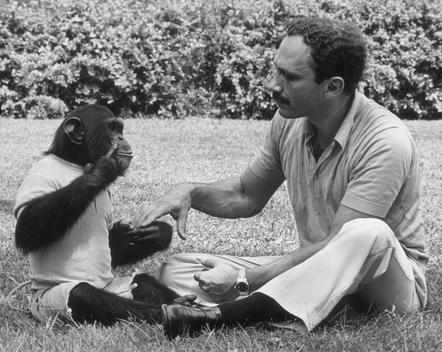
\includegraphics[height=2.7cm]{01-introduction/figs_and_tables/nim.jpg}}%
\vspace{7pt}
\noindent Nim Chimpsky (November 19, 1973 – March 10, 2000) was a chimpanzee who was the subject of an extended study of animal language acquisition at Columbia University, led by Herbert S. Terrace, as a challenge to Chomsky's thesis that full-fledged language use was innate only to humans. This quote is the Nim's longest recorded sentence.
 %, when translated from sign language
 }
\end{center}


\afterpage{\blankpage}





%%  now we can start with the real thing
% \cleardoublepage
\pagestyle{headings}
\pagenumbering{arabic}

%%     The main reason we used to split the document in parts, was to compile only the relevant chapters... 
\mainmatter
% !TEX root = ../thesis_main.tex
\chapter{Introduction}
%%%%%%%%%%%%%%%%%%%%%%%%%%%%%%%%%%%%%%%%%%%%%%%%%%%%%%
%  OPENING
%%%%%%%%%%%%%%%%%%%%%%%%%%%%%%%%%%%%%%%%%%%%%%%%%%%%%%
Humans can effortlessly learn about new concepts and solve complex problems from limited, noisy or inconsistent observations and routinely make successful generalizations based on them, yet it remains a key challenge for machines to learn from such imperfect supervision. Most of today's success of data-driven machine learning systems depends on the availability of a massive amount of high-quality labeled data and in many cases.

% detour to human learning
In the context of human learning, the argument of learning with imperfect supervision has been advanced under the name ``\emph{poverty of the stimulus}'', proposed by \citet{chomsky1980rules}. It suggests that human children can learn something as complex as a natural language from the limited inputs of variable quality and need no evidence for much of the knowledge they bring to the learning process. 
% how to explain human learning considering POS?
To explain this, some researchers postulate the innateness of some knowledge.
Along with this line, Chomsky noted~\citep{chomsky1980rules}:
\begin{quote}
    ``\emph{My own suspicion is that a central part of what we call “learning” is actually better understood as the growth of cognitive structures along an internally directed course under the triggering and partially shaping effect of the environment.}''
\end{quote}

% back to machine learning
Like humans, machines are confronted with the intriguing problem of the poverty of stimulus in learning and knowledge acquisition, although capturing such human-level learning abilities, given imperfect supervision, in machines remains a fundamental challenge in many domains~\citep{lake2017building}. 
%
% pos in machines and the necessity of {data-driven + innately primed} learning 
In machine learning, a similar discussion has been put forward on how learning algorithms can deal with the problem of \emph{poverty of stimulus}. It has been argued that a learner that makes no prior assumptions has no rational basis for generalizing over unseen instances~\citep{Mitchell:1997:ML}, which implies ``the futility of unbiased learning''.\footnote{There has been a long discussion between rationalists and empiricists. Here, we just want to draw a connection between the process of learning in humans and machines in terms of \emph{poverty of stimulus}.}

%%%%%%%%%%%%%%%%%%%%%%%%%%%%%%%%%%%%%%%%%%%%%%%%%%%%%%
%  FIRST PART OF THE TITLE: "LEARNING WITH IMPERFECT SUPERVISION [...]"
%%%%%%%%%%%%%%%%%%%%%%%%%%%%%%%%%%%%%%%%%%%%%%%%%%%%%%
% What is important supervising and why learning with imperfect supervision?

The performance of machine learning models is often strongly correlated with the amount of available labeled data:
the more data you have, the more accurate your model will be~\citep{halevy2009unreasonable,sun2017revisiting}.  
However, in many real-world applications, large-scaled high-quality training data is not available.
This highlights the increasing need for building models with the ability to learn complex tasks with \emph{imperfect supervision}. 
In this thesis, we use ``\emph{imperfect supervision}'' as an umbrella term covering a variety of situations where the learning process is based on imperfect training examples~\citep{zhou2018brief}.


%%%%%%%%%%%%%%%%%%%%%%%%%%%%%%%%%%%%%%%%%%%%%%%%%%%%%%
%  SECOND PART OF THE TITLE: "[...] FOR LANGUAGE UNDERSTANDING"
%%%%%%%%%%%%%%%%%%%%%%%%%%%%%%%%%%%%%%%%%%%%%%%%%%%%%%
% why language understanding?
We focus on language understanding and reasoning as a pivotal problem in artificial intelligence.  Understanding language is one of the extraordinary cognitive abilities of humans. 
There have been several attempts to study whether non-human animals can acquire human language~\citep{pepperberg2017animal}, like Project Nim\footnote{\url{https://nl.wikipedia.org/wiki/Project_Nim}}, a research project that was mounted in the 1970s to determine whether a chimpanzee, named Nim Chimpsky, raised in close contact with humans could develop a limited language. 

Regardless of the fact that at the end of the project Nim was using language to communicate or simply going through a bag of tricks to get things, it was much more limited compared to what a human child can develop in the early years. 
%
This indicates that achieving human-level understanding and generation of language would not be an easy goal for machines either and despite the good performance on benchmark datasets, machines are nowhere near the skill of humans at language understanding and reasoning.

Here, in this thesis, we concentrate on language understanding and reasoning in more principled ways to improve the learning process than ad-hoc and domain or task-specific tricks and investigate our ideas on a wide range of sequence modeling and language understanding tasks.

%%%%%%%%%%%%%%%%%%%%%%%%%%%%%%%%%%%%%%%%%%%%%%%%%%%%%%
%  CLOSING THE INTRO SECTION IF THE INTRODUCTION CHAPTER!
%%%%%%%%%%%%%%%%%%%%%%%%%%%%%%%%%%%%%%%%%%%%%%%%%%%%%%
\medskip
% Although machine learning has made a lot of progress on mastering its practical shortcomings, e.g., modern neural networks overcoming the limitations of the early perceptrons~\citep{minsky69perceptrons}, some of the fundamental limitations, e.g., Chomsky's Poverty of Stimulus, remain.

The main problem we study in this thesis is the poverty of stimulus for learning algorithms and to overcome this problem, we focus on  i) \emph{employing the prior knowledge}, ii) \emph{augmenting data and meta-learning how to better use the data}, and iii) \emph{introducing inductive biases to learning algorithms}, all to improve the learning process. We believe these approaches are great ways to move toward better machine learning systems that are able to generalize over observed imperfect supervision signals and as \citet{Mitchell80theneed} states in his paper:
\begin{quote}
``\emph{If biases and initial knowledge are at the heart of the ability to generalize beyond observed data, then efforts to study machine learning must focus on the combined use of prior knowledge, biases, and observation in guiding the learning process. It would be wise to make the biases and their use in controlling learning just as explicit as past research has made their observations and use.}''
\end{quote}

There are many domains and applications that suffer from the lack of a large amount of high quality labeled data. We believe building machine learning systems that can learn with imperfect supervision can be considered as a part of the bigger effort to democratize AI by making it dramatically easier to extend AI-powered systems to those domains with limited or noisy data.


\section{Problem Description and Research Questions}
Curating a large amount of high quality labeled training data has become the primary bottleneck in developing new methods and applications in machine learning~\citep{Ratner:2016}. 
% high-level ideas to deal with a lack of data
In practice, to deal with data scarcity in many tasks and applications, we can use higher-level approaches to provide supervision signals for training learning algorithms. 
% a list of alternative approaches
This can be done for instance by:
\begin{itemize}
\setlength\itemsep{0em}
\item 
Using distant, or heuristic supervision~\citep{Deriu2016:SemEval,Severyn:2015:SemEval, Dehghani:2016:SIGIR, dehghani:2018:ICLR, Dehghani:2017:nips_metalearn, Ratner:2016,Rekatsinas:2017,Varma:2017};
%
\item
Using incidental signals that exist in the data and the environment independently of the tasks and they are co-related to the target tasks~\citep{roth2017incidental}; 
%
\item
Using indirect supervision, like providing supervision by specifying constraints that should hold over the output space~\citep{stewart2017label, clarke2010driving};
%
\item
Applying bootstrapping, self-supervised feature learning, and data augmentation to make statistically efficient reuse of available data~\citep{cubuk2018autoaugment, dosovitskiy2016discriminative,donahue2016adversarial};
%
\item
Using transfer learning to generalize knowledge across domains and tasks~\citep{Ruder:2019};
%
\item
Using active learning and response-based supervision in which the model receives feedback from interacting with an environment~\citep{clarke2010driving,riezler2014response};
%
\item
Introducing a form of structured prior knowledge~\citep{Dehghani:CIKM2016:long,Dehghani:2016:ICTIR};
%
\item
Zero/one/few-shot learning~\citep{vinyals2016matching,finn2017model,snell2017prototypical,socher2013zero};
%
\item
Exploiting noisy and inaccurate labels~\citep{Vahdat:2017, Lee:2013,Hinton:2015,Brodley:1999,reed2014training, Patrini:2016, patrini2016loss,malach2017decoupling};
%
\item
Injecting inductive biases into algorithms to generalize better on unobserved data~\citep{cohen2016group, cohen2016steerable, Dehghani:ICLR:2019}.
\end{itemize}

In general supervised learning scenario, each training example, which is used as the supervision signal, consist of a \emph{feature vector} (also called data instance) and a \emph{label}. However, in many domains and applications, there is an imperfection in the supervision signal. Here, in this thesis, we focus on two main problems: dealing with \emph{noisy} training data and dealing with \emph{limited} training data. 
We formulate the main research question that is addressed in this thesis as follows:
\resq{main}

Based on the above terminology, i.e., features versus label and noisy versus limited, we can presume different types of imperfections in the supervision signal. In each part of this thesis, we target one or some of these types and proposed ideas that can improve the learning process with whit that type of imperfection in supervision. 

Figure~\ref{fig:thesis_parts} summarizes the different types of imperfection of the supervision that we consider in each part of this thesis.
\begin{figure}[t]
    \centering
    \begin{subfigure}[b]{0.32\textwidth}
    \centering
        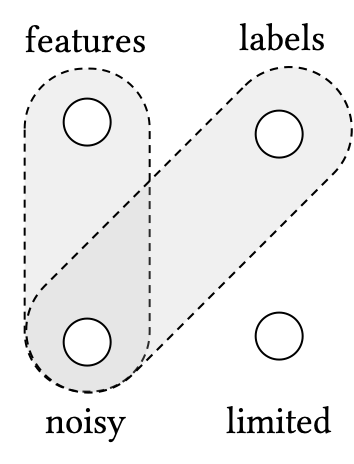
\includegraphics[width=0.55\linewidth]{01-introduction/figs_and_tables/fig_p1.png}
        \caption{\label{fig:p1}Part I}
    \end{subfigure}
        ~ 
    \begin{subfigure}[b]{0.32\textwidth}
    \centering
        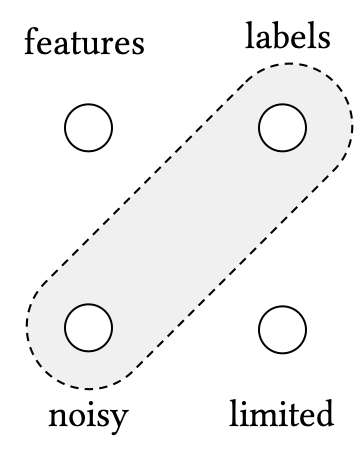
\includegraphics[width=0.55\linewidth]{01-introduction/figs_and_tables/fig_p2.png}
        \caption{\label{fig:p2}Part II}
    \end{subfigure}
        ~ 
    \begin{subfigure}[b]{0.32\textwidth}
    \centering
        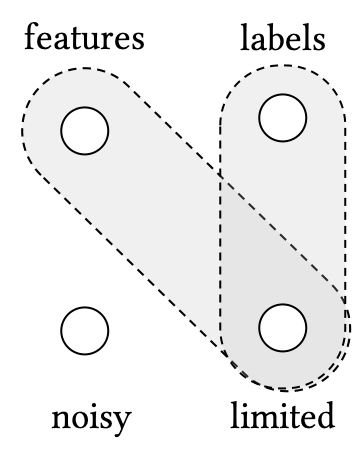
\includegraphics[width=0.55\linewidth]{01-introduction/figs_and_tables/fig_p3.png}
        \caption{\label{fig:p3}Part III}
    \end{subfigure}
\caption{\label{fig:thesis_parts}Different types of imperfection in the supervision that we deal with in each part of this thesis.}
\end{figure}

In Part~\ref{part1} of the thesis, we address the problem of noisy features. We propose robust models that can deal with non-relevant terms in relevant documents when modeling the notion of relevance in the context of relevance feedback tasks for document ranking. We also propose models that are capable of detecting and ignoring the unstable features that change over time when learning representations from data that evolves over time, as noisy factors in the data. We also partly address the problems of noisy labels by modeling the relevance in pseudo-relevance feedback tasks for document ranking, where top-k ranked documents in a retrieval run are assumed as relevant documents, while this assumption does not hold for all cases.

The proposed models in Part~\ref{part1} organized around the idea of exploring how the structure of the data can be incorporated as prior knowledge to learn representations that are more robust against noise and changes in the data during the time. 
The following research question is the main question is central to Part~\ref{part1} of the thesis:
\resq{p1}


In Part~\ref{part2} of the thesis, we target the problem of noisy or weak labels. We study how we can develop neural networks that can learn from weakly annotated training examples with the ability to go beyond the imperfection of the weak labels. We study different architectural choices and objective functions for neural ranking models to find a more noise tolerant model when learning from pseudo-labels.  We also introduce ideas that meta-learn the fidelity of weakly annotated labels and modulate the learning process based on the fidelity scores of weakly labeled examples. In fact, in this part, we make assumptions in the act of observing the data, like how to select the data based on the fidelity of data points, which is also a form of incorporating knowledge and biases.
In this part, we address the following research question:
\resq{p2}


In Part~\ref{part3}, we deal with the problem of limited labeled data, for instance, in the context of bAbI reasoning tasks with 1k training examples where the tasks are complex and training data is limited. We also study the cases where we have a lot of labeled examples, but with limited coverage, which can be seen as the limitation in the diversity of feature vectors. For instance in the context of algorithmic tasks, with the intention of assessing the ability of models on length generalization, we have plenty of training data but the distribution of sample's length in training is different from the test set. 
In this part, we investigate the idea of injecting some inductive biases\footnote{Inductive biases are ``any biases for choosing one generalization over another, other than strict consistency with the observed training samples.'' as defined by~\citet{Mitchell80theneed}. We elaborate on this at the beginning of Part~\ref{part3}.} into models in order to encode modeling assumptions that help the models to be more data efficient and generalize better.
The main research question that is addressed in Part~\ref{part3} is:
\resq{p3}


\subsection{Language Understanding and Sequence Modeling Tasks}
We study our research questions in the context of sequence modeling and natural language understanding, generation, and reasoning tasks. In the course of this thesis, we cover a wide range of tasks, including:
\begin{itemize}
\item 
Assessing relevance for ranking (Chapter~\ref{chap:2}, \ref{chap:4}; \ref{chap:5}), 
%
\item 
(Pseudo)-relevance feedback for document ranking(Chapter~\ref{chap:2});
%
\item 
Machine Translation (Chapter~\ref{chap:5});
%
\item 
Natural language reasoning ---bAbI tasks~\citep{weston2015towards} (Chapter~\ref{chap:5});
%
\item 
Broad context language modeling~\citep{paperno2016lambada} (Chapter~\ref{chap:5});
%
\item 
Contextual suggestion and recommendation~\citep{hashemioverview} (Chapter~\ref{chap:3});
%
\item 
Open-domain question answering~\citep{dunn2017searchqa, dhingra2017quasar} (Chapter~\ref{chap:5});
%
\item 
Modeling hierarchical structure in natural language ---subject-verb agreement task~\citep{linzen2016assessing} (Chapter~\ref{chap:3});
%
\item 
Text classification~\citep{Hirst:2014} (Chapter~\ref{chap:3});
%
\item 
Sentiment analysis~\citep{rosenthal2017semeval, Nakov:2016, rosenthal:2015} (Chapter~\ref{chap:5}); 
%
\item 
Learning to execute computer programs~\citep{ZS14} (Chapter~\ref{chap:5}); 
%
\item 
Algorithmic problems, like arithmetic and sequence memorization tasks ~\citep{neural_gpu} (Chapter~\ref{chap:5});
\end{itemize}

Besides the challenges of learning from imperfect supervision in many of these tasks, some of them are difficult tasks that, for instance, require learning rich representations, or capturing complex underlying relations, or detecting and understanding abstract concepts and reasoning about them.
%
Although we mainly focus on sequence modeling and language-related tasks and evaluate our proposed ideas on these tasks, many of the proposed algorithms in this thesis have no strong tie to language and can be easily extended to other domains like computer vision.
%

In the next section, we present an overview of the thesis and introduce the structure of the content and summarize different chapters in each part of the thesis.

\section{Thesis Overview}
This thesis consists of the introductory matter, followed by five main
chapters that are divided into three parts that are described in the previous section. Finally, it closes off with the Conclusions and Bibliography. 

\subsection*{PART I: \titleof{p1}}
In this part, we explore how taking the general structured of the data into account can help to estimate representations that capture only the significant features when the data is noisy and highly variant over time. We break our discussions in this part of the thesis into two chapters:

\subsubsection*{Chapter 2: \titleof{c2}}
In this chapter, we address the following research question:
\resq{c2}
We introduce \emph{\swlms} (\acswlm)~\citep{Dehghani:2016:SIGIR} to learn a representation for a set of textual entities, where this representation captures all, and only, the \textit{significant} shared features from these entities.  \acswlm adjusts the weights of features to decrease the weight of noisy terms that are either well explained by all the entities, i.e., too general or only explained by a specific entity in the set, i.e., too specific, which eventually results in having the significant features left in the model.  
We employ \acswlm in two language understanding tasks: the feedback problem in document ranking~\citep{Dehghani:CIKM2016:long, Dehghani:CIKM2016:short}, and group profiling in content personalization and recommendation tasks~\citep{Dehghani:2016:CHIIR,Dehghani2016:trec}. We show how \acswlm is remarkably robust against noisy features like non-relevant terms in relevant documents in the feedback task. 

\subsubsection*{Chapter 3: \titleof{c3}}
In this chapter, we address the following research question:
\resq{c3}
We extend \emph{\swlms} to hierarchically structured data and introduce \emph{\hswlms} (\achswlm)~\citep{Dehghani:2016:ICTIR, Dehghani:2016:CLEF} which is an iterative approach that learns representations for hierarchical entities that are highly separable as \acswlm removes the features that are well explained by either the ancestors (general features) or individual descendants (specific features). In this chapter, we discuss what makes separability a desirable property for classifiers and show how obtaining this property increases the robustness of representations against the structural changes in the data during the time.

\subsection*{PART II: \titleof{p2}}
In this part, we study how we can supervise machine learning systems by labeling training data programmatically instead of labeling by hand and discuss how to design neural networks that learn to go beyond the imperfection in the weakly annotated data. We break this into two chapters:

\subsubsection*{Chapter 4: \titleof{c4}}
In this chapter, we address the following research question:
\resq{c4}
In this chapter, we propose to train a neural ranking model using weak labels that are obtained automatically without human annotators or any external resources (e.g., click data). We train a set of simple yet effective neural ranking models and study their effectiveness under various learning scenarios, i.e., point-wise and pair-wise, different objective functions, and using different input representations~\citep{Dehghani:2017:SIGIR}. We also discuss how privacy preserving approaches can benefit from models that are capable of learning from weak signals, where instead of labels from the original sensitive training data a noisy version is provided~\citep{dehghani:2017:neuir}.

\subsubsection*{Chapter 5: \titleof{c5}}
In this chapter, we focus on the following research question:
\resq{c5}

In this chapter we introduce \emph{Learning with Controlled Weak Supervision (\cws)} and \emph{Fidelity Weighted Learning (\fwl)}, two semi-supervised approaches for training neural networks, where we have a large set of data with weak labels and a small amount of data with true labels. 
%
In \cws we train two neural networks in a meta-learning setup: a \tnet, the learner, and a \cnet, the meta-learner.  The \tnet is optimized to perform a given task and is trained using a large set of unlabeled data that are weakly annotated. We propose to control the magnitude of the gradient updates to the \tnet using the scores provided by the second \cnet, which is trained on a small amount of supervised data. Thus we avoid that the weight updates computed from noisy labels harm the quality of the \tnet model.

\fwl is a student-teacher approach in which we modulate the parameter updates to a \emph{student} network (trained on the task we care about) on a per-sample basis according to the posterior confidence of its label-quality estimated by a \emph{teacher} (who has access to the high-quality labels).  

\subsection*{PART III: \titleof{p3}}
In this part, we discuss injecting inductive biases into learning algorithms as a way to help them to come up with more generalizable solutions when they are provided with limited observations. We further discuss how we can improve the generalization of Transformers, the self-attentive feed-forward networks for sequence modeling, by introducing a recurrent inductive bias into their architecture.

\subsubsection*{Chapter 6: \titleof{c6}}
In this chapter, we address the following research question:
\resq{c6}
We introduced Universal Transformer~\citep{Dehghani:ICLR:2019}, a self-attentive concurrent-recurrent sequence model, which is an extension of the Transformer model~\citep{vaswani2017attention}. The Universal Transformer introduces recurrence in depth by repeatedly modifying a series of vector representations for each position of the sequence in parallel, by combining information from different positions using self-attention and applying a recurrent transition function across all time steps. 
In the simplest form, a Universal Transformer with a fixed number of iterations is almost equivalent to a multi-layer Transformer with tied parameters across all its layers. By sharing weights, we can save massively on the number of parameters that we are training and fewer parameters means that we learn faster with fewer data points.  We show that the elegant idea of introducing recurrence in depth enables the Universal Transformer to extrapolate from training data much better on a range of algorithmic and language understanding tasks~\citep{Dehghani:ICLR:2019, Dehghani:2019:WSDM}.

\bigskip
While the three parts of the thesis offer a complete story aligned with the goal of \emph{improving the learning process by incorporating prior knowledge, introducing right biases, and making best use of the observations from the data}, they can be read independently. 
Each of the chapters of the thesis also has their own independent research questions, proposed ideas, and take home messages, but we recommend reading them with the order they appeared in the parts.


\section{Origins}
Next, we present the origins of each chapter in terms of the papers they are based on.
\begin{itemize}
    \setlength{\itemindent}{-28pt}
    \item[]\textbf{Part I:} \emph{\titleof{p1}}
%  
        \begin{itemize}
            \setlength{\itemindent}{-33pt}
            \item[]\textbf{Chapter 2:} \emph{\titleof{c2}}
            \begin{itemize}[label=\textbullet] 
                \item \bibentry{Dehghani:CIKM2016:long}.
                \item \bibentry{Dehghani:2016:CHIIR}.
                \item \bibentry{Dehghani2016:trec}.
                \item \bibentry{Dehghani:2016:SIGIR} (SIGIR Doctoral Consortium Award).
            \end{itemize}
            
            {\footnotesize{MD designed the models, implemented the algorithms, ran the experiments, and did most of the writing. HA helped with the implementation and experiments. JK and DH helped with designing the model. HA, JK, DH, and MM contributed to the writing.}\medskip}
            
    
            \item[]\textbf{Chapter 3:} \emph{\titleof{c3}}
            \begin{itemize}[label=\textbullet] 
                \item \bibentry{Dehghani:2016:ICTIR} (Best Paper Award).
                \item \bibentry{Dehghani:2016:CLEF} (Best Paper Honorable Mention).
            \end{itemize}
            {\footnotesize{MD designed the models, implemented the algorithms, ran the experiments, and did most of the writing. HA helped with the implementation and experiments. JK helped with designing the model. HA, JK, and MM contributed to the the writing.}\medskip}
        \end{itemize}
%  
% \end{itemize}
% \begin{itemize}
% \setlength{\itemindent}{10pt}
    \item[] \textbf{Part II:} \emph{\titleof{p2}}
%  
        \begin{itemize}
            \setlength{\itemindent}{-33pt}
            \item[] \textbf{Chapter 4:} \emph{\titleof{c4}}
            \begin{itemize}[label=\textbullet] 
                \item \bibentry{Dehghani:2017:SIGIR}.
                \item \bibentry{dehghani:2017:neuir}.
                \item \bibentry{Dehghani2017:CIKM}.
            \end{itemize}
            {\footnotesize{MD designed the models, implemented the algorithms, ran the experiments, and did most of the writing. 
            SR and HZ helped with designing the models. SR helped with the implementation. HZ, HA, AS, SR, and JK helped with designing the experiments. EA and PF mentored the (internship) project. HZ, HA, JK, BC, MdR, SR, AS, and PF helped with writing.}\medskip}
                        
            \item[] \textbf{Chapter 5:} \emph{\titleof{c5}}
            \begin{itemize}[label=\textbullet] 
                \item \bibentry{dehghani:2018:ICLR}.
                \item \bibentry{Dehghani:2017:nips_metalearn}.
                \item \bibentry{Dehghani:2017avoiding}.
            \end{itemize}
            {\footnotesize{MD designed the models, implemented the algorithms, ran the experiments, and did most of the writing. 
            AM helped with designing the models. AM, SG, JK, and AS helped with designing the experiments. AM, SG, AS, SR, JK, and BS helped with writing.}\medskip}
        \end{itemize}
%   
% \end{itemize}
% \begin{itemize}
% \setlength{\itemindent}{10pt}
    \item[] \textbf{Part III:} \emph{\titleof{p3}}
%  
        \begin{itemize}
            \setlength{\itemindent}{-33pt}
            \item[] \textbf{Chapter 6:} \emph{\titleof{c6}}
            \begin{itemize}[label=\textbullet] 
                \item \bibentry{Dehghani:ICLR:2019}.
                \item \bibentry{Dehghani:2019:WSDM}.
            \end{itemize}
        \end{itemize}
        {\footnotesize{MD co-designed the core model (first paper) with SG, and MD extend the model (second paper). MD implemented the algorithms, ran all the experiments, and helped the writing. SG and OV mentored the (internship) project. SG did most of the writing. OV, JU, and LK helped with designing the model and designing the experiments. OV, JU, LK, HA, JK, and MdR helped with the writing.}\medskip}
%
\end{itemize}

The thesis also indirectly builds on the following papers (listed in reverse chronological order):
%  
\begin{itemize}
    \item \bibentry{Dehghani:2019:ICLR-LLD}.
    \item \bibentry{Dehghani:2018:SIGIRForum}.
    \item \bibentry{Zamani:2018:CIKM}.
    \item \bibentry{Azarbonyad:2018:TKDE}.
    \item \bibentry{Dehghani:2018:LND4IR}.
    \item \bibentry{Zamani:2018:LND4IR}.
    \item \bibentry{Azarbonyad:2017:CIKM}.
    \item \bibentry{Kenter:2017:NN4IR}.
    \item \bibentry{Dehghani:2017:ICTIR}.
    \item \bibentry{Dehghani:2017:CHIIR}.
    \item \bibentry{Dehghani:2017:CHIIR}.
    \item \bibentry{Azarbonyad:2017:ECIR}.
    \item \bibentry{Dehghani:2016:DIR}.
    \item \bibentry{Dehghani:CIKM2016:short}.
    \item \bibentry{Quiroz:2016:CLEF}.
    \item \bibentry{Hashemi:2015:TREC}.
    \item \bibentry{Dehghani:2015:DIR}.
    \item \bibentry{Tabrizi:2015:ICTIR}.
    \item \bibentry{Azarbonyad:2015:CLEF}.
    \item \bibentry{Azarbonyad:2015:SIGIR}.
    \item \bibentry{Dehghani:2015:ECIR}.
    \item \bibentry{Olieman:2014:ERD}
\end{itemize}
% !TEX root = ../thesis-main.tex
% \part{Learning Representations Using the Structure of the Data as Prior Knowledge}
\part{\titleof{p1}}
\label{part1}
%

The world is structural, or at least, humans understand it in structural terms. When we learn, we either fit the new knowledge into our existing structured representations or we adjust the existing structure to better accommodate our new and the old observations~\citep{battaglia2018relational}.
%
Our brain uses \emph{hierarchies} to abstract away fine-grained differences and model different levels of associations~\citep{Ballard:2015}. Using such a structure as a prior, we automatically condense the information, which not only has the impurity removal effect, but also eliminates unnecessary details, which eventually help us to memorize, think and reason in a more efficient way.

When building intelligent machines, we need to consider that the real-world data can be complex, limited, highly variable, and noisy. However, in many cases, there is a general structure that the data follow and taking this structure into account facilitates modeling complex information, adding biases to compensate the limited availability of the data, discovering robust knowledge from the data, and learning representations that are less affected by non-essential features. 
%
In Part~\ref{part1} of this book, we address one of our research questions:
\resq{p1}

We focus on transforming the textual data into digestible representations, which is the key step for any data-oriented method~\citep{Bengio:2013}. We concern with questions surrounding how we can best learn representations for entities in the world that are precise, robust against noise, transferable over time, and interpretable by human inspection.  

In the first chapter of this part, Chapter~\ref{chap:2}, we address the following research question:
\resq{c2}

We introduce \emph{\swlms} (\acswlm)~\citep{Dehghani:2016:SIGIR} of a set of documents, that capture all, and only, the significant shared terms from these documents.  This is achieved by adjusting the weights of terms already well explained by the document collection as well as the weight of terms that are only explained by specific documents, which eventually results in having the significant terms left in the model. 
Our main contributions are the following.
We apply the resulting models to two main language understanding applications: feedback problem in information retrieval\citep{Dehghani:CIKM2016:long, Dehghani:CIKM2016:short}, and group profiling in content personalization and recommendation tasks\citep{Dehghani:2016:CHIIR,Dehghani2016:trec}. We furthered argue that \acswlm are remarkably robust representations that are insensitive to the noisy terms and at the same time interpretable by human inspection. 

Then, in the second chapter of this part, Chapter~\ref{chap:3} we get down to the following research question:
\resq{c3}

We extend \emph{\swlms} to the hierarchical structure and introduce \emph{\hswlms} (\achswlm)~\citep{Dehghani:2016:ICTIR, Dehghani:2016:CLEF} that learns representations for hierarchical entities. \achswlm iteratively sparsifies the representation of the entities by discarding features that are well explained by their ancestors, i.e., general features, as well as features that reflect the characteristics of individual descendants, i.e., specific features. This leads to representations for entities that are both vertically and horizontally separable, in terms of their position in the hierarchy. We discuss what makes separability a desirable property for classifiers and show how obtaining this property leads to time-agnostic representations, i.e.  representations that are invariant to the structural changes in the data during the time.

\medskip
We show that taking the structure and the relations in the data into account, we can effectively learn representations that are less affected by the noisy variant factors in the data. We use the learned representations to solve different language understanding tasks and observe boosts in the performance, in particular due to the robustness of the learned representations against noise.

\chapter[]{\titleof{c2}}
\label{chap:2}
%
\begin{quote}
When learning representations from the data, there are general features that are not discriminating enough and specific features that are not essential to represent the data in all the cases. Taking the structure and the relations in the data into account can help learning representations that capture only and all significant features and are less affected by the noisy factors in the data.
\end{quote}
%
\section{Introduction}
Humans instinctively know how to efficiently ``select details'' that are useful for recognition and at the same time ``abstract away'' unnecessary or noisy details.~\cite{tenenbaum2011grow, gentner1997structure, battaglia2018relational} 
This is, in fact, a survival trait, since we cannot possibly save all the detail around us in our brain. Hence, to define objects and actions, we can extract a subset from an extensive but finite set of existing features that are neither \emph{too specific}, nor \emph{too general}, but \emph{significant}. In many cases, this is done by analyzing inheritance (is-a) and composition (has-a) relationships between concepts, entities, and actions~\citep{goodwin2005reasoning, botvinick2008hierarchical}. 

Inspired by that, in this chapter, we explore ideas to address one of our research questions:
\resq{c2}

We present our ideas and discussions in the context of language understanding tasks, in particular modeling textual entities for information retrieval applications. As the modeling approach, we estimate unigram language model, or so-called  ``bag of words'' model, to represent an entity, like a person, organization, category, etc, given a set of texts connected to the entity.  In fact, we assume that the textual documents associated with an entity are samples drawn from the distribution of a model that represents the entity and then estimate the model given these samples.

More specifically, we introduce \textsl{\swlms}\ (\acswlm)~\cite{Dehghani:CIKM2016:long, Dehghani:2016:CHIIR, Dehghani2016:trec} as a family of models aim at learning representations for an entity, given a set of documents associated with the entity, so that \emph{all, and only}, the significant shared terms are captured in the models. This makes these models to be not only distinctive but also supported by all the documents in the set. In short, this is achieved by adjusting the weights of terms already well explained by the all the existing documents in the collection as well as the weight of terms that are only explained by a specific document in the set, which eventually results in having the significant terms left in the model. 

\definecolor{sp}{HTML}{e92085}
\definecolor{ge}{HTML}{20b7e9}
\definecolor{re}{HTML}{b7e920}
    
\newcommand\gauss[2]{1/(#2*sqrt(20*pi))*exp(-((x-#1)^2)/(0.03*#2^0.5))} % Gauss function, parameters mu and sigma

\begin{figure}[t!]
    \centering
    \begin{tikzpicture}
    \begin{axis}[every axis plot post/.append style={
      mark=none,samples=50,smooth}, % All plots: from -2:2, 50 samples, smooth, no marks
      %grid=both,
    % xlabel style = {font=\fontsize{9}{10}\selectfont},
    % ylabel style = {font=\fontsize{9}{10}\selectfont},
    ylabel=Frequency,
    xlabel=Terms,
    xmax=0.8,
    ymax=0.5,
    width=11cm,%\textwidth,
    height=6cm, %5cm,
    xtick=\empty, 
    ytick=\empty,
    axis x line*=bottom, % no box around the plot, only x and y axis
    axis y line*=left, % the * suppresses the arrow tips
    enlargelimits=upper] % extend the axes a bit to the right and top
    
    %\addplot [fill=cyan!20, draw=none, domain=0.2:0.4] {(1/70)^x} \closedcycle;
    \addplot[mark=none,domain=0.27:0.53,
                white,
                samples=100,%
                fill = cyan!40!black!20,
                %dashed,
                pattern=north east lines,%
                pattern color=re!70!black
                ]%
                {((1/30)^(x-0.001))/2}
                 \closedcycle;
    \addplot[thick,green!20!black,domain=0:1,dashed] {\gauss{0.4}{0.4}};
    \addplot[very thick,cyan!20!black,domain=0:1]{((1/30)^(x-0.001))/2};
    \addplot[dashed] coordinates{(0.27,0)(0.27,0.4)};
    \addplot[dashed] coordinates{(0.53,0)(0.53,0.4)};
    \node[black,below] at (axis 
    cs:0.12,0.2){\small{\color{ge!60!black}{General}}};
    \node[black,below] at (axis cs:0.4,0.42){\small{\color{re!60!black}{Significant Words}}};
    \node[black,below] at (axis cs:0.7,0.2){\small{\color{sp!60!black}{Specific}}};
    % \node (One) at (axis cs:0.286,0.23) [] {}; 
    % \node (Two) at (axis cs:0.506,0.23) [] {};
    %  \pgftransformreset
    % \pgftransformyshift{.5cm}
    % \draw[decoration={
    %     text along path,
    %     text format delimiters={|}{|},
    %     text={|\fontsize{7}{8}\selectfont\color{re!50!black}|
    %     Significant Words},
    %     text align={center},
    %     },decorate] (One) to [bend left=65] (Two);
        
    \end{axis}
    % \vspace{-5pt}
    \end{tikzpicture}
    \caption{\label{fig:Luhn} Establishing a set of ``Significant Words'' based on~\citet{Luhn:1958}.}
% \vspace{-15pt}
\end{figure}


The general the idea of \acswlm is inspired by the early work of \citet{Luhn:1958}, in which he argues that to extract \textbf{significant words}, we need to avoid both common observations and rare observations. \citeauthor{Luhn:1958} assumed that frequency data can be used to measure the significance of words concerning their ability to represent a piece of text.  Considering Zipf's Law, he simply devised a counting technique for finding significant words where he specified two cut-offs based on collection frequency of terms, an upper and lower (see Figure~\ref{fig:Luhn}), to exclude non-significant words.

There have been efforts to bring this idea to estimate a more precise language model, like mixture models~\citep{Zhai:SMM:2001} and parsimonious language models~\citep{Hiemstra:2004}. These work tried to improve the raw language model by eliminating the effect of common terms from the model. However, instead of using fixed frequency cut-offs, they made use of a more advanced way to do this. \citeauthor{Hiemstra:2004} stated the following in their paper:
\begin{displayquote}

\textsl{
[\ldots] our approach bears some resemblance with early work on information retrieval by Luhn, who specifies
two word frequency cut-offs, an upper and a lower to exclude non-significant words. 
The words exceeding the upper cut-off are considered to be common and those below the lower cut-off rare, and therefore not contributing significantly to the content of the document. \ul{Unlike Luhn, we do not exclude rare words} and we do not have simple frequency cut-offs [\ldots]}

\end{displayquote} 
In a way, the idea of \acswlm completes the cycle, implementing the vision of \citeauthor{Luhn:1958}.  We introduce a meaningful translation of both \textit{specificity} and \textit{generality} against \textit{significance} in the context of learning representation for an entity given the set documents associated with it. Then we propose an effective way of estimating a model in which we learn a distribution over terms that is affected by neither the common observations nor the rare observations. 
%

While estimating \acswlm, as a distribution over terms to represent an entity given the set of documents associated with it, we cast aside terms that are not specific enough to reflect features of the entity that makes its representation distinguishable from other entities. At the same time, we abstract away from noisy factors of variation which are document specific terms that are not general enough to describe all the documents as a set representing the entity.


\subsection{Preliminaries}
~\label{chap2_preliminaries}
In Part~\ref{part1} of this book, i.e. Chapter~\ref{chap:2} and ~\ref{chap:3}, an ``entity'' can refer to a concept, a person, an organization, a category, or an ideology, where the entity is associated with a set of texts that are sequences of words. The associated texts with an entity, for instance for the aforementioned examples, can be speeches given by the person, the documents published by the organization, the text associated by instances of the category, and the set of documents describing the ideology.
%
% We also focus on learning representations that capture the \emph{notion of relevance} for applications like retrieval, where the main goal is retrieving relevant information, given a query, and classification where the main goal is to classify entities into classes based on their relevance to the underlying concepts of class labels.
%
Here, as the modeling approach, we use ``language model'' and we stick to the simplest form of language models, unigram language model, in which we assume that a word sequence is generated by generating each word independently that specifies a multinomial distribution over all the words. Thus, the probability of a sequence of words would be equal to the product of the probability of each word.  

In order to model an observed sequence of words $d$, we assume it is generated using a unigram language model $\theta$ and we would like to infer the $\theta$, i.e., estimate the probability of each word $w$ given the model, $p(w|\theta)$, based on the observed $d$. 

As an standard and simple way, we can estimate the language model using maximum likelihood estimator and find the $\hat{\theta}$ that gives the observed data the highest likelihood:
\begin{equation}
\hat{\theta} = \argmax_\theta p(d|\theta)
\end{equation}

By writing down the log-likelihood function and using the Lagrange multiplier to combine the constraint of $\sigma_{w in v}p(w|d) =1$ with the original log-likelihood function, we can get to a new unconstrained optimization problem. Then, by taking partial derivatives of this function and setting them to zero, we can obtain the solution for $\theta$ which gives each word a probability equal to its relative frequency in $d$:
\begin{equation}
    p(w|\hat{\theta} = \frac{c(w, d)}{|d|},
\end{equation}
where $c(w, d)$ is the count of word $w$ in $d$ and $|d|$ is the length of $d$ that is equal to total number of words in $d$.

Unigram language model clearly makes unrealistic assumptions about independent word occurrences in text. To address this limitation, $N-$gram language model captures some limited dependency between words and assumes the occurrence of a word depends on the proceeding $n-1$ words.  However, as the complexity of a language model increases, so does the number of parameters and we would need much more data to infer the model. Moreover, the computational cost of complex language models is also a concern for some of the large-scale retrieval or classification tasks. 
%
In information retrieval, bigram or trigram language models tend not to improve much over the unigram language model. This might be due to the data sparseness where bigram or trigram language models overfit, or the information about presence or absence of words and word frequencies may be sufficient to determine the relevance of a document while the exact word order may not be so important, unlike other language understanding tasks like machine translation or speech recognition. For machine translation, unigram language models are clearly insufficient and more sophisticated language models would be needed. 

Since a language model is a probabilistic model of text data, a direct way of evaluating a language model would be to assess how well the model fits the test data, for instance using the likelihood of the test data given a model to be evaluated, where a higher likelihood would indicate a better fit, thus a better language model.
However, fitting the data well does not necessarily imply better performance for the task at hand. To avoid this gap, here we use an indirect way of evaluating the quality of a language model by assessing the contribution of them to the retrieval or classification performance.

\subsection{Detailed Research Questions}
We break down our main research question in this chapter into three concrete research questions:
\begin{resqbox}
\begin{enumerate}
\item[\textbf{\resqname{c2.1}}] \emph{\resqcontent{c2.1}}
\item[\textbf{\resqname{c2.2}}] \emph{\resqcontent{c2.2}}
\item[\textbf{\resqname{c2.3}}] \emph{\resqcontent{c2.3}}
\end{enumerate}
\end{resqbox}
In the following sections, we will address these research questions one by one.

\section{\SWLMs}
\label{sec:swlm}
In this section, we address the first research question of this chapter: 
\resq{c2.1}

We introduce \SWLMs and describe how to estimate it. \acswlm assumes that terms in the associated documents are drawn from three models: 1.~\emph{General model}, representing common observations, 2.~\emph{Specific model}, representing partial observations, and 3.~\emph{Significant words model}. 

The significant words model is the latent model representing the essential features of the entity. The general and specific models, however, are not necessarily topic-centric models. In a way, they are supposed to represent two distributions of terms that are not considered as significant information. 

Each model is represented using a terms distribution, i.e., a unigram language model, $\theta_{sw}$, $\theta_g$, and $\theta_s$. 
We assume each term in a document in the set is generated by sampling from a mixture of these three models independently. Thus, the probability of appearance of the term $t$ in the document $d$ is as follows:
\begin{equation}
p(t|d) =  \lambda_{d,sw} p(t|\theta_{sw}) + \lambda_{d,g} p(t|\theta_g) + \lambda_{d,s} p(t|\theta_s),
\end{equation}
where $\lambda_{d,x}$ stands for $p(\theta_x|d)$ which is the probability of choosing the model $\theta_x$ given the document $d$. 

We estimate the general and specific models based on the patterns of the occurrences of terms in different documents in the set and make them fixed in the estimation process as infinitely strong priors. 
We consider the collection model, i.e. the set of all the existing documents, $\theta_C$ as an estimation for $\theta_g$:
\begin{equation}
p(t|\theta_g) = 
p(t|\theta_C) = \frac{c(t,C)}{\sum_{t' \in V} c(t',C)},
\end{equation} 
where $c(t,C)$ is the frequency of term $t$ in the collection. This way, terms that are well explained by the collection model get high probability and are considered as general terms.

Furthermore, we establish a definition for ``specificity'' with regards to our main goal which is estimating a representation for a set of documents, as being supported by part of the documents in the set but not all. We estimate $\theta_s$ to represent the probability of a term being partially observed as follows, and normalize all the probabilities to form a distribution:
\begin{equation}
p(t|\theta_s) = 
\sum_{d_i\in \mathcal{D}} 
\bigg(
p(t|\theta_{d_i}) \prod_{\substack{d_j\in \mathcal{D} \\ j \neq i}} (1-p(t|\theta_{d_j}))
\bigg),
\label{theta_s}
\end{equation}
where $P(t|\theta_{d_i}) = \nicefrac{c(t,d_i)}{\sum_{t' \in d_i} c(t',d_i)}$. 
Intuitively, Equation~\ref{theta_s} considers the probability of term $t$ to be a specific as it is important in one of the document models but not others, marginalizing over all the documents in the set. This way, terms that are well explained in only one document but not others get higher probabilities and are considered as insignificant specific terms.

Having the above assumptions, the goal is to fit the log-likelihood model of generating all terms in the documents in the set to discover the term distribution of the significant words model, $\theta_{sw}$. 
Let $\mathcal{D} = \{d_1, \ldots, d_{\mathcal{D}}\}$ be the set of documents associated withe the entity we want to learn a representation for. The log-likelihood function for the entire set of documents is:
\begin{equation}
\log p(\mathcal{D}|\Upsilon) = \sum_{d \in \mathcal{D}}\sum_{t \in V} c(t,d) \log \big(\sum_{x\in\{sw,g,s\}}\lambda_{d,x} p(t|\theta_x)\big),
\end{equation}
where $c(t,d)$ is the frequency of the term $t$ in the document $d$, and $\Upsilon$ determines the set of all parameters that should be estimated, $\Upsilon =\{\lambda_{d,sw}, \lambda_{d,g}, \lambda_{d,s} \}_{d \in \mathcal{D}} \cup \{\theta_{sw}\}$. 

To fit our model, we estimate the parameters using the maximum likelihood (ML) estimator. Therefore, assuming that documents are represented by a multinomial distribution over the terms, we solve the following problem:
\begin{equation}
\Upsilon^* = \argmax_\Upsilon p(\mathcal{D}|\Upsilon)
\end{equation}
Assuming that $X_{d,t} = \{{sw},g,s\}$ is a hidden variable indicating which model has been used to generate the term $t$ in the document $d$, we can compute the parameters using the Expectation-Maximization (EM) algorithm. 
The stages of the EM algorithm are as follows:
\begin{description}
\item[E-Step]
\begin{equation}
p(X_{d,t} = x) = \frac{p(\theta_x|d)p(t|\theta_x)}{\sum_{x' \in \{sw,g,s\}}p(\theta_{x'}|d)p(t|\theta_{x'})}
\label{EM_e}
\end{equation}
\item[M-Step]
\begin{equation}
p(t|\theta_{sw}) = 
\frac{\sum_{d \in \mathcal{D}}c(t,d) p(X_{d,t} = r)}{\sum_{t' \in V}\sum_{d \in \mathcal{D}}c(t',d) p(X_{d,t'} = r)}
\label{EM_m1}
\end{equation}
\begin{equation}
\lambda_{d,x}  = p(\theta_x|d) = 
\frac{\sum_{t \in V}c(t,d) p(X_{d,t} = x)}{\sum_{x' \in \{sw,g,s\}}\sum_{t \in V}c(t,d) p(X_{d,t} = x')}
\label{EM_m2}
\end{equation}
\end{description}

\input{02-part-01/chapter-02/figs_and_tables/fig_plate_diagram.tex}
Figure~\ref{fig:graphical-model} represents the plate notation of \acswlm. As it is shown, for each document the contribution of each of the three models, i.e., $\lambda_{d,x} \text{for} x \in \{sw,g,s\}$, are estimated. It can be seen that general model, $\theta_g$, and the specific model, $\theta_s$ are considered as external observations, which are involved in the estimation process as infinitely strong priors. 

In the next section, We employ \acswlm in different applications in order to assess its effectiveness on modeling an entity given a set of documents that are associated with the entity. We evaluate \acswlm on relevance feedback in the retrieval task, where we need to model the set of relevant documents or top-ranked documents in the initial retrieved results and use this model to expand the user's query to improve the retrieval performance by shrinking the vocabulary gap between query and relevant documents. Furthermore, we use \acswlm as a group profiling approach in the task of contextual suggestion to model a preferences of a group of people and augment user profiles with the profiles of implicit or explicit groups they belong to.
\section{\acswlm for Relevance Feedback}
Modeling and assessing ``relevance" is the main goal in information retrieval and search that requires understanding users' queries, documents, and the relation between them.
One of the key factors affecting search quality is the fact that user queries are ultra-short statements of their complex information needs. Query expansion has been proven to be an effective technique to bring agreement between user information need and relevant documents~\citep{Harman:2009}. 
Taking feedback information into account is a common approach for enriching the representation of queries and consequently improving retrieval performance. 

In the True Relevance Feedback (TRF), given a query and a set of judged documents, either explicitly assessed by the user or implicitly inferred from user behavior, the system tries to enrich the query representation to improve the performance of the retrieval. However, feedback information is not available in most practical settings. An alternate approach is the Pseudo Relevance Feedback (PRF), also called blind relevance feedback, which uses the top-ranked documents in the initial retrieved results for the feedback.

The main goal of feedback systems in retrieval task is to make use of feedback documents to estimate a more accurate query model representing the notion of relevance.
%
However, although documents in the feedback set contain relevant information, there is always also non-relevant information. For instance, in PRF, some documents in the feedback set might be non-relevant, or in TRF, some documents, despite the fact that they are relevant, may contain off-topic information and act like poison pills~\citep{Terra:2005} by hurting the performance of feedback systems.  
Such non-relevant information can distract the feedback model by adding bad expansion terms, leading to \emph{topic drift}~\citep{Macdonald:2007,He:2009:ECIR}.  
It has been shown that based on this observation, existing feedback systems are able to improve the performance of the retrieval, if feedback documents are not only relevant, but also have a dedicated interest in the topic~\citep{He:2009:ECIR}.


Given that, taking advantage of feedback documents requires a robust and effective method to prevent topic drift caused by \emph{accidental}, non-relevant terms brought in by broader topic or multiple topics documents in the feedback set. 

\textsl{\swlm} seems a great fit to this situation as it models the the set of feedback documents by capturing the essential terms representing a \emph{mutual notion of relevance}, i.e.\ a representation of characteristic terms which are supported by all the feedback documents.

\input{02-part-01/chapter-02/figs_and_tables/fig_prf_example.tex}
Figure~\ref{fig:prf_eg} shows an example of estimating language models from the set of top seven relevant documents retrieved for topic $374$, ``Nobel prize winners'', of the TREC Robust04 test collection.  
Terms in each list are selected from top 50 terms of the models estimated after stop word removal. 
Standard-LM is the language model estimated using MLE considering feedback documents as a single document. 
SMM is the language model estimated using mixture model~\citep{Zhai:SMM:2001}, one of the most powerful feedback approaches, which generally tries to remove background terms from the feedback model.

%
General-LM denotes the probability of terms to be common based on their overall occurrence in the collection and Specific-LM determines the probability of terms to be specific in the feedback set, i.e being frequent in one of the feedback documents but not others. 
The way General-LM and Specific-LM are estimated has been discussed in detail in Section~\ref{sec:swlm}. 
And the last model in the figure is \acswlm, which is the extracted latent model with regards to General-LM and Specific-LM, using \swlms.

As can be seen, considering feedback documents as a mixture of feedback model and collection model, mixture model~\citep{Zhai:SMM:2001} penalizes some general terms like ``time'' and ``year'' by decreasing their probabilities. However, since some frequent words in the feedback set are not frequent in the whole collection, their probabilities are boosted, like ``Palestinian'' and ``Arafat'', while they are not good indicators for the whole feedback set. The point is although these terms are frequently observed, they only occur in some feedback documents not most of them, which means that they are in fact ``specific'' terms, not significant terms.
By estimating both general model and specific model and taking them into consideration, \acswlm tries to control the contribution of each feedback document in the feedback model, based on its merit, and prevent the estimated model to be affected by indistinct or off-topic terms, resulting in a significant model that reflects the notion of relevance.

Here, we are going to address our second research question of this chapter: 
\resq{c2.2}

We explain how to estimate \acswlm for a set of feedback documents and discuss its effectiveness in this task along with a set of analisys and ablation studies.

\subsection{Language Models for Feedback}
Language modeling is usually used to represent the user query by estimating a query language model, $\theta_q$, based on maximum likelihood estimation:
$p(t|\theta_q)=\nicefrac{c(t,q)}{|q|}$, 
where $c(t,q)$ is the frequency of term $t$ in $q$ and $|q|$ is the total number of terms in the query.
Then, usually having the smoothed language model of documents~\citep{Zhai:2001}, the KL-divergence retrieval model~\citep{Lafferty:2001} is employed to score documents based on the negative KL-divergence between the estimated language models of the query and each document document:
\begin{equation}
Score(d,q) = -D(\theta_q||\theta_d)
\label{scoring}
\end{equation}
In order to elaborate the problem of vocabulary difference between the query and relevant documents, and overcome the lack of agreement on the notion of relevance between the user and the system, a feedback language model, $\theta_\mathcal{F}$,  is estimated using the set of feedback documents and then this model is employed to expand the query. A common approach for expanding the query is interpolating $\theta_\mathcal{F}$ with the original query model~\cite{Zhai:SMM:2001,Abdul-jaleel:2004}:
\begin{equation}
p(t|\theta_{q}') = (1-\alpha)p(t|\theta_q)+\alpha p(t|\theta_\mathcal{F}),
\label{interpolation}
\end{equation}
where $\alpha$ controls the amount of feedback. Thereafter the expanded query model is used in Equation~\ref{scoring} for ranking the documents.

The main goal of feedback methods is to estimate an effective feedback model, $\theta_\mathcal{F}$, from the set of feedback documents. 
We can use \swlms to represent feedback documents. In this context, the significant words are in fact words that are reflecting the notion of relevance. We use the approach described in ~\ref{sec:swlm}, where we take the $\theta_{sw}$ as the $\theta_\mathcal{F}$  and use it in Equation~\ref{interpolation} for expanding the query. 

\input{02-part-01/chapter-02/figs_and_tables/fig_plate_diagram_rswlm.tex}
\subsection{Regularized \acswlm}
Using the original \swlms for estimating the feedback model, the original query model has not been considered for estimating the feedback model. Thus, in case of having a few relevant documents in the feedback set for a query, the model could be distracted by non-relevant information and converge to a local optimum point.

To cope with this problem, and avoid degradation in the performance, a solution is to involve information from the original query~\citep{Harman:1992}. Inspired by the work by \citet{Tao:2006}, we modify the estimation process of \acswlm and estimate \RSWLMs (\acrswlm) by incorporating the extra knowledge from the query model. We define a prior parameter and employ maximum a posteriori to fit the model to feedback documents and solve the following problem:
\begin{equation}
\Upsilon^* \coloneqq \argmax_\Upsilon p(\mathcal{F}|\Upsilon)P(\Upsilon)
\end{equation}
%Since Dirichlet distribution is a conjugate prior for multinomial distributions, we only need to slightly modify the M-step for reestimating $\theta_{sw}$ in the EM algorithm to incorporate this prior.
We define the a conjugate Dirichlet prior on $\theta_{sw}$ as follows:
\begin{equation}
p(\theta_{sw}) \varpropto \prod_{t \in V} p(t|\theta_{sw})^{\beta p(t|\theta_q)},
\end{equation}
where $\beta p(t|\theta_q)$ is the parameter of the Dirichlet distribution which in fact performs as the additional pseudo-count for  $t$ to push the model $\theta_{sw}$ to assign a higher probability to term $t$ as it has a high probability in $\theta_q$. 

Generally speaking, this adds a bias in the estimation process to bend the feedback model toward the original query model. 
Here, the value of $\beta$ controls the amount of this bias. 
Taking the conjugate prior into account, we conduct the MAP estimation by updating Equation~\ref{EM_m1} in the EM algorithm as follows:
\begin{equation}
p(t|\theta_{sw}) = 
\frac{\sum_{d \in \mathcal{F}}c(t,d) p(X_{d,t} = sw) + \beta p(t|\theta_q) }{\sum_{t' \in V}\sum_{d \in \mathcal{F}}c(t',d) p(X_{d,t'} = sw) + \beta}
\label{EM_m1_new}
\end{equation}
So, by modifying the EM algorithm, we consider our observation from the query model as a pseudo-document which makes the feedback model become more rigid. 

Similar to the approach in \citep{Tao:2006}, we initialize $\beta$ with a large value, and then dynamically decrease its value in each EM iteration until the point that we have equal contributions of the original query and the feedback documents. 
Figure~\ref{fig:graphical_model_rswlm} represents the plate notation of \rswlms. 

As it is shown, for each document the contribution of each of three models, $\lambda$s, are estimated. It can be seen that general model, $\theta_g$, and specific model, $\theta_s$ are considered as external observations, which are involved in the estimation process as infinitely strong priors. It is noteworthy that fixing these parameters also helps to decrease the number of local maximums. As it is illustrated in the diagram, $\beta$ plays the role of regularizing parameter. 

Establishing a model consisting only the significant words using the fixed cut-offs based on frequency of terms, as was originally proposed by~\citet{Luhn:1958}, runs the risk of leaving good expansion terms out, especially trimming the model toward specific terms may lead to the loss of discriminative relevant terms that can have a high impact on retrieval effectiveness. \acswlm enables us to reduce this risk as estimating specific language model using Equation~\ref{theta_s}, makes a meaningful translation of specificity against the significance, which empowers our estimation process to retain the significant terms that are globally infrequent, but well supported by the feedback documents.

%---------------------------------------
\subsection{Experimental Setup}
\label{sec:dataset}
%---------------------------------------
\input{02-part-01/chapter-02/figs_and_tables/table_prf_dataset.tex}
In this section, we describe the test collections used in our experiments as well as the settings of our experiments. 
We use the Robust04, WT10G, and GOV2 test collections, which are different in terms of both size and genre of documents. 
Information about each collection is summarized in Table~\ref{tbl_dataset}.

We have employed the Lemur toolkit and Indri\footnote{\url{http://www.lemurproject.org/}} search engine to carry out our experiments. We have implemented \acswlm and \acrswlm in Lemur project framework. 
In all our experiments, we only use the ``title'' field of the TREC topics as queries. 
We have used the Porter stemmer for stemming all queries and document's terms and removed stopwords using the standard InQuery stopword list. 
We have used the KL-Divergence model~\citep{Lafferty:2001}, with Dirichlet smoothing~\citep{Zhai:2001} as the retrieval model in all of the experiments, including initial retrievals as well as feedback runs.
We set the Dirichlet smoothing prior to $1,000$.  In the feedback runs, for each collection and each method, we have done full grid search and tuned three main parameters: the value of the feedback interpolation coefficient, the number of feedback documents, and the number of expansion terms, by dividing the queries into three folds and conducting 3-fold cross-validation with the same split for folding in all the experiments.  Also we have tuned the hyperparameters of each method during the cross validation.

%
The Mean Average Precision (MAP) performance measure for top $1,000$ documents is presented as the evaluation metric. 
Moreover, we report P@10 (precision at 10) for PRF and P@20 (precision at 20) for TRF as the indicators of the precision for the \emph{first} and \emph{two-first} result pages, respectively.  
To avoid the ranking effect in the evaluation of the TRF task, we have used modified freezing technique in the evaluation of the results of these experiments \citep{cirillo:1969,Harman:1992,Ruthven:2003}. In addition to the above metrics, we also report robustness index, $RI(Q)$, which is also called reliability of improvement~~\citep{Collins-Thompson:2007}. For a set of
queries $Q$, the $RI$ measure is defined as: $RI(Q) = \nicefrac{N^+ - N^-}{|Q|}$, where $N^+$ is the number of queries helped by the feedback method and $N^-$ is the number of queries hurt.

In our experiments, as the baseline methods, we have used the most popular unsupervised state-of-the-arts for the feedback task that are proposed in the language modeling framework. 
Our baseline methods are: the maximum likelihood estimation\:---\:without feedback (MLE)~\citep{Lafferty:2001}, the simple mixture model (SMM)~\citep{Zhai:SMM:2001},  the divergence minimization model (DMM)~\citep{Zhai:SMM:2001}, the relevance models (RM3 and RM4)~\citep{Abdul-jaleel:2004,Lavrenko:2001}, the regularized mixture model (RMM)~\citep{Tao:2006}, and maximum-entropy divergence minimization model (MEDMM)~\citep{Lv:2014}. 


\subsection{\acswlm for Relevance Feedback}
Now, we present the results of applying \acswlm on both true and pseudo relevance feedback tasks.

%---------------------------------------
\subsubsection{\acswlm for True Relevance Feedback}
\label{sec:RF}
%---------------------------------------
\input{02-part-01/chapter-02/figs_and_tables/table_trf.tex}
True relevance feedback is employed to expand the user query based on either the explicit ``relevant''/``non-relevant'' judgments given by the user or implicit relevancy information inferred from the user behavior during his interaction with the system, for the top-k results returned by the retrieval system. 
In our experiments, we simulated this task. We consider the set of relevant documents on the top-10 results (first page of the search engine result page) in the ranked list as the documents judged as relevant by the user to form the feedback set. In our TRF experiments, same as~\citet{Lv:2009:CIKM}, we have removed queries that have no relevant documents in their top-10 results from the test collections. Information on the number of queries used for TRF in each collection is given in Table~\ref{tbl_dataset}.

Table~\ref{tbl_rf} presents the results of different systems on the TRF task. As can be seen, \acswlm and \acrswlm are best methods in terms of MAP\@ and RI in all the collections and in terms of P@20 in the Web collections. 
Since we have used the modified freezing technique~\cite{cirillo:1969,Ruthven:2003}, in the feedback runs, almost the top 10 results are the same as the initial run, so the improvements in the P@20 metric is sort of a reflection for the precision of second 10 results (second page of SERP). 

In the TRF task, although the relevancy information of documents are available,  since documents can be multi-topic, it is still possible that the feedback mechanism selects the terms from non-relevant parts of the documents. In the Robust04, in which documents are not normally multi-topic, RM3 performs the best in terms of P@20. However, in the Web collections, which is more likely to contain multi-topic documents (partially relevant), \acswlm, by controlling the effect of individual documents on the feedback model, significantly outperforms all the baselines.

Unlike the results in Table~\ref{tbl_prf}, in which \acrswlm performs better than \acswlm in terms of all metrics, in TRF, \acswlm presents higher performance in terms of P@20. This might be due to the fact that in TRF, there is less noise and consequently less need to lead the feedback model toward the original query model. On the other hand, since \acrswlm has no bias to the original query, it has the opportunity to retrieve some documents that are relevant but terms of the original query do not occur in them frequently. 

\medskip
Here, we presented the results of \acswlm  and \acrswlm  in the tasks of PRF and TRF compared to the baseline methods.
We show that the new models are more effective than all previous methods, and also illustrated how they control the contribution of feedback documents in the feedback model based on their merit.
Recall that our approach takes a considerable risk by removing specific terms that are the most powerful retrieval cues if relevant, making the feedback task a critical experiment in distinguishing relevant and non-relevant terms. 
%
These results provide strong support for effectiveness of \swlms, and the general intuitions on the importance of building accurate models of relevance underlying them.


\input{02-part-01/chapter-02/figs_and_tables/table_prf.tex}
%---------------------------------------
\subsubsection{\acswlm for Pseudo Relevance Feedback}
\label{sec:PRF}
%---------------------------------------
Pseudo relevance feedback aims to expand the query to improve the performance of retrieval having no information about the judgments. In PRF, the underlying assumption is that the initial retrieval yields the relevant documents which can be used to refine the query. Thus, assuming the top-ranked documents $\mathcal{F} = \{d_1, \ldots ,d_{\mathcal{F}}\}$ from the initial run as relevant, the feedback model $\theta_{\mathcal{F}}$ is estimated and used for the query expansion.  
Table~\ref{tbl_prf} presents the results of employing \swlms, \rswlms as the feedback model as well as baseline methods on the task of PRF\@. 
As can be seen, \acrswlm significantly outperforms \emph{all} the baselines in terms of MAP, in WT10G and GOV2 collections, that are noisy Web collections.\footnote{Note that we only indicate when (R)\acswlm is significantly better than all baseline methods, they are always significantly better than the non-expansion MLE baseline.} Furthermore, it has the highest reliability of improvements in terms of Robustness Index in all the collections.
In the PRF task, \acrswlm works better than \acswlm as it guides the estimator of the feedback model toward the query model and prevents it to be distracted by the noises of non-relevant documents.

Although it has been shown that PRF always improves the average performance of retrieval \citep{Harman:2009}, under some parameter settings, for some topics it decreases the average precision.  This is due to the fact that there might be some non-relevant documents in the feedback set containing non-relevant terms resulting to the topic drift in the extracted feedback model~\cite{He:2009:ECIR,He:2009:CIKM,Carpineto:2012}. Thus, as one of the main challenging problems in PRF, it is necessary to control the contribution of different feedback documents for inclusion in the feedback model based on their merit~\citep{He:2009:ECIR} for a specific query. 

\subsection{Relevance Decomposition}
\input{02-part-01/chapter-02/figs_and_tables/plot_prf_lambdas.tex}
\Swlms empower our proposed feedback method to dynamically determine the quality of each document.
In Figure~\ref{fig:lambdas}, as a sample, we take top-100 documents as the feedback set and illustrate the average contribution of each of the significant words, general, and specific models in this documents, according to the $\lambda$s learned in the \rswlms. 

It is an interesting observation that in all the collections the trend of the change in the contribution of three models is similar. 
In most cases, as the ranking goes down, the contribution of the significant words model decreases, which is in accordance with the relevance probability of documents based on their ranking.  However, this decay is slower in the Robust04 dataset compared to WT10G and GOV2 datasets.  This is likely because that Robust04 contains newswire articles, which are typically high-quality text data with little noise, in contrast to WT10G and GOV2 which are web collections containing a more heterogeneous set of documents.  
%This could mean that lower ranked documents for Robust still having a considerable number of terms in common with top-ranked documents.

Another interesting observation is that in all the collections we see that the top ranked documents are more likely to contain specific non-related terms than general non-related terms. In other words, as the rank of the document increases, the part of the document which is non-relevant becomes more general. 
%
One assumption would be that the retrieval models may tend to rank documents with specific non-related terms higher than documents with general non-related terms.  However, traditional retrieval models like KL-Divergence do not differ scores of documents based on their non-relevant part. Another hypothesis would be that, the specificity or generality of the non-related parts of documents is a matter of their length. For example, long documents are more probable to have specific non-related terms than short documents. We investigated the length of the retrieved documents based on their ranking in our experiments and, although the retrieval models in general might have some length bias~\citep{Losada:2008}, we observed no strong correlation between length and the ranking in our runs.

Based on the observation from Figure~\ref{fig:lambdas}, we can conclude that the relevant component captured by the significant words dominates the ranking (as would be hoped and expected) and after that the specific component, and lastly the general component (in line with term weighting methods in the ranking models). These observations support that the proposed model is indeed more accurately modeling relevance than standard IR models.
More generally, this analysis shows the analytic potential of the proposed model, for example to analyse the ranking of partially relevant or multi-topic documents, based on the generality or specificity of the subtopics involved, which we will defer to future work.

%if the non-relevant part is about a specific topic, the relevant part is stronger in terms of relevancy compared to the case that the non-relevant part is general. 
%In other words, on average, in multi-topic documents, the relevant part has a stronger focus on the query and they are ranked higher, while in broad topic documents, the relevant part has less interest to the query.
%We are going to investigate this observation in more details in our future works.

%---------------------------------------
\subsection{Robustness Against Noise}
\label{sec:robustness}
%---------------------------------------
This section present analysis resulted from experiments designed to study the robustness of our proposed feedback approach.

\input{02-part-01/chapter-02/figs_and_tables/plot_prf_divergence.tex}
%\subsection{Robustness in PRF: Divergence from Relevance}
\subsubsection{Divergence from Relevance}
\label{sec:DfR}
%---------------------------------------
As an experiment that we have designed to investigate the ability of the each feedback method to deal with noise in the PRF task, using top retrieved results, we measure the divergence of the estimated pseudo relevance feedback models, $\theta_{\mathcal{F}}^{prf}$, from the estimated true relevance models, $\theta_{\mathcal{F}}^{trf}$, that use only those documents from the top retrieved that are explicitly annotated as relevant.
%
%
In fact, investigate that how much a feedback method is able to estimate model from a mixture of relevant and non-relevant documents that are similar to the model estimated using only the relevant part. 
To this end, we assume that $\theta_{\mathcal{F}}^{trf}$, is a model affected by least amount of noise and calculate the JS-Divergence of $\theta_{\mathcal{F}}^{prf}$ and  $\theta_{\mathcal{F}}^{trf}$ for all the approaches and 
to avoid the effect of the size of the models on the value of divergence, we take top 500 terms of each model as the fixed length representative of the model. 

Figure~\ref{fig:div} shows the divergence of $\theta_{\mathcal{F}}^{prf}$ and  $\theta_{\mathcal{F}}^{trf}$ for different groups of queries with different ratio of relevant documents in top-10 documents, on all collections. As it is expected, in the queries that have a few documents in the top-10 documents are relevant, the divergence is high and two models getting to be the same when all top-10 documents are relevant. 
In Web collections, convergence of $\theta_{\mathcal{F}}^{prf}$ and  $\theta_{\mathcal{F}}^{trf}$ are slower due to the fact that web documents are more noisy and it can be said that usually non-relevant retrieved documents are farther from relevant retrieved documents, compared to Robust04 dataset. 
According to the plots in Figure~\ref{fig:div}, in all collections, \acswlm  and \acrswlm  have the least divergence in all the ratios. It means that our proposed models are more robust against being distracted by non-relevant documents. 
An interesting observation is that in all the collections, the behavior of \acswlm  and \acrswlm  are almost the same when at least half of the documents are relevant. In other words, we do not need regularization if at least half of the documents are of interest to the query's topic, either completely or partially.

\input{02-part-01/chapter-02/figs_and_tables/table_prf_robustness.tex}
%---------------------------------------
\subsubsection{Dealing with Poison Pills}
\label{sec:pp}
%---------------------------------------
Although it has been shown that on average, the overall performance will be improved after feedback~\citep{Harman:2009,He:2009:ECIR}, for some topics, employing some documents may decrease the average precision of the initial run. 
As we discussed, in the PRF, it could be due to the fact that the harming feedback documents are not relevant. However, this also could happen in the RF. This is because although the harming feedback document is relevant, there could be only a subset of it containing relevant information. So, adding off-topic terms from this document to the query results in loosing the retrieval performance. These relevant documents that hurt the performance of retrieval after feedback are called ``poison pills''~\citep{Harman:2009,Warren:2004,Terra:2005,Dehghani:CIKM2016:short}.

\citet{Terra:2005} studied the effect of the poison pills. They used a single relevant document for feedback with several systems to find documents that make the precision drop in all systems. They showed that more than $5\%$ of all relevant documents perform poorly and in one third of all topics there exists at least one bad relevant document which can decrease the performance of the retrieval after relevance feedback.

We have investigated this effect in the multiple feedback documents experiments. In these experiments, for each topic with more than ten relevant documents, we add relevant documents one by one, based on their ranking in the initial run, to the feedback set and keep the track of the change in the performance of the feedback run after adding each relevant document to the feedback set compared to the feedback run without its presence in the feedback set.  
%
\input{02-part-01/chapter-02/figs_and_tables/plot_prf_poisonpill.tex}
%

To evaluate the robustness of different systems against bad relevant documents, we define a variant of \emph{Robustness Index ($RI$)}~\citep{Collins-Thompson:2007} to be applicable in the document level instead of topic level. For a set of
relevant documents,$D_r$, the $RI$ measure is defined as: $ RI(D_r)= \nicefrac{N_r^+ -  N_r^-}{|D_r|}$ where $N_r^+$ and $N_r^-$ denote number of relevant documents which adding them to the feedback set, based on the above setting, respectively helps or hurts the performance of the feedback run in terms of AP, compared to the case of not including them. $|D_r|$ is total number of tested relevant documents. The higher the value of $RI(D_r)$ is, the more the method is robust against poison pills. Table~\ref{tbl_pp} presents the $RI(D_r)$ of different systems on different datasets. As can be seen, both systems based on \swlms  are strongly robust against the effect of bad relevant documents in all datasets. 

Furthermore, we have looked into the results of experiments in all the collections and extracted the set of poison pills, i.e. relevant documents that adding them to the feedback set decreases the  performance of feedback in \emph{all} the baseline systems. 
Overal, we found $118$ poison pills and we observed that the performance of \acrswlm  in these situations always has the least drop and in $92\%$ of the cases, it provides the best average precision after adding the poison pill. 

As it is discussed by~\citet{Terra:2005}, poison pills are usually relevant documents which have either a broad topic, or several topics. In these situations, employing \swlms  enables the feedback system to control the contribution of these documents and prevents their specific or general terms affect the feedback model. Figure~\ref{fig:pp} shows how using \swlm  empowers the feedback system to deal with the poison pills. In this figure, the performance of different systems in topic $374$ on Robust04 dataset are illustrated. As can be seen, adding the seventh relevant document to the feedback set leads to a substantial decrement in the performance of the feedback in all the systems. The query is ``Nobel prize winners" and the seventh document is about one of the Nobel peace prize winners, Yasser Arafat, but at the end, it has a discussion concerning Middle East issues, which contains some highly frequent terms that are non-relevant to the query (see Figure~\ref{fig:prf_eg}).  
However, \acrswlm  and \acswlm  are able to distinguish this document as a poison pill and by reducing its contribution to the feedback model, i.e. learning a low value for $\lambda_{d_7,sw}$, they prevent the severe drop in the feedback performance. 

So, our method inoculates the feedback model against poison pills by automatically determining whether adding a specific relevant document to the feedback set hurts the retrieval performance for a specific topic or not and controls its effect in the feedback model.


\subsubsection{Sensitivity to the Number of Feedback Documents}
\input{02-part-01/chapter-02/figs_and_tables/plot_prf_num_doc_sensitivity.tex}
In order to investigate the sensitivity of our proposed method to the number of documents in the task of PRF, which is a proxy to it sensitivity to the noisy documents in the feedback set, we set all other free parameters to the values that result in optimal average performance and  plot the performance of \acswlm  and \acrswlm  with regard to the number of documents in the feedback set in Figure~\ref{fig:sens}. As it is noticed,  both methods have acceptable robustness. 
\acswlm  is more sensitive, especially in Web collections, when low ranked documents are added, it is slightly affected by noises.  However, \acrswlm  is strongly robust and less sensitive to the number of feedback documents.

Furthermore, according to Figure~\ref{fig:sens}, the performance of both systems in all collections is the best when the number of feedback documents are around 10, which is a more or less the same observation in other feedback methods as well~\citep{Lv:2009}. Moreover, this observation is in accordance with the information from the plots in Figure~\ref{fig:lambdas}, in which the top-10 documents always possess a strong contribution of the significant words model, i.e.\ high values of $\lambda_{d,sw}$.


\section{\acswlm for Contextual Suggestion}
Context is pervasive on the modern web, due to cloud-based and mobile applications, making every information access interaction part of an eternal user session.  Effective ways to leverage this context are key to further enhancing the user experience, both in terms of better quality of results as in terms of easier ways to articulate complex information needs.  This requires both effective ways of personalization to an individual user as well as customization to a profile based on groups of users.

For group level analysis, there is a need for extracting a group profile that captures the essence of the group, separate from the sum of the profiles of its individual members. This profile should be ``specific'' enough to distinguish the preferences of the group from other groups, and in the same time, ``general'' enough to capture all shared tastes, expectations, and similarities of its members. 

Group profiling can help understand both explicit groups, like Facebook groups, and implicit groups, like groups extracted by community detection algorithms. One of the important applications of group profiling is in the contextual suggestion problem~\citep{hashemioverview}.  
Contextual suggestion is the task of searching for complex information needs that are highly dependent on both context and user interests. However, using individual preferences for contextual suggestion is not always possible. 
For example, sometimes there is a new user in the system with no historical interactions and no rich information about the preferences\footnote{Cold start problem in contextual suggestion.}, or sometimes the user is not able to determine his/her preferences explicitly. In these situations, group based contextual suggestion would be beneficial to augment the user's profile and suggest content to the user based on the preferences of the groups that the user belongs to. 

In contextual suggestion, given the information of users including their age, gender, and set of rated places or activities as the user preferences (ratings are in the range of -1 to 4), the task is to generate a list of ranked suggestions from a set of candidate attractions, by giving the user information as well as some information about the context, including location of trip, trip season, trip type, trip duration, and the type of group the person is travelling with.

We employed \acswlm for group profiling to be able to employ group information in the contextual suggestion task~\citep{Dehghani2016:trec,Dehghani:2016:CHIIR,Hashemi:2015}. We use group profiles estimated by \acswlm with respect to the different grouping criteria and investigate how group-based information helps to improve the general performance of contextual suggestion task. 

In the rest of this chapter, we address our third and last research question of this chapter: 
\resq{c2.3}

We explain how to use \acswlm as a profiling approach to represent a group of entities and use this representation to improve the quality of contextual suggestion task.

%---------------------------------------
\subsection{Experimental Setup}
\label{sec:cs_exp}
%---------------------------------------
\input{02-part-01/chapter-02/figs_and_tables/table_cs_statistics.tex.tex}
We use of the TREC 2015  contextual suggestion\footnote{\url{https://sites.google.com/site/treccontext/trec-2015}} Batch task dataset to evaluate the effectiveness of \acswlm as a profiling approach for the contextual suggestion task. The dataset contains the information from 207 users including their age, gender, and set of rated places or activities as the user preferences (rates are in the range of -1 to 4). 
The task is to generate a list of ranked suggestions from a set of candidate attractions, by giving the user information as well as some information about the context, including location of trip, trip season, trip type, tripe duration, and the type of group the person is travelling with. Based on the information in the dataset, we divide users into several groups. Groupings are based on the users information and context information. Table~\ref{tbl:stat} presents grouping criteria, the groups, and number of users in each group.

\subsection{\acswlm for Group Profiling}
\label{sec:groupprofiling}
We generate group-based rankings of suggestions based on the group profiles estimated by \acswlm to evaluate the quality of the estimated group profiles in contextual suggestion task. 
To this end, first we choose one of the grouping criteria mentioned in Table~\ref{tbl:stat} like users' age. Then we estimate a language model representing each group as its profile using \acswlm. Afterward, regarding the information of the given request, i.e.\ the user information and context information, the group which the user belongs to is selected and based on the profile of the this group as well as the language model of the candidate, we rank the suggestions.

Beside the group-based ranking, we generate a ranked list of suggestions based on the preferences of the users, regardless of their group memberships, as a baseline. To do so, a language model is estimated using the mixture of the language model representing user preferences weighted by their ratings. Then, based on the similarity of the preferences language model and the candidate language model, we rank the suggestions.

Using \acswlm, we learn the contribution of each of \emph{specific}, and \emph{general}, \emph{group} (which is in fact \emph{significant words}) models, i.e.\ $\lambda_{user,s}$, $\lambda_{user,g}$, and $\lambda_{user,sw}$. Having these parameters empowers us to efficiently combine the group-based model with the preferences-based model for content customization. To this end, we smooth the preferences-based model of the user with both the group model and the general model using JM-smoothing \citep{Zhai:2001} employing the learn parameters.

\input{02-part-01/chapter-02/figs_and_tables/plot_cs_perf.tex}
Figure~\ref{fig:Chart1} presents the performance of well as preferences\:-\:based suggestion as well as when we employ different grouping criteria for group-\:based suggestion. The combinations of preferences\:-\:based suggestion and group-\:based suggestion are also reported. 

Among the group-based strategies, suggestions based on the duration of the trip is the most effective strategy. Also age of the user and the type of the group the user travels with, are rather important while type of the trip is not so important. This could be due to the fact that most of the time, the user's interests and attractions do not change based on the type of trip which could be ``business'' or ``holiday''. 
On the other hand, combining the preferences-based suggestions with group-based suggestions in all grouping strategies leads to improvement. This means in case of incompleteness of user's profile, customizing the content based on the groups that user belongs to, implicitly fills the missing information and improves the performance of the suggestions. However, this depends on the quality of the groups profiles that should reflect significant (not general, not specific) characteristics of the groups.

\subsection{Effect of Group Granularity}
\label{sec:gg}
In the grouping stage, sometimes users can be grouped based on different levels of granularity. For example, having the age of users, discretization can be done using binning with different sizes of bin. In this section, we analyse the effect of granularity of groups, and consecutively the size of the groups with a fixed volume of train data, on the quality of group profiling.

We have selected ``age'' of users as the grouping criterion and tried different bin sizes for discretization: 5 years, 10 years, 20 years and 40 years. 
Figure~\ref{fig:Chart2} shows the quality of groups profiles on different levels of granularity and consequently on different sizes of groups in the task of contextual suggestion. 
Each point in the figure represents a group of users and its position determines its size and the performance of group-based contextual suggestion for the users within the group. Moreover the horizontal lines represent overall performance of different levels of granularity. 
As can be seen, since the number of sample users is limited fine-grained grouping leads to having smaller groups. So small number of samples affects the group profiling quality and slightly decreases the performance. While coarse-grained grouping leads to having large groups that leads to not being able to adequately customize the group profile. 

In our dataset, 10 years granularity for ``age'' has the best performance since the formed groups are big enough so that the group profiling approach is able to estimate high quality models, and they are small enough so that the group profiles are easily distinguishable which leads to a more effective customization.
\input{02-part-01/chapter-02/figs_and_tables/plot_cs_groupsize.tex}

\subsection{Effect of Rating Behaviour}
\label{sec:rb}
As we showed, using group-based information that is modeled by \acswlm helps to improve the performance of contextual suggestion. To study where does this improvement come from, we looked into the data to see in which cases adding group information helps and in which cases it is not effective. We observed that there is a correlation between the amount of improvement in contextual suggestion using group-based information and the rating behavior of users.

\input{02-part-01/chapter-02/figs_and_tables/plot_cs_gprate.tex}

Figure~\ref{fig:gprates} shows the scatter plot of the change in $p@10$ after employing group-based information based on different rating tendency.
According to the plot, group-based information works better when the users have a neutral tendency in their rating (around rate 2) and it is less likely to help when users have rather strong biases by rating attraction with high or low rates. This could be due to the fact that in case of having neutral users, we have less strong information coming from their profile and then group-based information is compensating this lack of strong signals.
\section{Related Work}
In this section, we discuss related studies to the applications that we evaluated \acswlm on, i.e, in feedback in the retrieval task and group profiling in contextual suggestion. 

\subsection{Relevance Feedback}
It has been shown that there is a limitation on providing increasingly better results for retrieval systems only based on the original query~\citep{Rijsbergen:1986}. So, it is crucial to reformulate the search request using terms that reflect the user's information need to improve the performance of the retrieval systems. 
To address this issue, automatic feedback methods for information retrieval were introduced fifty years ago~\citep{Rocchio:1971} and have been extensively studied  during past decades.
%~\citep{Rijsbergen:1981,Robertson:1976,Salton:1985,Robertson:1991,Harman:1992,Buckley:1994,Lavrenko:2001,Zhai:SMM:2001,Ruthven:2003,Tao:2006, He:2009:ECIR,Lv:2009,He:2009:CIKM,Harman:2009,Carpineto:2012,Lv:2014}. 
As the earliest relevance feedback approach in information retrieval, the Rocchio method~\citep{Rocchio:1971} has been proposed in the vector processing environments for changing the query vector to be similar to the relevant documents vectors and dissimilar to the non-relevant documents vectors. 
Later, probabilistic methods have been proposed to select expansion terms from feedback documents based on a term weighting approach~\citep{Robertson:1976,Rijsbergen:1981}. With the development of language models, several feedback approaches have been proposed in this framework to improve the query language model~\citep{Zhai:SMM:2001,Tao:2006,Lavrenko:2001,Hiemstra:2004,Lv:2014}. 
The mixture model~\citep{Zhai:SMM:2001} is one of the well-known feedback methods in the language modeling framework, which empirically performs well. The idea is to extract a discriminative language model of feedback documents by decreasing weights of the background terms. 
As an extension to this model, the regularized mixture model has been proposed by \citet{Tao:2006}, which not only involves the query model in the estimated feedback model but also has document-specific mixing coefficients to let different documents have a different amount of background terms.

In the relevance model (RM)~\citep{Abdul-jaleel:2004,Lavrenko:2001} given the query, a model is estimated as a multinomial distribution over terms that indicates the likelihood of each term given the query as the evidence, based on the occurrences of the term together with the query terms in the feedback documents.  In a comparable study conducted by~\citet{Zhai:SMM:2001}, it has been shown that RM3 as a variant of the relevance model is one of the best performing methods which is strongly robust.
Divergence minimization~\citep{Zhai:SMM:2001} tries to estimate a feedback model that is close to the language model of every feedback document but far from the collection language model as an approximation of the non-relevant language model. This method generates a highly skewed feedback model, which makes it unable to perform well. \citet{Lv:2014} proposed the maximum-entropy divergence minimization model that, by adding an entropy term, regularizes the original divergence minimization model leading to significant improvements in the performance of the original method.

The parsimonious language model~\citep{Hiemstra:2004} is one of the models employed for feedback~\citep{Meij:2008,Hiemstra:2008:TREC,Kaptein:2008:TREC}. It tries to describe the feedback model using a smaller number of parameters. Similar to the mixture model, the common words in the collection are removed from the model in the estimation process, which leads to a more lean and mean language model.  \citet{Zamani:2016a}, considering the feedback problem as a recommendation problem, made use of matrix factorization in order for predicting expansion terms in a weighted manner.

Besides the ad hoc studies, there have been some initiatives aimed at studying the problem of (pseudo-)relevance feedback in detail. In 2003, Reliable Information Access (RIA) Workshop~\citep{Harman:2009,Warren:2004} 
%,Gu:2004:RIA,Montgomery:2004,Lynam:2004:RIA,Terra:2005
was organized with the goal of understanding the contributions of both system variability factors and topic variability factors to the overall retrieval variability in feedback. 
%Later on, in 2008, the Relevance Feedback track was intended as one the TREC tracks and it has been continued for two more years. The initial goal of the TREC Relevance Feedback track was evaluating and comparing different feedback methods~\citep{Buckley:2008:TREC}. In the next years, the tasks in TREC Relevance Feedback track focused on studying what is a good document for relevance feedback and how a system can recognize a good document~\citep{Buckley:2010:TREC}. 
In addition to the Relevance Feedback track, the Robust track in TREC defined one of the goals to improve the consistency of feedback systems by focusing on the poorly performing topics~\citep{Voorhees:2003:TREC}.

%Applying feedback deteriorates the performance of retrieval in some topics, especially in pseudo relevance feedback in which the performance of the feedback run strongly depends on the quality of the top documents in the initial run~\citep{Harman:2009,Collins-Thompson:2009}. 
%,Billerbeck:2003
%On the other hand, using some documents (even relevant documents) might harm the feedback performance~\citep{Terra:2005,Lv:2009:CIKM}.  
%Hence, there are some challenges in the feedback problem like how to determine whether applying the feedback improves the performance for a specific topic, and how to measure the quality of each feedback document and how to incorporate this information in the feedback process.
%
%\citet{He:2009:CIKM} proposed to examine to which degree the feedback documents is about the topic of the query using Entropy. In other work~\citep{He:2009:ECIR} they try to detect good feedback documents in PRF by grouping documents employing features like the probability of the query terms in the feedback document, the similarity of each feedback document with other feedback documents, and closeness of expansion terms to the original query terms. 
%\citet{Lee:2008} proposed to find the dominant documents from the initial run as better documents for PRF\@. 
%\citet{Tao:2004} proposed a two-stage mixture model in which taking the query as a relevant prior, feedback documents are divided into relevant and background documents and only the documents in the relevant group are employed for updating the query model. 
%\citet{Collins-Thompson:2007} tried to model feedback uncertainty to improve the robustness. They proposed to perform sampling over the feedback documents as well as the query to generate different sets of feedback documents and several query variants. Then, combining different feedback models from alternative sets, the robustness of the feedback model can be improved.

\medskip
Arguably, the key issue in feedback is robustness in terms of being able to deal with non-relevant terms from non-relevant or partially relevant documents. \acswlm addresses the robustness problem head on. This is achieved by using the information from the collection and other feedback documents to control the contribution of documents in the feedback model regarding their merit and to avoid the selection of non-relevant expansion terms.

\subsection{Group profiling for Content Customization}
Group profiling can help understand both explicit groups, like Facebook groups, and implicit groups, like groups extracted by community detection algorithms. There is a wide range of applications for group profiling, like understanding social structures~\citep{Tang:2011}, network visualization, recommender systems~\citep{Hu:2014,Shang:2014,Amer-Yahia}, and direct marketing~\citep{Custers:2003}. 

There is various research done on the task of group profiling which, given the individual attributes and preferences, aims to find out group-level shared preferences~\cite{Senot:2011,Masthoff:2011}.
\citet{Tang:2011} presented three methods for group profiling: \emph{Aggregation}, which tries to find features that are shared by the whole group; \emph{Differentiation}, which tries to extract features that can help to differentiate one group from others; and \emph{Egocentric differentiation}, which tries to extract features that can help to differentiate members of one group from the neighbour members. In recent work, \citet{Hu:2014} proposed a deep-architecture model to learn a high level representation of group preferences.

For group recommendation,  there is research on building a model of a group by forming a linear combination of the individual models~\citep{Jameson:2007}. Some of them construct the group's preference model on the basis of individual preference models, using a notion of distance between preference models~\citep{Yu:2006}. Some approaches try to divide the group into several categories of homogeneous users and specify the preference model for each subgroup. Then they create the group model as a weighted average of the subgroup models, with the weights reflecting the importance of the subgroups~\citep{Ardissono:2003}.


\section{Conclusion} 
In this chapter, inspired by the discussion on the early work by~\citet{Luhn:1958} about \emph{significant words}, we proposed \emph{\swlms}\ (\acswlm) to estimate a representation for a set of documents that captures significant terms by avoiding the distracting effect of common observation as well as rare observation.

We showed that utilizing \acswlm as the feedback model presents promising performance on both true and pseudo relevance feedback. Analyzing the results, we indicated that the strength of \acswlm in feedback is due the fact that it is capable of controlling the contribution of feedback documents in the feedback model based on their level of relevancy which copes with the problem of topic drift in query expansion. We assessed the robustness of \acswlm in different experiments and showed that in PRF, both it has the least vulnerability against noise in the data in the form of non-relevant terms and/or non-relevant documents in feedback set.
%
We also employed \acswlm as a group profiling approach for the task of contextual suggestion, and our experimental results showed using the group representations estimated by \acswlm, we can improve the performance of content customization. 

We named our model, significant ``words'' language model in honor of \citeauthor{Luhn:1958}, however, it could be employed in non-textual environments, since in general, the idea is to extract significant ``features'' representing the shared essence of a group of entities.

% connecting chapter 2 to chapter 3:
The process of estimating \acswlm leads to a sparse model, i.e. $\theta_{sw}$ assigns zero probability to many terms that are identified as either too general or too specific for representing an entity. 
Sparsity has a central role in human episodic memory. In the human brain, sparse activities is important to separate representations as it reduces the risk that a single neuron holds representations of two overlapping memories\citep{cho2018blockchain}. In addition to human brain, for many systems, sparsity is a desirable property, for instance sparse representations are easier to interpret or more likely to posses separability which is important for collision resistance hash functions. 
In Chapter~\ref{chap:3}, we extend \acswlm to hierarchically structured entities and discuss separability as a key objective for learning the representations.
\chapter{Representational Separability for Hierarchically Structured Data}
\label{chap:3}
\section{Introduction}
Hierarchy is an effective and common way of representing information, and many domains are naturally organized in a hierarchy. Organizing data in a hierarchical structure is valuable since it determines relationships in the data at different levels of resolution and picks out different categories relevant to each of the various layers of memberships.  
Besides that, using hierarchies is an effective way of representing the information as it eases the task of \emph{comparison}, which is a critical factor in analogical reasoning. For example, the problem of deciding whether two entities are analogous can be formalized as the problem of checking the level of abstraction at which these entities are instances of the same node in a hierarchy.

Taking advantage of the structure in a hierarchy requires modeling and representing entities, taking their relationship in the hierarchy into consideration. 
There are two types of dependencies in the hierarchies: i) \emph{Horizontal dependency}, which refers to the relations of entities in the same layer.  A simple example would be the dependency between siblings which have some commonalities in terms of being descendants of the same entity. ii) \emph{Vertical dependency}, which addresses the relations between ancestors and descendants in the hierarchy. For example the relation between root and other entities. 

Due to the existence of two\:-\:dimensional dependencies between entities in the hierarchy, modeling them regardless of their relationships might result in overlapping models that are not capable of making different entities distinguishable.  Learning representations with minimal overlap is one of the requirements for collision resistance systems and when the representations are not well\:-\:separated, classification and retrieval systems are less likely to work well~\citep{Lewis:1992}. 
Thus, \emph{two\:-\:dimensional separability}, i.e.\ \emph{horizontal and vertical separability}, is one of the key requirements of hierarchical classification.

In this chapter, we focus on one of our research questions:
\begin{resqbox}
\emph{\resq{c3}}
\end{resqbox}
We introduce \hswlms, which extends the idea of \swlms to the hierarchical structure. We assume that entities, like people, organizations, concepts, and ideologies are organized in a hierarchy, and for each entity, there are textual data associated with the entity with respect to the subhierarchy under the entity, where the data is generated only at the leaves of the hierarchy. Each entity, which is a node in the hierarchy, is represented by a specific probabilistic language model.

Given the hierarchical structure and the data associated with entities in the hierarchy, \achswlm iteratively sparsifies the representation of the entities by discarding features that are well explained by their ancestors, i.e., general features, as well as features that reflect the characteristics of individual descendants, i.e., specific features. This leads to representations for entities that are both vertically and horizontally separable, in terms of their position in the hierarchy, as they capture only the significant features of entities.

\begin{figure}[!t]
\centering
\tikzset{
every tree node/.style={align=center,anchor=north}
edge from parent/.style={very thick},
%edge from parent/.style=
%{draw, edge from parent path={(\tikzparentnode.south)
%-- +(0,-8pt)
%-| (\tikzchildnode)}},
blank/.style={draw=none}}
\begin{tikzpicture}[level distance = 30pt]
% \fontsize{7}{8}\selectfont
\matrix
{
\node{\Tree
    [.All  \edge[blank]; 
    [.Status  \edge[blank];
    [.Party \edge[blank]; 
    [.Member ]]]]};
&
\node{\Tree 
    [.Parliament
        [.Government
            [.$P_1$  $M_1$ [.{\dots} ] [.{\dots} ] ]
            [.{\dots} ]
            [.{\dots} ]
%            [.$P_n$  $M_1$ [.{\dots} ] $M_n$ ]
        ]
        [.Opposition 
%            [.$P_1$  $M_1$ [.{\dots} ]  $M_m$ ]
            [.{\dots} ]
            [.{\dots} ]
            [.$P_n$  [.{\dots} ] [.{\dots} ] $M_m$ ]
        ]
    ]};\\
};
\shrink
\end{tikzpicture}
\caption{\label{fig:ParHierarchy}Hierarchical relations in parliament.}
\end{figure}
As a concrete example, consider a simple hierarchy of a multi\:-\:party parliament as shown in Figure~\ref{fig:ParHierarchy}, which determines different categories relevant to the different layers of membership in the parliament.  We can associate an individual member of parliament by her speeches, a political party by their member's speeches, the opposition by the speeches of members of opposition parties, etc. 
In order to represent a party in this hierarchy, a proper model would show common characteristics of its members\:---\:not members of other parties (\emph{horizontal} separation), and capture the party's generic characteristics\:---\:not unique aspects of the current members captured in the individual member's layer or aspects of whether the party is in government or opposition captured in the status layer (\emph{vertical} separation).

\subsection{The Importance of Representational Separability}
The concept of \emph{separability} is of crucial importance especially when the task is not just ranking a set of items, but making a boolean decision about the labels of each item in the set.
Regarding this concern, \citet{Lewis:1995} has presented the Probability Threshold Principle (PTP), as a stronger version of the Probability Ranking Principle~\citep{Robertson:1977}, for binary classification, which discusses optimizing a threshold for separating items regarding their probability of class membership. 
PTP is a principle based on the separability in the score space. However, here we discuss separability in the data representation and later in this chapter we define a \emph{\ssp} as the counterpart of PTP in the feature space.
\begin{figure}[t]
% \makebox[\linewidth][c]{
\centering
\begin{subfigure}{0.49\textwidth}
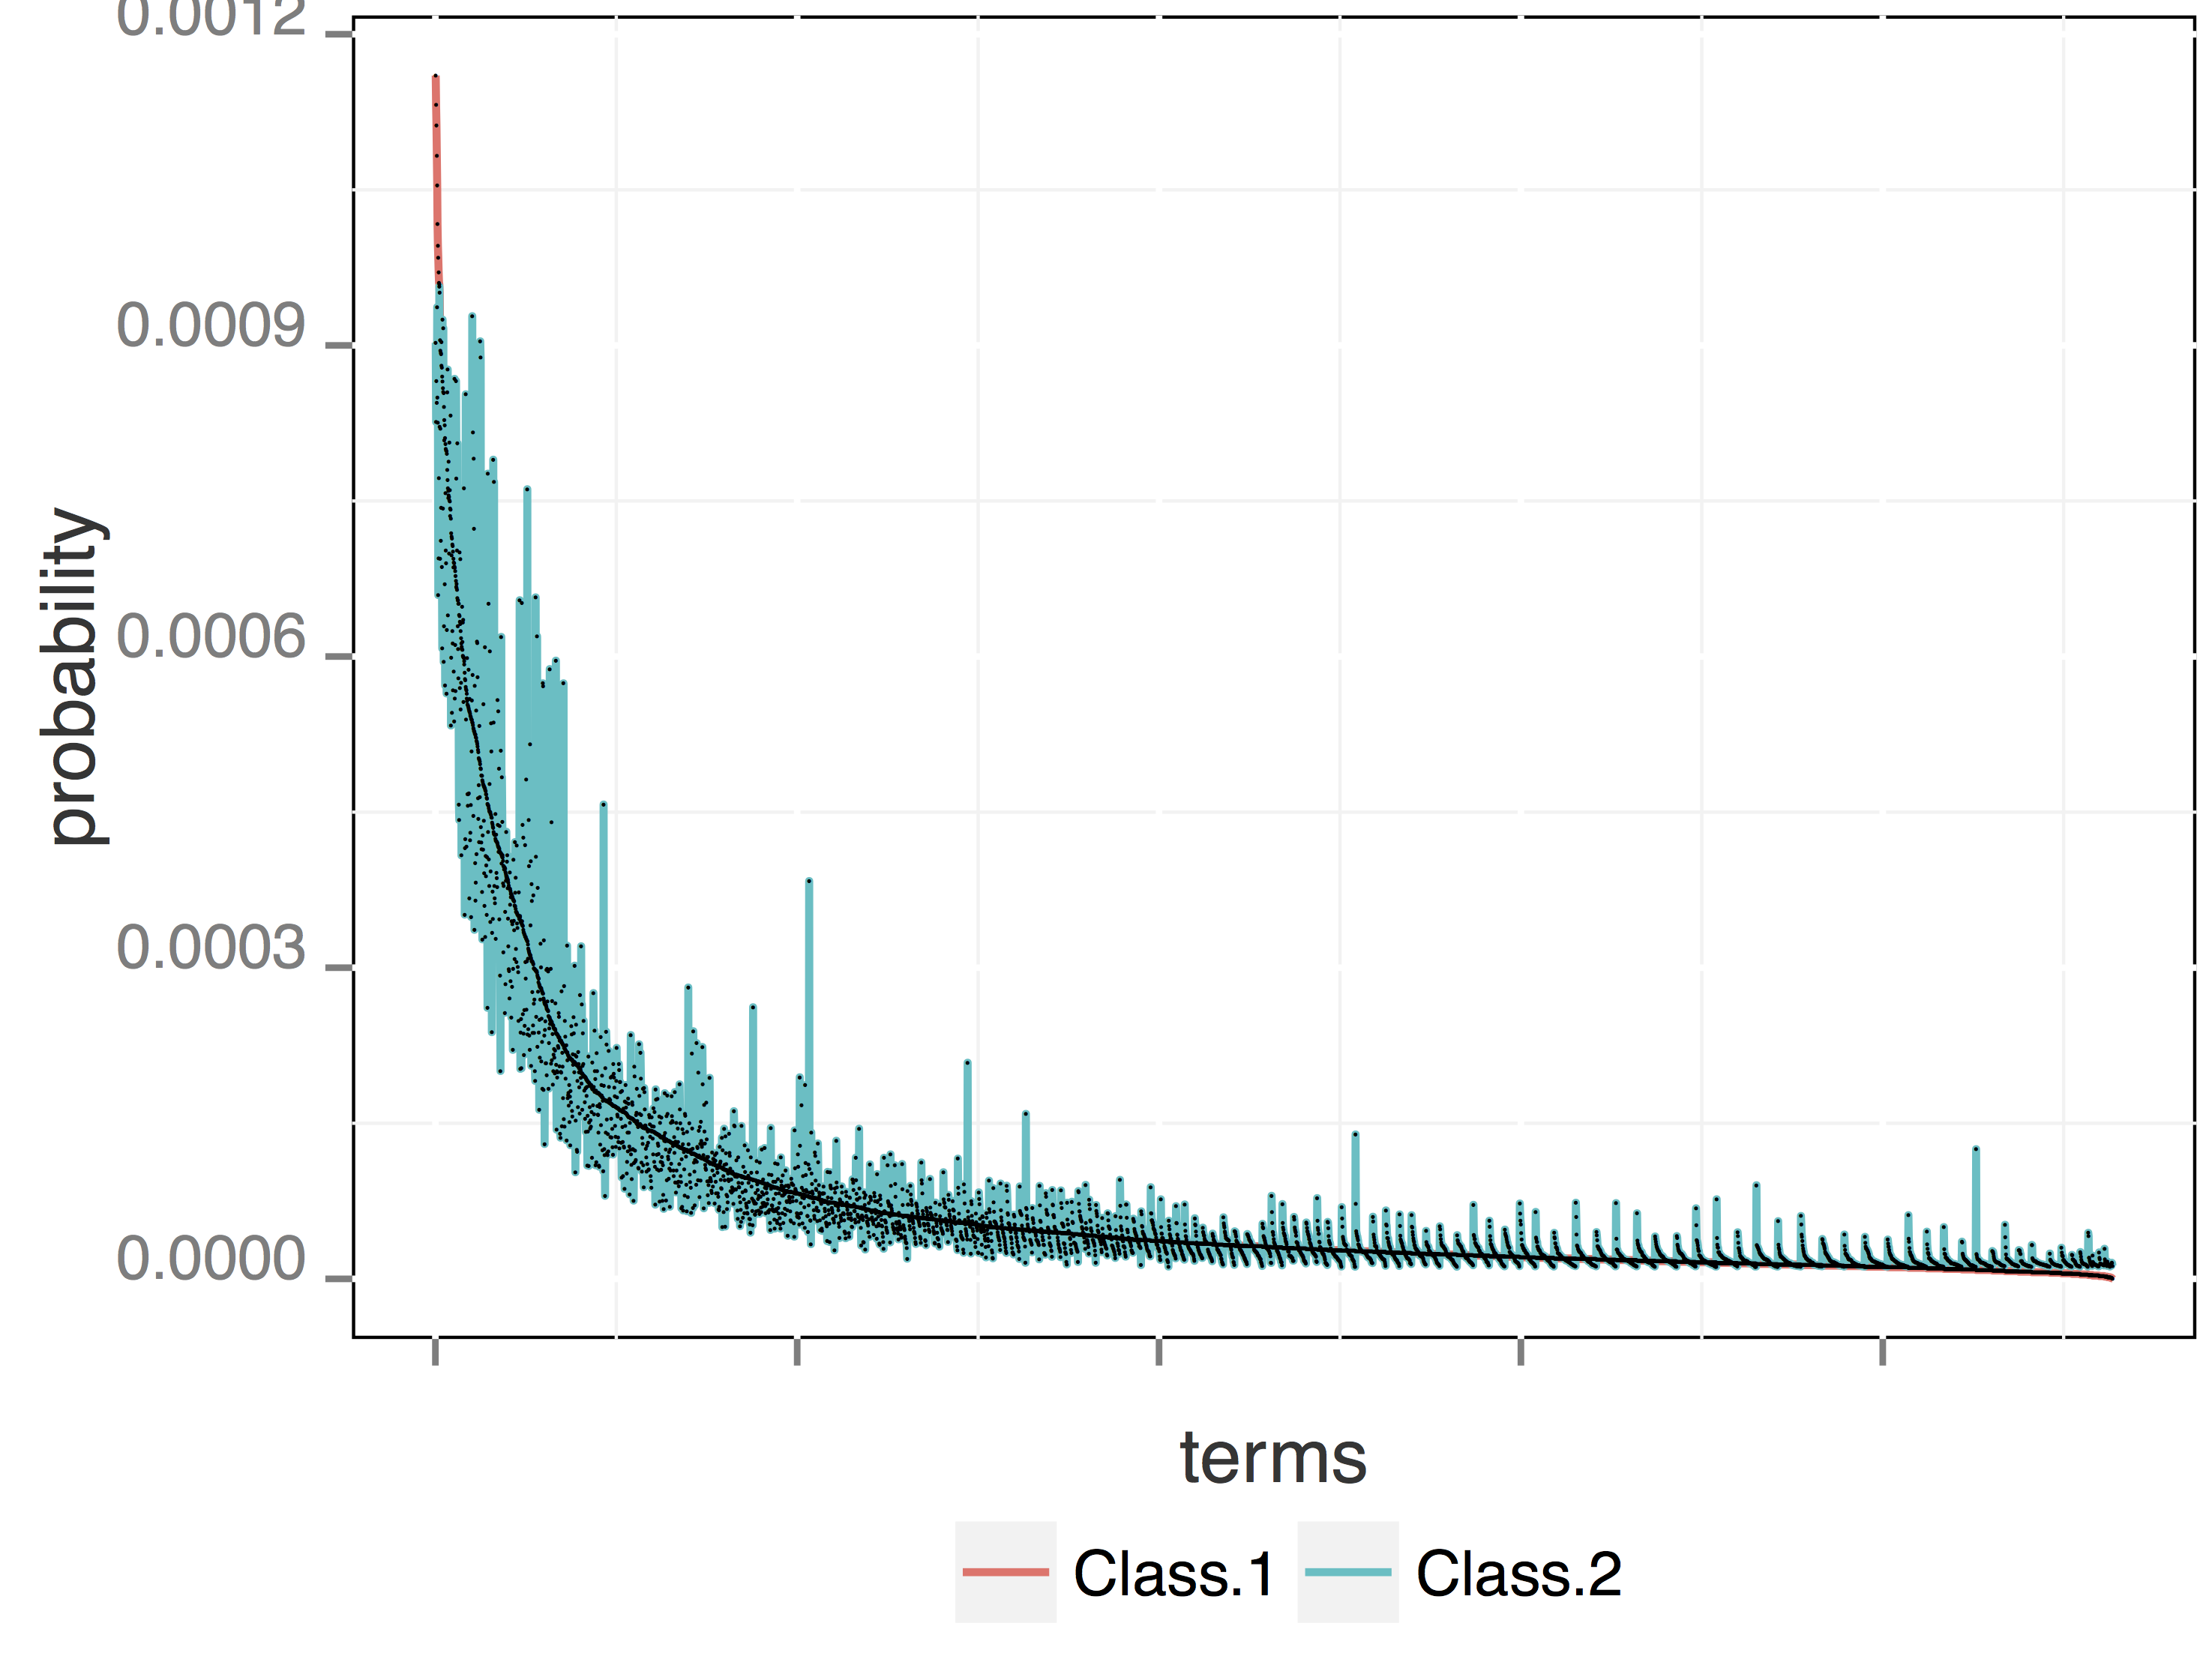
\includegraphics[width=\linewidth]{02-part-01/chapter-03/figs_and_tables/img_example-slm.png}
\caption{\label{fig:sep-slm} \scriptsize{A non-separable representation of data.}}
\end{subfigure}
\hfill
\begin{subfigure}{0.49\textwidth}
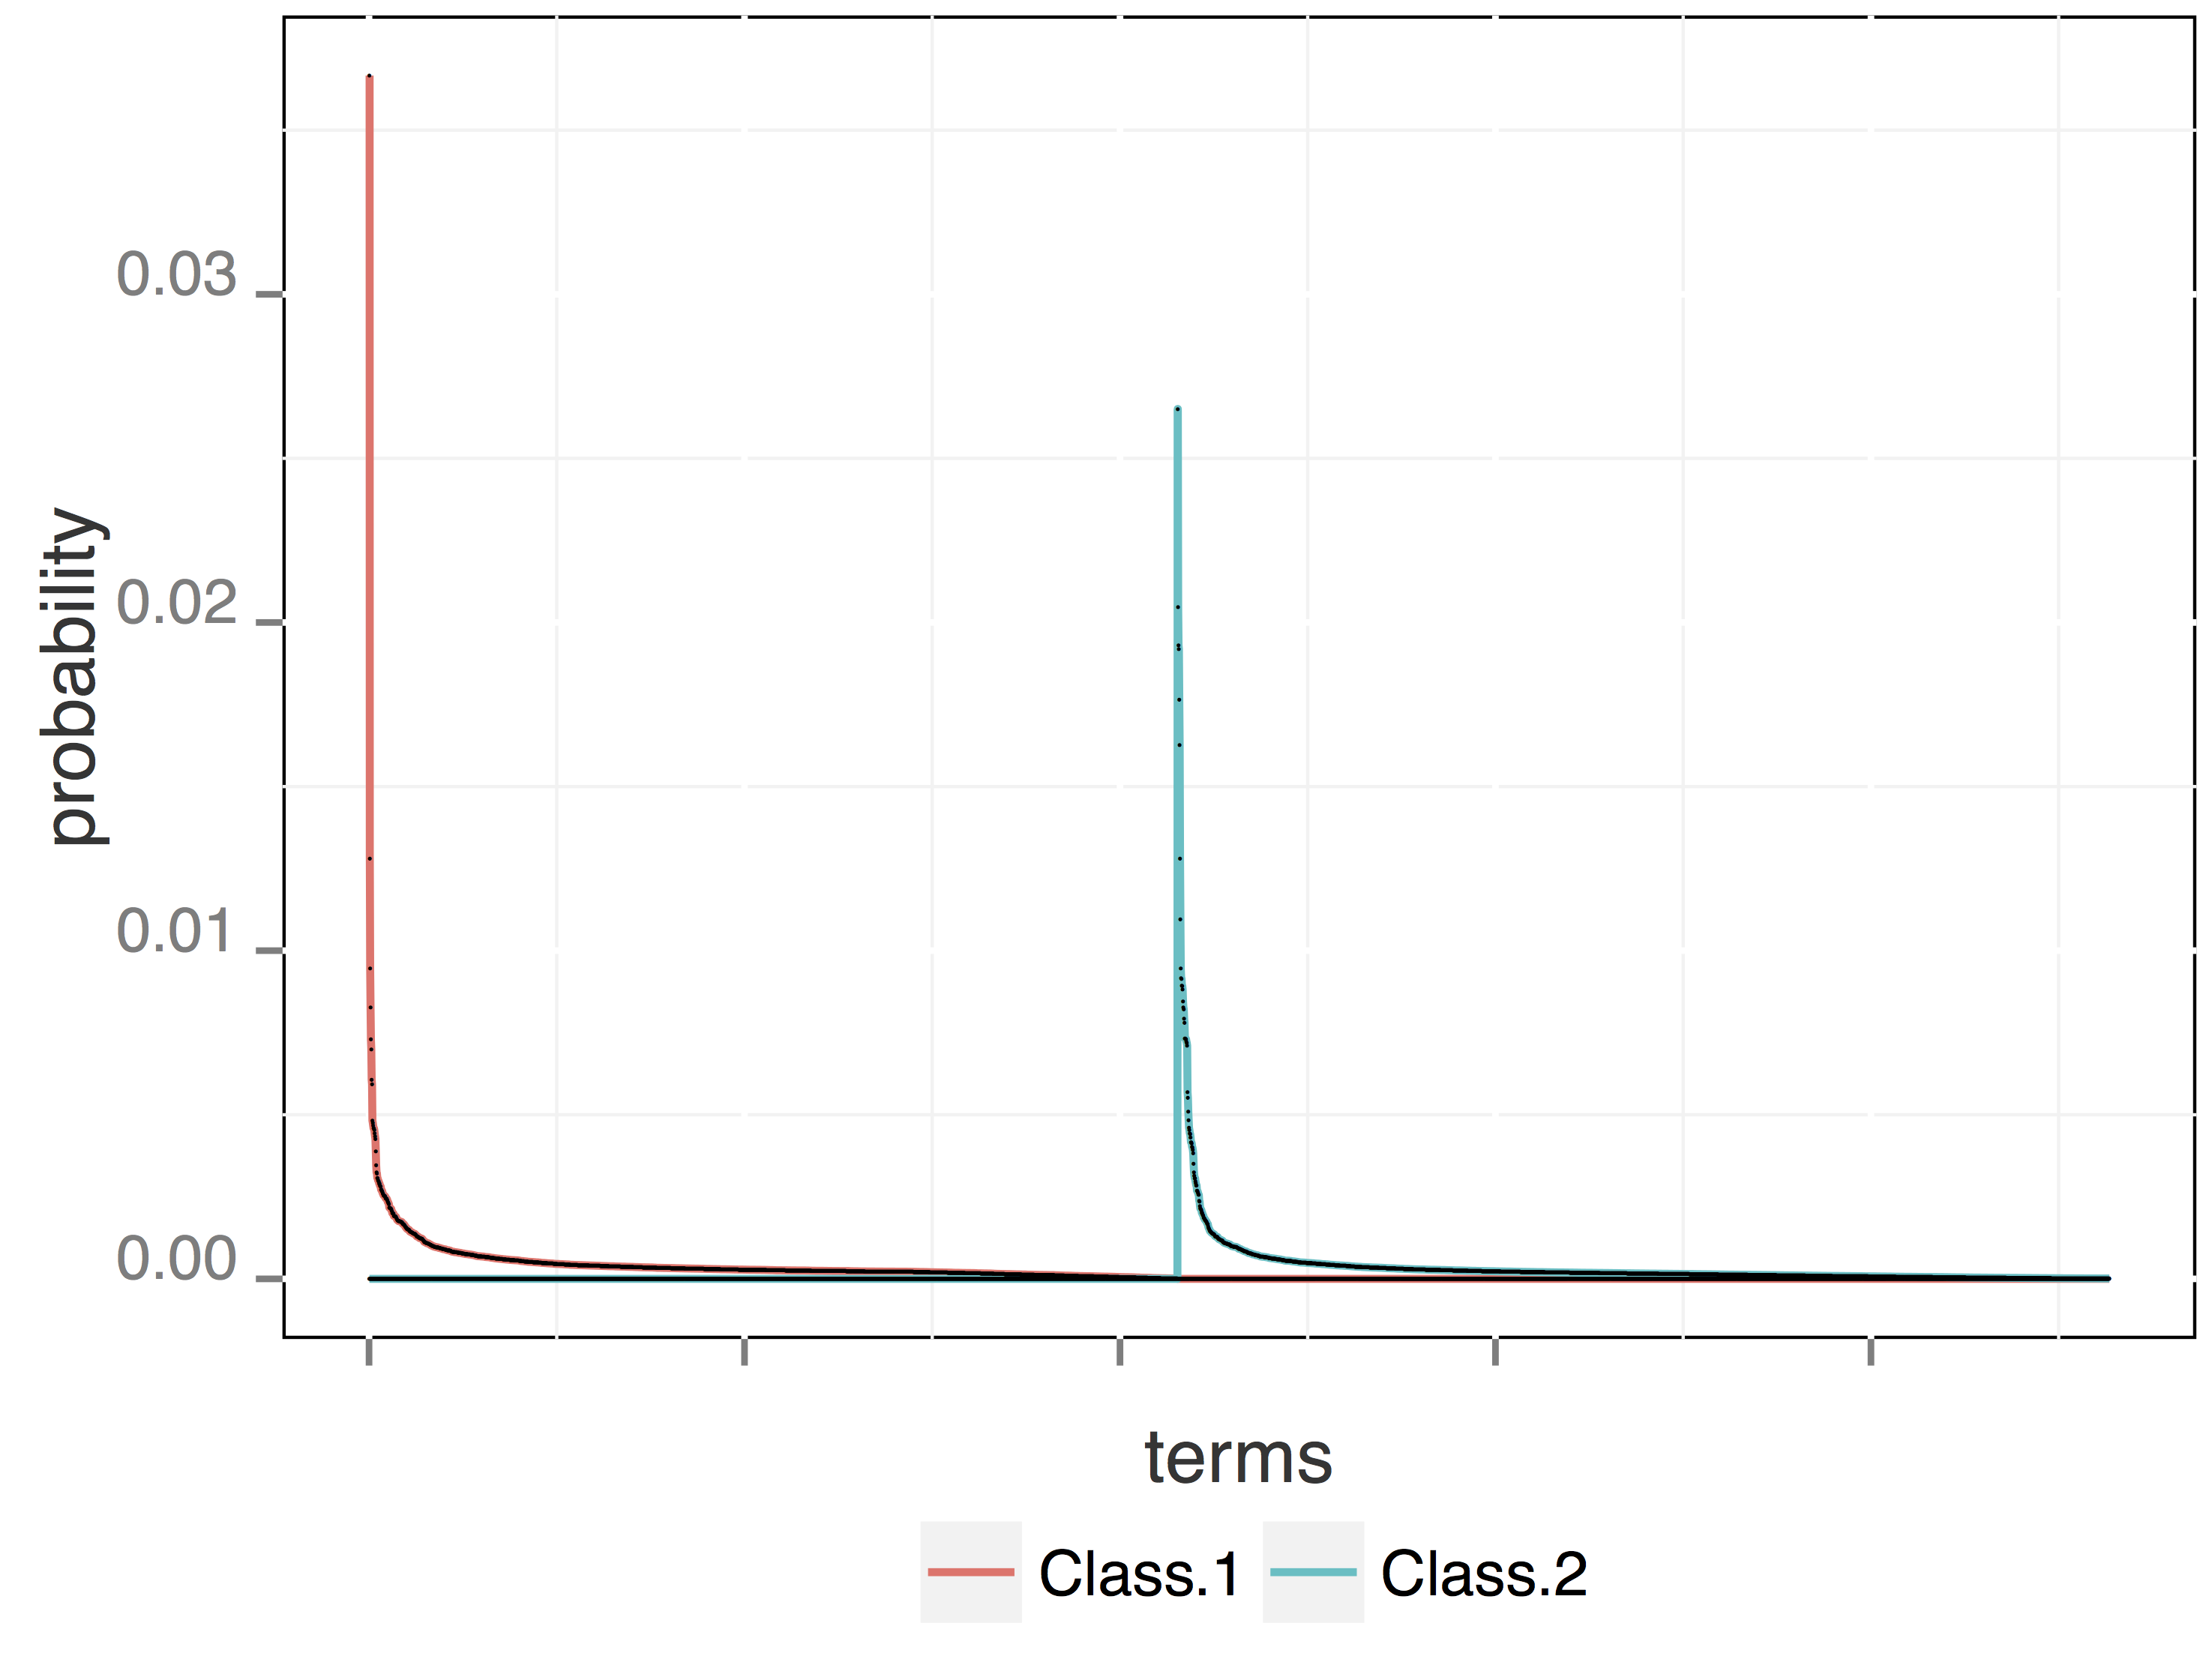
\includegraphics[width=\linewidth]{02-part-01/chapter-03/figs_and_tables/img_example-swlm.png}
\caption{\label{fig:sep-swlm} \scriptsize{A well-separable representation of data}}
\end{subfigure}
\caption{\label{fig:sep_rep} Probability distribution over terms for data in two different classes, (entities in the statues layer of the parliament), sorted based on the term weights in one of the classes.}
% }
\end{figure}
Separation in the data or feature space is a favorable property that not only helps to improve for ranking or classification algorithms but also brings out characteristic features for human inspection.
Figures~\ref{fig:sep-slm} and ~\ref{fig:sep-swlm} illustrate two different ways of modeling two entities in the status layer of the parliamentary hierarchy, i.e., government and opposition. 
Each model is a probability distribution over terms (language model) based on the speeches given by all the members in the corresponding status. In each figure, we sort the terms based on their weights in one of the models and plot the other in the same order. 
%
As can be seen, although distributions over terms in Figure~\ref{fig:sep-slm} for two classes are different, they do not suggest highly separable representations for classes. However, estimated language models in Figure~\ref{fig:sep-swlm} provide highly separable distributions over terms for two classes, identifying the characteristic terms that uniquely represent each class, and can be directly interpreted.  
 
Besides effectiveness and intractability, two\:-\:dimensional separability in the representation of hierarchical entities leads to robust models. This is due to the fact that these representations only capture solid features that remain valid even as the structure of hierarchy changes.
As an example of the importance of robust representations in evolving hierarchies, assume we would learn a representation for the ``US president'' over the current data. This is obvious that we need to distinguish the role in office from the person who is the current president; otherwise the learn representation would not be valid after the next election.  If we can separate the model of the function from the model of the person fulfilling it, for example by abstracting over several presidents, that would in principle be robust over time.

\subsection{Detailed Research Questions}
We break down our main research question in this chapter into three concrete research questions:
\begin{resqbox}
\begin{enumerate}
\item[\textbf{RQ3.1}] \emph{\resq{c3.1}}
\item[\textbf{RQ3.2}] \emph{\resq{c3.2}}
\item[\textbf{RQ3.3}] \emph{\resq{c3.3}}
\end{enumerate}
\end{resqbox}
In the following sections, we will address these research questions.

\section{Separability in the Hierarchies}
\label{sec:sep}
In this section, we explore the first research question in this chapter:
\resq{c3.1}

In addition to the investigation of the separation property as a general foundational property of classification and defining a \emph{\ssp}, we discuss the two\:-\:dimensional separation property of hierarchical classification.

\subsection{Separation Property}
Separability is a highly desirable property for constructing and operating autonomous information systems \citep{Lewis:1995}, and especially classifiers. 
Here, we present a step by step argument which shows that based on the classification principles, having better separability in the feature space leads to better accuracy in the classification results.

%Reasoning steps:
% 0) principles:
Based on the \emph{Probability Ranking Principle (PRP)} presented by \citet{Robertson:1977}, \citet{Lewis:1995} has formulated a variant of PRP for binary classification:

\begin{displayquote}
\emph{For a given set of items presented to a binary classification system, there exists a classification of the items such that the probability of class membership for all items assigned to the class is greater than or equal to the probability of class membership for all items not assigned to the class, and the classification has optimal expected effectiveness.}
\end{displayquote}

Since in many applications, autonomous systems need to decide how to classify an individual item in the absence of entire items set, Lewis has extended the PRP to the \emph{Probability Threshold Principle (PTP)}:

\begin{displayquote}
\emph{For a given effectiveness measure,
there exists a threshold $p$, $0<p<1$, such that for any set of items, if all and only those items with probability of class membership greater than $p$ are assigned to the class, the expected effectiveness of the classification will be the best possible for that set of items.}
\end{displayquote}

PTP, in fact, discusses optimizing the effectiveness of classifiers by making items separable regarding their probability of class membership, which is a discussion on ``separability in the score space''. Based on PTP, optimizing a threshold for separating items is a theoretically trivial task; however, there are practical difficulties. 

% 1) Difficult to achieve the optimum threshold in practice (why?):
The main difficulty refers to the fact that retrieval models are not necessarily capable of measuring actual probabilities of relevance for documents \citep{Arampatzis:2001}, so they do not guarantee to generate a set of scores from which the optimum cutoff can be inferred. 
% 2) Emerging research to deal with this difficulty (analyzing score distributions of rel/irrel):
In this regard, a great deal of work has been done on analyzing the score distribution over relevant and non-relevant documents to utilize this information for finding the appropriate threshold between relevant and non-relevant documents \citep{Kanoulas:2009,Arampatzis:2009,Arampatzis:2001}. 
% 3) separability in scores distributions makes threshold finding easier -> separation property is desirable in score space!
%
It is a clear fact that the more the score distributions of relevant and non-relevant documents are separable, the easier it is to determine the optimum threshold. 
So, obtaining the \emph{separation property} in the scores distributions of relevant and non-relevant documents is one of the key focus areas for retrieval models.

% 4) separability of scores is directly related to the score generating function. But changing score generation functions to generate separable scores are complex -> instead: we can serve score functions with separable terms distribution -> then, since term dist. is a direct sign of relevancy, based on PRP, score functions are supposed to generate separable scores.
There are two ways to obtain separability in the scores distributions.  We could address the complex underlying process of score generation and investigate ranking functions that yield a separable score distribution, as in the score distributional approaches \citep{Arampatzis:2001}.  Alternatively, we can investigate ways to provide existing scoring functions with a highly separable representation of the data. 
That is, the ``term distribution'' directly provides information about the ``probability of relevance'' \citep{Crestani:1998} and if there are separable distributions over $terms$ of relevant and non-relevant documents, a scoring function satisfying PRP will generate scores that separate the classes of relevant and non-relevant documents. 
% 6)So, separation property in feature space is favorable -> Done!
Thus, a \emph{separation property} on feature distribution for representing the data is a favorable property, which follows better accuracy of classifiers' decisions.

In this chapter, we investigate the role of separation in the term or feature spaces, in which we introduce a formal definition for separability and formulate a principle on the effectiveness of classification based on separation property and leave a more formal treatment to future work.
 
As a formal and general definition, we can refer to the model separability as follows:

\begin{mydef}
\label{def:sep}
The model of an entity is epistemologically ``{separable}'' if, and only if, it has %possesses adequate 
unique, non\:-\:overlapping features that distinguish it from other models.
\end{mydef}

We argued that how separability in feature space leads to the separability in score space. Based on this and the given definition of the separability, we present \emph{\ssp (\acssp)}, which is a counterpart of the PTP~\citep{Lewis:1995} in the feature space:

\begin{displayquote}
\emph{For a given set of items presented to a classification system, for each class there exists at least one feature $\delta$ in the representation of items, and a threshold $\tau$, such that for any set of items, if all and only those items with $\delta > \tau$ are assigned to the class, the classification will have the optimal possible performance for that set of items in terms of a given effectiveness measure.}
\end{displayquote}

\acssp, in general, is a stronger version of PTP. In strict binary classification, if you have PTP, which holds on the whole feature space, \acssp will be satisfied, however in the multi-class case, \acssp is stronger and it implies PTP, but not the other way around.
Based on PTP, there is always an underlying probabilistic scoring function on the set of \emph{whole} features, which generates membership probabilities as the scores of items and these scores make items separable with regards to a threshold. So, the scoring function can be deemed as a mapping function which maps items to a new feature space in which the score of each item is a single feature representation of that item (membership probabilities (or scores) in PTP would be equivalent to $\delta$ in \acssp). Thus, when the \acssp holds, the PTP and PRP will also hold.  One could envision a stronger version of the \acssp in which ``all'' the features in the representations need to be non-overlapping, but the \acssp is sufficient for optimizing the effectiveness of the classifier.  The separation principle can be formally extended to hierarchical classification in a straightforward way.  In the rest of this section, we will discuss the separation property in the hierarchical classification and explain how to estimate separable representations with the aim of satisfying \acssp in order to improve the classification effectiveness.

\subsection{Horizontal and Vertical Separability}
\label{subsec:vhs}

In hierarchical text classification, there are two types of boundaries existing in the data, horizontal boundaries, and vertical boundaries. Hence, a separation property should be established in two dimensions. It means, not only separation between entities' representation in one layer is required, but also the separation between the distribution of terms in different layers is needed.

The separation between entities in the same layer is a related concept to the fundamental goal of all classifiers on the data with a flat structure, which is making the data in different classes distinguishable~\citep{Sebastiani:2002}. However, separation between entities in different layers is a concept related to difference of abstraction level and modeling data in different layers in a separable way can help the scoring procedures to figure out the meaning behind the layers and make their decisions less affected by the concepts of other unrelated layers, thus leading to conceptually cleaner and theoretically more accurate models.

Based on Definition~\ref{def:sep}, we formally define horizontal and vertical separability in the hierarchy as follows:
\begin{mydef}
The model of an entity in the hierarchy is ``horizontally separable'' if, and only if, it is \emph{separable} compared to other entities in the same layer, with the same abstraction level.
\end{mydef}

\begin{mydef}
The model of an entity in the hierarchy is ``vertically separable'' if, and only if, it is \emph{separable} compared to other entities in the other layers, with different abstraction levels.
\end{mydef}

To formalize these concepts, consider we have a simple three layers hierarchy of text documents with ``IsA'' relations, where the individual documents take place in the lowest layer, and each node in the middle layer determines a category, representing a group of documents, i.e., its children, and the supernode on the top of the hierarchy deemed to represent all the documents in all the groups in the hierarchy. 
%
There is a key point in this hierarchy to which we will refer for estimating models for the hierarchical entities: ``each node in the hierarchy is a general representation of its descendants''.

First assume that the goal is to estimate a language model representing category $c$, as one of the entities in the middle layer of the hierarchy, and we need the estimated model possessing \emph{horizontal separability}. 
To estimate a horizontally separable model of a category, which represents the category in a way that it is distinguishable from other categories in the middle layer, the key strategy is to eliminate terms that are common across all the categories (overlapping features) and preserve only the discriminating ones.

To do so, we consider there is a general model that captures all the \emph{common} terms of all the categories in the middle layer, $\theta_c^{g}$.  Also we assume that the standard language model of $c$, i.e the model estimated  from concatenation of all the documents in $c$ using MLE, $\theta_{c}$, is drawn from the mixture of the \emph{latent horizontally separable model}, $\theta_{c}^{hs}$, and general model that represents shared terms of all categories, i.e. $\theta_c^{g}$:
\begin{equation}
p(t|\theta_{c})  =  \lambda p(t|\theta_{c}^{hs}) + (1-\lambda) p(t|\theta_c^g),
\end{equation}
%
where $\lambda$ is the mixture coefficient.
Regarding the meaning of the relations between nodes in the hierarchy, top node in the hierarchy is supposed to be a general representation of all categories. On the other hand $\theta_c^{g}$ supposed to be a model capturing general features of all the categories in the middle layer. Thus, we can approximate $\theta_c^{g}$ with the estimated model of the top node in the hierarchy, $\theta_{all}$:
\begin{equation}
 p(t|\theta_c) \approx \lambda p(t|\theta_{c}^{hs}) + (1-\lambda) p(t|\theta_{all}).
 \label{mixture}
\end{equation}

We estimate $\theta_{all}$ using MLE as follows:
\begin{equation}
p(t|\theta_{all}) = \frac{tf(t,all)}{\sum_{t'} tf(t',all)} = \frac{\sum_{c \in all}{\sum_{d \in c}{tf(t,d)}}}{{\sum_{c \in all}{\sum_{d \in c}{\sum_{t' \in d}{tf(t',d)}}}}},
\label{eq:cmodel}
\end{equation}
where $tf(t,d)$ indicates the frequency of term $t$ in document $d$ and $\theta_{all}$ is in fact collection language model. 

Now, the goal is to extract $\theta_{c}^{hs}$. With regard to the generative models, when a term $t$ is generated using the mixture model in Equation~\ref{mixture}, first a model is chosen based on $\lambda$ and then the term is sampled using the chosen model.  The log-likelihood function for generating the whole category $c$ is:
\begin{equation}
\log p(t|\theta_{c}^{hs}) = \sum_{t \in c} tf(t,c) \log \big(\lambda p(t|\theta_{c}^{hs}) + (1-\lambda) p(t|\theta_{all})\big),
\end{equation}
where $tf(t,c)$ is the frequency of occurrence of term $t$ in category $c$. 
%Setting the parameter $\alpha$ to a fixed value and 
With the goal of maximizing this likelihood function, the maximum likelihood estimation of $p(c|\theta_{c}^{hs})$ can be computed using the Expectation-Maximization (EM) algorithm by iterating over the following steps:
\\
\textbf{E-step:}
\begin{equation}
e_t = tf(t|c).\frac{\lambda p(t|\theta_{c}^{hs})}{\lambda p(x|\theta_{c}^{hs}) + (1-\lambda) p(x|\theta_{all})}
\label{EM-E},
\end{equation}
\textbf{M-step:}
\begin{equation}
p(x|\theta_{c}^{hs}) = \frac{e_t}{\sum_{t' \in \mathcal{V}} e_t'}, \mathrm{~i.e.~normalizing~the~model},
\label{EM-M}
\end{equation}
where $\mathcal{V}$ is the set of all terms with non-zero probability in $\theta_c$. In Equation~\ref{EM-E}, $\theta_c$ is the maximum likelihood estimation of category $c$: $p(t|\theta_{c}) = \nicefrac{\sum_{d \in c}c(t,d)}{\sum_{d \in c}{\sum_{t' \in d} c(t',d)}}$ and $\theta_{c}^{hs}$ represents the horizontally separable model, which in the first iteration it is initialized by the maximum likelihood estimation, similar to $\theta_c$. 

Considering the above process, a horizontally separable model is a model which is \textbf{specified} by taking out general features that have a high probability in ``all'' categories or let's say collection language model, which is similar to the concept of the parsimonious language model, introduced by~\citet{Hiemstra:2004}.

Now assume that we want to extract a language model possessing \emph{vertical separability} for the category $c$, i.e., a model that makes this category distinguishable from entities both in the lower layer (each individual document) and the top layer (collection of all documents).
%
In the procedure of making the model horizontally separable, we argued that we can reduce the problem to removing terms representing the top node, which results in a model that is separable from the top node in the upper layer. This means that we are already half-way towards making a model vertically separable; thus, the model only requires to be separable from its descendant entities in the lower layer.  
Back to the meaning of the ``IsA'' relations in the hierarchy, the model of each node is a general representation of all its descendants. So making the model of a category separable from its descendant documents means to remove terms that describe each individual documents, but not all of them. We call these terms, document specific terms.

For each category $c$, we assume there is a  model, $\theta_d^{s}$, that captures document specific terms, i.e. terms from documents in that category that are good indicators for individual documents but not supported by all of them. Also we assume that the standard language model of $c$, $\theta_{c}$, is drawn from the mixture of the \emph{latent vertically separable model}, $\theta_{c}^{vs}$, and $\theta_d^{s}$: 
\begin{eqnarray}
p(t|\theta_{c}) & = & \lambda p(t|\theta_{c}^{vs}) + (1-\lambda) p(t|\theta_d^s)
\end{eqnarray}
where $\lambda$ is the mixing coefficient. 
We estimate $\theta_d^s$ using the following equation:
\begin{equation}
p(t|\theta_d^s)  \xleftarrow{normalized} 
\sum_{d_i\in c} 
\bigg(
p(t|\theta_{d_i}) \prod_{\substack{d_j\in c \\ j \neq i}} (1-p(t|\theta_{d_j}))
\bigg),
\label{eq:smodel}
\end{equation}
where $p(t|\theta_{d_i}) = \nicefrac{c(t,d_i)}{\sum_{t' \in d_i} c(t',d_i)}$. This equation assigns a high probability to a term if it has high probability in one of the document models, but not others, marginalizing over all the document models.  This way, the higher the probability is, the more specific the term will be. 
Now, the goal is to extract the $\theta_{c}^{vs}$. An EM algorithm, similar to Equations~\ref{EM-E} and~\ref{EM-M} can be applied for estimating $\theta_{c}^{vs}$ by removing the effect of $\theta_d^s$ from $\theta_{c}$.

Considering the above process, a vertically separable model is a model which is \textbf{generalized} by taking out specific terms that have a high probability in one of the descendant documents, but not others.  

\subsection{Two\:-\:Dimensional Separability}
In order to have fully separable models in hierarchical classification, they should own two\:-\:dimensional separation property. We define two\:-\:dimensional separability as follows:
\begin{mydef}
The model of an entity in the hierarchy is ``two\:-\:dimensionally separable'' if, and only if, it is both horizontally and vertically separable at the same time.
\end{mydef}

Intuitively, if a model of an entity is two\:-\:dimensionally separable, it should capture \emph{all}, and \emph{only}, the essential features of the entity taking its relative position in the hierarchy into consideration.  In the next section, we will discuss how to estimate two\:-\:dimensional separable models for entities in the hierarchies with more than three layers.


\section{\HSWLMs}
\label{sec:hswlm}
In this section, we address the second research question of this chapter:
\resq{c3.2}

We introduce \Hswlms (\achswlm) which is an extension of \SWLM that is explained in chapter~\ref{chap:2} tailored to textual hierarchical entities. \achswlm is, in fact, a particular arrangement of multiple passes of the procedures of making the models of hierarchical entities vertically and horizontally separable, as they are explained in Section~\ref{subsec:vhs}.
%
We use the idea of parsimonious language models \cite{Hiemstra:2004} to parsimonize the representation of an entity by down-weighting terms that do not reflect the significant features of that entity, with regards to its position in the hierarchy.   
In the parsimonious language model, given a raw probabilistic estimation, the goal is to re-estimate the distribution so that non-essential parameters of the raw estimation are down-weighted if they are well explained in a given background distribution. 
The proposed approach for estimating \hswlm iteratively reestimates the standard language models of entities to minimize their overlap by discarding non\:-\:essential terms from them. 

In the original parsimonious language model~\citep{Hiemstra:2004}, the background model is explained by the estimation of the \emph{collection model}, i.e., the model representing all the entities, similar to Equation~\ref{eq:cmodel}.  
However, with respect to the hierarchical structure, and our goal in \achswlm for making the models of entities separable from each other, we need to use the parsimonization technique in two different directions: 1) given ancestors of an entity, and 2) given its descendants. Hence, besides parsimonizing given a single parent entity in the upper layers, as the background model, we need to be able to do parsimonization given multiple descendants in the lower layers. 
\input{02-part-01/chapter-03/figs_and_tables/alg_hswlm_model_parsimonization.tex}
Algorithm~\ref{alg:model_parsimonization} presents pseudo-code of the Expectation-Maximization algorithm which is employed in the modified model parsimonization procedure. 
In the equation in line 3 of the pseudo-code in Algorithm~\ref{alg:model_parsimonization}, $B$ is the set of background entities\:---\:either one or multiple, and $\theta_{b_i}$ demonstrates the model of each background entity, $b_i$, which is estimated using MLE. As can be seen, in case of having a single ancestor node as the background model,  this equation will be equal to Equation~\ref{eq:cmodel} and in case of having multiple descendants as the background models, it results same as Equation~\ref{eq:smodel}. 
In this procedure, in general, in the E-step, the probabilities of terms are adjusted repeatedly, and in the M-step, adjusted probability of terms are normalized to form a distribution. 
Another change in the modified version of model parsimonization, which practically makes no difference in the final estimation, is that in the E-step, instead of using $tf(t,e)$, we employ $p(t|\theta_e)$, where $\theta_e$ is the model represents entity $e$ and initially it is estimated using MLE. This is because in the multi-layer hierarchies, there is more than one parsimonization pass for a particular entity and after the first round, we need to use the probability of terms estimated from the previous pass, not the raw information of their frequency.

\input{02-part-01/chapter-03/figs_and_tables/alg_hswlm.tex}
Model parsimonization is an almost parameter free process. The only parameter is the standard smoothing parameter $\lambda$, which controls the level of parsimonization, so that the lower values of $\lambda$ result in more parsimonious models.
The iteration is repeated a fixed number of times or until the estimates do not change significantly anymore. 

The pseudo-code of the overall procedure of estimating \achswlm is presented in Algorithm~\ref{alg:hswlm}. 
Before the first round of the procedure, a standard estimation like maximum likelihood estimation is used to construct the initial model for each entity in the hierarchy. 
Then, models will be updated in an iterative process until all the estimated models of entities become stable. 
In each iteration, there are two main stages: a \emph{Specification stage} and a \emph{Generalization stage}. 
In these stages, language models of entities in the hierarchy are iteratively made ``specific,'' by taking out terms explained at higher levels, and ``general,'' by eliminating specific terms of lower layers, which results in models that are both \emph{horizontally} and \emph{vertically} separable as it is described in Section~\ref{subsec:vhs}.

\input{02-part-01/chapter-03/figs_and_tables/alg_hswlm_specification_step.tex}
In the specification stage, the goal is to eliminate the general terms of the language model of each entity so that the resulted language model demonstrates the entity's specific properties.  
To do so, the parsimonization method is used to parsimonize the language model of an entity given its ancestors, from the root of the hierarchy to its direct parent, as the background estimations. 
%
The order in the hierarchy is of crucial importance here. 
When a language model of an ancestor is considered as the background language model, it should demonstrate the ``specific'' properties of that ancestor. Due to this fact, it is important that before considering the language model of an entity as the background estimation, it has already passed the specification stage, and we have to move top-down.
Pseudo\:-\:code of the recursive procedure of specification of entities' models in the hierarchy is depicted in Algorithm~\ref{alg:specification_stage}.

\input{02-part-01/chapter-03/figs_and_tables/alg_hswlm_generalization_step.tex}
In the generalization stage, the goal is to refine language models by removing terms which do not address the concepts in the level of abstraction of the entity's layer.
To do so, again parsimonization is exploited but given descendants, which leads to the elimination of specific terms. 
Here also, before considering the model of an entity as the background estimation, it should be already passed the generalization stage, so generalization moves bottom up.
Algorithm~\ref{alg:generalization_stage} presents the pseudo\:-\:code for the recursive procedure of generalization of entities' language models in the hierarchy. 
In the generalization step, the background models of descendants are supposed to be specific enough to show their extremely specific properties. Hence, generalization stages must be applied on the output models of specification stages: specification should precede generalization, as shown in Algorithm~\ref{alg:hswlm} before.

\section{\achswlm for Hierarchical Classification}
Two-dimensional separability as the main properties of \achswlm makes the learned representations of the entities in the hierarchy less sensitive to the structural changes for instance when the hierarchy evolves over time. Here in this section, we address our last research question of this chapter:
\resq{c3.3}

Before evaluating the transferability of two-dimensionaly separable representations over time, we intrinsically study the separability of the representations learned by \achswlm. We use parliamentary data as one of the interesting collections with hierarchically structured data that can evolve over time. The structure of the parliamentary hierarchy has been shown in Figure~\ref{fig:ParHierarchy}.  First, we introduce the collection we have used, and then we analyze the quality of \achswlm on providing horizontal and vertical separability over the hierarchy. 

\subsection{Data Collection}
We use the Dutch parliamentary data which forms a hierarchical structure that can evolve over time. The data are collected and annotated as the part of
\emph{Political\-Mashup} project \citep{url:politicalmashup} to make semantically enriched parliamentary proceedings available as open data \citep{marx:2010}.

As a brief background, the Dutch parliament is a bicameral parliament which consists of the Senate and the house of representatives. The house of representatives is the main chamber of parliament, where discussion of proposed legislation and review of the government's actions takes place.  The Dutch parliamentary system is a multi-party system, requiring a coalition of parties to form the government~\citep{deswaan73}.

\input{02-part-01/chapter-03/figs_and_tables/fig_ducth_parl_hierarchy.tex}
We use data from the parliament or the House of Representatives of the Netherlands.  We have chosen three interesting periods of parliament, from March 2006 to April 2014, in which eight main parties have about 95\% of seats in the parliament: People's Party for Freedom and Democracy, Labour Party, Christian Democratic Appeal, Party for Freedom, The Socialist Party, Democrats 66, Green-Left, Christian-Union.   The coalition in the first period is between a left-wing party and a centrist party, in the second period between a right-wing party and centrism party, and in the third, between a right-wing and left-wing party. Figure~\ref{fig:DutchParl} shows the hierarchical structure of the Dutch parliament in these three different periods.

In order to learn representations for parliamentary entities, first of all,  we prepare the data. In the proceedings, there are series of parliamentary speeches by different MPs following the debate structure.  We invert the data matrix so that for each speaker we collect their speeches as a single document that reflects the features of that member. Then, for representing the internal entities in the parliament's hierarchy, we first consider members as the leaf entities and then concatenate all leaf documents below internal entities as a single document which textually represents them: first over parties, and then parties into government and opposition, etc.
%
The whole corpus consists of 14.7 million terms from 240,501 speeches and contains 2.1 million unique terms. 
No stemming and no lemmatization is done on the data and also stop words, and common words are not removed in data preprocessing.  After data preparation, we estimate \acswlm\ for all entities in the hierarchy as it is explained in Section~\ref{sec:hswlm}.

%---------------------------------------
\subsection{Two-Dimensional Separability of \achswlm}
\label{subsec:achswlmep}
%---------------------------------------
Here we investigate the ability of \achswlm on providing language models for hierarchical entities that are two-dimensionally separable. 
Based on the explained procedure of estimating \achswlm, the language models of entities in the hierarchy is repeatedly updated, so that the resulting models are both \emph{horizontally} and \emph{vertically} separable in the hierarchy. To assess this fact, we estimate \achswlm on the parliamentary data and look into the separability between entities in the same layer or in different layers.

Figures~\ref{fig:HSS} and~\ref{fig:HSP} illustrate the probability distribution over terms based on the estimated \achswlm in the status and party layer respectively. We sort the probability distribution on the term weight of the first model and plot the other models in this exact order.
As can be seen in the status layer, Figures~\ref{fig:HSS}, the distributions over terms for government and opposition cover almost separated set of terms. Since in this layer these two entities are supposed to be against each other, a high level of separability can be expected. On the other hand, in the party layer, Figures \ref{fig:HSP}, it is possible that two parties share some ideological issues and consequently share some terms. So, in this layer, a complete separability of terms would not be practically possible for all the parties. Nevertheless, \achswlm provides an acceptable horizontal separability in this layer.


\begin{figure}[t]
    \centering
    \begin{subfigure}[b]{0.32\textwidth}
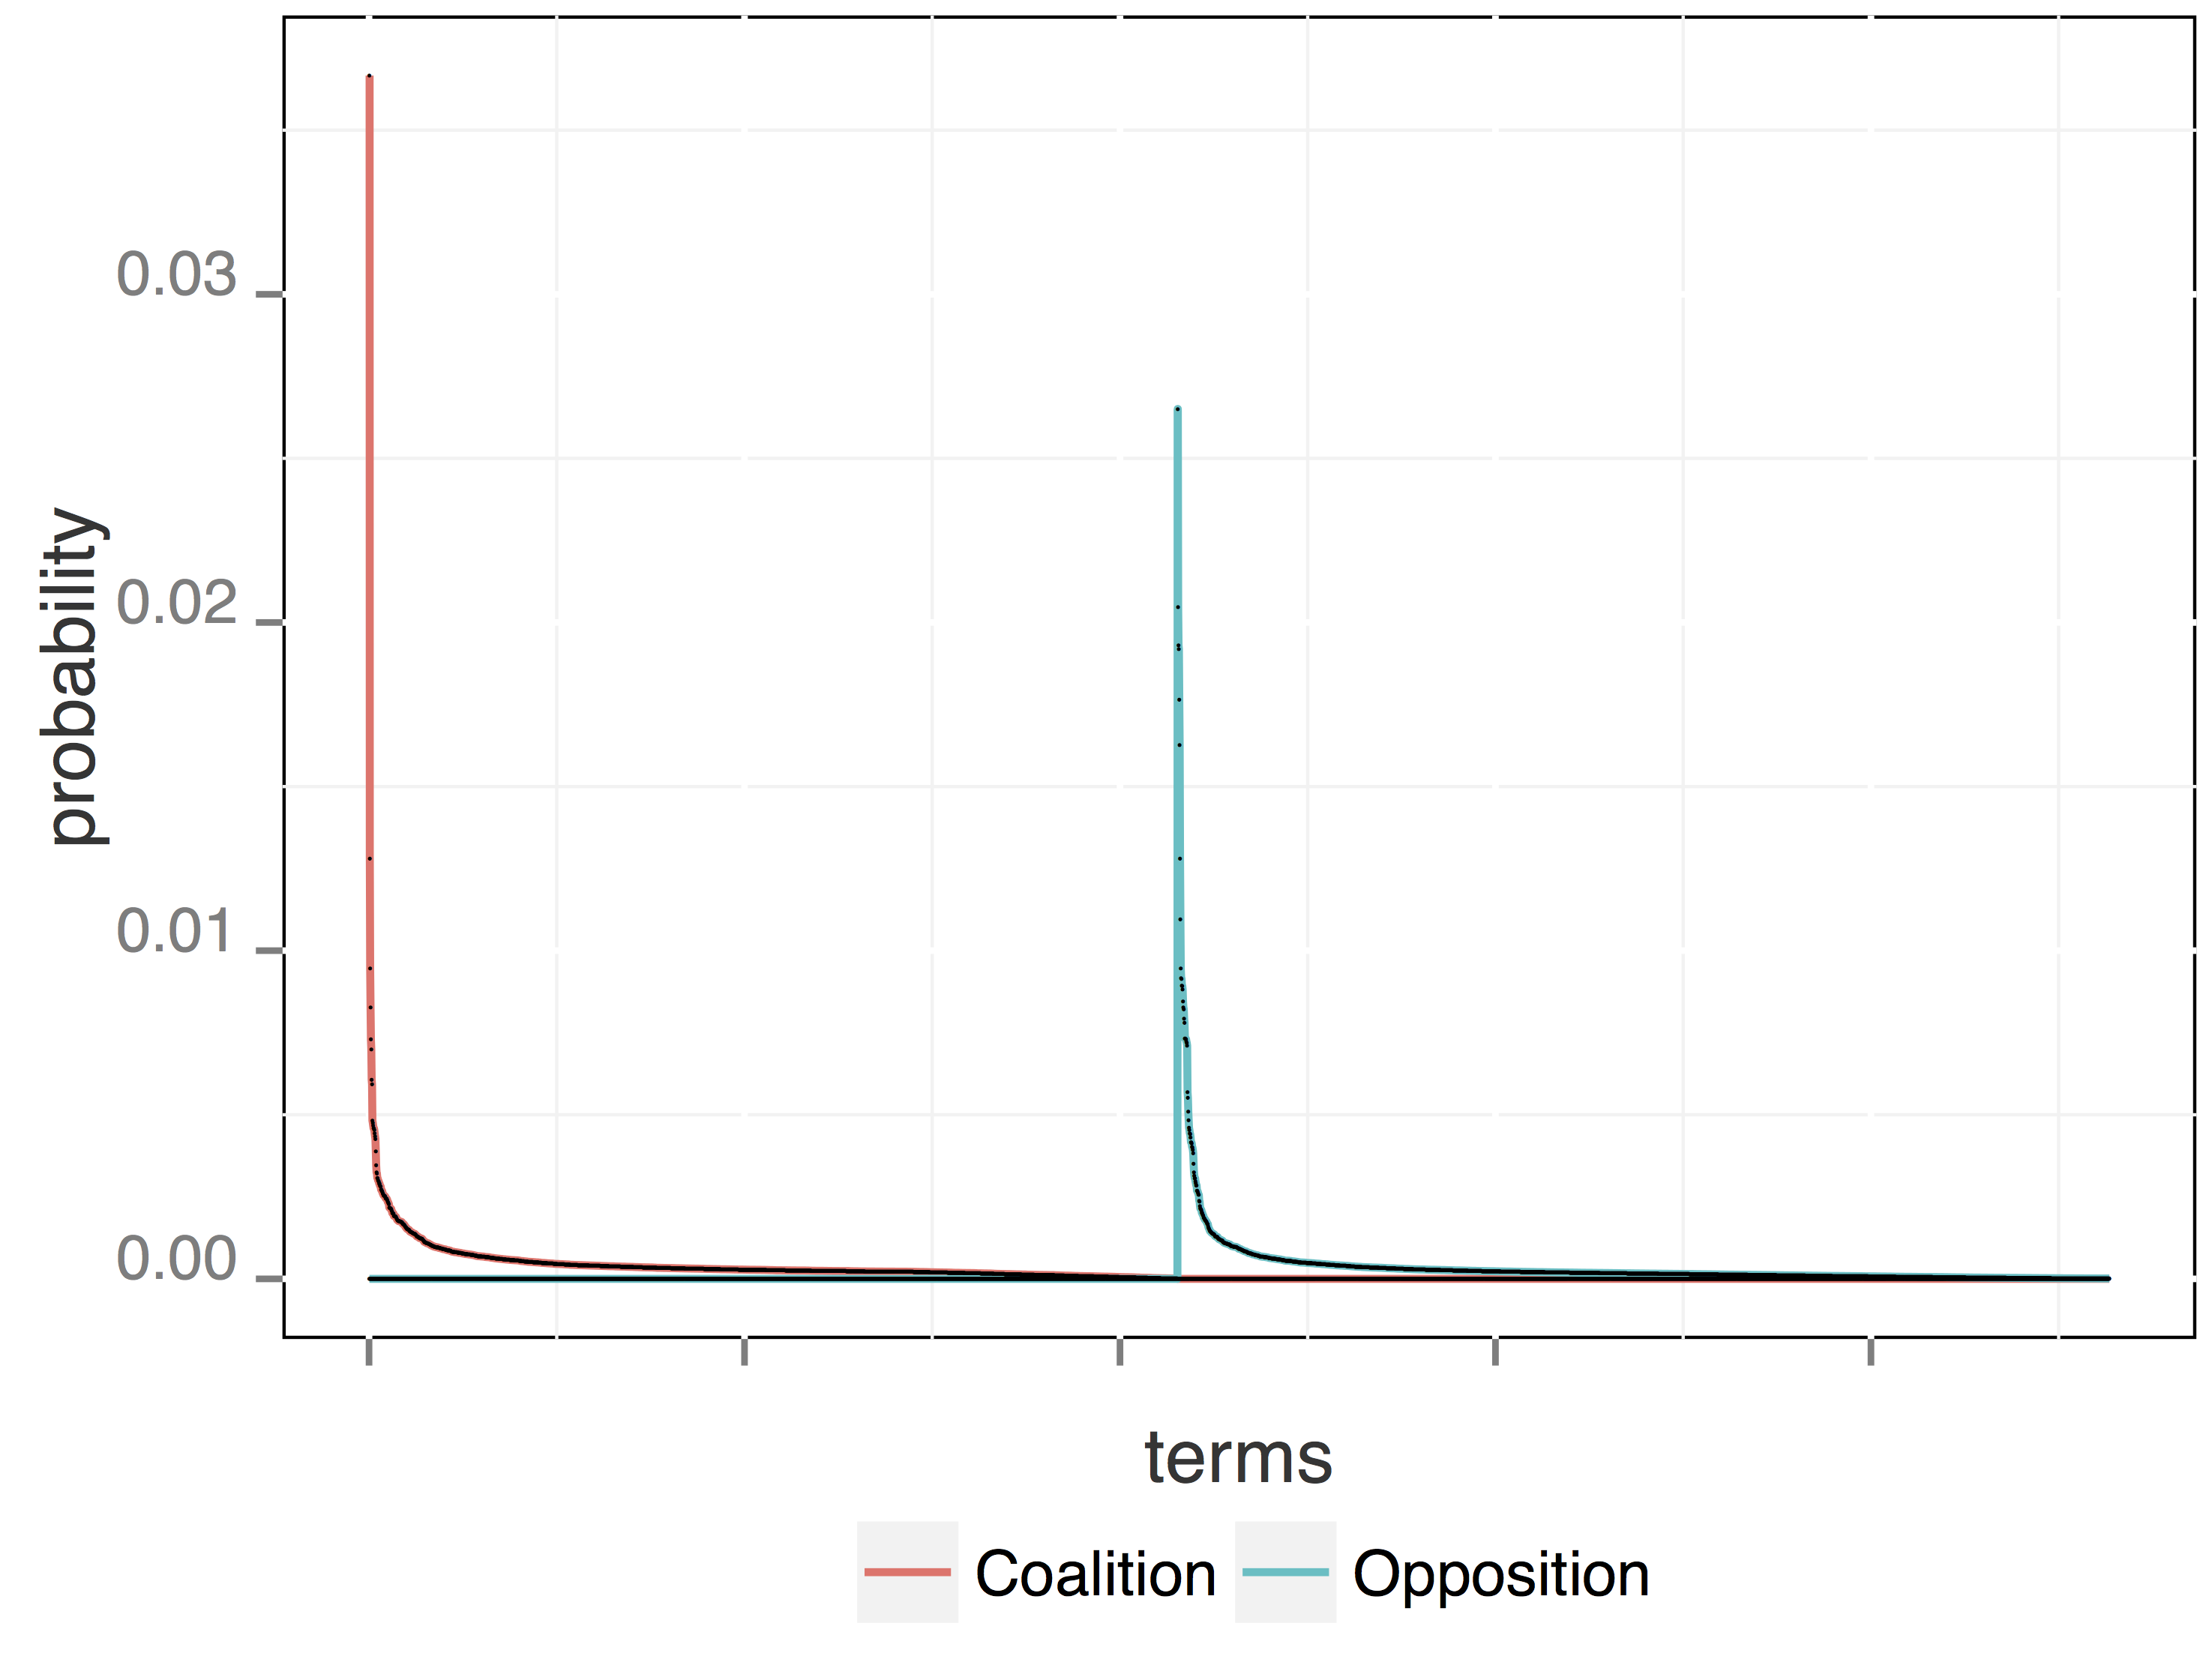
\includegraphics[width=\linewidth]{02-part-01/chapter-03/figs_and_tables/img_opo-coa.png}
\caption{\label{fig:HSS}\achswlm in the status layer}
        \end{subfigure}
        ~ 
    \begin{subfigure}[b]{0.64\textwidth}
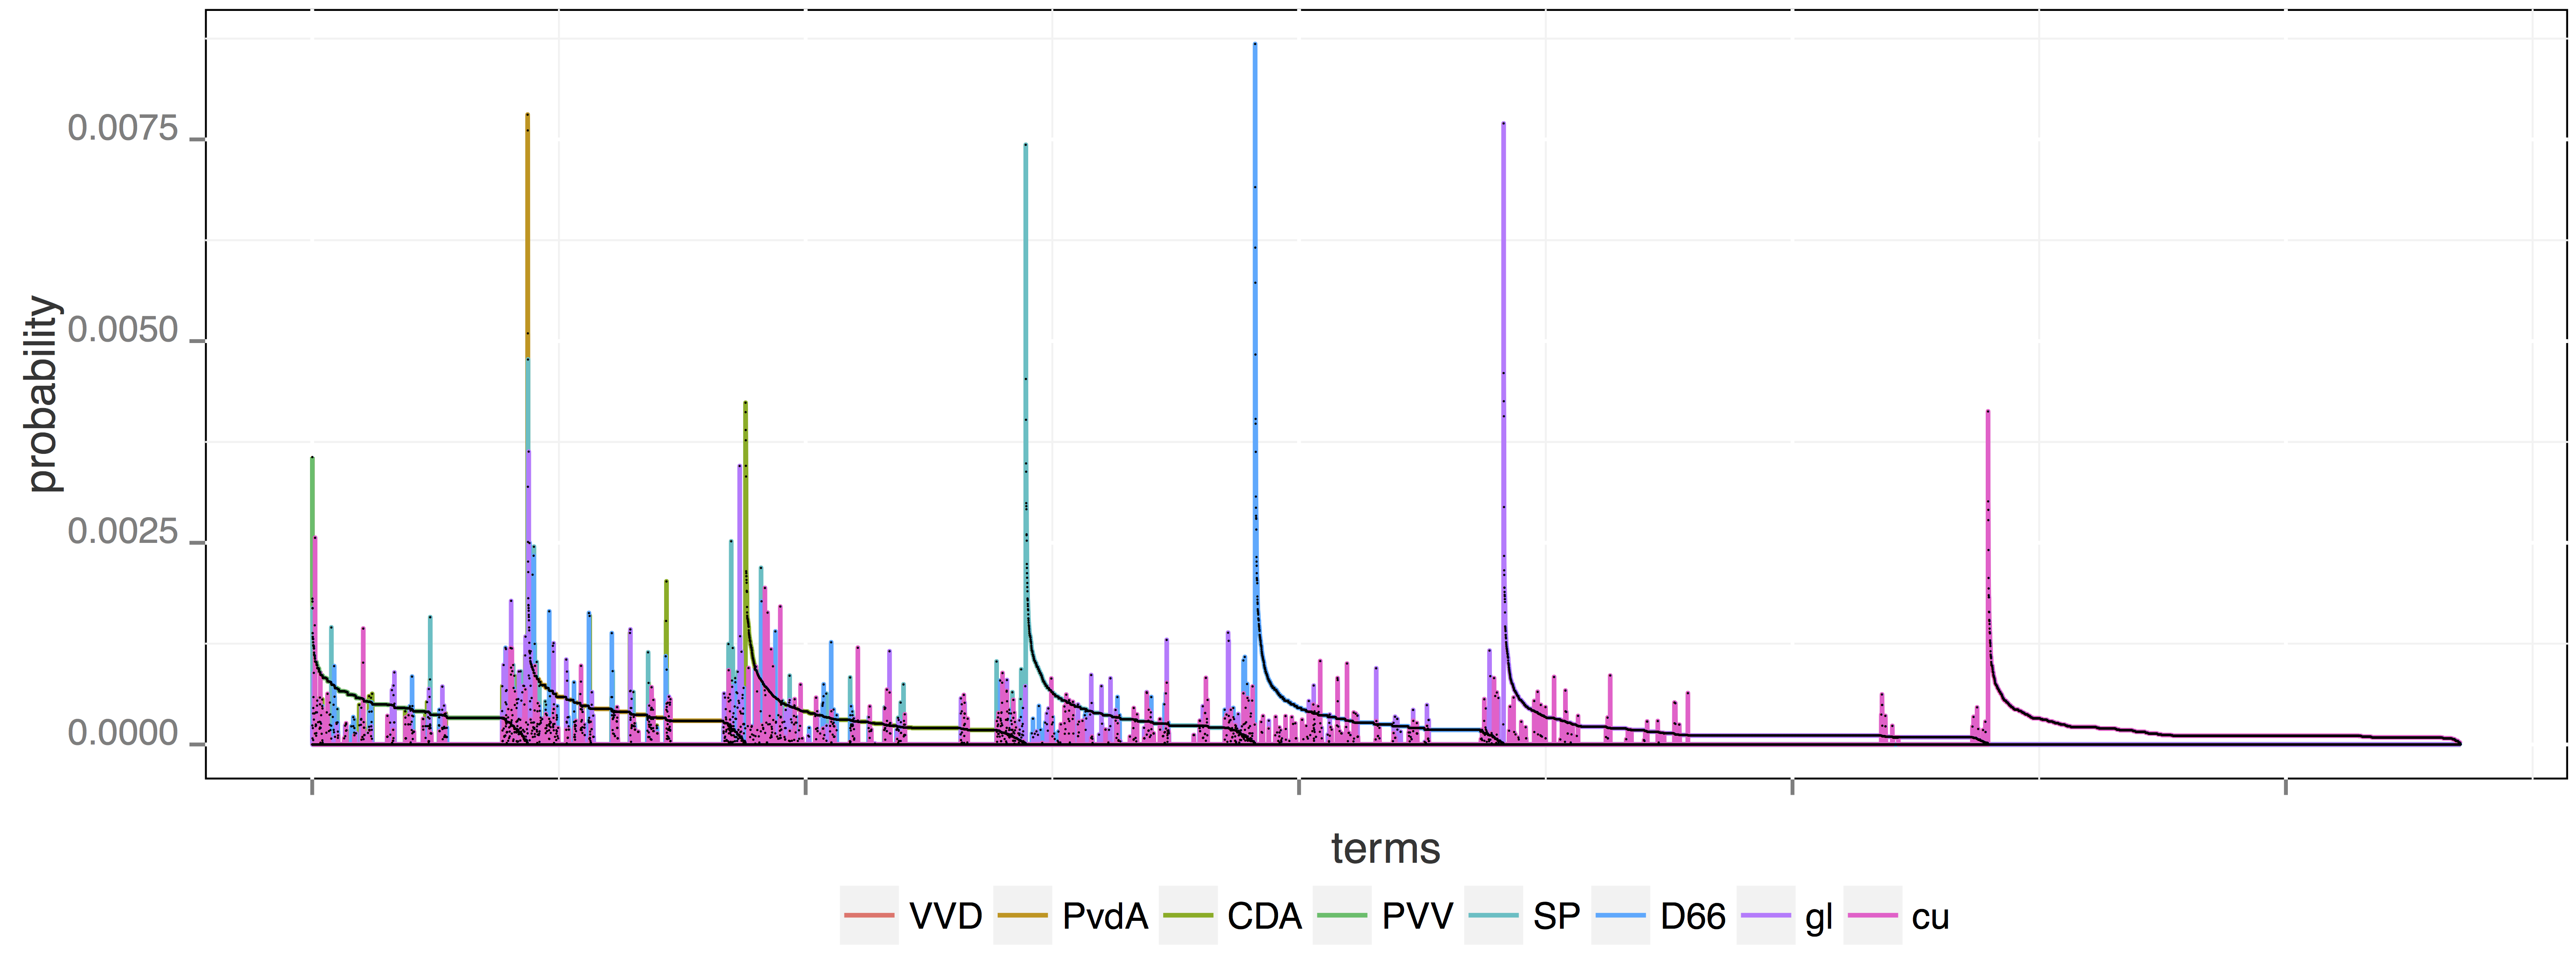
\includegraphics[width=\linewidth]{02-part-01/chapter-03/figs_and_tables/img_parties.png}
\caption{\label{fig:HSP}\achswlm in the party layer}
        \end{subfigure}
    \caption{\label{fig:HS} \emph{Horizontal Separability}: probability distribution over terms based on \hswlms in status layer and party layer.}
\end{figure}

Besides, we illustrate the horizontal separability of \achswlm of some pairs of parties. Figures \ref{fig:HSPCO}, \ref{fig:HSPOO}, and \ref{fig:HSPCC} show the separability of models of two parties in three cases, respectively: 1) different statuses, 2) both in the status of opposition, 3) both in the status of government. It can be seen that in all cases of being in the same status or different status, estimated \hswlms are separable. The interesting point is in Figure~\ref{fig:HSPCC} that presents the models of two government parties that are strongly separable. This rooted in the fact that in this period there was an unusual coalition government consisting of a right-wing and a left-wing party. So, although they have an agreement in the status layer, their model is highly separable in terms of having opposite spectrum in party layer.


\begin{figure}[!t]
        \centering
        \begin{subfigure}[b]{0.32\textwidth}
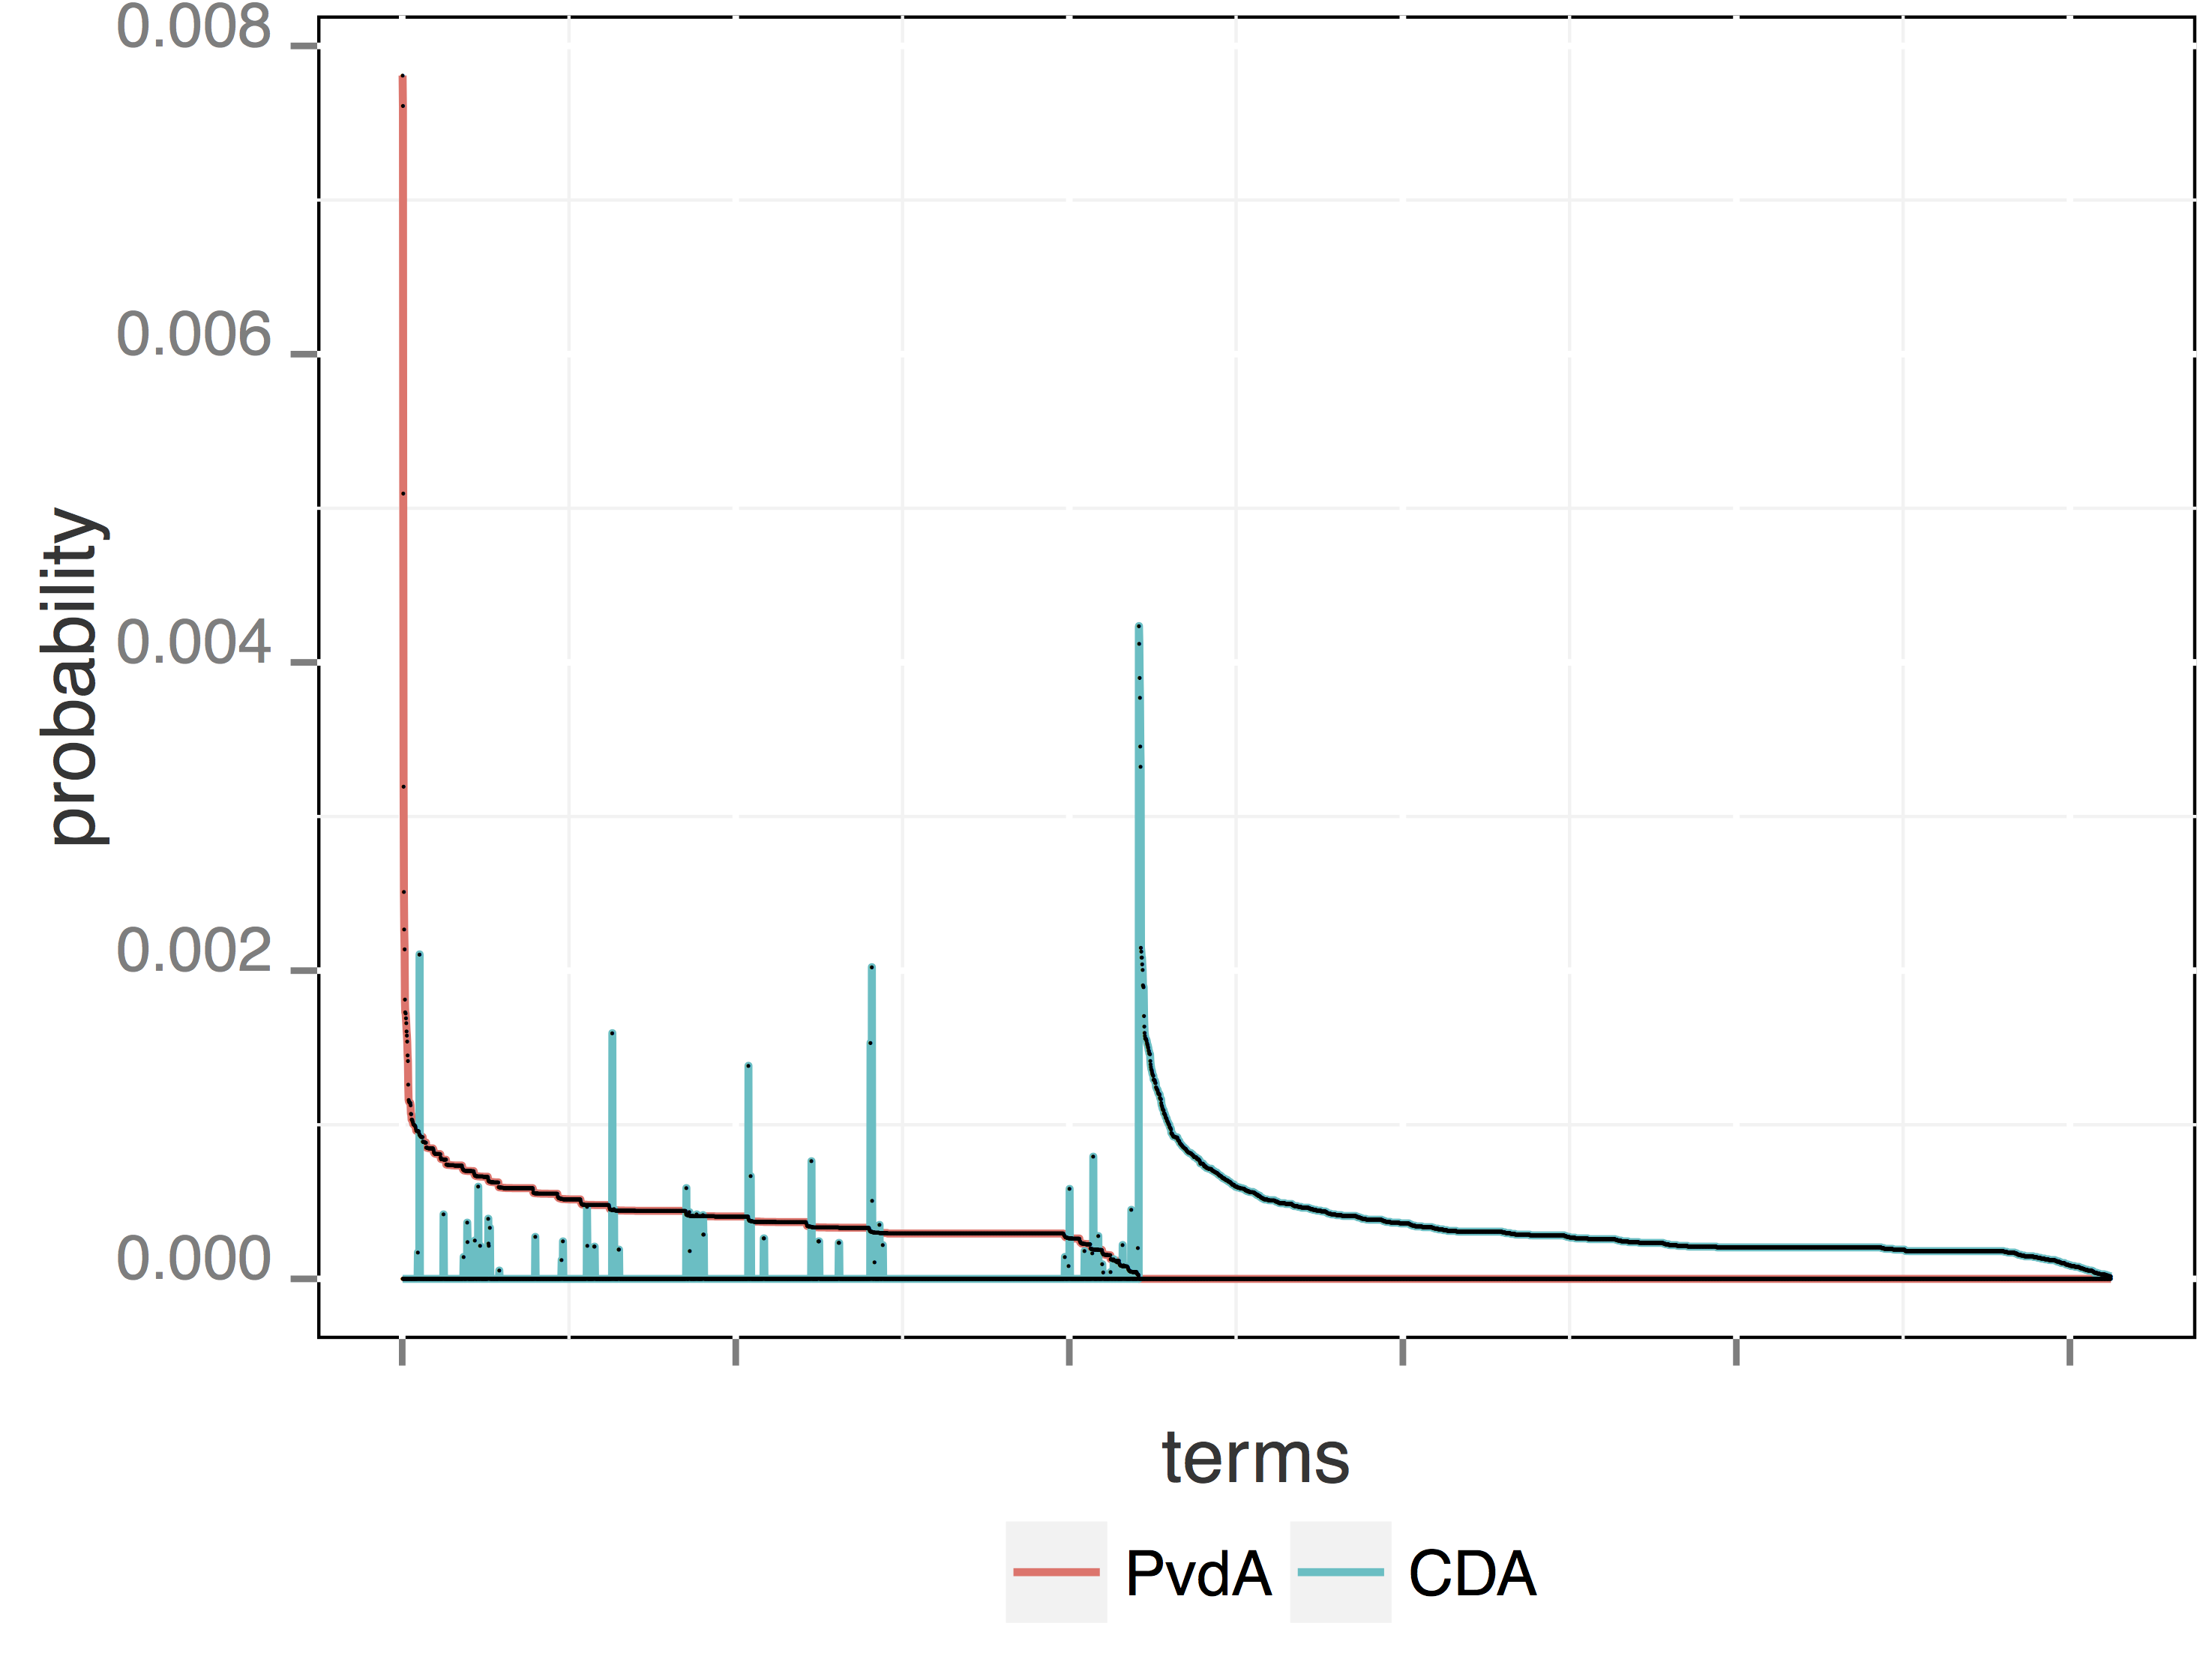
\includegraphics[width=\linewidth]{02-part-01/chapter-03/figs_and_tables/img_PvdA-CDA.png}
\caption{\label{fig:HSPCO} \achswlm of two parties in different statuses: Christian Democratic Appeal (CDA) and Labour Party (PvdA)}
        \end{subfigure}
        ~ 
        \begin{subfigure}[b]{0.32\textwidth}
\centering
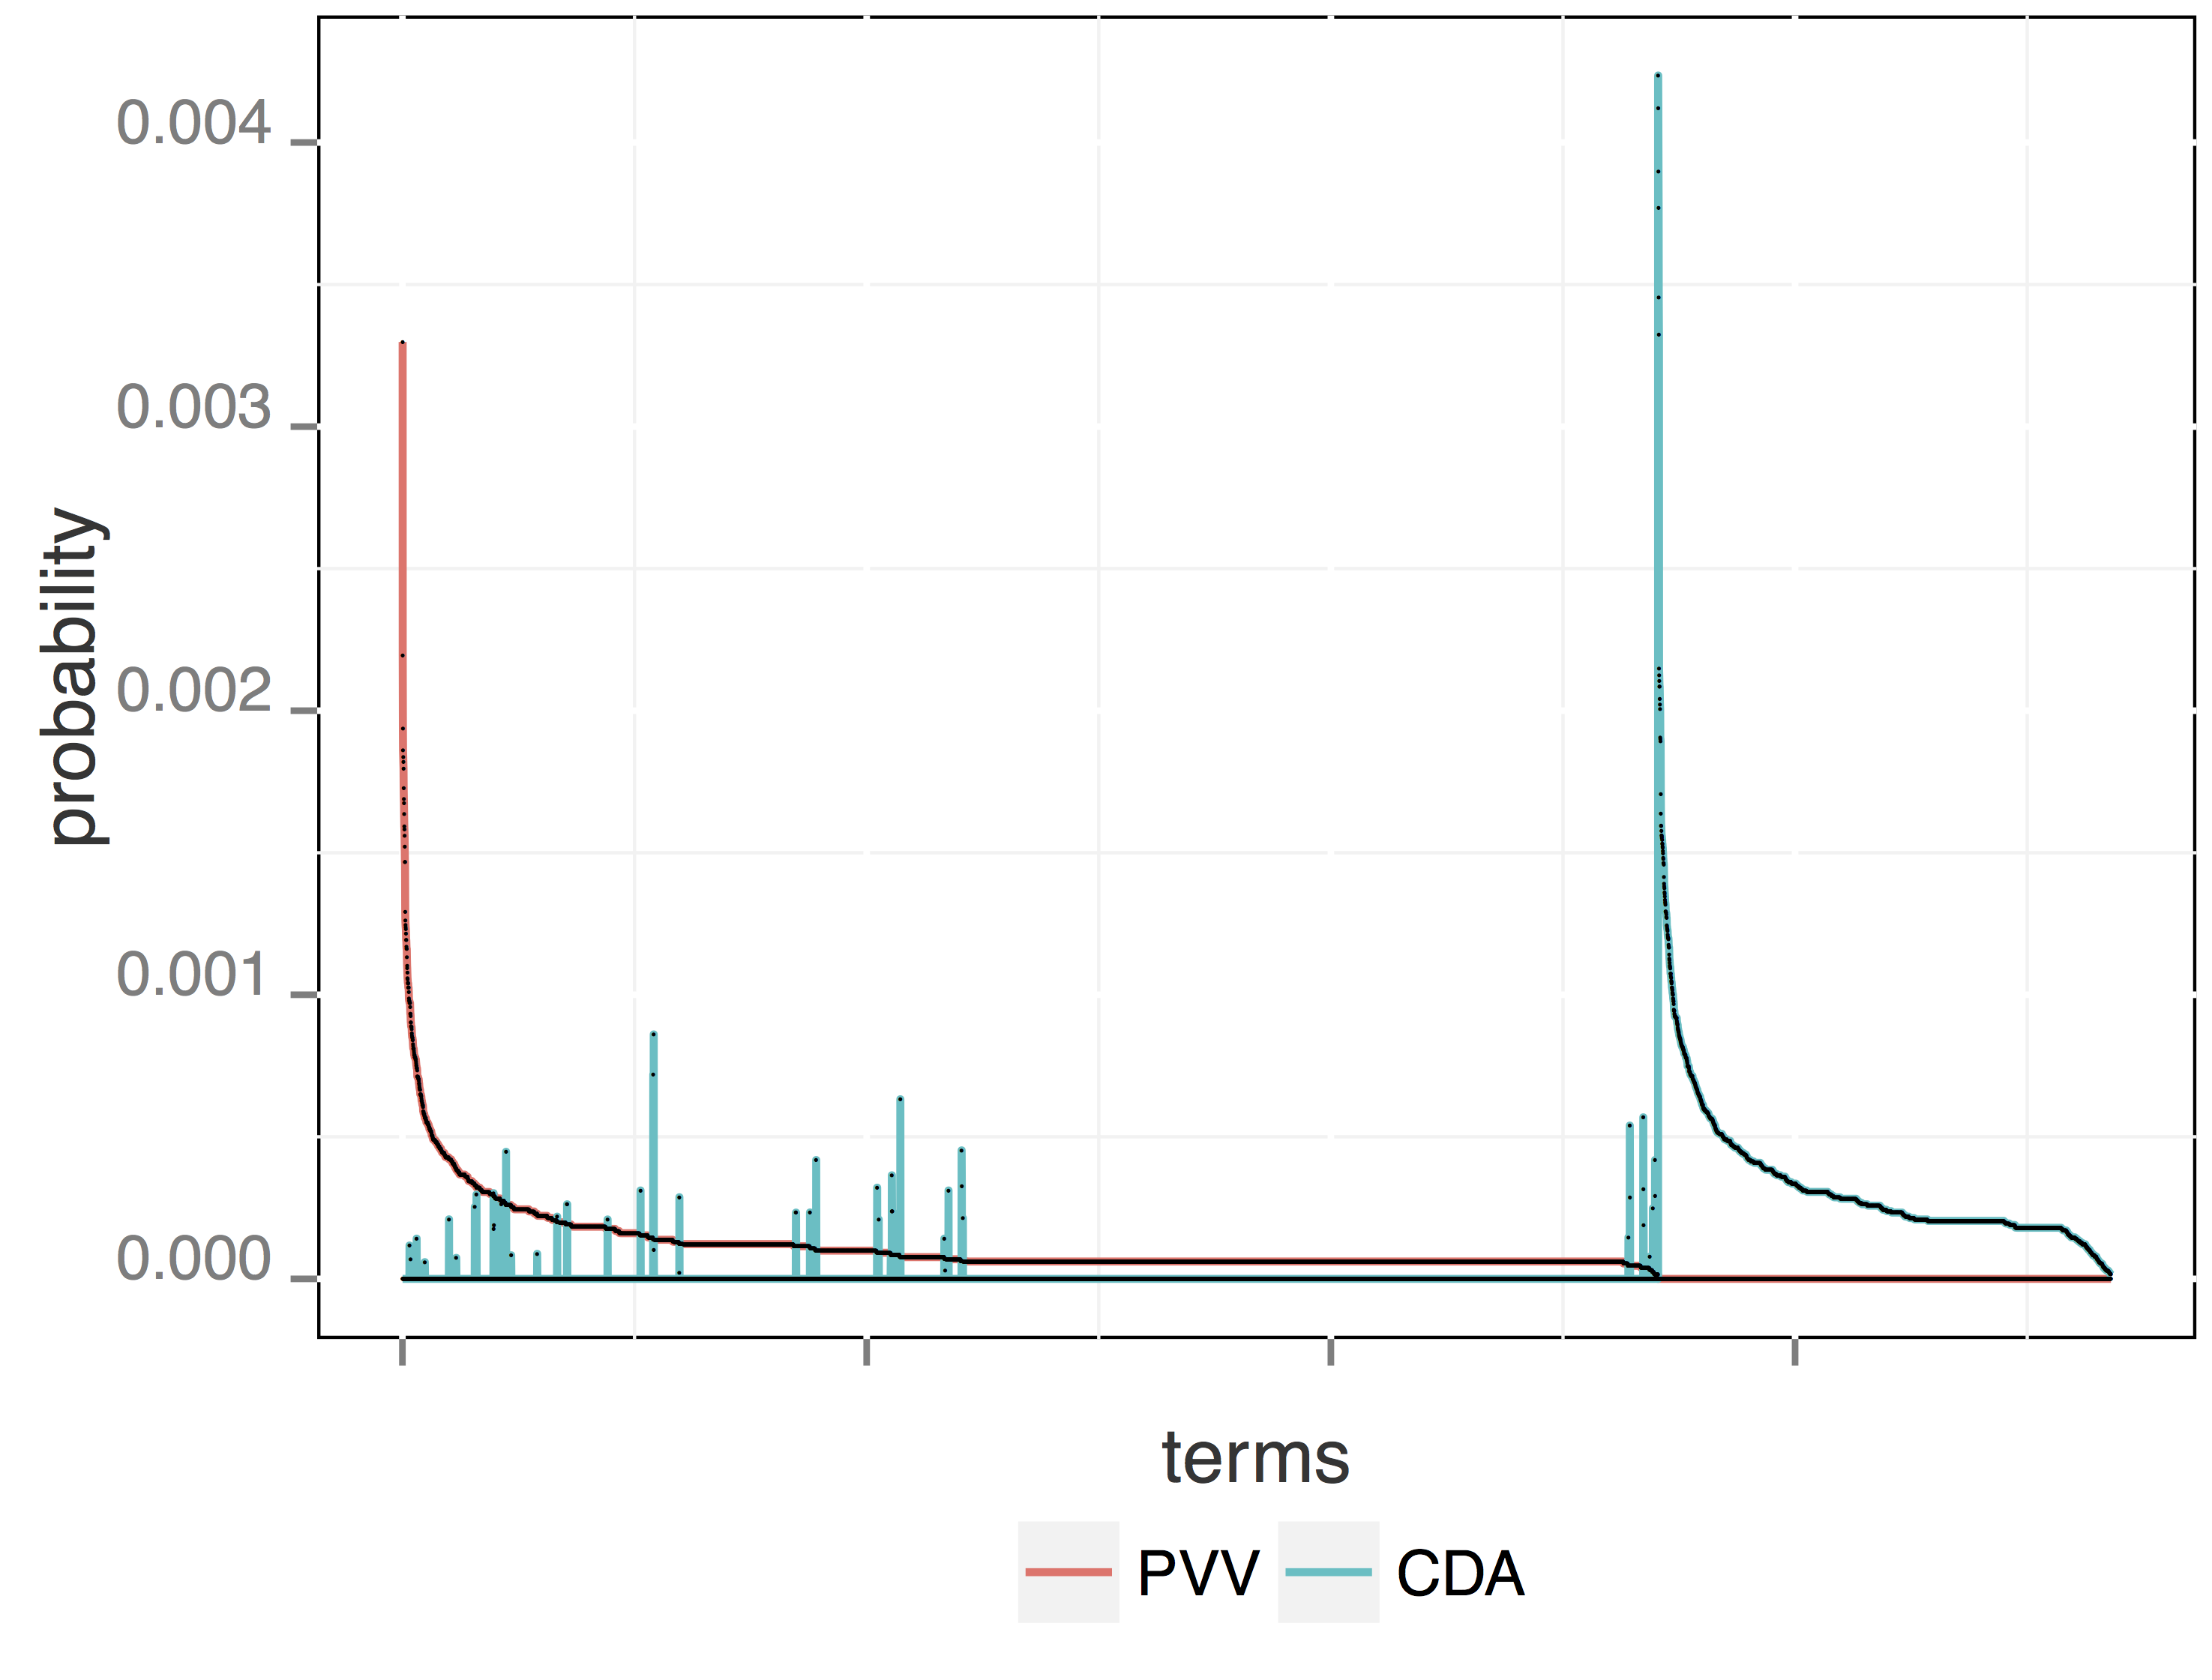
\includegraphics[width=\linewidth]{02-part-01/chapter-03/figs_and_tables/img_PVV-CDA.png}
\caption{\label{fig:HSPOO} \achswlm of two parties in opposition: Party for Freedom (PVV) and Christian Democratic Appeal (CDA)}
        \end{subfigure}
        ~ 
        \begin{subfigure}[b]{0.32\textwidth}
\centering
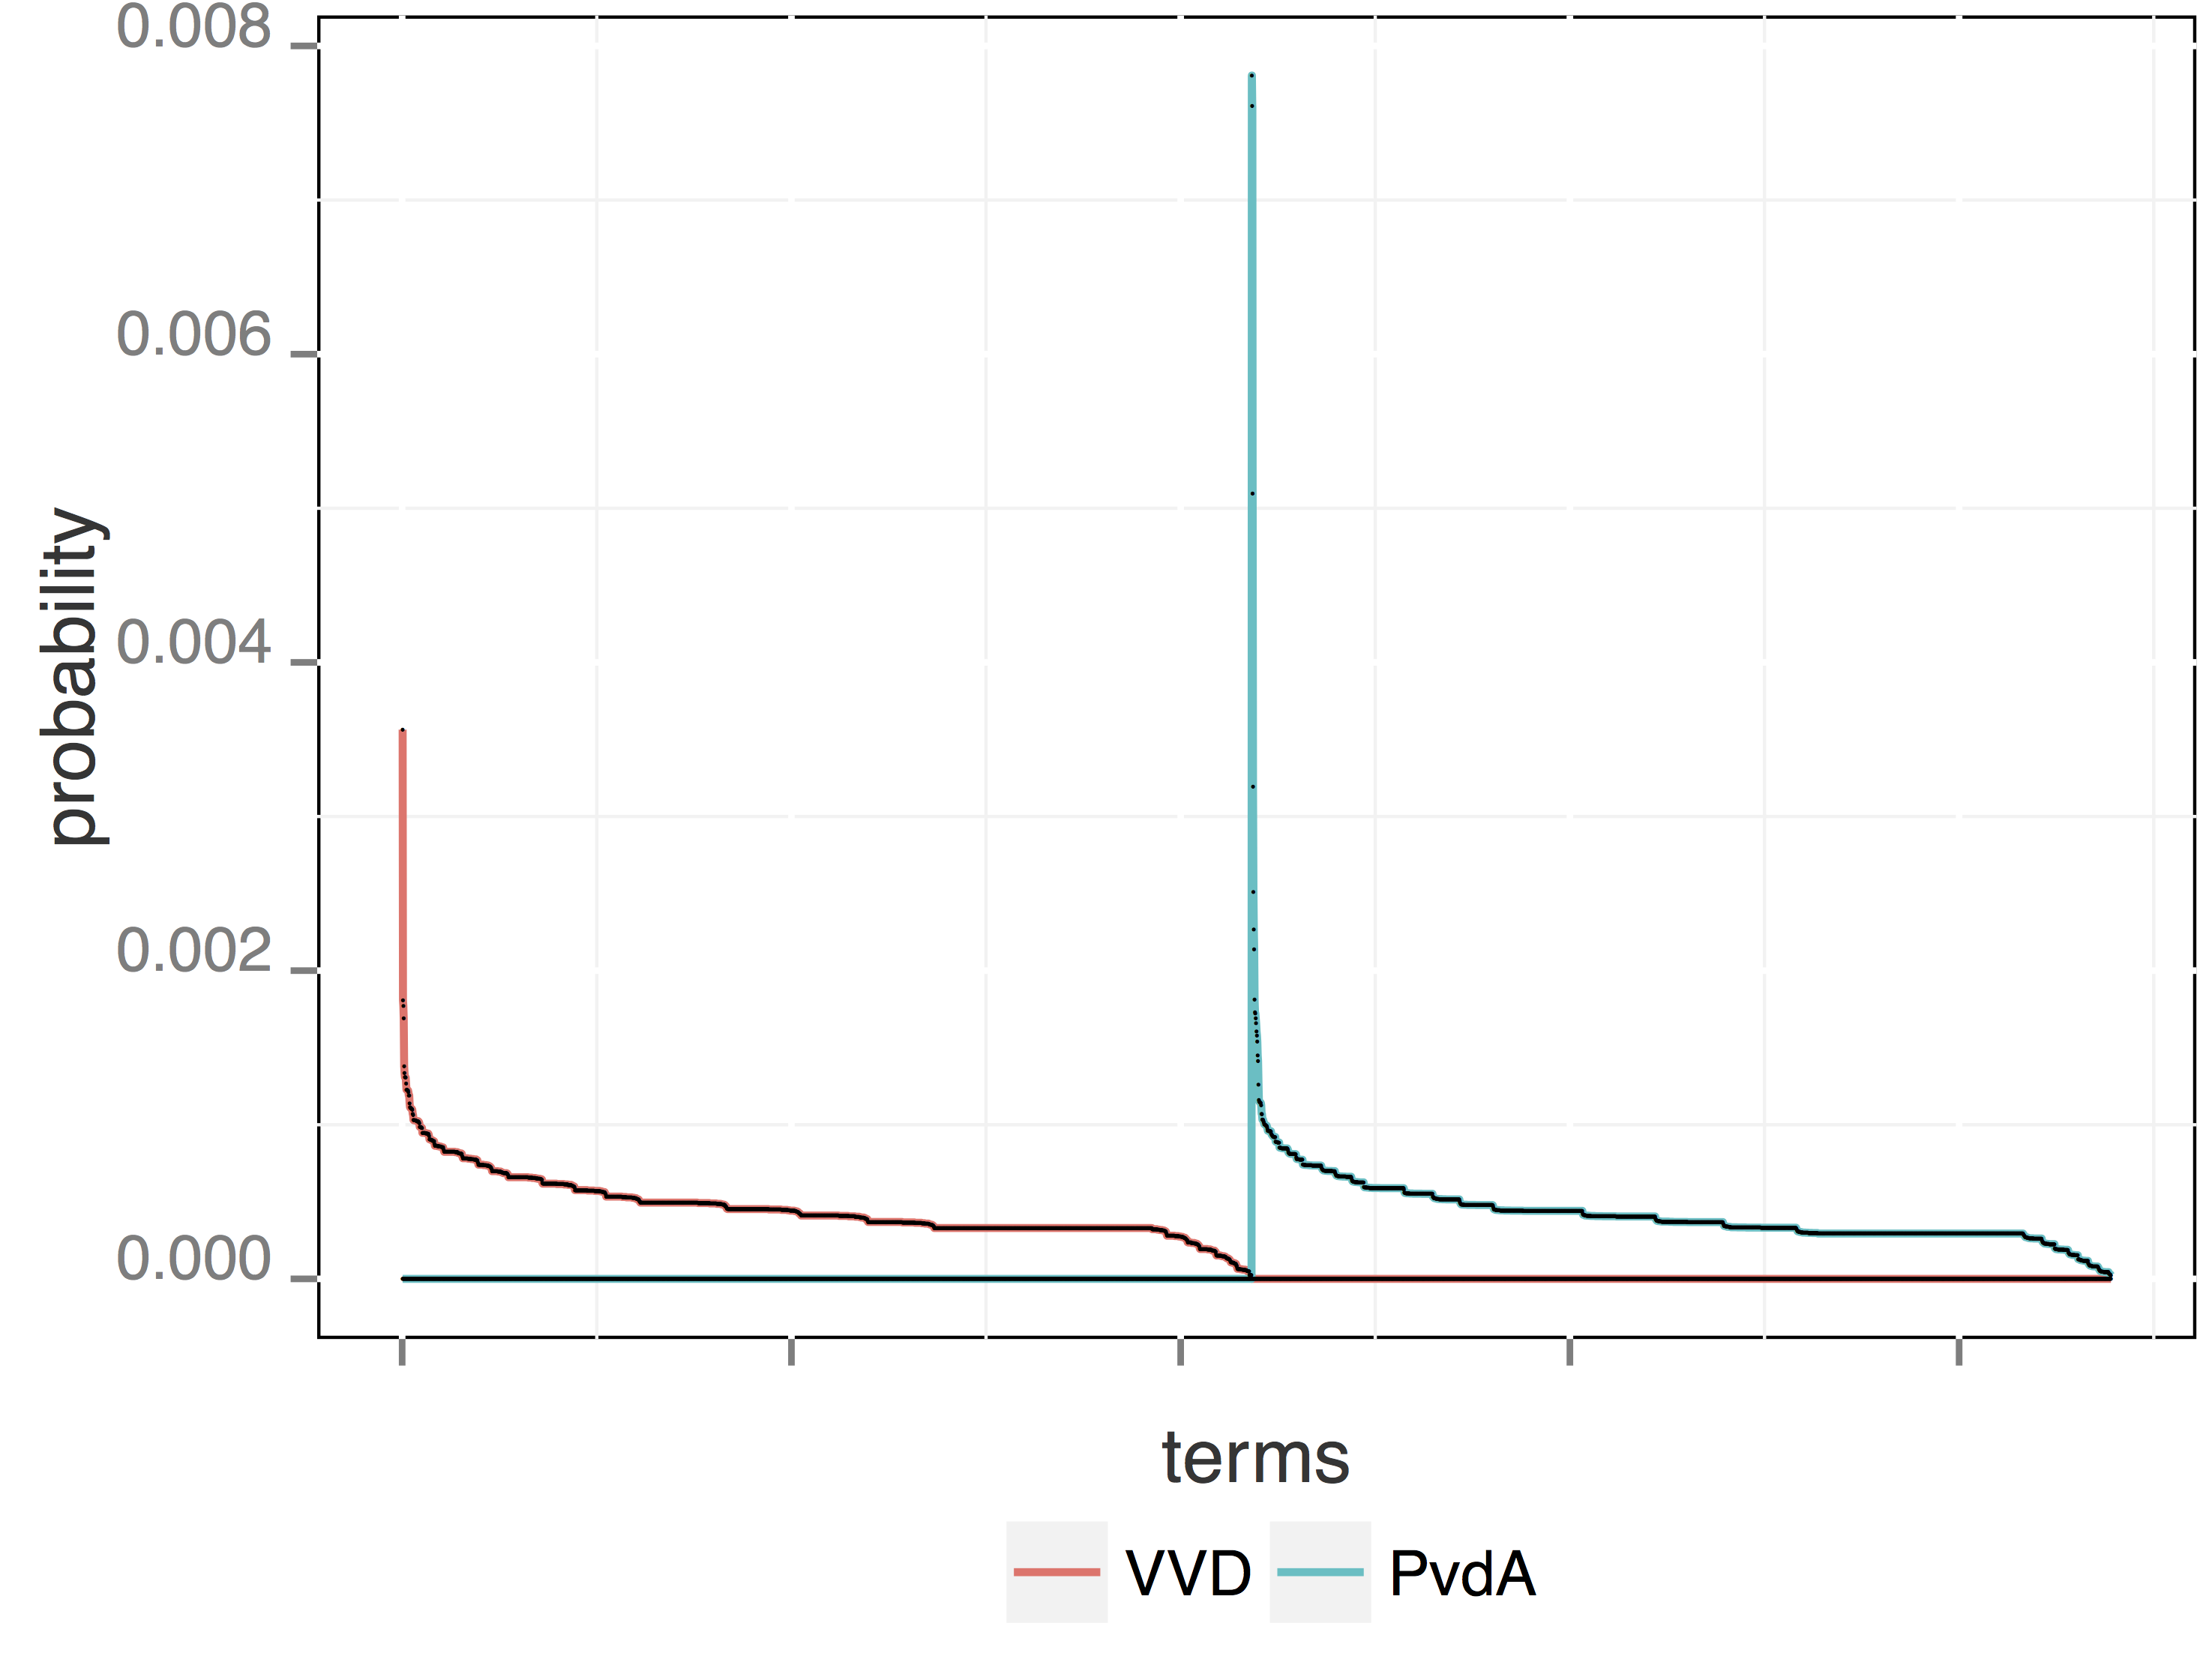
\includegraphics[width=\linewidth]{02-part-01/chapter-03/figs_and_tables/img_VVD-PvdA.png}
\caption{\label{fig:HSPCC} \achswlm of two parties in government: People's Party for Freedom (VVD) and Labour Party (PvdA)}
        \end{subfigure}
        \caption{\label{fig:HSP-pairs} \emph{Horizontal Separability}: probability distribution over terms based on \hswlms in party layer}
\end{figure}

In order to illustrate the vertical separability of \achswlm, we choose two different branches in the hierarchy: one from the leader of one of the opposition parties to the root, and the other from the leader of one of the government parties to the root. Figures \ref{fig:VSO} and \ref{fig:VSC} show probability distributions over words based on \achswlm of all entities in these two branches. They demonstrate that using \achswlm, we can decompose distribution over all terms to the highly separable distributions, each one representing the language usage related to the meaning behind the layer of the entity in the hierarchy. 

\begin{figure}[!t]
        \centering
        \begin{subfigure}[b]{0.45\textwidth}
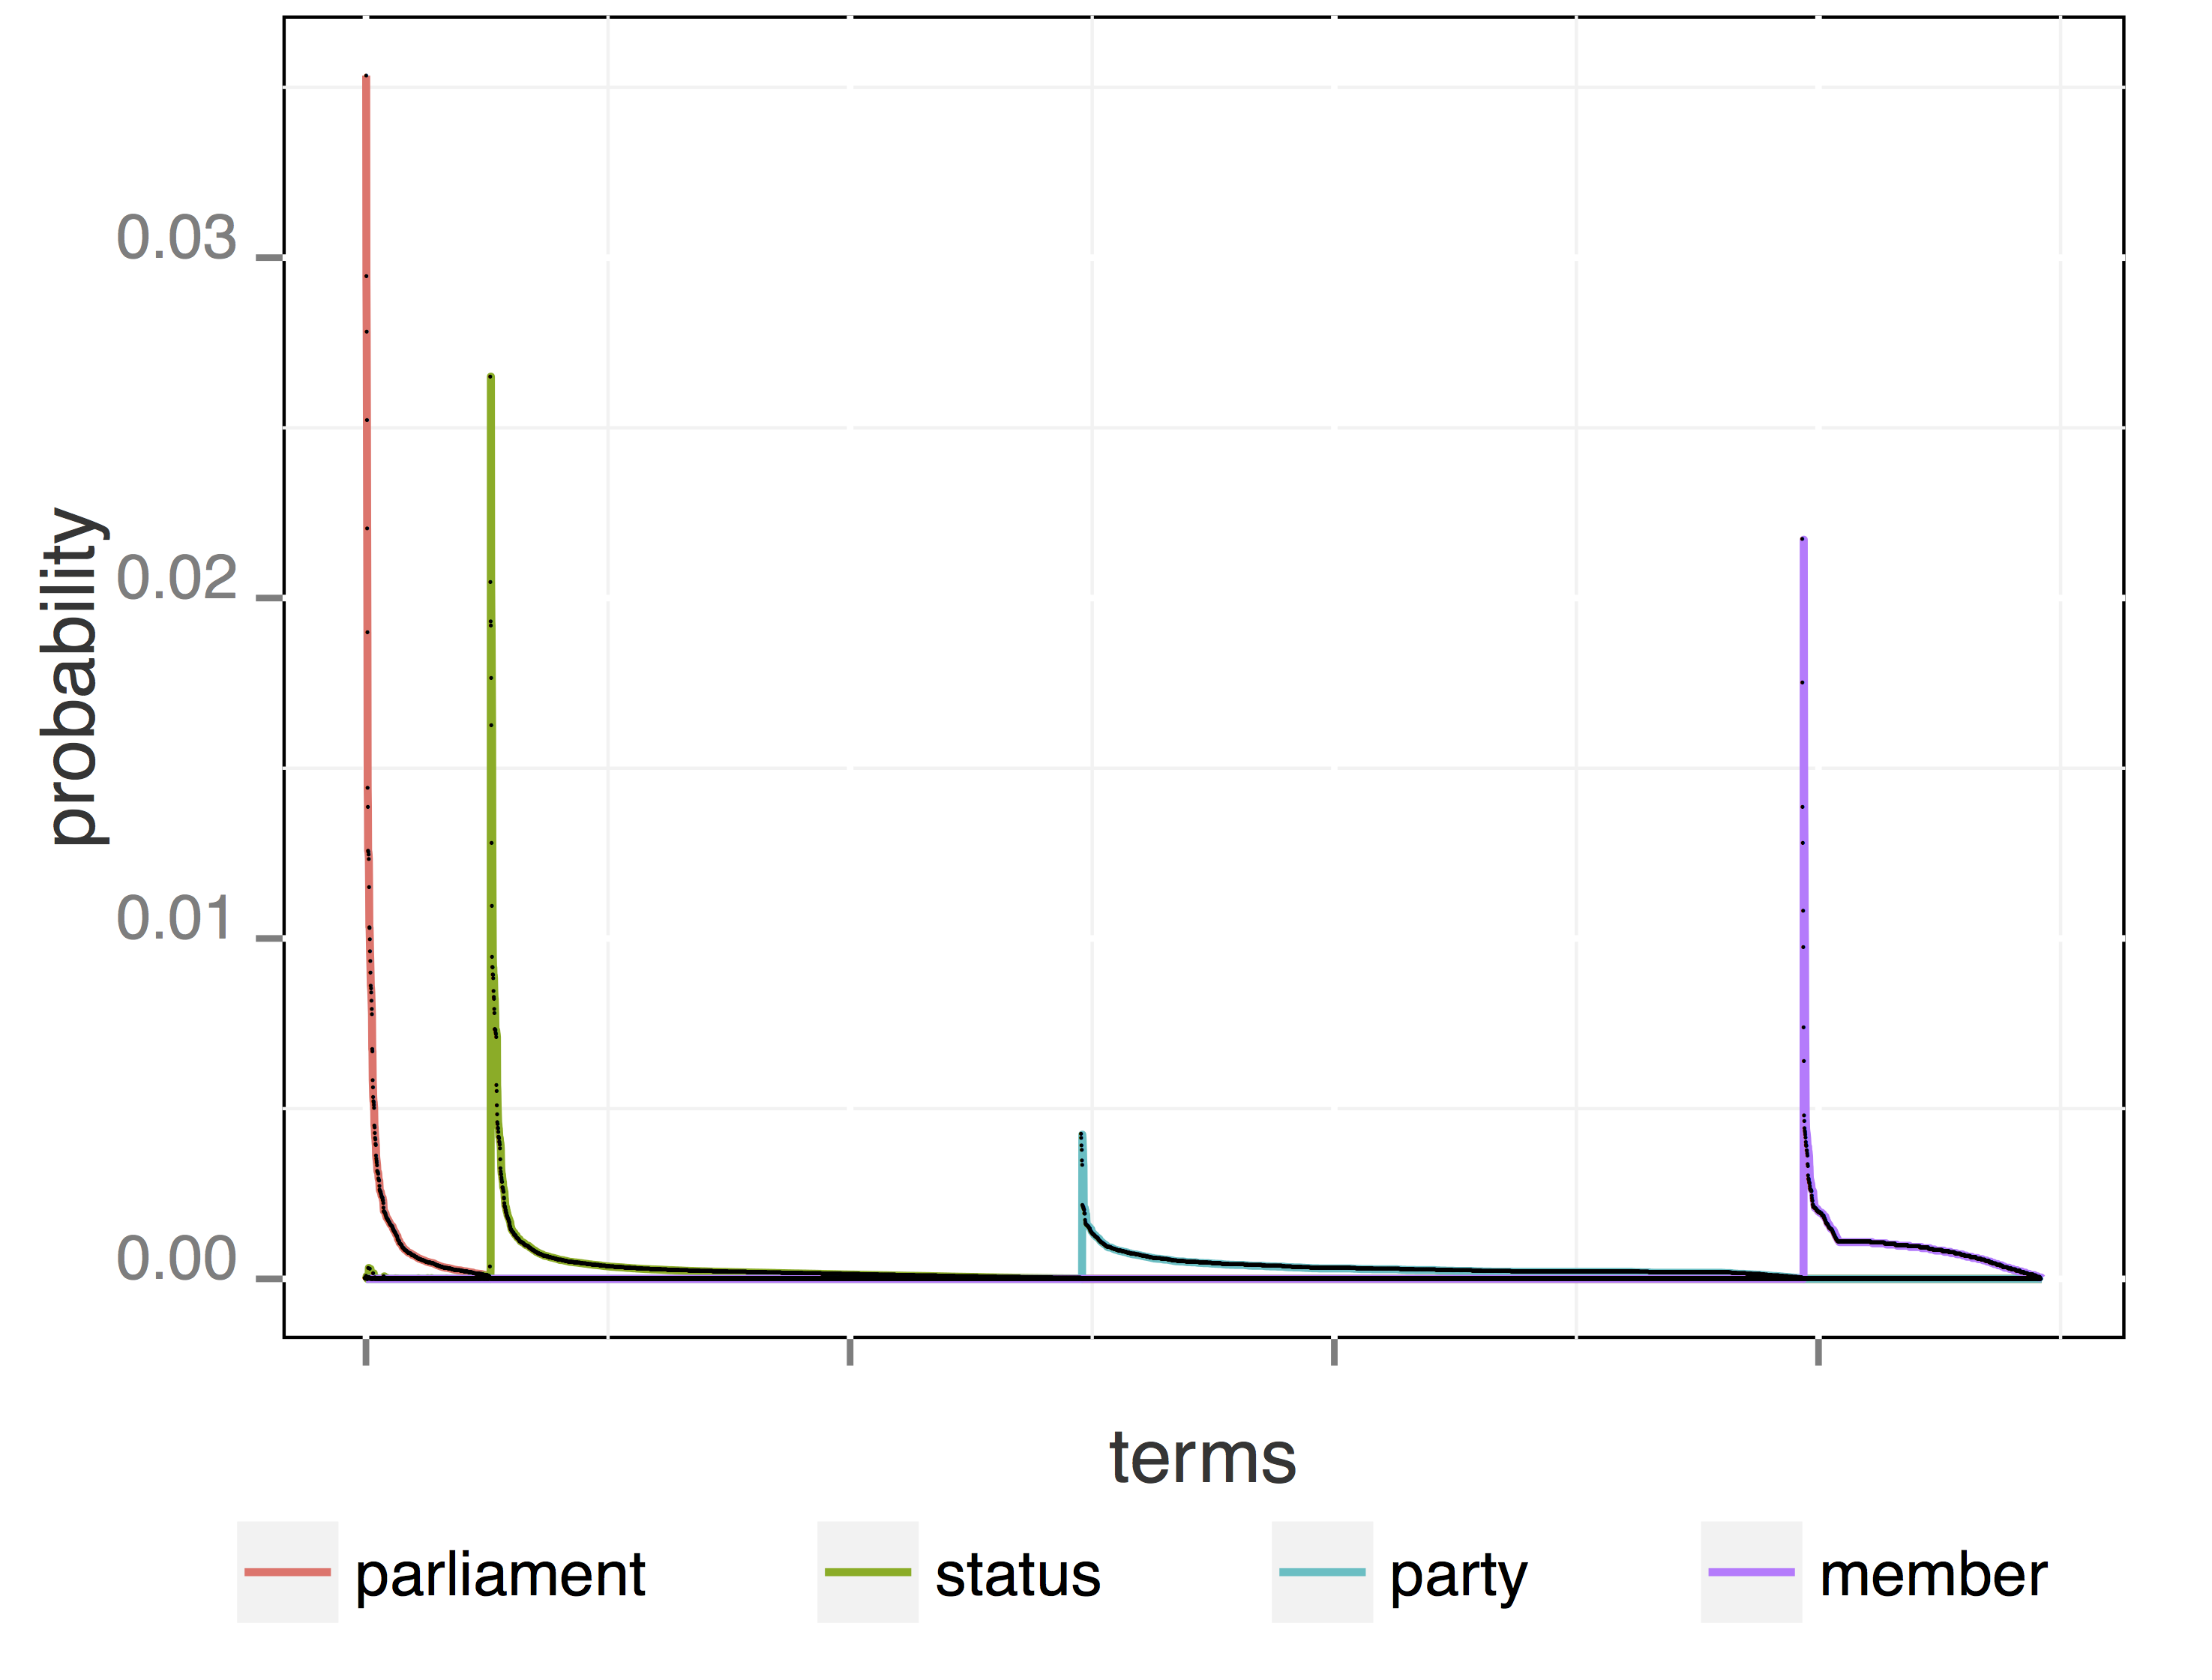
\includegraphics[width=\linewidth]{02-part-01/chapter-03/figs_and_tables/img_nlm02316.png}
\caption{\label{fig:VSO} \achswlm of S. van Haersma Buma (as the member of parliament - Leader of CDA), Christian Democratic Appeal (as the party), Opposition (as the status), and the Parliament}
        \end{subfigure}
        ~~~~~~~~
        \begin{subfigure}[b]{0.45\textwidth}
\centering
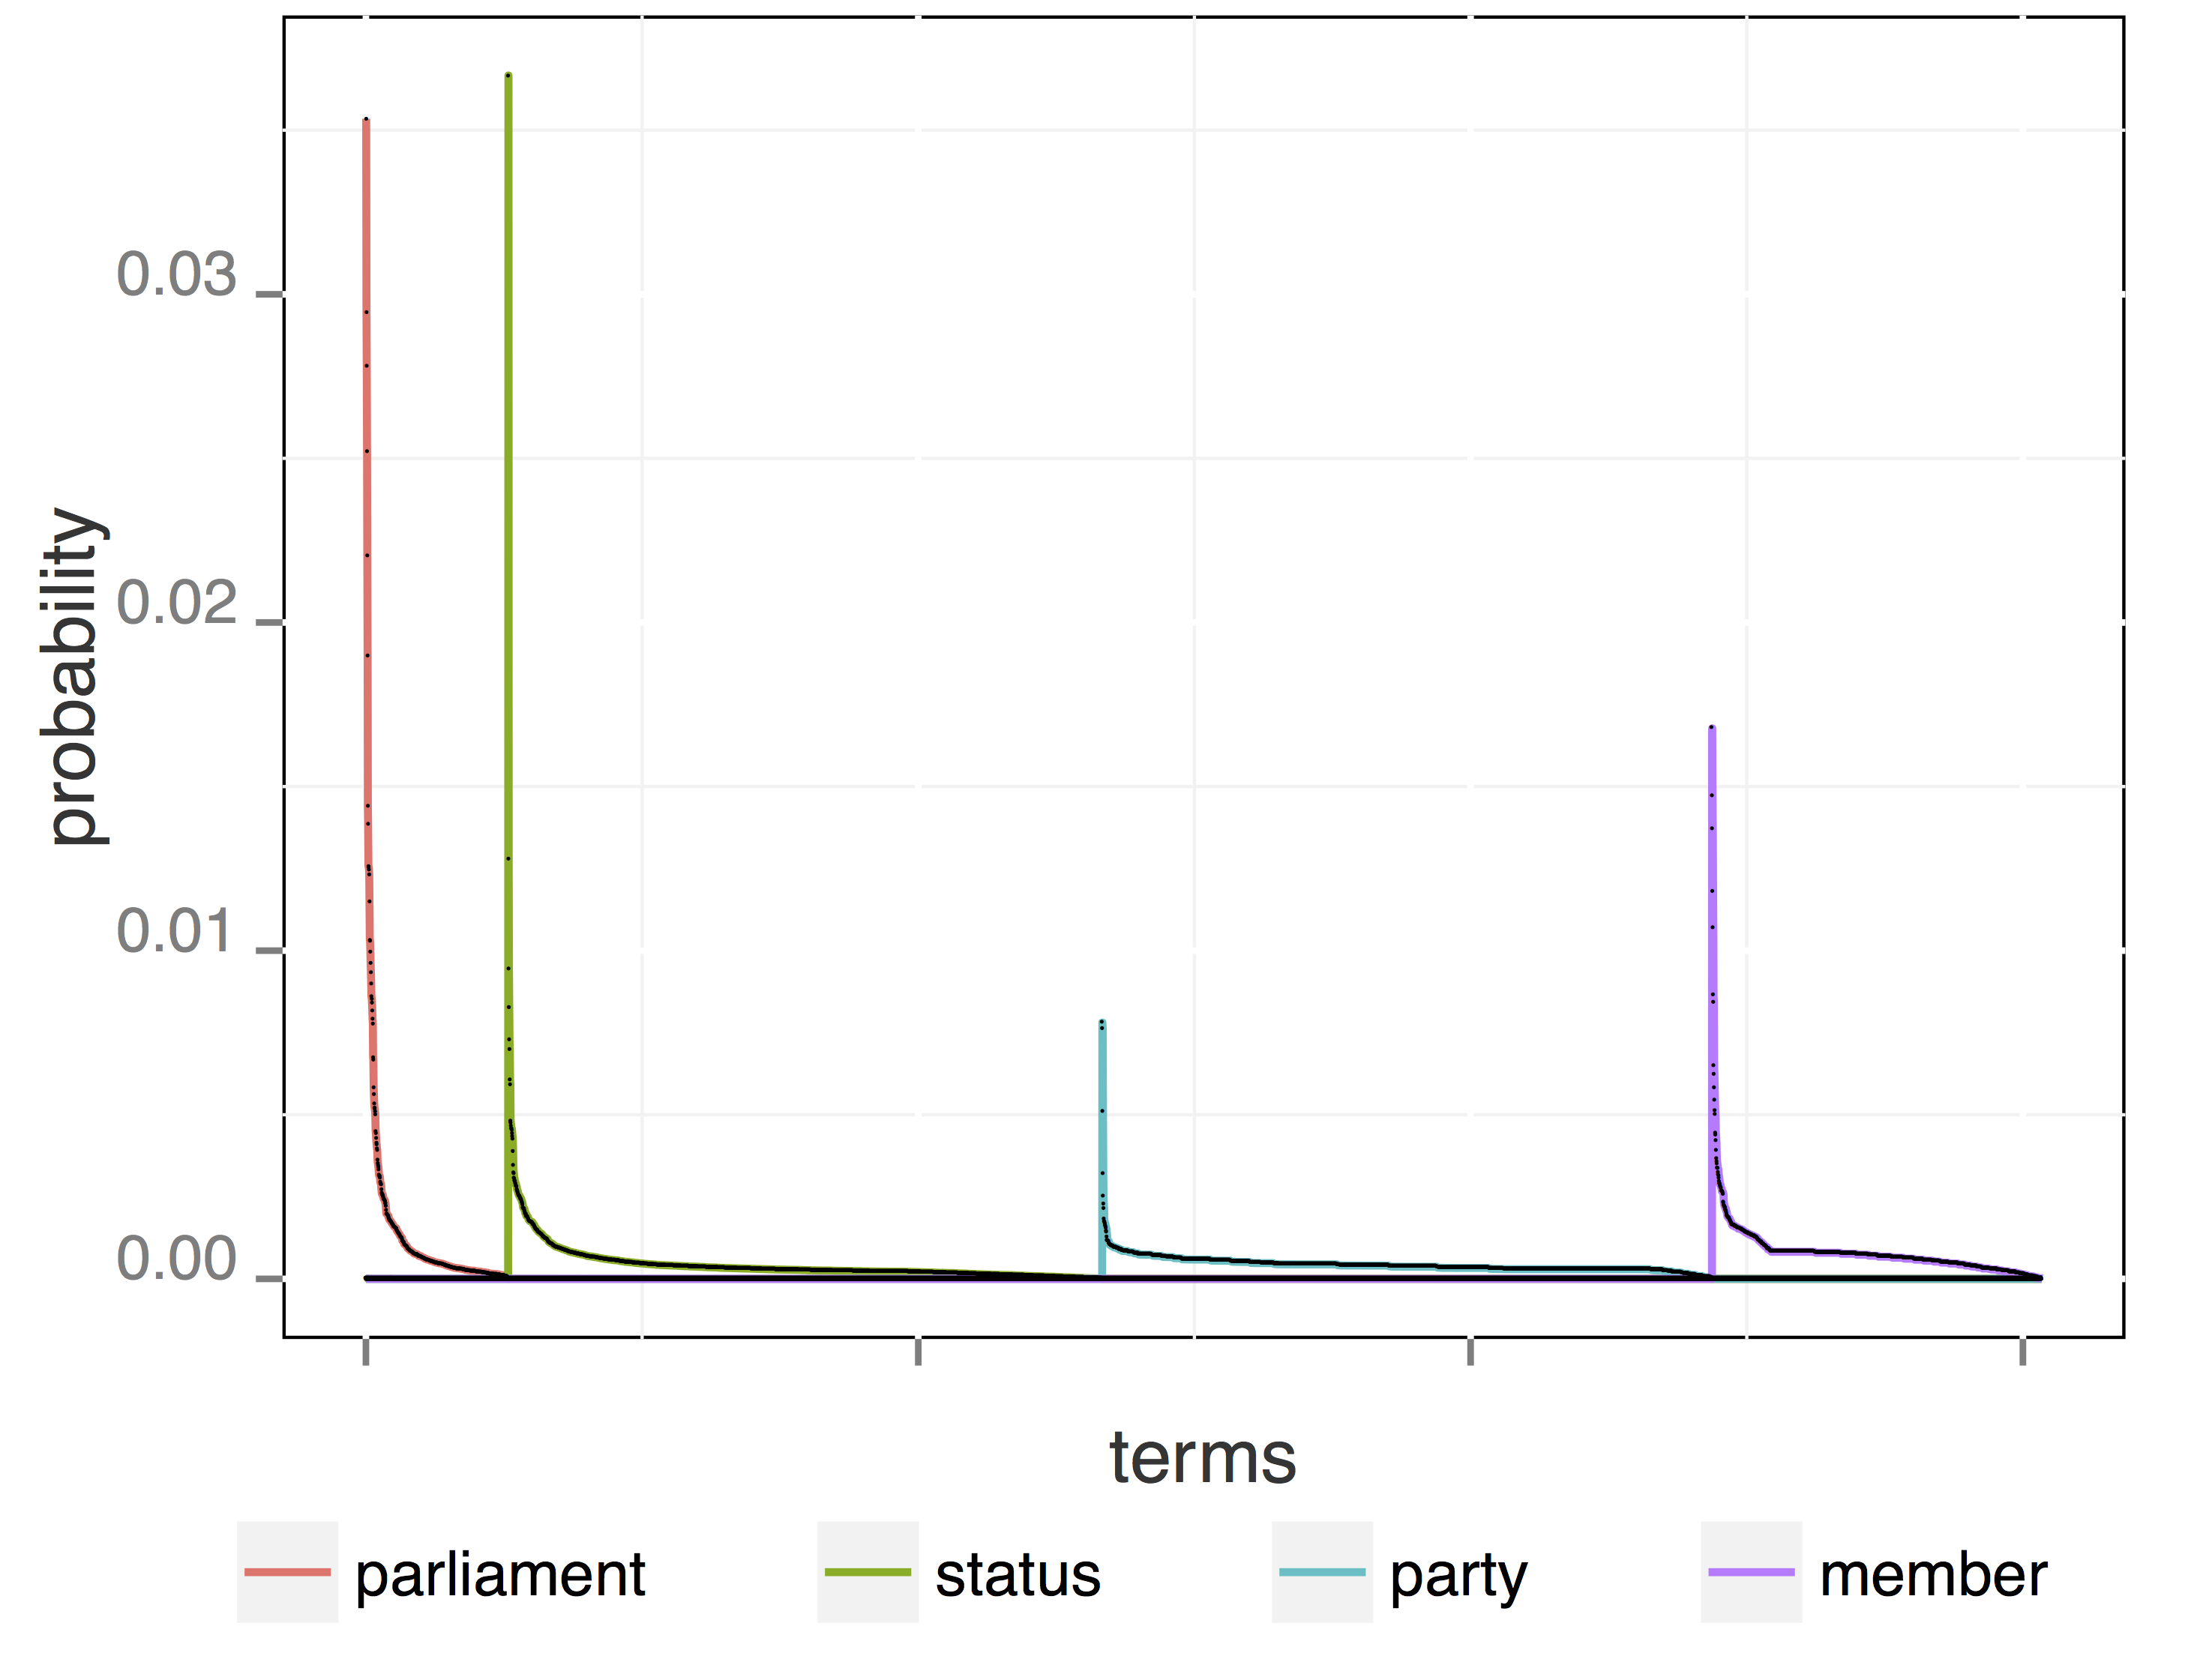
\includegraphics[width=\linewidth]{02-part-01/chapter-03/figs_and_tables/img_nlm02335.png}
\caption{\label{fig:VSC} \achswlm of D. Samson (as the member of parliament - Leader of PvdA), Labour Party (as the party), Government (as the status), and the Parliament}
        \end{subfigure}
        \caption{\label{fig:VS} \emph{Vertical Separability}: probability distribution over terms in different layers based on \hswlms in complete paths from the root to the terminal entities in the hierarchy}
\end{figure}

Two-dimensional separation property of \achswlm in the hierarchy is essentially due to the parsimonization effect in two directions. 
Intuitively, the horizontal separability is mainly the result of the specification stage. For example, when an entity is parsimonized given its direct parent, since the data in its parent is formed by pooling the data from the entity and its siblings, parsimonization makes the model of the entity separable from its siblings, which provide \emph{horizontal separation} in the resulting language models. On the other hand, vertical separability is mainly due to the generalization stage (and implicitly specification). For example, when an entity is parsimonized given its children, since they are specified already, parsimonization gets rid of the specific terms of the lower layer from the entity's model.


%---------------------------------------
\subsection{Separability for Transferability}
\label{subsec:Separability}
%---------------------------------------
As an extrinsic evaluation of the \hswlms, we investigate the effectiveness of the learned representations in a classification task in the parliamentary dataset with an evolving hierarchical structure. The task is to predict either the party that a member of the parliament belongs to, or the status of the member's party, having all the speeches given by that member in a period,  as well as all the speeches given by the members of all parties in a different period of parliament.

In the parliament, the composition of parties and statuses changes over different periods (Figure~\ref{fig:DutchParl}) and hence the speeches related to different entities can vary dramatically.  Due to this fact, cross-period classification is notoriously challenging \citep{Hirst:2014,yu:2008}.  We show that representing entities with \achswlm tackles the problem of having non-stable models when the composition of parliament evolves during the time, by capturing the essence of language models of parliamentary entities at aggregate levels. 

We use SVM as the base classifier and use the standard SVM as well as a SVM for training which we consider probabilities of terms in \achswlm as the weights of features in order to evaluate the effectiveness of \achswlm. Using the probabilities estimated by \achswlm as weights for features can be considered as a feature selection approach that filters out features that are not essential in accordance to the hierarchical position of entities and make the data representation more robust by taking out non-stable terms\footnote{We have also tried SVM along with a feature selection methods~\citep{Forman:2003,brank:2002} that uses the Information Gain (IG) to select features as a baselines and reported the results in~\citep{Dehghani:2016:ICTIR}.}.
We have employed conventional 5-fold cross validation for training and testing and to maintain comparability, we have used the same split for folding in all the experiments.

\input{02-part-01/chapter-03/figs_and_tables/table_corss_period_status.tex}

\input{02-part-01/chapter-03/figs_and_tables/table_corss_perios_party.tex}

Tables~\ref{tbl:swlm-status} and~\ref{tbl:swlm-party} show the performance of employing \acswlm on status and party classification respectively. 
Tables~\ref{tbl:SVM-status} and~\ref{tbl:SVM-party} indicate the results of SVM classifier on status and party classification respectively. Comparing the results in Tables~\ref{tbl:swlm-status} and~\ref{tbl:SVM-status}, we see that the accuracy of SVM in within period experiments is sometimes slightly better, but in cross period experiments, the classifier which uses \acswlm of statuses achieves better results.  This is also observed in the results in Table~\ref{tbl:swlm-party} compare to the results in Table~\ref{tbl:SVM-party}. 
%

For party classification, employing \acswlm results in a more significant improvement over the baseline.  \citet{Hirst:2014} discuss that since the status of members in parliament, compared to their party, has more effect on the content of their speeches, classifiers tend to pick features related to the status, not the party ideologies. So, SVM performs very well in terms of accuracy in the within-period experiments, but this performance is indebted to the separability of parties due to their status. Hence, changing the status in cross period experiments, using the trained model on other periods fails to predict the party, so the accuracies drop down. This is exactly the point which the strength of our proposed method kicks in. 
Since for each party, the \acswlm is less affected by the status of the party in that period, the model remains valid even when the status is changed.  In other words, eliminating the effect of the status layer in the party model in the specification stage ensures that the party model captures the essential terms related to the party ideology, not its status. Thereby, it is a stable model which is transferable through time.
%
We conducted the one-tailed t-test on the results. In both party and status classification, in all cases which \acswlm\ performs better than the SVM, the improvement is statistically significant ({p-value} $<$ 0.005).

To get a better intuition of the procedure of estimating \acswlm, consider the hierarchical relations of Dutch parliaments in the period of \emph{2006-2010} which is depicted in Figure~\ref{fig:DutchParl}. 
%
Assume that the goal is modeling language usage of ``Christian-Union (CU)'' as an entity in the party layer. In the speeches from the members of this party, words like ``\emph{Chairman}" or ``\emph{Agree}'' might occur repeatedly. However, they are not a good point of reference for the party's ideological language usage. In the procedure of estimating \acswlm\ of the "Christian-Union", these words are removed from the initial estimated standard language model in the specification stages, since ``\emph{Chairman}" is a general term in the parliamentary domain and is only able to explain the root entity and ``\emph{Agree}' is somehow an indicator of language usage of all the ``Government'' parties.
%
On the other side, consider the goal is to model language usage of ``Government'' as an entity in the status layer. Speeches from ``Christian-Union'' members, which are also counted as ``Government'' members, may contain words like ``\emph{Bible}'' or ``\emph{Charity}''.  It is trivial that involving these party-specific words in the constructed model for the ``Government'' in an individual period demolishes the comprehensiveness. In the procedure of estimating \acswlm\ for the ``Government'', in the generalization stages, these words are discarded from the model. This way, ``Government'' model does not lose its validity on other periods where the ``Christian-Union" is not in a Government party.

As another indicator of the effectiveness of \acswlm, it outperforms the SVM bringing all the data together from three different periods in both party and status classification. This is because it gets the chance of having richer train data which leads to more precise models. While in SVM, changes in the parliamentary composition make speeches diverse, and this makes it not to be able to learn a concrete model. 
\subsection{Invariance of the Representations}
\input{02-part-01/chapter-03/figs_and_tables/plot_cross_period_party_rep_divergence.tex}
As an intrinsic evaluation of the models, we evaluate the invariance of representations learned by our model over different periods---how similar are models of a particular in the hierarchy when trained on data from different periods. 
%
Since \achswlm is supposed to capture the essence of entities, not only \achswlm of an entity learned using an individual period should be valid for representing the entity on other periods, but also models of the same entity learned on data from different periods should be invariant. 

To assess this, we use the diversity of entities' models in different periods to measure their (in)variance over time.
%
First, all \achswlm from different periods of each party and each status is smoothed using Jelinek-Mercer smoothing \citep{Zhai:2001} considering all parliamentary speeches in the corresponding period as the background collection and with the same value of the smoothing parameter. Then, we use the Jensen-Shannon divergence as the diversity metric to measure dissimilarities between each two {\achswlm}s learned from different periods and then calculate the average of values for each entity. As the baseline, the same calculation is done for the standard language models of entities, i.e., language models estimated using maximum likelihood estimation. 
Figure~\ref{fig:cross_period_party_rep_divergence} shows the diversity of models in different periods.
%
As can be seen, in all entities in both party and status layers, diversity of \achswlm of different periods is lower than diversity of standard language models, which shows the extracted {\achswlm}s are more invariant over different periods. 


In order to better understand the results in the previous section, we zoomed in on the period of 2010-12 and 2012-2014 and looked into the confusion matrices of cross-period experiments and observed that most of the errors made by SVM are misclassifying members of CDA to PvdA and vice versa. These are the two parties that their statuses have been changed in these periods.  

\input{02-part-01/chapter-03/figs_and_tables/plot_cross_period_rep_divergence.tex}
We investigate representations of these two parties to understand how separation in the feature representation affects the performance of cross period classification. To do so, for each of these two classes, in each period, we extract three probability distributions on terms indicating their importance based on different weighting approaches: 1) Term Frequency (used as feature weights in SVM) and 2) probability of terms in \achswlm (used as feature weights in $SVM_{\achswlm}$). 
Then, as a metric to measure separability of features, we use the Jensen-Shannon divergence to calculate diversity of probability distributions in three cases: 1) Different Parties in the Same Period, 2) Same Party in Different Periods 3) Different Parties in Different Periods. 
To avoid the effect of the number of features on the value of divergence, we take the top 500 high scored terms of each of the weighting methods as the fixed length representatives of them. Figure~\ref{fig:cross_period_rep_divergence} shows the average diversity of distributions in each of the three cases for each of the three weighting methods.

As expected, the diversity of features for different parties in a same period is high for both methods. However, when we calculate the diversity of features for a same party in different periods, feature representations are different in  $TF$, which causes false negative errors in the classification of these two parties. An interesting observation is in the case of having different parties in different periods, while we have two different parties their feature representations are similar in $TF$, which leads to false positive errors in the classification. 

Considering these observations together reveals that SVM learns representations on the basis of features that are indicators of issues related to the status of parties, since they are the most discriminating terms considering one period and in within period experiments, the performance of SVM is indebted to the separability of parties based on their statuses. Hence, after changing the status in the cross period experiments, the trained model of the previous period generated by SVM fails to predict the accurate party.  In the same way, the status classifier is affected by different parties forming a government in different periods, leading to lower accuracies.   

This is exactly the point which the strengths of \achswlm kicks in. In fact, two-dimensional separability in the feature representation, enables $SVM_{\achswlm}$ to tackle the problem of having non-stable features in the model when the status of a party changes over time. In other words, eliminating the effect of the status layer in the party model, which is the result of the horizontal separation, ensures that the party model captures the terms related to the party ideology, not its status. Thereby, not only $SVM_{\achswlm}$ learns an effective model with acceptable accuracy in within period experiments, but also its learned models remain valid when the statuses of parties change. 

\section{Related Work}
This section discusses briefly the separation property in the related domains and review principles in information retrieval and text classification, which are associated with the concept of separability.  
In addition, some research on classification and topic modeling of hierarchical texts are discussed. 

Separability is a property which makes the data representation sufficient to distinguish instances and consequently enables autonomous systems to easily interpreter the data~\citep{Lewis:1992}. For instance in the classification task, classifiers learn more accurate data boundaries when they are provided with separable representations of data from different classes~\citep{Lewis:1995}. The importance of separability in classifiers has led to the fact that making data separable becomes part of classification. As the most familiar instances, SVM by adding extra dimensions implicitly transform the data into a new space where they are linearly separable~\citep{Burges:1998}.

Separation is also a pivoting concept in the information retrieval. Separating relevant from non-relevant documents is a fundamental issue in this domain~\citep{Robertson:1977,saracevic:1975,Lavrenko:2001}. In IR, separation plays more important role when instead of giving a rank list, a decision should be made about relevancy of documents, for example in the information filtering task~\citep{Lewis:1992}. As another instance, in the task of relevance feedback, there are some efforts on estimating a distinctive model for relevant documents so that it reflects not only  their similarity, but also their difference from whole collection, i.e., what makes them stand out or separated~\citep{Sparck:2003,Hiemstra:2004,Zhai:SMM:2001}. 

In this chapter, we address the separation property in the textual data that are organizable in a hierarchical structure. In a hierarchy, due to the existence of dependencies between entities, estimating separated models is a complex task. There is a range of work on the problem of hierarchical text classification~\citep{Sebastiani:2002, Sun:2001}, which tried to model hierarchical text-based entities. \citet{McCallum:1998} proposed a method for modeling an entity in the hierarchy which tackles the problem of data sparseness in lower layer entities. They used a shrinkage estimator to smooth the model of each leaf entity with the model of its ancestors to make the models more reliable. 
There is also similar research on XML data processing, as hierarchically structured data, which try to incorporate evidence from other layers as the context through mixing each element language models by its parent's models~\citep{sigurbjornsson:2004,ogilvie:2004}.
%Their method in fact balances a trade-off between specificity and reliability. Although estimates in the leaf entities are more specific, due to data sparseness in these entities, the estimations are less reliable. Further up the hierarchy, there are more data instances so estimates are more reliable but unspecific.
%
%Later, \citet{Oh:2011}, similar to \citeauthor{McCallum:1998} tried to involve global information beside the local entity data to estimate the model of the entity. However, concerning large scale hierarchies, their method dynamically controls the level of information that is needed to be gathered from ancestors.

Recently, \citet{Song:2014} tackled the problem of representing hierarchical entities with a lack of training data for the task of hierarchical classification.  In their work, given a collection of instances and a set of hierarchical labels, they tried to embed all entities in a semantic space, then they construct a semantic representation for them to be able to compute meaningful semantic similarity between them.
%
%By focusing on scalability, \citet{Gopal:2013}, presented a framework which uses regularization technique for classifying entities with hierarchical and graphical dependencies to handle training data sparseness. They considered that the nearby entities in the hierarchy share similar model parameters and recursively push the parameters of the model of a node to be similar to its parents. This way, they encourage models of siblings to be similar to each other. 
%Again, their goal is to leverage information across the hierarchy that could be beneficial in case of training data sparseness. 

\citet{Zhou:2011} proposed a method that directly tackles the difficulty of modeling similar entities at lower levels of the hierarchy. They used regularization so that the model of lower level entities have the same general properties as their ancestors, in addition to some more specific properties. 
%
Although these methods tried to model hierarchical texts, but their concerns were not making the models separable. Instead, they mostly addressed the problem of \emph{training data sparseness} \cite{Ha-Thuc:2011,Song:2014,McCallum:1998} or presenting techniques for \emph{handling large scale data} \cite{Gopal:2013,Oh:2011,Xue:2008,Ha-Thuc:2011}.

In terms of modeling hierarchical entities, \citet{Kim:2013} used Hierarchical Dirichlet Process \citep[HDP,][]{Teh:2006} to construct models for entities in the hierarchies using their own models as well as the models of their ancestors.  Also, \citet{Zavitsanos:2011} used HDP to construct the model of entities in a hierarchy employing the models of its descendants. This research tries to bring out precise topic models using structure of the hierarchy, but they do not aim to estimate separable models.  

As we discussed in Section~\ref{subsec:Separability}, our proposed approach can be employed as a feature selection method for text classification. Prior research on feature selection for textual information~\citep{SIGIR-Workshop-2010,Forman:2003} tried to improve classification accuracy or computational efficiency, while our method aims to provide a separable representation of data that helps train a transferable model. 
Apart from considering the hierarchical structure, our goals also differ from prior research on transferability of models. For instance, research on constructing dynamic models for data streams~\citep{Yao:2009,Blei:2006} first discovered the topics from data and then tried to efficiently update the models as data changes over the time, while our method aims to identify tiny precise models that are more robust and remain valid over time.  Research on domain adaptation~\citep{Xue:2008:plsa,Chen:2011} also tried to tackle the problem of missing features when very different vocabulary are used in test and training data.  This differs from our approach considering the hierarchical relations, as we aim to estimate separable models that are robust against changes in the structure of entities relations, rather than changes in the corpus vocabulary.


\section{Conclusion}
Building conceptually accurate models of data with a structure consisting of multiple layers, or a hierarchy, prompts us to analyse them at different abstraction levels.  However, this requires the ability to estimate separable models for hierarchical entities which capture their essential features taking into account their relative position in the hierarchy. 

In this chapter, we demonstrated that based on the ranking and classification principles, the \emph{separation property} in the data representation is a desirable foundational property which leads to separability of scores and consequently improves the accuracy of classifiers' decisions.  We stated this as the ``\ssp'' for optimizing expected effectiveness of classifiers.

We showed that in order to have horizontally and vertically separable models, they should capture all, and only, the essential terms of the entities taking their position in the hierarchy into account. Based on this, we introduced \hswlms for estimating separable models for hierarchical entities. We studied \achswlm and demonstrated that it offers separable distributions over terms for different entities both in case of being in the same layer or in different layers. 

We evaluated the performance of classification over time using separable representation of data and showed that separability makes the model more robust and transferable over time by filtering out non-essential non-stable terms.

% !TEX root = ../thesis-main.tex
\part{\titleof{p2-with-break}} % doesn't work!
\label{part2}
The unprecedented success of data-driven approaches has turned data into a first-class citizen in machine learning. Most of the times, the more data you have, the more accurate your model will be~\citep{halevy2009unreasonable,sun2017revisiting} and it is more crucial to provide massive amounts of training data when the models become more deep and complex.
Collecting such training sets by hand is often infeasible due to the time and expense of labeling data. Besides, hand-labeled training sets are static and we might need complete relabeling for instance when the modeling goals changes. Thus moving beyond fully supervised learning, like adapting weak supervision with the hope of overcoming the poverty of stimulus, is a key direction in machine learning research.

Humans can learn effortlessly from weak and inconsistent signals. However, it seems difficult to build fault-tolerant machine learning systems that learn, while even imperfect signals can contain a great deal of valid information.
Given the fact that only a tiny portion of real word applications operate on perfect condition, an essential aspect of any practical learning algorithm is the need to learn from inconsistent data provided by different sensors, noisy or weak supervision, and even when crucial information is missing from the supervision signal.

In Part~\ref{part2} of this thesis, we address the following research question:
\resq{p2}

The imperfect examples can come from labels provided by non-expert crowd workers, be the output of other models that are weaker (for instance with low accuracy or coverage), biased, or models trained on data from different related domains. 
Here in this part, we aim to study how the human can supervise machine learning systems, by labeling training data programmatically instead of labeling by hand. Then, given a vast amount of pragmatically generated labeled data, and maybe a small set of examples with true labels,  we discuss how to design neural networks that leverage the full capacity of the information in the data and go beyond the imperfection in the weakly annotated data.


In the first chapter of this part, Chapter~\ref{chap:4}, we address the following research question:
\resq{c4}

In this chapter, we propose to train a neural ranking model using weak labels that are obtained automatically without human annotators or any external resources (e.g., click data). We train a set of simple yet effective neural ranking models and study their effectiveness under various learning scenarios, i.e. point-wise and pair-wise, different objective functions, and using different input representations, from using a set of engineered features to encoding query/document using word embedding~\citep{Dehghani:2017:SIGIR}. We also discuss how privacy preserving approaches can benefit from models that are capable of learning from weak signals, where instead of labels from the original sensitive training data a noisy version is provided~\citep{dehghani:2017:neuir}.

Then, in the second chapter of this part, Chapter~\ref{chap:5} we focus on the following research question:
\resq{c5}

In this chapter we introduce \emph{Learning with Controlled Weak Supervision (\cws)}~\cite{Dehghani:2017:nips_metalearn, Dehghani:2017avoiding} and \emph{Fidelity Weighted Learning (\fwl)}~\citep{dehghani:2018:ICLR}, two semi-supervised approaches for training neural networks, where we have a large set of data with weak labels and a small amount of data with true labels. 
%
In \cws we train two neural networks in a meta-learning setup: a \tnet, the learner and a \cnet, the meta-learner.  The \tnet is optimized to perform a given task and is trained using a large set of unlabeled data that are weakly annotated. We propose to control the magnitude of the gradient updates to the \tnet using the scores provided by the second \cnet, which is trained on a small amount of supervised data. Thus we avoid that the weight updates computed from noisy labels harm the quality of the \tnet model.
%
\fwl is a student-teacher approach in which we modulate the parameter updates to a \emph{student} network (trained on the task we care about) on a per-sample basis according to the posterior confidence of its label-quality estimated by a \emph{teacher} (who has access to the high-quality labels).  


We show that we can train a neural ranker using a heuristic labeling function as weak supervision signal and go beyond the performance of this weak annotator, merely by choosing right architecture and objective functions and discuss how this can benefit learning in a privacy-preserving setup.
Given a semi-supervised setup, we apply our introduced methods, \cws and \fwl, to a range of language understanding tasks and empirically verify that they improve over semi-supervised alternatives and speeds up the training process. 

\medskip

% \chapter{\titleof{c4}}
\label{chap:4}
%
\begin{quote}
In many applications, to overcome the training data scarcity, we can provide supervision signals for learning algorithms not by hand-labeling the data, but by pseudo-labeling the data programmatically. This way, we can generate a much larger training set with a fairly low cost. However, we need to design algorithms that are capable of learning from weakly annotated labels and going beyond the imperfection in pseudo-labels. 
\end{quote}
%
\section{Introduction}
Neural networks are making great progress in many tasks in computer vision~\citep{krizhevsky2012imagenet}, natural language processing~\citep{collobert2008unified}, and information retrieval~\citep{welling2005exponential}. However, these models are data hungry and their performance is strongly correlated with the amount of available labeled data, which is not always readily available and can be expensive to obtain. 

Looking into the research works done in this area, most of them target stable benchmark tasks where standard large-enough datasets exist to train neural networks. However, the labeled data become the scarce commodity when we stray slightly from these standard benchmark tasks toward the realm of real-world applications. In this chapter, we focus on one of our research questions:
\resq{c4}

We aim to study how human can supervise machine learning systems, by labeling training data programmatically instead of labeling by hand. Then, given a vast amount of pragmatically generated labeled data, we discuss how to design neural networks that can go beyond the imperfection in the weakly annotated data. We also study how the ability to learn from noisy signals can lead to better performance when we have intentionally added noise to the training signals in a privacy-preserving training setup.

\medskip
In this chapter, we mainly target the \emph{ranking task}, as one of the core IR problems, where despite the advances of neural network based methods in many other related tasks like reading comprehension, there has been a little progress, mainly due to the lack of a large scale public dataset with query-document pairs labeled by relevance. 

We propose to use a heuristic based ranking method to generate pseudo-labels for a large set of unlabeled query-document pairs to train a neural ranking model given these pseudo-labels as sort of weak annotations.  We tried different architectures, in terms of different objectives and different input representations and study how they learn the ranking task in weak supervision setup.

Interestingly, we observe that using just training data that are annotated by a weak annotator model as the weak annotator, we can outperform that weak annotator on the test data. Based on our analysis, the achieved performance is generally indebted to three main factors: 
%
First, defining an objective function that aims to learn the ranking instead of calibrated scoring to relax the network from fitting to the imperfections in the weakly supervised training data.
%
Second, letting the neural networks learn optimal query/document representations instead of feeding them with a representation based on predefined features. This is a key requirement to maximize the benefits from deep learning models with weak supervision as it enables them to generalize better.
%
Third and last, the weak supervision setting makes it possible to train the network on a massive amount of training data, which is crucial for learning representations.
%

We further thoroughly analyze the behavior of models to understand what they learn, what is the relationship among different models, and how much training data is needed to go beyond the weak supervision signal. We also study if employing deep neural networks may help in different situations.
%
We also examine the scenario of using the network trained on a weak supervision signal as a pre-training step. We demonstrate that, in the ranking problem, the performance of deep neural networks trained on a limited amount of supervised data significantly improves when they are initialized from a model pre-trained on weakly labeled data.

Finally, we study how a neural ranking model that learns from weak/noisy signals can be effectively employed in a setup that noise is intentionally added to the training signal to preserve privacy.


\subsection{Detailed Research Questions}
We break down our main research question in this chapter into three concrete research questions:
\begin{resqbox}
\begin{enumerate}
\item[\textbf{\resqname{c4.1}}] \emph{\resqcontent{c4.1}}
\item[\textbf{\resqname{c4.2}}] \emph{\resqcontent{c4.2}}
\item[\textbf{\resqname{c4.3}}] \emph{\resqcontent{c4.3}}
\end{enumerate}
\end{resqbox}
In the following sections, we will address these research questions.
\section{Weakly Supervised Neural Rankers}
\label{sec:weakly_supervised_neural_rankers}
Despite the promising performance from neural networks on many language understanding tasks, ranking has remained a challenging problem. Besides the inherent difficulty of ``assessing relevance'', the lack of availability of public large scaled datasets that consist query-document pairs annotated by relevance labels, makes it difficult to advance data hungry models for this task.

Therefore, it is essential to come up with solutions that let us train neural ranking models, where there is no labeled data it is only available at an extremely limited size. 
One the main idea to tackle this problem is to make use of weak human supervision or weakly labeled data, as it is much cheaper to collect or readily available at much larger scale. This section focuses on addressing the following questions:
\resq{c4.1}

We propose to pseudo-label a large set of unlabeled data using an unsupervised method and train a neural ranker using these ``weak'' or ``noisy'' labels. Given this setup, we examine various neural ranking models with different ranking architectures and objectives, i.e., point-wise and pair-wise, as well as different input representations, from encoding query-document pairs into dense\:/\:sparse vectors to learning query\:/\:document embedding representations. 

Our results have broad impact as the proposal to use unsupervised traditional methods as weak supervision signals and is applicable to a variety of IR tasks, such as filtering or classification, without the need for supervised data.  More generally, our approach unifies the classic IR models with currently emerging data-driven approaches in an elegant way.

\subsection{Pseudo-Labeling Unlabeled Data}
\label{sec:pseudo_labeling}
We use the idea of ``Pseudo-Labeling'' and propose to leverage a classic unsupervised IR model to annotate a large amount of unlabeled data and infer weak labels and use this signal to train supervised models as if we had the ground truth labels.
Since the data is generated programmatically, we can generate billions of training samples with almost no cost. 
\footnote{Weak supervision for training a ranker may refer to using click-through data. Here, we assume that no external information, e.g. search logs, is available.}

We focus on query-dependent ranking as a core IR task. To this aim, we take a well-performing existing unsupervised retrieval model, such as BM25. This model plays the role of ``pseudo-labeler'' in our learning scenario. In more detail, given a target collection and a large set of training queries (without relevance judgments), we make use of the pseudo-labeler to rank/score the documents for each query in the training query set. The goal is to train a ranking model given the scores/ranking generated by the pseudo-labeler as a weak supervision signal.

In the followings, we describe different neural architectures in details and finally investigate their effectiveness when trained on weakly annotated data.  

\subsection{Neural Ranking Architectures}
\label{sec:neural_ranking_arch}
In this section, we introduce three different neural ranking models that are trained based on different ``objectives''. We describe the architecture of the base neural network shared by these models. We further discuss the three different ``input layers'' used in our neural rankers to encode information of given query-document pairs.
\medskip

\label{sec:models}
\begin{figure}[t]
    \centering
    \begin{subfigure}[t]{0.26\columnwidth}
        \centering
        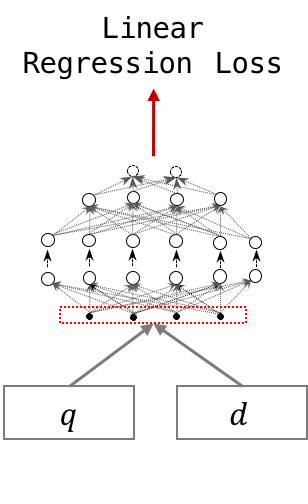
\includegraphics[height=5cm]{03-part-02/chapter-04/figs_and_tables/fig_model_1.png}%
        \caption{\label{fig:m1}\mone model}
    \end{subfigure}%
    ~
    \begin{subfigure}[t]{0.40\columnwidth}
        \centering
        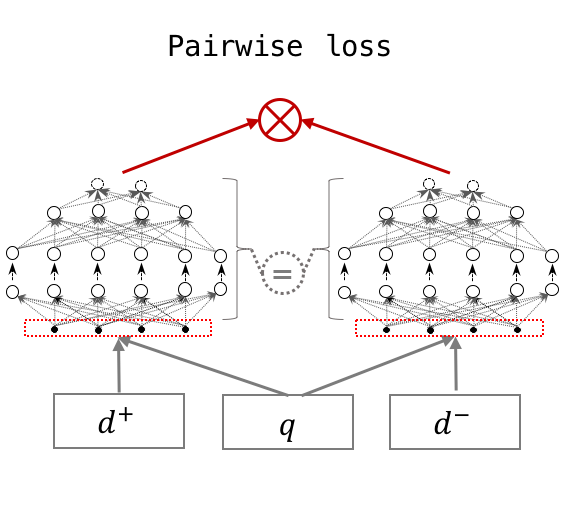
\includegraphics[height=5cm]{03-part-02/chapter-04/figs_and_tables/fig_model_2.png}%
        \caption{\label{fig:m2}\mtwo model}
    \end{subfigure}%
    ~
    \begin{subfigure}[t]{0.37\columnwidth}
        \centering
        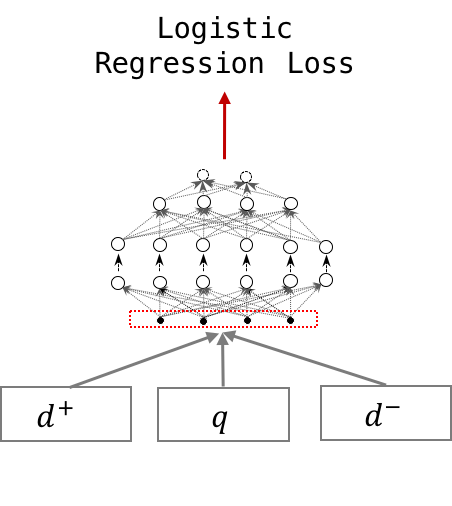
\includegraphics[height=5cm]{03-part-02/chapter-04/figs_and_tables/fig_model_3.png}%
        \caption{\label{fig:m3}\mthree model}
    \end{subfigure}%
    \caption{\label{fig:ranking-arch} Different ranking architectures.}
\end{figure}
%

We define three different ranking models, one point-wise and two pair-wise models:

\subsubsection{\label{sec:modelone}\Modelone}: This architecture models a point-wise ranking model that learns to predict retrieval scores for query-document pairs. More formally, the goal in this architecture is to learn a \emph{scoring function} $\mathcal{S}(q, d; \theta)$ that determines the retrieval score of document $d$ for query $q$, given a set of model parameters $\theta$.
%
In the training stage, we are given a training set comprising of training samples each a triple $x = (q,d, s_{q,d})$, where $q$ is a query from training query set $Q$, $d$ represents a retrieved document for the query $q$, and $s_{q,d}$ is the relevance score (calculated by a weak supervisor), which is acquired using a retrieval scoring function in our setup.
%
We consider the mean squared error as the loss function for a given batch of training samples:
\begin{equation}
\mathcal{L}(b; \theta) = \frac{1}{|b|} \sum_{i=1}^{|b|}{(\mathcal{S}(\{q, d\}_i; \theta) - s_{\{q, d\}_i})^2}
\end{equation}
where $\{q, d\}_i$ denotes the query and the corresponding retrieved document in the $i^{th}$ training sample, i.e., $x_i$ in the batch $b$.
The conceptual architecture of the model is illustrated in Figure~\ref{fig:m1}.


\subsubsection{\label{sec:modeltwo}\Modeltwo}:
In this model, similar to the previous one, the goal is to learn a scoring function $\mathcal{S}(q, d; \theta)$ for a given pair of query $q$ and document $d$ with the set of model parameters $\theta$. 
However, unlike the previous model, we do not aim to learn a calibrated scoring function. 
In this model, as it is depicted in Figure~\ref{fig:m2}, we use a pair-wise scenario during training in which we have two point-wise networks that share parameters and we update their parameters to minimize a pair-wise loss.
In this model, each training sample has five elements: $x = (q,d_1, d_2, s_{q,d_1}, s_{q,d_2})$.
During the inference, we treat the trained model as a point-wise scoring function to score query-document pairs.

We have tried different pair-wise loss functions and empirically found that the model learned based on the hinge loss (max-margin loss function) performs better than the others. 
Hinge loss is a linear loss that penalizes examples that violate the margin constraint. It is widely used in various learning to rank algorithms, such as Ranking SVM~\citep{Herbrich:1999}. The hinge loss function for a batch of training samples is defined as follows:
\begin{equation}
\begin{aligned}
\mathcal{L}(b; \theta) = \frac{1}{|b|}
\sum_{i=1}^{|b|}
\max\big\{
& 
0, \varepsilon - \text{sign}
(s_{\{q, d_1\}_i} - s_{\{q, d_2\}_i})
& \\ & 
\left(\mathcal{S}\left(\{q, d_1\}_i; \theta\right) -\mathcal{S}\left(\{q, d_2\}_i; \theta\right)\right)
\big\}
, 
%\nonumber
\end{aligned}     
\end{equation}
where $\varepsilon$ is the parameter determining the margin of hinge loss. We found that as we compress the outputs to the range of $[-1, 1]$, $\varepsilon=1$ works well as the margin for the hinge loss function.

\subsubsection{\label{sec:modelthree}\Modelthree}:
The third architecture is based on a pair-wise scenario during both training and inference (Figure~\ref{fig:m3}). This model learns a \emph{ranking function} $\mathcal{R}(q, d_1, d_2; \theta)$ which predicts the probability of document $d_1$ to be ranked higher than $d_2$ given $q$.
Similar to the \modeltwo, each training sample has five elements: $x = (q,d_1, d_2, s_{q,d_1}, s_{q,d_1})$.
For a given batch of training samples, we define our loss function based on cross-entropy as follows:
\begin{align}
\mathcal{L}(b; \theta) = -\frac{1}{|b|}
\sum_{i=1}^{|b|} &
P_{\{q,d_1,d_2\}_i} \log(\mathcal{R}(\{q,d_1,d_2\}_i; \theta)) \\
&
+ (1- P_{\{q,d_1,d_2\}_i})\log(1- \mathcal{R}(\{q,d_1,d_2\}_i; \theta)) \nonumber
\end{align}
where $P_{\{q,d_1,d_2\}_i}$ is the probability of document $d_1$ being ranked higher than $d_2$, based on the scores obtained from training sample $x_i$:
\begin{equation}
P_{\{q,d_1,d_2\}_i} = \frac{s_{\{q,d_1\}_i}}{s_{\{q,d_1\}_i} + s_{\{q,d_2\}_i}}
\end{equation}

A similar loss function has been previously used in RankNet~\citep{Burges:2005}. It is notable that at inference time, we need a scalar score for each document. Therefore, we need to turn the model's pair-wise predictions into a score per document. To do so, for each document, we calculate the average of predictions against all other candidate documents, which has $O(n^2)$ time complexity and is not practical in real-world applications. There are some approximations could be applicable to decrease the time complexity at inference time~\citep{Wauthier:2013}.

\medskip
As shown in Figure~\ref{fig:ranking-arch}, all the described ranking architectures share a neural network module. In all these models, we opted for a simple feed-forward neural network which is composed of: input layer $z_0$, $l-1$ hidden layers, and the output layer $z_l$. The input layer $z_0$ provides a mapping $\psi$ to encode the input query and document(s) into a fixed-length vector.
The exact specification of the input representation feature function $\psi$ is given in the next subsection. 
Each hidden layer $z_i$ is a fully-connected layer that computes the following transformation:
\begin{equation}
    z_i = \alpha(W_i.z_{i-1} + b_i); ~ 1<i<l-1,
\end{equation}
where $W_i$ and $b_i$ respectively denote the weight matrix and the bias term corresponding to the $i^{th}$ hidden layer, and $\alpha(.)$ is the activation function. We use the rectifier linear unit $\textit{ReLU}(x) = \max(0, x)$ as the activation function, which is a common choice in the deep learning literature~\citep{Lecun:2015}. 
The output layer $z_l$ is a fully-connected layer with a single continuous output. The activation function for the output layer depends on the ranking architecture that we use. For the \modelone architecture, we empirically found that a linear activation function works best, while $tanh$ and the sigmoid functions are used for the \modeltwo and \modelthree respectively.

Furthermore, to prevent feature co-adaptation, we use dropout as the regularization technique in all the models. Dropout sets a portion of hidden units to zero during the forward phase when computing the activations which prevents overfitting.


\subsection{Representing Inputs}
\label{sec:feedings}
We explore three definitions of the input layer representation $z_0$ captured by a feature function $\psi$ that maps the input into a fixed-size vector which is further fed into the fully connected layers: 
(i) a conventional dense feature vector representation that contains various statistics describing the input query-document pair, 
(ii) a sparse vector containing bag-of-words representation, and 
(iii) bag-of-embeddings averaged with learned weights. 
These input representations define how much capacity is given to the network to extract discriminative signal from the training data and thus result in different generalization behavior of the networks. 
It is noteworthy that input representation of the networks in the \modelone and \modeltwo is defined for a pair of the query and the document, while the network in the \modelthree needs to be fed by a triple of the query, the first document, and the second document.

\subsubsection{\Feedone (\fone)}: 
In this setting, we build a dense feature vector composed of features used by traditional IR methods, e.g., BM25. The goal here is to let the network fit the function described by the BM25 formula when it receives exactly the same inputs. 
In more detail, our input vector is a concatenation ($||$) of the following inputs: total number of documents in the collection (i.e., $N$), average length of documents in the collection (i.e., $avg(l_d)_D$), document length (i.e., $l_d$), frequency of each query term $t_i$ in the document (i.e., $tf(t_i, d)$), and document frequency of each query term (i.e., $df(t_i)$). Therefore, for the point-wise setting, we have the following input vector:
\begin{equation}
\psi(q, d) = [N || avg(l_d)_D || l_d || \{df(t_i) || tf(t_i,d)\}_{1 \leq i \leq k}],
\end{equation}
where $k$ is set to a fixed value ($5$ in our experiments). 
We truncate longer queries and do zero padding for shorter queries. 
For the networks in the \modelthree, we consider a similar function with additional elements: the length of the second document and the frequency of query terms in the second document.


\subsubsection{\Feedtwo (\ftwo)}: 
Next, we move away from a fully featurized representation that contains only aggregated statistics and let the network performs feature extraction for us. In particular, we build a bag-of-words representation by extracting term frequency vectors of query ($tfv_q$), document ($tfv_d$), and the collection ($tfv_c$) and feed the network with concatenation of these three vectors. For the point-wise setting, we have the following input vector:
\begin{equation}
\psi(q, d) = [tfv_c || tfv_q || tfv_d]
\end{equation}
For the network in \modelthree, we have a similar input vector with both $tfv_{d_1}$ and $tfv_{d_2}$. Hence, the size of the input layer is $3 \times vocab~size$ in the point-wise setting, and $4 \times vocab~size$ in the pair-wise setting. 
%In this paradigm, we have no document-level statistic, e.g., document frequency, although collection term frequency would be considered as a clue for term weighting. 

\subsubsection{\label{sec:feedthree}\Feedthree (\fthree)}:
The major weakness of the previous input representation is that words are treated as discrete units, hence prohibiting the network from performing soft matching between semantically similar words in queries and documents. In this input representation paradigm, we rely on word embeddings to obtain more powerful representations of queries and documents that could bridge the lexical chasm. % of \fthree.
The representation function $\psi$ consists of three components: an embedding function $\mathcal{E}: \mathcal{V} \rightarrow \mathbb{R}^{m}$ (where $\mathcal{V}$ denotes the vocabulary set and $m$ is the embedding dimension), a weighting function $\mathcal{W}: \mathcal{V} \rightarrow \mathbb{R}$, and a compositionality function $\odot: (\mathbb{R}^{m}, \mathbb{R})^n \rightarrow \mathbb{R}^{m}$. More formally, the function $\psi$ for the point-wise setting is defined as:
\begin{equation}
\psi(q, d) = [\odot_{i=1}^{|q|}(\mathcal{E}(t_i^q), \mathcal{W}(t_i^q)) || \odot_{i=1}^{|d|} (\mathcal{E}(t_i^d), \mathcal{W}(t_i^d))],
\end{equation}
where $t_i^q$ and $t_i^d$ denote the $i^{th}$ term in query $q$ and document $d$, respectively. 
For the network of the \modelthree, another similar term is concatenated with the above vector for the second document. The embedding function $\mathcal{E}$ transforms each term to a dense $m$-dimensional float vector as its representation, which is learned during the training phase. The weighting function $\mathcal{W}$ assigns a weight to each term in the vocabulary set, which is supposed to learn term global importance for the retrieval task. The compositionality function $\odot$ projects a set of $n$ embedding and weighting pairs to an $m$-dimensional representation, independent from the value of $n$. The compositionality function is given by:
\begin{equation}
\odot_{i=1}^n(\mathcal{E}(t_i), \mathcal{W}(t_i)) = \sum_{i=1}^n \widehat{\mathcal{W}}(t_i)\cdot \mathcal{E}(t_i),
\end{equation}
which is the weighted element-wise sum of the terms' embedding vectors. $\widehat{\mathcal{W}}$ is the normalized weight that is learned for each term, given as follows:
\begin{equation}
\widehat{\mathcal{W}}(t_i) = \frac{\exp(\mathcal{W}(t_i))}{\sum_{j=1}^n{ \exp(\mathcal{W}(t_j))}}
\end{equation}

\medskip
All combinations of different ranking architectures and different input representations presented in this section can be considered for developing ranking models.

\subsection{Training Neural Rankers with Weak Supervision}
In this section,  we discuss the effectiveness of our neural rankers with different learning objectives (Section~\ref{sec:models}) and different input representations (Section~\ref{sec:feedings}), when they are trained with weakly supervised signals.

In the following, we first describe the train and evaluation data, metrics we report, and detailed experimental setup. Then we discuss the results.

\input{03-part-02/chapter-04/figs_and_tables/table_data.tex}
\subsubsection{Collections}
\label{sec:collections}
In our experiments, we used two standard TREC collections: The first collection (called \emph{Robust04}) consists of over 500k news articles from different news agencies, that is available in TREC Disks 4 and 5 (excluding Congressional Records). This collection, which was used in TREC Robust Track 2004, is considered as a homogeneous collection, because of the nature and the quality of documents. The second collection (called \emph{ClueWeb}) that we used is ClueWeb09 Category B, a large-scale web collection with over 50 million English documents, which is considered as a heterogeneous collection. This collection has been used in TREC Web Track, for several years. In our experiments with this collection, we filtered out the spam documents using the Waterloo spam scorer\footnote{\url{http://plg.uwaterloo.ca/~gvcormac/clueweb09spam/}}~\citep{Cormack:2011} with the default threshold $70\%$. The statistics of these collections are reported in Table~\ref{tab:data}. 

\subsubsection{Training query set}
\label{sec:query_set}
To train our neural ranking models, we used the unique queries (only the query string) appearing in the AOL query logs~\citep{Pass:2006}. This query set contains web queries initiated by real users in the AOL search engine that were sampled from a three-month period from March 1, 2006 to May 31, 2006. We filtered out a large volume of navigational queries containing URL substrings (``http'', ``www.'', ``.com'', ``.net'', ``.org'', ``.edu''). We also removed all non-alphanumeric characters from the queries. We made sure that no queries from the training set appear in our evaluation sets. For each dataset, we took queries that have at least ten hits in the target corpus using the pseudo-labeler method. Applying all these processes, we ended up with 6.15 million queries for the Robust04 dataset and 6.87 million queries for the ClueWeb dataset. 
In our experiments, we randomly selected $80\%$ of the training queries as training set and the remaining $20\%$ of the queries were chosen as the validation set for hyper-parameter tuning. As the ``pseudo-labeler'' in our training data, we have used BM25 to score/rank documents in the collections given the queries in the training query set.

\subsubsection{Evaluation query sets} 
We use the following query sets for evaluation that contain human-labeled judgments: a set of 250 queries (TREC topics 301--450 and 601--700) for the Robust04 collection that were previously used in TREC Robust Track 2004. A set of 200 queries (topics 1-200) were used for the experiments on the ClueWeb collection. These queries were used in TREC Web Track 2009--2012. We only used the title of topics as queries.

\subsubsection{Evaluation Metrics}
To evaluate retrieval effectiveness, we report three standard evaluation metrics: mean average precision (MAP) of the top-ranked $1000$ documents, precision of the top $20$ retrieved documents (P@20), and normalized discounted cumulative gain (nDCG)~\citep{Jarvelin:2002} calculated for the top $20$ retrieved documents (nDCG@20). Statistically significant differences of MAP, P@20, and nDCG@20 values are determined using the two-tailed paired t-test with $p\_value<0.05$, with Bonferroni correction.


\subsubsection{Experimental Setup}
All models described in Section~\ref{sec:models} are implemented using TensorFlow~\citep{tang2016:tflearn,tensorflow2015-whitepaper}.
In all experiments, the parameters of the network are optimized employing the Adam optimizer~\citep{Kingma:2014} and using the computed gradient of the loss to perform the back-propagation algorithm.
All model hyper-parameters were tuned on the respective validation set using batched GP bandits with an expected improvement acquisition function~\citep{Desautels:2014}. 
For each model, the size of hidden layers and the number of hidden layers were selected from $[16, 32, 64, 128, 256, 512, 1024]$ and $[1, 2, 3, 4]$, respectively. The initial learning rate and the dropout parameter were selected from $[1E-3, 5E-4, 1E-4, 5E-5, 1E-5]$ and $[0.0, 0.1, 0.2, 0.5]$, respectively. For models with \feedthree, we considered embedding sizes of $[100, 300, 500, 1000]$. As the training data, we take the top $1000$ retrieved documents for each query from training query set $Q$, to prepare the training data. In total, we have $|Q|\times 1000$ ($\sim6E10$ examples in our data) point-wise example and $\sim|Q|\times 1000^2$ ($\sim6E13$ examples in our data) pair-wise examples. The batch size in our experiments was selected from  $[128, 256, 512]$.
%
At inference time, for each query, we take the top $2000$ retrieved documents using BM25 as candidate documents and re-rank them by the trained models. In our experiments, we use the Indri\footnote{\url{https://www.lemurproject.org/indri.php}} implementation of BM25 with the default parameters (i.e., $k_1 = 1.2$, $b = 0.75$, and $k_3 = 1000$).


\bigskip
Given the setup we explained above, we train and evaluate our neural rankers to address our second research question in this chapter:
\resq{c4.2}

We attempt to break down our experiments and analyses to different parts addressing several subquestions, and provide empirical answers along with the intuition and analysis behind each question:

\input{03-part-02/chapter-04/figs_and_tables/table_main_results.tex} 
\subsubsection{How do the neural models with different training objectives and input representations compare?}
%
Table~\ref{tbl_main} presents the performance of all model combinations.
Interestingly, combinations of the \modeltwo and the \modelthree with \feedthree outperform BM25 by significant margins in both collections. For instance, the \modelthree with \feedthree that shows the best performance among the other methods, surprisingly, improves BM25 by over $13\%$ and $35\%$ in Robust04 and ClueWeb collections respectively, in terms of MAP. Similar improvements can be observed for the other evaluation metrics.

Regarding the modeling architecture, in the \modeltwo and the \modelthree, compared to the \modelone, we define objective functions that target to learn ranking instead of scoring. This is particularly important in weak supervision, as the scores are imperfect values---using the ranking objective alleviates this issue by forcing the model to learn a preference function rather than reproduce absolute scores.
%
In other words, using the ranking objective instead of learning to predict calibrated scores allows the \modeltwo and the \modelthree to learn to distinguish between examples whose scores are close. This way, some small amount of noise, which is a common problem in weak supervision, would not perturb the ranking as easily~\citep{Zamani:2018:ictir}.

Regarding the input representations, \feedthree leads to better performance compared to the other ones in all models.
Using \feedthree not only provides the network with more information, but also lets the network to learn proper representation capturing the needed elements for the next layers with a better understanding of the interactions between query and documents. 
Providing the network with already engineered features would block it from going beyond the weak supervision signal and limit the ability of the models to learn latent features that are unattainable through feature engineering. 

Note that although the \modelthree is more precise in terms of MAP, the \modeltwo is much faster in the inference time ($O(n)$ compared to $O(n^2)$), which is a desirable property in real-life applications.

\input{03-part-02/chapter-04/figs_and_tables/plot_loss_step.tex}
\subsubsection{Why do \feedone and \feedtwo fail to replicate the performance of BM25?}
%
Although neural networks are capable of approximating arbitrarily complex non-linear functions, we observe that the models with \feedone fail to replicate the BM25 performance, while they are given the same feature inputs as the BM25 components (e.g., TF, IDF, average document length, etc). To ensure that the training converges and there is no overfitting, we have looked into the training and validation loss values of different models during the training time. Figure~\ref{fig:step-loss} illustrates the loss curves for the training and validation sets per training step for different models.
%
As shown, in models with \feedone, the training losses drop quickly to values close to zero while this is not the case for the validation losses, which is an indicator of over-fitting on the training data. 
Although we have tried different regularization techniques, like $l_2$-regularization and dropout with various parameters, there is less chance for generalization when the networks are fed with the fully featurized input. Note that over-fitting would lead to poor performance, especially in weak supervision scenarios as the network learns to model imperfections from weak annotations. 
%
This phenomenon is also the case for models with the \feedtwo, but with less impact. However, in the models with the \feedthree, the networks do not overfit, which helps it to go beyond the weak supervision signals in the training data.

\input{03-part-02/chapter-04/figs_and_tables/plot_models_proximity.tex}
\subsubsection{How are the models related?}
%
To better understand the relationship of different neural models described above, we compare their performance across the query dimension following the approach in~\citep{Mitra:2016}. 
We assume that similar models should perform similarly for the same queries. Hence, we represent each model by a vector, called the performance vector, whose elements correspond to per query performance of the model, in terms of nDCG@20. The closer the performance vectors are, the more similar the models are in terms of the query by query performance. For the sake of visualization, we reduce the vectors dimension by projecting them to a two-dimensional space, using t-Distributed Stochastic Neighbor Embedding (t-SNE)\footnote{\url{https://lvdmaaten.github.io/tsne/}}.

Figure~\ref{fig:modelproximity} illustrates the proximity of different models in the Robust04 collection. Based on this plot, models with similar input representations (same color) have quite close performance vectors, which means that they perform similarly for the same queries. This is not necessarily the case for models with similar architecture (same shape). 
This suggests that the amount and the way that we provide information to the networks are the key factors in the ranking performance. 

We also observe that the \modelone with \feedone is the closest to BM25 which is expected. 
It is also interesting that models with \feedthree are placed far away from other models which shows they perform differently compared to the other input representations.


\subsubsection{How meaningful are the compositionality weights learned in the \feedthree?}
%
In this experiment, we focus on the best performing combination, i.e., the \modelthree with \feedthree. To analyze what the network learns, we look into the weights $\mathcal{W}$ (see Section~\ref{sec:feedthree}) learned by the network. Note that the weighting function $\mathcal{W}$ learns a global weight for each vocabulary term. We notice that in both collections there is a strong linear correlation between the learned weights and the inverse document
%
\begin{figure}[!t]%
    \centering
    \begin{subfigure}[t]{0.45\textwidth}
        \centering
        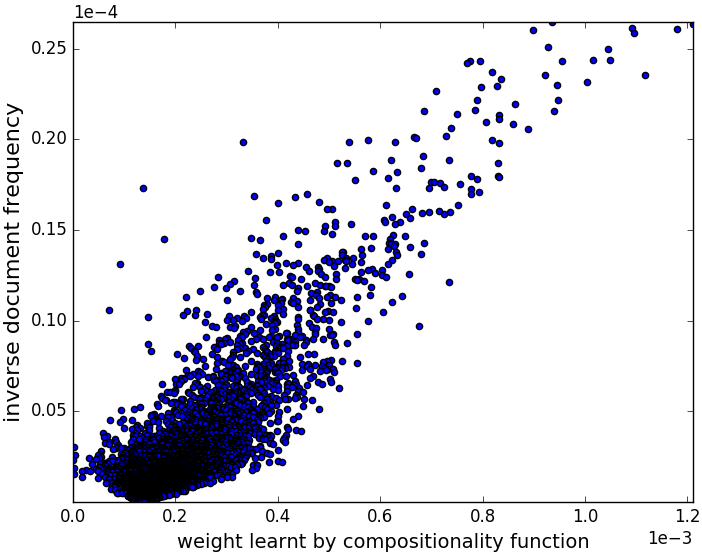
\includegraphics[height=5cm]{03-part-02/chapter-04/figs_and_tables/plot_composionality_idf_scatter_robust.png}
        \caption{\label{fig:scatter_r}Robust04}{\scriptsize{(Pearson Correlation: 0.8243)}}
    \end{subfigure}%
    ~
    \begin{subfigure}[t]{0.45\textwidth}
        \centering
        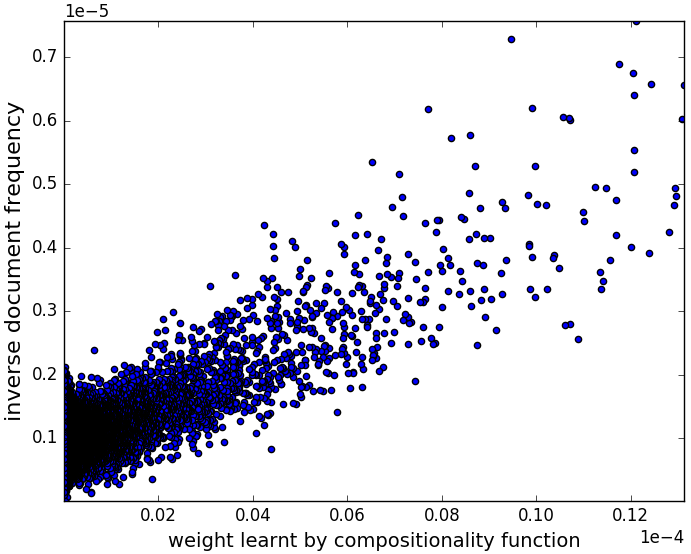
\includegraphics[height=5cm]{03-part-02/chapter-04/figs_and_tables/plot_composionality_idf_scatter_clueweb.png}
        \caption{\label{fig:scatter_c}ClueWeb}{\scriptsize{(Pearson Correlation: 0.7014)}}
    \end{subfigure}%
    \caption{\label{fig:scatter}Strong linear correlation between weight learned by the compositionality function in the \feedthree and inverse document frequency.}
\end{figure}
%
Figure~\ref{fig:scatter} illustrates the scatter plots of the learned weight for each vocabulary term and its IDF, in both collections.
This is an interesting observation as we do not provide any global corpus information to the network in training and the network is able to infer such global information by only observing individual training samples.
% This demonstrates the ability of neural networks to automatically extract meaningful features for the task.

\input{03-part-02/chapter-04/figs_and_tables/table_diff_embeddings_results.tex}
\subsubsection{How well do other alternatives for the embedding and weighting functions in the \feedthree perform?}
Considering \feedthree as the input representation, we have examined different alternatives for the embedding function $\mathcal{E}$: (1) employing pre-trained word embeddings learned from an external corpus (we used Google News), (2) employing pre-trained word embeddings learned from the target corpus (using the skip-gram model \cite{Mikolov:2013}), and (3) learning embeddings during the network training as it is explained in Section~\ref{sec:feedthree}. 
Furthermore, for the compositionality function $\odot$, we tried different alternatives: (1) uniform weighting (simple averaging which is a common approach in compositionality function), (2) using IDF as fixed weights instead of learning the weighting function $\mathcal{W}$, and (3) learning weights during the training as described in Section~\ref{sec:feedthree}.

Table~\ref{tbl_res_m3f3_em} presents the performance of all these combinations on both collections. 
We note that learning both embedding and weighting functions leads to the highest performance in both collections. These improvements are statistically significant.
%
According to the results, regardless of the weighting approach, learning embeddings during training outperforms the models with fixed pre-trained embeddings.
%
This supports the hypothesis that with the \feedthree the neural networks learn an embedding that is based on the interactions of query and documents that tends to be tuned better to the corresponding ranking task.
%
Also, regardless of the embedding method, learning weights helps models to get better performance compared to the fixed weightings, with either IDF or uniform weights. 
%
Although weight learning can significantly affect the performance, it has less impact than learning embeddings.

Note that in the models with pre-trained word embeddings, employing word embeddings trained on the target collection outperforms those trained on the external corpus in the ClueWeb collection; while this is not the case for the Robust04 collection. The reason could be related to the collection size, since the ClueWeb is approximately $100$ times larger than the Robust04.

\begin{figure}[t]
    \centering
    \begin{subfigure}[t]{0.45\textwidth}
        \centering
        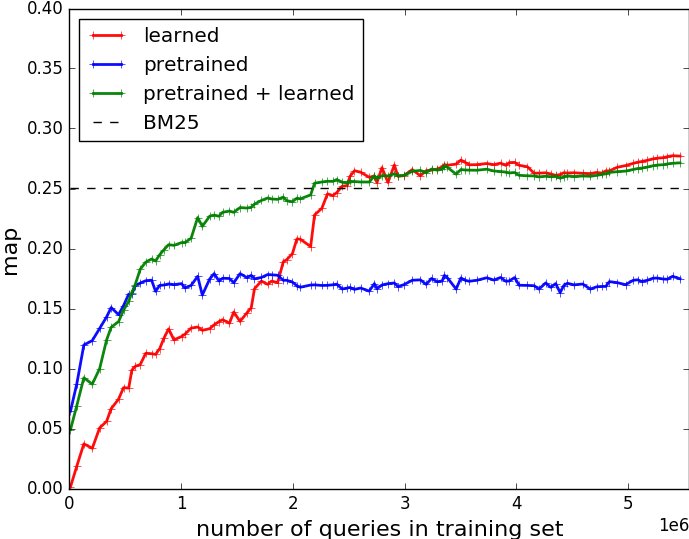
\includegraphics[height=5cm]{03-part-02/chapter-04/figs_and_tables/plot_with_pretrained_emb_robust.png}
        \caption{\label{fig:embedding_r}Robust04}
    \end{subfigure}%
    ~
    \begin{subfigure}[t]{0.45\textwidth}
        \centering
        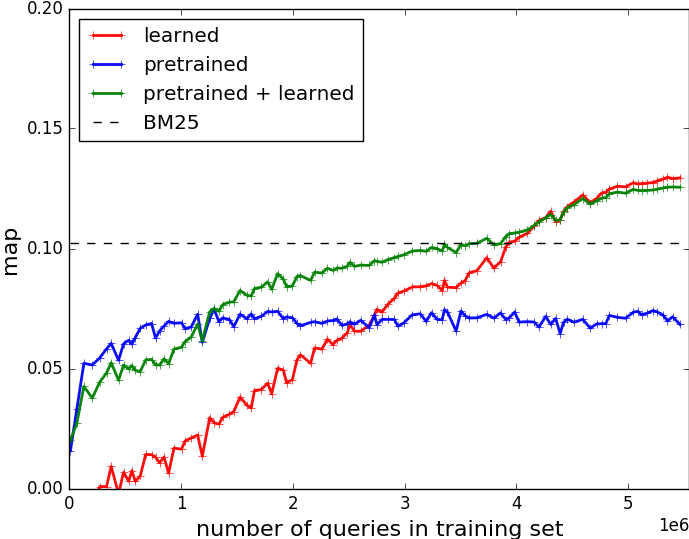
\includegraphics[height=5cm]{03-part-02/chapter-04/figs_and_tables/plot_with_pretrained_emb_clueweb.png}
        \caption{\label{fig:embedding_c}ClueWeb}
    \end{subfigure}%
    \caption{\label{fig:embedding}Performance of the \modelthree with learned embedding, pre-trained embedding, and learned embedding with pre-trained embedding as initialization, with respect to different amount of training data.}
\end{figure}

In addition to the aforementioned experiments, we have also tried initializing the embedding matrix with a pre-trained word embedding trained on the Google News corpus, instead of random initialization.
%
Figure~\ref{fig:embedding} presents the learning curve of the models. According to this figure, the model initialized by a pre-trained embedding performs better than random initialization when a limited amount of training data is available. 
%
When enough training data is fed to the network, initializing with pre-trained embedding and random values converge to the same performance.
An interesting observation here is that in both collections, these two initializations converge when the models exceed the performance of the weak supervision source, which is BM25 in our experiments. 
This suggests that the convergence occurs when accurate representations are learned by the networks, regardless of the initialization.

%In other words, after the network sees enough amount of train data to go beyond the supervision signal, it does not matter that with which initialization the model has started to train.
\input{03-part-02/chapter-04/figs_and_tables/table_svm_results.tex}
\subsubsection{Are deep neural networks a good choice for learning to rank with weak supervision?}
%
To see if there is a real benefit from using a non-linear neural network in different settings, we examined RankSVM~\citep{Joachims:2002} as a strong-performing pair-wise learning to rank method with the linear kernel that is fed with different inputs: \feedone, \feedtwo, and \feedthree. Considering that off-the-shelf RankSVM is not able to learn embedding representations during training, for \feedthree, instead of learning embeddings we use a pre-trained embedding matrix trained on Google News and fixed IDF weights. 

The results are reported in Table~\ref{tbl_svm}. As BM25 is not a linear function, RankSVM with the linear kernel is not able to completely approximate it. However, surprisingly, for both \feedone and \feedtwo, RankSVM works as well as neural networks (see Table~\ref{tbl_main}). 
%
Also, compared to the corresponding experiment in Table~\ref{tbl_res_m3f3_em}, the performance of the neural network with an external pre-trained embedding and IDF weighting is not considerably better than RankSVM. 
This shows that having non-linearity in neural networks does not help that much when we do not have representation learning as part of the model.
%
Note that all of these results are still lower than BM25, which shows that they are not good at learning from weak supervision signals for ranking. 
%

We have also examined the \modelone with a network with a single linear hidden layer, with the \feedthree, which is equivalent to a linear regression model with the ability of representation learning. 
Comparing the results of this experiment with \mone-\fthree in Table~\ref{tbl_main}, we can see that with a single-linear network we are not able to achieve a performance that is as good as a deep neural network with non-linearity.
%
This shows that the most important superiority of deep neural networks over other machine learning methods is their ability to learn an effective representation and take all the interactions between query and document(s) into consideration for approximating an effective ranking/scoring function. 
This can be achieved when we have a deep enough network with non-linear activations.

%\alexi{Mosi@: we should also include supervised learning experiments on smaller subsets of human judgments, if possible. The idea is that in these scenarios where labeled data is scarce, weak supervision is really useful. Having plots, where we use various percentages of labeled examples and observing how weak supervision is increasingly important as the number of labeled examples becomes smaller.}
\input{03-part-02/chapter-04/figs_and_tables/table_semisup_results.tex}
\subsubsection{How useful is learning with weak supervision for supervised ranking?}
%
In this set of experiments, we investigate whether employing weak supervision as a pre-training step helps to improve the performance of supervised ranking, when a small amount of training data is available. Table~\ref{tbl_semisup} shows the performance of the \modelthree with the \feedthree in three situations: (1) when it is only trained on weakly supervised data (similar to the previous experiments), (2) when it is only trained on supervised data, i.e., relevance judgments, and (3) when the parameters of the network is pre-trained using the weakly supervised data and then fine-tuned using relevance judgments.
%
In all the supervised scenarios, we performed 5-fold cross-validation over the queries of each collection and in each step, we used the TREC relevance judgments of the training set as a supervised signal. For each query with $m$ relevant documents, we also randomly sampled $m$ non-relevant documents as negative samples. Binary labels are used in the experiments: $1$ for relevant documents and $0$ for non-relevant ones.

The results in Table~\ref{tbl_semisup} suggest that pre-training the network with a weak supervision signal, significantly improves the performance of supervised ranking.
%
The reason for the poor performance of the supervised model compared to the conventional learning to rank models is that the number of parameters is much larger, hence it needs much more data for training.

In situations when little supervised data is available, it is especially helpful to use unsupervised pre-training which acts as a network pre-conditioning that puts the parameter values in the appropriate range that renders the optimization process more effective for further supervised training~\citep{Rrhan:2010}.

With this experiment, we indicate that the idea of learning from weak supervision signals for neural ranking models, which is presented in this section, not only enables us to learn neural ranking models when no supervised signal is available, but also has substantial positive effects on the supervised ranking models with limited amount of training data. 
\section{Weakly Supervised Learning for Preserving Privacy}
Deep neural networks perform better as the training dataset grows bigger and becomes more diverse and more representative~\citep{sun2017revisiting}.  In many applications, such data contains sensitive information from users, for instance medical histories of patients in a clinical trial, or search logs from users of a search engine.  
It has been shown that a trained model may inadvertently
and implicitly store some of its training data and we can retrieve some of the information about samples in the training data~\citep{Shokri:2015}, either by directly by analyzing internal model parameters or indirectly by repeatedly querying the model as a black-box to gather data and do analysis on those data~\citep{Fredrikson:2015}. 

This requires us to design and use the learning algorithms that protect the privacy of users, for instance by guaranteeing that the output model generalizes away from the specifics of any
individual user. Recently, \citet{Papernot:2017} proposed Private Aggregation of Teacher Ensembles (PATE), a generally applicable approach to providing strong privacy guarantees for training data.  PATE uses a noisy aggregation of the signal that comes from multiple models trained with disjoint datasets, to train a new model that guarantees a certain level of deferentially privacy.

Almost all deferentially private algorithms add noise to introduce ambiguity. Hence, the training signals become less perfect and employing noise-robust models can support injecting noise, yielding strong privacy guarantees, while having a limited impact on accuracy.

Search and retrieval is one of the applications that needs special attention on preserving privacy of users' data and many recent advances rely on sensitive and private data such as large-scale query logs, users’ search history, and location information~\citep{Yang:2017}. Following the previous section, we focus on the task of ranking and assessing the relevance.
Here we seek the answer to the third research question of this chapter:
\begin{resqbox}
\emph{\resq{c4.3}}
\end{resqbox}

We present the results of a set of preliminary experiments that examine the performance of one the neural ranking architectures proposed in Section~\ref{sec:weakly_supervised_neural_rankers} when it is employed in PATE, the privacy preserving framework proposed by~\citet{Papernot:2017}, where the neural ranker is supposed to learn from the signals with added noise. 
Since PATE is based on knowledge distillation framework~\cite{Hinton:2015}, we first train a neural ranker in a mimic-learning setup where a student ranker is trained on the signals from a teacher ranker that is trained using labeled data. Then we use the full privacy preserving pipeline of PATE to train our neural ranker.
%
It is noteworthy that here, we mainly concern about the performance of a neural ranker, when it is employed in the PATE's setup and will not re-discuss the differential privacy of PATE, as this side of the discussion is presented thoroughly in the original paper~\citep{Papernot:2017}.

\subsection{Mimic Learning to Rank}
\label{sec:mimic_learning_to_rank}
Using machine learning-based approaches, sharing the trained model instead of the original data has turned out to be an option for transferring knowledge~\citep{Papernot:2017,Shokri:2015,Abadi:2016}. 
The idea of \emph{mimic learning} is to use a model that is trained based on the signals from the original training data to annotate a large set of unlabeled data and use these labels as training signals for training a new model. 
It has been shown, for many tasks in computer vision and natural language processing, that we can transfer knowledge this way and the newly trained models perform as well as the model trained on the original training data~\citep{Bucilua:2006,Hinton:2015,Romero:2014,Ba:2014}.

We follow the knowledge distillation approach~\cite{Hinton:2015} for training a neural ranker, where we have a teacher network which is trained using labeled data, and a student network which is trained using the signals from the teacher network on a set of unlabeled data. We have two sets of experiments, in the first one, we train the teacher model with full supervision, i.e., on the set of queries with judgments, using 5-fold cross validation. 
In the second set of experiments, the set of queries with judgments is only used for evaluation and we train the teacher model using the weak supervision setup, i.e pseudo labels as it is explained in~\ref{sec:pseudo_labeling}. 
As the test collection, we use Robust04 which is introduced in Section~\ref{sec:collections}. In all experiments, we use a separate set of $3$ million queries from the AOL query log, preprocessed as it is explained in Section~\ref{sec:query_set}.

In all experiments, as the neural rankers we use \modeltwo, which has been described in Section~\ref{sec:modeltwo}, with \Feedthree as the input representation, which has been explained in Section~\ref{sec:feedthree}.  The configuration of teacher and student networks is presented in Table~\ref{tbl:cfg}.
\begin{table}[t]
\centering
\caption{Teacher and student neural networks configurations.}
\begin{tabular}{lcc} 
\toprule
\bf Parameter & \bf Teacher & \bf Student  \\
\midrule
 Number of hidden layers & 3 & 3  \\
 Size of hidden layers & 512 & 128 \\
 Initial learning rate & 1E-3 & 1E-3 \\
 Dropout & 0.2 & 0.1 \\
 Embedding size & 500 & 300 \\
 Batch size & 512 & 512  \\
\bottomrule
\end{tabular}
\label{tbl:cfg}
\end{table}

\begin{table}[t]
\centering
\caption{\label{tbl_res1}Performance of teacher and student models with different training strategies.}
\vspace{5pt}
\begin{adjustbox}{max width=\textwidth}
\begin{tabular}{l l c c c}
\toprule
\bf Training strategy & \bf model & \textbf{MAP} & \textbf{P@20} & \textbf{nDCG@20} 
\\ \midrule
\multirow{2}{*}{{Full supervision}} & {Teacher} 
& 0.1814 & 0.2888 & 0.3419 
\\
& {Student} 
& 0.2256 & 0.3111 & 0.3891 
\\ \midrule
\multirow{2}{*}{{Weak supervision}} & {Teacher} 
& 0.2716 & 0.3664 & 0.4109 
\\ 
& {Student} 
& 0.2701 & 0.3562 & 0.4145 
\\ \bottomrule
\end{tabular}
\end{adjustbox}
\end{table}

Results obtained from these experiments are summarized in Table~\ref{tbl_res1}. As the results suggest, using weak supervision to train the teacher model, the student model performs as good as the teacher model. In case of training the teacher with full supervision (labeled data from Robust04), as the original training data is small, the performance of the teacher model is rather low, which is mostly due to the fact that the big teacher model overfits on the train data and is not able to generalize well. 
However, due to the regularization effect of knowledge distillation process, the student model, which is trained on the predictions by the teacher model significantly outperforms the teacher model~\citep{Hinton:2015,Romero:2014}.

\subsection{Privacy Preserving Neural Ranker}
In Section~\ref{sec:mimic_learning_to_rank}, we examined the idea of mimic learning to train a neural ranker regardless of the privacy concerns.
It has been shown that there is a risk of privacy problems, both where the adversary is just able to query the model, and where the model parameters are exposed to the adversaries inspection.
For instance, \citet{Fredrikson:2015} show that only by observing the prediction of the machine learning models they can approximately reconstruct part of the training data (model-inversion attack). \citet{Shokri:2016} also demonstrate that it is possible to infer whether a specific training point is included in the model's training data by observing only the predictions of the model (membership inference attack).

In this section, we adapt the Private Aggregation of Teacher Ensembles (PATE)~\citep{Papernot:2017} to train a privacy preserving neural ranking model.  PATE is based on student-teacher framework\cite{Hinton:2015}, where there are multiple teacher models trained on disjoint subsets of the data and a student model that learns to predict an output that is chosen by noisy voting among all of the teachers. The student model cannot directly access an individual teacher or the underlying data or parameters. They show that PATE improves privacy/utility trade-offs by achieving high accuracy, while guaranteeing a certain level of differential privacy.

\begin{figure}[t]
    \centering
    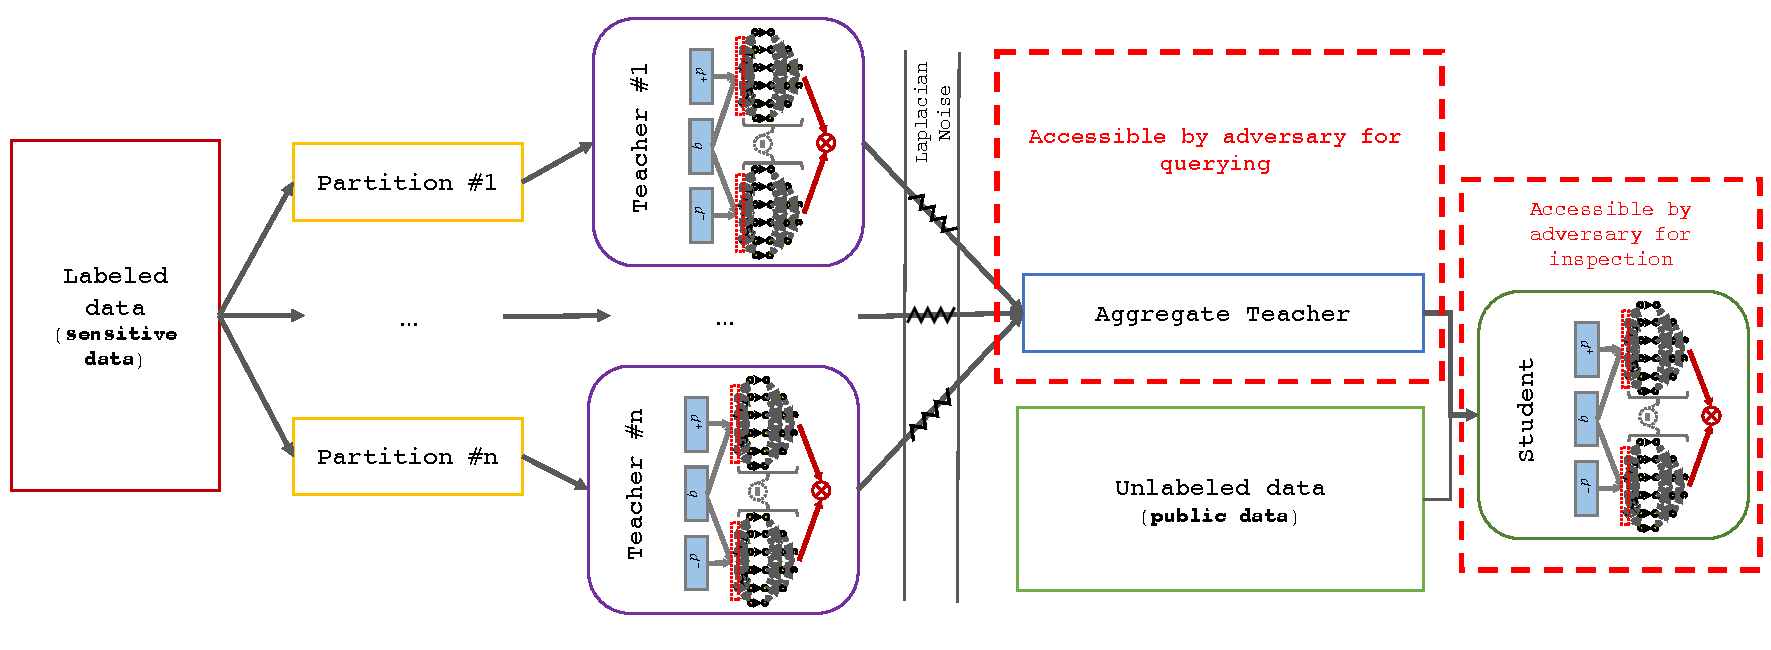
\includegraphics[height=5.5cm]{03-part-02/chapter-04/figs_and_tables/fig_privacy_preserving_ranker_model.pdf}%
    \caption{\label{fig:pp_model} Privacy preserving annotator/model sharing, proposed by~\citet{Papernot:2017}.}
\end{figure}

The general schema of the PATE is illustrated in Figure~\ref{fig:pp_model}. First, the sensitive training data is divided into $n$ partitions. Then, on each partition, an independent neural network model is trained as a teacher.  Once all the teachers are trained, an aggregation step is done using majority voting to generate a single global prediction.  
Laplacian noise is injected into the output of the prediction of each teacher before aggregation. The introduction of this noise is what protects privacy because it obfuscates the vulnerable cases, where teachers disagree. 

The aggregated teacher can be considered as a deferentially private API to which we can submit the input and it then returns the privacy preserving label. There are some circumstances where due to efficiency reasons the model is needed to be deployed to the user device~\cite{Abadi:2016}. To be able to generate a shareable model where the privacy of the training data is preserved, \citet{Papernot:2017} train an additional model called the student model. The student model has access to unlabeled public data during training. The unlabeled public data is annotated using the aggregated teacher to transfer knowledge from teachers to student model in a privacy preserving fashion. 
This way, if the adversary tries to recover the training data by inspecting the parameters of the student model, in the worst case, the public training instances with privacy preserving labels from the aggregated teacher are going to be revealed.  The privacy guarantee of this approach is formally proved using differential privacy framework.

As there is no publicly available large scaled data that we can use in our experiments as the initial sensitive labeled data, we use pseudo labels as it is explained in~\ref{sec:pseudo_labeling}\footnote{Partitioning the fully supervised training data in our problem leads to very small training sets which are not big enough to train teacher networks.}. 
In our experiments, we split the training data into three partitions, each contains one million queries annotated by the BM25 method. We train three identical teacher models. Then, we use the aggregated noisy predictions from these teachers to train the student network using the knowledge distillation approach. Configurations of teacher and student networks are similar to the previous experiments, as they are presented in Table~\ref{tbl:cfg}.

We evaluate the performance in two situations: In the first one, the privacy parameter, which determines the amount of noise, is set to zero, and in the second one, the noise parameter is set to $0.05$, which guarantees a low privacy risk~\citep{Papernot:2017}.
%
We report the average performance of the teachers before noise, the performance of noisy and non-noisy aggregated teacher, and the performance of the student networks in two situations.  The results of these experiments are reported in Table~\ref{tbl_res2}.

\begin{table}[t]
\centering
\caption{\label{tbl_res2}Performance of the teachers (average) and student models with noisy and non-noisy aggregation.}
\vspace{5pt}
\begin{adjustbox}{max width=\textwidth}
\begin{tabular}{l c c c}
\toprule
 \bf Model & \textbf{MAP} & \textbf{P@20} & \textbf{nDCG@20} 
\\ \midrule
{Teachers (avg)} 
& 0.2566 & 0.3300 & 0.3836
\\ \midrule
{Non-noisy aggregated teacher} 
& 0.2380 & 0.3055 & 0.3702 
\\
{Student \small{(non-noisy aggregation)}} 
& 0.2337 & 0.3192 & 0.3717
\\ \midrule 
{Noisy aggregated teacher} 
& 0.2110 & 0.2868 & 0.3407 
\\
{Student \small{(noisy aggregation)}} 
& 0.2255 & 0.2984 & 0.3559 
\\ \bottomrule
\end{tabular}
\end{adjustbox}
\end{table}

Results in Table~\ref{tbl_res2} suggest that using the noisy aggregation of multiple teachers as the supervision signal, we can train a neural ranker with an acceptable performance.
%
Compared to the single teacher setup in Section~\ref{sec:mimic_learning_to_rank}, the performance of the student network is not as good as the average performance of teachers. Although the student network performs better than the teacher in the noisy aggregation setup. This is more or less the case for a student together with a non-noisy aggregated teacher.
% 
We believe drops in the performance on the student networks compared to the results in Section~\ref{sec:mimic_learning_to_rank} are not just due to partitioning, noise, and aggregation. This is also the effect of the change in the amount of training data for the teachers in our experiments. We speculate that in the case of having enough training data in each partition for each teacher, their prediction will be more determined and we will have less disagreement in the aggregation phase and consequently, we will get better signals for training the student model.



\section{Related Work}
In this section, we briefly review the neural ranking models in terms of their general architectures and discuss how the neural models proposed in this chapter are related to the previous works.

Recently, several attempts have been made to study deep neural networks in IR applications, which can be generally partitioned into two categories~\citep{guo2019deep, Onal:2016, Zhang:2016}. 
The first category includes approaches that use the results of trained (deep) neural networks in order to improve the performance in IR applications. Among these, distributed word representations or embeddings~\citep{Mikolov:2013,Pennington:2014} have attracted a lot of attention. Word embedding vectors have been applied to term re-weighting in IR models~\citep{Zheng:2015}, query expansion~\citep{Diaz:2016,Zamani:2016a}, query classification~\citep{Liu:2015,Zamani:2016b},  etc. 
The main shortcoming of most of the approaches in this category is that the objective of the trained neural network differs from the objective of these tasks.  For instance, the word embedding vectors proposed in~\citep{Mikolov:2013,Pennington:2014} are trained based on term proximity in a large corpus, which is different from the objective in most IR tasks. \citet{Zamani:2017} recently proposed relevance-based word embedding models for learning word representations based on the objectives that matter for IR applications.

The second category, which the models proposed in this chapter belong to, consists of the approaches that design and train a (deep) neural network for a specific task, e.g., question answering~\citep{Cohen:2016,Yang:2016}, click models~\citep{Borisov:2016}.
A number of the approaches in this category have been proposed for ranking documents in response to a given query.
These approaches can be generally divided into two groups: \emph{late combination models} and \emph{early combination models} (or representation-focused and interaction-focused models according to~\citep{Guo:2016}). 
The late combination models, following the idea of Siamese networks~\citep{Bromley:1993}, independently learn a representation for each query and candidate document and then calculate the similarity between the two estimated representations via a similarity function. For example, \citet{Huang:2013} proposed DSSM, which is a feed forward neural network with a word hashing phase as the first layer to predict the click probability given a query string and a document title. 
The DSSM model was further improved by incorporating convolutional neural networks~\citep{Shen:2014}.

On the other hand, the early combination models are designed based on the interactions between the query and the candidate document as the input of network. 
For instance, DeepMatch~\citep{Lu:2013} maps each text to a sequence of terms and trains a feed-forward network for computing the matching score. 
The deep relevance matching model for ad-hoc retrieval~\citep{Guo:2016} is another example of an early combination model that feeds a neural network with the  histogram-based features representing interactions between the query and document. 
Early combining enables the model to have an opportunity to capture various interactions between query and document(s), while with late combination approach, the model has only the chance of isolated observation of input elements. Recently, Mitra et al.~\citep{Mitra:2016} proposed to simultaneously learn local and distributional representations, which are early and late combination models respectively,  to capture both exact term matching and semantic term matching.

Until now, all the proposed neural models for ranking are trained on either explicit relevance judgements or clickthrough logs. However, a massive amount of such training data is not always available. 

In this chapter, we propose to train neural ranking models using weak supervision, which is the most natural way to reuse the existing supervised learning models where the imperfect labels are treated as the ground truth.
The basic assumption is that we can cheaply obtain labels (that are of lower quality than human-provided labels) by expressing the prior knowledge we have about the task at hand by specifying a set of heuristics, adapting existing ground truth data for a different but related task (this is often referred to distant supervision\footnote{We do not distinguish between weak and distant supervision as the difference is subtle and both terms are often used interchangeably in the literature.}), extracting supervision signal from external knowledge-bases or ontologies, crowd-sourcing partial annotations that are cheaper to get, etc.
%
Weak supervision is a natural way to benefit from unsupervised data and it has been applied in NLP for various tasks including relation extraction~\citep{Bing:2015,Han:2016}, knowledge-base completion~\citep{Hoffmann:2011}, sentiment analysis~\citep{Severyn:2015:SemEval}, etc.  
There are also similar attempts in IR for automatically constructing test collections~\citep{Asadi:2011} and learning to rank using labeled features, i.e., features that an expert believes they are correlated with relevance~\citep{Diaz:2016:ictir}.
In this chapter, we make use of traditional IR models as the weak supervision signal to generate a large amount of training data and train effective neural ranking models that outperform the baseline methods by a significant margin.


%%%%%%%%%%%%%%%%%%%%%%%%%%%%%%%%%%%%%%%%%%%%%%%%%%%%%%%%%%%%%%%%%%%%%%%%%%%%%%%%%%%%%%%%%%%%%%%%%%%%%%%%%%%%%%%%%%%%%%%%%%%%%%%%%%%%%%%%%%%%%%%%%%%%%%%%%%%%%%%%%%%%%%%%%%%%%%%%%%%%%%%%%%%%%%%%%%%%%%%%%%%%%%%%%%%%%%%%%%%%%%%%%%%%%%%%%%%%%%%%%%%%%%%%%%%%%%%%%%%%%%%%%%%%%%%%%%%%%%%%%%%%%%%%%%%%%%%%%%%%%%%%%%%%%%%%%%%%%%%%%%%%%%%%%%



To circumvent the lack of human-labeled training examples, unsupervised learning methods aim to model the underlying data distribution, thus learning powerful feature representations of the input data, which can be helpful for building more accurate discriminative models especially when little or even no supervised data is available. A large group of unsupervised neural models seeks to exploit the implicit internal structure of the input data, which in turn requires customized formulation of the training objective (loss function), targeted network architectures and often non-trivial training setups. 


For example in NLP, various methods for learning distributed word representations, e.g., word2vec~\citep{Mikolov:2013}, GloVe~\citep{Pennington:2014}, and sentence representations, e.g., paragraph vectors~\citep{Le:2014} and skip-thought~\citep{Kiros:2015} have been shown very useful to pre-train word embeddings that are then used for other tasks such as sentence classification, sentiment analysis, etc. Other generative approaches such as language modeling in NLP, and, more recently, various flavors of auto-encoders~\citep{Baldi:2012} and generative adversarial networks~\citep{Goodfellow:2014} in computer vision have shown a promise in building more accurate models.






A lot of research has been done on the general problem of preserving the privacy of sensitive data in IR applications, where the question is how should we design effective IR systems without damaging users' privacy?  One of the solutions so far is to anonymize the data and try to hide the identity of users~\citep{Carpineto:2013, Zhang:2016}.  As an example, \citet{Zhang:2016} use a differential privacy approach for query log anonymization. However, there is no guarantee that the anonymized data will be as effective as the original data.

Modeling privacy in machine learning is a challenging problem and there has been much research in this area. Preserving the privacy of deep learning models is even more challenging, as there are more parameters to be safeguarded~\citep{Phan:2016}. 
Some work has studied the vulnerability of deep neural network as a service, where the interaction with the model is only via an input-output black box~\citep{Tramer:2016, Fredrikson:2015, Shokri:2016}.
Others have proposed approaches to protect privacy against an adversary with a full knowledge of the training mechanism and access to the model's parameters. For instance, \citet{Abadi:2016} propose a privacy preserving stochastic gradient descent algorithm offering a trade-off between utility and privacy. More recently, \citet{Papernot:2017} propose a semi-supervised method for transferring the knowledge for deep learning from private training data. They propose a setup for learning privacy-preserving student models by transferring knowledge from an ensemble of teachers trained on disjoint subsets of the data for which privacy guarantees are provided.


\section{Conclusion}
In this chapter, we focused on addressing \textbf{\resqname{c4}}. 
We proposed to use unsupervised methods in order to programmatically generate large amounts of training data, as weakly annotated data, to train effective neural ranking models. We focus on the task of assessing the relevance, i.e., ranking documents given a query that suffers from a large-scale publicly available training set. We examined various neural ranking models with different ranking architectures and objectives, and different input representations. 

To investigate \textbf{\resqname{c4.1}}, We used over six million queries to train our models and evaluated them on Robust04 and ClueWeb 09-Category B collections, in an ad-hoc retrieval setting.  The experiments showed that our best performing model significantly outperforms the BM25 model (our weak supervision signal) by over $13\%$ and $35\%$ MAP improvements in the Robust04 and ClueWeb collections, respectively. 
We also demonstrated that in the case of having a small amount of training data, we can improve the performance of supervised learning by pre-training the network on weakly supervised data.

To address \textbf{\resqname{c4.2}}, we showed that based on our results, there are three key ingredients in neural ranking models that lead to good performance with weak supervision:
%
The first is the proper input representation. Providing the network with raw data and letting the network to learn the features that matter, gives the network a chance of learning how to ignore imperfection in the training data.
%
The second ingredient is to target the right goal and define a proper objective function. In the case of having weakly annotated training data, by targeting some explicit labels from the data, we may end up with a model that learned to express the data very well, but is incapable of going beyond it. 
This is especially the case with deep neural networks where there are many parameters and it is easy to learn a model that overfits the data.
%
The third ingredient is providing the network with a considerable amount of diverse training examples. 
As an example, during the experiments we noticed that using the \feedthree, the network needs a lot of examples to learn embeddings that are more effective for retrieval compared to pre-trained embeddings. 
Thanks to weak supervision, we can generate as much training data as we need with almost no cost.

To address \textbf{\resqname{c4.3}}, we also study how learning from weak signals can benefit preserving privacy where some noise is intentionally added to the training signal to preserve privacy. We employed Private Aggregation of Teacher Ensembles (PATE)~\citep{Papernot:2017}  to train a privacy-preserving neural ranking model, in which we train several neural rankers on disjoint subsets of the training data and use the noisy aggregated signals from these models on an unlabeled set to train a neural ranker that in a setup that guarantees a certain level of differential privacy.
These experiments lay the groundwork for the idea of sharing a privacy-preserving model instead of sensitive data in IR applications. This suggests researchers from industry share the knowledge learned from actual users' data with the academic community that leads to a better collaboration of all researchers in the field. 

% connection to chapter 5
In this chapter, we mainly focused on the ranking task and explored architectural ideas that can implicitly help to have neural networks that are less sensitive to the label noise.  
In the next chapter, we propose more systematic approaches that are tasks and architecture independent and can learn to estimate the quality of the labels and explicitly control the learning process with respect to the estimated qualities.
% \chapter{\titleof{c5}}
\blankfootnote{This chapter is based on \citep{dehghani:2018:ICLR,Dehghani:2017:nips_metalearn,Dehghani:2017avoiding}.}

\label{chap:5}
%
\begin{quote}
Training labels are expensive to obtain and may be of varying quality, as some may be from trusted expert labelers, while others might be from heuristics or other sources of weak supervision. This creates a fundamental quality-versus-quantity trade-off in the learning process.  Do we learn from the small amount of high-quality data or the potentially large amount of weakly-labeled data? We argue that if the learner could somehow know and take the label-quality into account, we could get the best of both worlds.
\end{quote}
%
\section{Introduction}
The success of deep neural networks to date depends strongly on the availability of labeled data. The more neural networks become deep and complex, the more it is crucial for them to be trained on massive amounts of training data. However, in many applications, labeled data is costly to obtain and task-specific training data is now a critical bottleneck. 

Usually, it is much easier to obtain small quantities of high-quality labeled data and large quantities of unlabeled data. The problem of how to best integrate these two different sources of information during training is an active pursuit in the field of semi-supervised learning~\citep{chap:semi06}.
However, for a large class of tasks it is also easy to define one or more so-called ``weak annotators'', additional (albeit noisy) sources of \emph{weak supervision} based on heuristics or ``weaker'', biased classifiers trained on e.g.\ non-expert crowd-sourced data or data from different domains that are related. 
While easy and cheap to generate, it is not immediately clear if and how these additional weakly-labeled data can be used to train a stronger classifier for the task we care about.

All labels are equal, but some labels are more equal than others~\footnote{Inspired by George Orwell quote, Animal Farm, 1945}. This holds generally since in almost all practical applications, machine learning systems have to deal with data \emph{samples of variable quality}. For example, in a large dataset of images, only a small fraction of samples may be labeled by experts and the rest may be crowd-sourced using e.g.\ Amazon Mechanical Turk~\citep{Veit:2017}. In addition, in some applications, labels are intentionally perturbed due to privacy issues~\citep{wainwright2012privacy,Papernot:2016, dehghani:2017:neuir}. 

Formally speaking, in our setup, we assume that we are given a large set of unlabeled data samples, a heuristic labeling function called the \emph{\wa}, and a small set of high-quality samples labeled by experts, called the \emph{strong dataset}, consisting of tuples of training samples $x_i$ and their true labels $y_i$, i.e., $\mathcal{D}_s=\{(x_i,y_i)\}$. We consider the latter to be observations from the true target function that we are trying to learn. 
We use the \wa to generate labels for the unlabeled samples. Generated labels are noisy due to the limited accuracy of the \wa. This gives us the \emph{weak dataset} consisting of tuples of training samples $x_i$ and their weak labels $\tilde{y}_i$, i.e., $\mathcal{D}_w=\{(x_i, \tilde{y}_i)\}$.  Note that we can generate a large amount of weak training data $\mathcal{D}_w$ at almost no cost using the \wa. In contrast, we have only a limited amount of observations from the true function, i.e., $|\mathcal{D}_s| \ll |\mathcal{D}_w|$. 

The simplest approach in this setup is to expand the strong training set, $\mathcal{D}_s$, by including the weakly-supervised samples, $\mathcal{D}_w$, which is, in fact, considering all samples are equally important. Alternatively, one may pretrain on the weak data and then fine-tune on observations from the true function or distribution (which we call strong data). Indeed, it has been shown that a small amount of expert-labeled data can be augmented in such a way by a large set of raw data, with labels coming from a heuristic function, to train a more accurate ranking model~\citep{Dehghani:2017:SIGIR, Severyn:2015:SIGIR}.
The downside is that such approaches are oblivious to the amount or source of noise in the labels. Simply speaking, they do not consider the cause of noise in the labels and only focus on the effect. 

In this chapter, we focus on this issue and try to address the following research question:
\resq{c5}

We argue that treating weakly-labeled samples uniformly (i.e.\ each weak sample contributes equally to the final classifier) ignores potentially valuable information of the label quality. 

Instead, we propose two different approaches that they directly model the inaccuracies introduced by the \wa, which can then be used to modulate the training process based on the fidelity (or quality) of each weak sample. 
% In other words, we control the extent to which we make use of this additional source of weak supervision: more for confidently-labeled weak samples close to the true observed data, and less for uncertain samples further away from the observed data. 


\subsection{Detailed Research Questions}
We break down our main research question in this chapter into two concrete research questions:
\begin{resqbox}
\begin{enumerate}
\item[\textbf{\resqname{c5.1}}] \emph{\resqcontent{c5.1}}
\item[\textbf{\resqname{c5.2}}] \emph{\resqcontent{c5.2}}
\end{enumerate}
\end{resqbox}
In the following sections, we will address these research questions, and support our ideas with experiments and analyses on different tasks.

\section{Learning to Learn from Weak Supervision, by Full Supervision}
\label{sec:meta_learning}
Using weak or noisy supervision is a straightforward approach to increase the size of the training data. This is usually done by pre-training the network on a large set of weakly labeled data and fine-tuning it with strong labels~\cite{Dehghani:2017:SIGIR,Severyn:2015:SIGIR}. 
However, these two independent stages do not leverage the full capacity of information from the small set of strong labels.  In particular, in the pre-training stage, we have to learn from labels of variable quality without any control over how these labels contribute to the learning process.

In this section, we address the first research question of this chapter:
\resq{c5.1}

We introduce a semi-supervised method that leverages a small amount of data with strong labels to improve the learning from a large amount of data with weak labels. This model, in fact, offers learning from \emph{Controlled Weak Supervision} and we refer to it by \emph{\cws} in the rest of this chapter.
%
\cws has three main components:
A \wa, which can be a heuristic model, a weak or biased classifier, or even a human via crowd-sourcing and it is employed to annotate a massive amount of unlabeled data, a \tnet, which uses a large set of weakly annotated instances by the \wa to learn the main task, and a \cnet, which is trained on a small set with strong labels to estimate confidence scores for instances annotated by the \wa. 

The confidence scores estimated by the \cnet define the magnitude of the weight updates applied to the \tnet during training. This way, the \cnet helps the \tnet to avoid the mistakes of her teacher, i.e., \wa, by down-weighting the weight updates from weak labels that do not look reliable according to \cnet.
%
\cws, in fact, employs teacher-student paradigm in which, the \tnet (student) and the \cnet (teacher) are trained jointly in a multi-task fashion and they share parameters of the representation learning layer to share their understanding of the data.

From a meta-learning perspective~\citep{Andrychowicz:2016,Finn2017:ICML,Ravi:2016}, the goal of the \cnet, as the meta-learner, trained jointly with the \tnet, as the learner, is to calibrate the learning rate of the \tnet for each instance in the batch. I.e., the weights $\pmb{w}$ of the \tnet $f_w$ at step $t+1$ are updated as follows:
\begin{equation}
\pmb{w}_{t+1} = \pmb{w}_t - \frac{\eta_t}{b}\sum_{i=1}^b c_{\theta}(x_i, \tilde{y}_i)  \nabla \mathcal{L}(f_{\pmb{w_t}}(x_i), \tilde{y_i})
%+ \nabla \mathcal{R}(\pmb{w_t})
\end{equation}
where $\eta_t$ is the global learning rate, $\mathcal{L}(\cdot)$ is the loss of predicting $\hat{y}=f_w(x_i)$ for an input $x_i$ when the label is $\tilde{y}$; $c_\theta(\cdot)$ is a scoring function learned by the \cnet taking input instance $x_i$ and its noisy label $\tilde{y}_i$. Thus, we can effectively control the contribution to the parameter updates for the \tnet from weakly labeled instances based on how reliable their labels are according to the \cnet (learned on a small supervised data).

Our setup requires running a \wa to label a large amount of unlabeled data, which is done at pre-processing time. For a large class of tasks, it is possible to use a simple heuristic, or implicit human feedback to generate weak labels. This set is then used to train the \tnet.  
In contrast, a small expert-labeled set is used to train the \cnet, which estimates how good the weak annotations are, i.e., controls the effect of weak labels on updating the parameters of the \tnet.

\cws allows learning different types of neural architectures and various tasks, where a meaningful \wa is available. 
Later in this chapter 

we study the performance of \cws by focusing on two applications: sentiment classification and document ranking. 

\subsection{Learning from Controlled Weak Supervision}
\label{sec:method}
In the following, we describe our recipe for semi-supervised learning of neural networks, in a scenario where along with a small human-labeled training set a large set of weakly labeled instances is leveraged.

% \subsection{General Architecture}
% \label{sec:generalarchitecture}
\begin{figure}[!t]%
    \makebox[\textwidth][c]{
    \centering
    \begin{subfigure}[t]{0.5\textwidth}
        \centering
        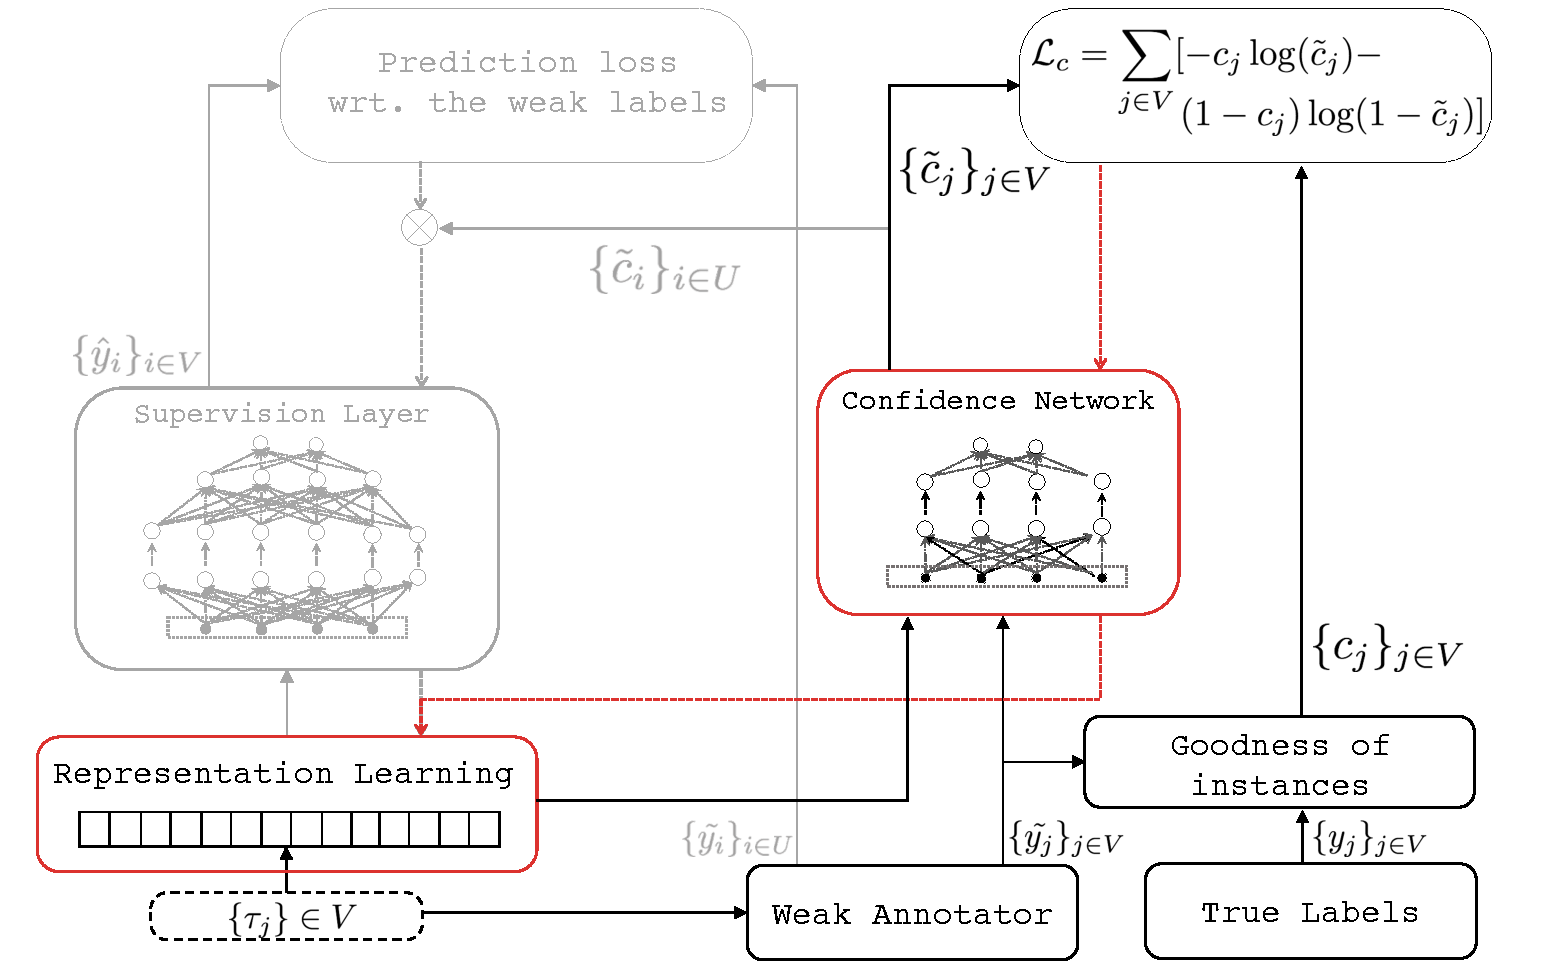
\includegraphics[width=\textwidth]{03-part-02/chapter-05/figs_and_tables/fig_cws_train_v.pdf}
        \caption{\label{fig:train_u}\footnotesize{Full Supervision Mode: Training on batches with strong labels.}}
    \end{subfigure}%
    ~
    \begin{subfigure}[t]{0.5\textwidth}
        \centering
        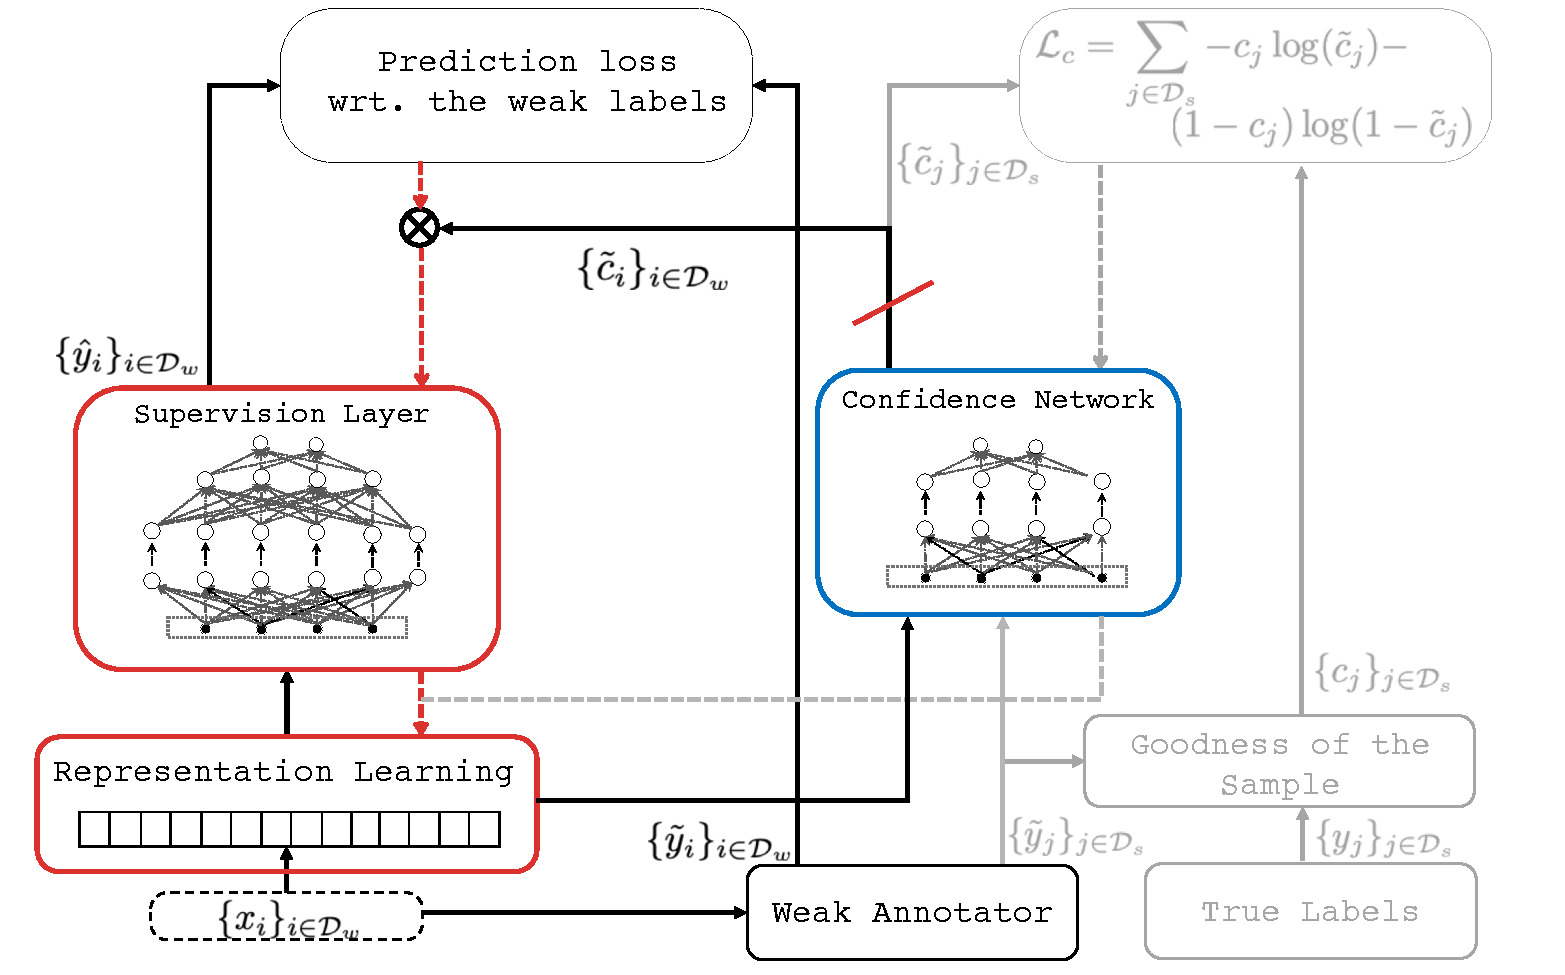
\includegraphics[width=\textwidth]{03-part-02/chapter-05/figs_and_tables/fig_cws_train_u.pdf}
        \caption{\label{fig:train_v}\footnotesize{Weak Supervision Mode: Training on batches with weak labels.}}
    \end{subfigure}%
    }
    \caption{Learning from controlled weak supervision: Our proposed multi-task network for learning a target task in a semi-supervised fashion, using a large amount of weakly labeled data and a small amount of data with strong labels.
    %
    Faded parts of the network are disabled during the training in the corresponding mode. Red-dotted arrows show gradient propagation. Parameters of the parts of the network in red frames get updated in the backward pass, while parameters of the network in blue frames are fixed during the training. (Best viewed in color.)}
    \label{fig:model_cws}
\end{figure}

In our proposed model we train a multi-task neural network that jointly learns the confidence score of weakly labeled instances and the main task using controlled supervised signals.
%
The high-level representation of the model is shown in Figure~\ref{fig:model_cws}: it comprises a \wa and two neural networks: the \cnet and the \tnet. 

The goal of the \wa is to \emph{provide weak labels} $\tilde{y}_i$ for all the instances $x_i \in U \cup V$. We have this assumption that $\tilde{y}_i$ provided by the \wa are imperfect estimates of strong labels $y_i$, where $y_i$ are available for set $\mathcal{D}_s$, but not for set $\mathcal{D}_w$.

The goal of the \cnet is to \emph{estimate the confidence score} $\tilde{c}_j$ of training instances. It is learned on examples from the training set $\mathcal{D}_s$, i.e a set of input $x_j$ and its strong label $y_j$ as well its weak label,  $\tilde{y}_j$,  that is annotated by the \wa.
The score $\tilde{c}_j$ is then used to control the effect of weakly labeled instances on updating the parameters of the \tnet in the backward pass of backpropagation.

The \tnet is in charge of \emph{handling the main task} we want to learn, or in other words, approximating the underlying function that predicts the correct labels. 
Given the data instance, $x_i$ and its weak label $\tilde{y}_i$ from the training set $\mathcal{D}_w$, the \tnet aims to predict the label $\hat{y}_i$. 
The \tnet parameter updates are based on noisy labels assigned by the \wa, but the magnitude of the gradient update is based on the output of the \cnet. 

Both networks are trained in a multi-task fashion alternating between the \emph{full supervision} and the \emph{weak supervision} mode.  
In the \emph{full supervision} mode, the parameters of the \cnet get updated using instances from training set $\mathcal{D}_s$.  
As depicted in Figure~\ref{fig:train_v}, each training instance is passed through the representation layer mapping inputs to vectors. These vectors are concatenated with their corresponding weak labels $\tilde{y}_j$ generated by the \wa.
The \cnet, which is a fully connected feedforward network with sigmoid as the output layer, estimates $\tilde{c}_j$ that is the probability of taking data instance $j$ into account for training the \tnet.

In the \emph{weak supervision} mode, the parameters of the \tnet are updated using the training set $\mathcal{D}_w$.
As shown in Figure~\ref{fig:train_u}, each training instance is passed through the same representation learning layer and is then processed by the supervision layer which is a part of the \tnet predicting the label for the main task. 
%
We also pass the learned representation of each training instance along with its corresponding label generated by the \wa to the \cnet to estimate the \emph{confidence score} of the training instance, i.e., $\tilde{c}_i$. 
The confidence score is computed for each instance from the training set $\mathcal{D}_w$. These confidence scores are used to weight the gradient updating \tnet parameters or in other words the step size during back-propagation. 

It is noteworthy that the representation layer is shared between both networks, so besides the regularization effect of layer sharing which leads to better generalization, sharing this layer lays the ground for the \cnet to benefit from the largeness of the set $\mathcal{D}_w$ and the \tnet to utilize the quality of set $\mathcal{D}_s$. 

\subsection{Training the Learner and the Meta-Learner}
\label{sec:modeltraining}
Here, we explain how we train \cws in which we jointly update the parameters of \tnet, the learner and the \cnet, the meta-learner. 
Our optimization objective is composed of two terms: (1) the \cnet loss $\mathcal{L}_c$, which captures the quality of the output from the \cnet and (2) the \tnet loss $\mathcal{L}_t$, which expresses the quality for the main task. 

Both networks are trained by alternating between the \emph{weak supervision} and the \emph{full supervision} mode.
%
In the \emph{full supervision} mode, the parameters of the \cnet are updated using training instance drawn from training set $\mathcal{D}_s$. We use cross-entropy loss function for the \cnet to capture the difference between the predicted confidence score of instance $j$, i.e., $\tilde{c}_j$ and the target score $c_j$:
\begin{equation}
% \nonumber
\mathcal{L}_c = \sum_{j\in V} -  c_j \log(\tilde{c}_j) - (1-c_j) \log(1-\tilde{c}_j),
\end{equation}
%given that $c_j$ is not a probability I'm wondering if we can call this loss a cross-entropy --- it only makes sense if $c_j$ is a probability of binary event. Possibly, it's common to use in IR, but i've never seen it used like this on real-valued scores.} 
The target score $c_j$ indicates how similar the strong and the weak labels are, and it is calculated with respect to the main task. 

In the \emph{weak supervision} mode, the parameters of the \tnet are updated using training instances from $\mathcal{D}_w$. We use a weighted loss function, $\mathcal{L}_t$, to capture the difference between the predicted label $\hat{y}_i$ by the \tnet and target label $\tilde{y}_i$:
\begin{equation}
% \nonumber
\mathcal{L}_t = \sum_{i\in U} \tilde{c}_i \mathcal{L}_i,
\end{equation}
where $\mathcal{L}_i$ is the task-specific loss on training instance $i$ and $\tilde{c}_i$ is the confidence score of the weakly annotated instance $i$, estimated by the \cnet.
Note that $\tilde{c}_i$ is treated as a constant during the weak supervision mode and there is no gradient propagation to the \cnet in the backward pass (as depicted in Figure~\ref{fig:train_u}). 

We minimize two loss functions jointly by randomly alternating between full and weak supervision modes (for example, using a 1:10 ratio).
During training and based on the chosen supervision mode, we sample a batch of training instances from $\mathcal{D}_s$ with replacement or from $\mathcal{D}_w$ without replacement (since $\mathcal{D}_w$ can be very large). Since in our setups usually $|\mathcal{D}_w| >> \mathcal{D}_s|$, the training process oversamples the instance from $\mathcal{D}_s$. 

The key point here is that the ``main task'' and ``confidence scoring'' task are always defined to be close tasks and sharing representation will benefit the confidence network as an implicit data augmentation to compensate the small amount of data with strong labels.
Besides, we noticed that updating the representation layer with respect to the loss of the other network acts as a regularization for each of these networks and helps generalization for both target and confidence network since we try to capture all tasks (which are related tasks) and less chance for overfitting.

% We also investigated other possible setups or training scenarios. For instance, we tried updating the parameters of the supervision layer of the \tnet using also data with strong labels. Or instead of using alternating sampling, we tried training the \tnet using controlled weak supervision signals after the \cnet is fully trained.
% As shown in the experiments the architecture and training strategy described above provide the best performance.
\newcommand{\tfunc}{T} %function name for the teacher
\section{\fwlfull}
\label{sec:fidelity_weighted_learning}

In this section, we address the second research question of this chapter:
\resq{c5.2}

We introduce \fwlfull (\fwl), a Bayesian semi-supervised approach that leverages a small amount of data with strong labels to generate a larger training set with \emph{confidence-weighted weakly-labeled samples}, which can then be used to modulate the fine-tuning process based on the fidelity (or quality) of each weak sample. By directly modeling the inaccuracies introduced by the \wa in this way, we can control the extent to which we make use of this additional source of weak supervision: more for confidently-labeled weak samples close to the true observed data, and less for uncertain samples further away from the observed data. We use a non-parametric kernel-based method to measure the closeness.

We propose a setting consisting of two main modules. One is called the \std and is in charge of learning a suitable data representation and performing the main prediction task (similar to the \tnet in Section~\ref{sec:meta_learning}), the other is the \tch which modulates the learning process by modeling the inaccuracies in the labels. 

\input{03-part-02/chapter-05/figs_and_tables/fig_fwl_model.tex}
\subsection{Recipe of the \fwlfull}
\label{sec:proposed-method}
In this section, we describe the \fwl approach for semi-supervised learning when we have access to weak supervision (e.g., heuristics or weak annotators). 

Our proposed setup comprises a neural network called the \textbf{\std} and a Bayesian function approximator called the \textbf{\tch}. The training process consists of three phases which we summarize in Algorithm~\ref{alg:fwl:main} and Figure~\ref{fig:model_fwl}.

\textbf{Step 1} \emph{Pre-train the \std on $\mathcal{D}_w$ using weak labels generated by the \wa}. 

The main goal of this step is to learn a \emph{task dependent} representation of the data as well as pretraining the \std. The \std function is a neural network consisting of two parts. The first part $\psi(.)$ learns the data representation and the second part $\phi(.)$ performs the prediction task (e.g., classification). Therefore the overall function is $\hat{y}=\phi(\psi(x_i))$. The \std is trained on all samples of the weak dataset $\mathcal{D}_w=\{(x_i, \tilde{y}_i)\}$. For brevity, in the following, we will refer to both data sample $x_i$ and its representation $\psi(x_i)$ by $x_i$ when it is obvious from the context. 
From the self-supervised feature learning point of view, we can say that representation learning in this step is solving a surrogate task of approximating the expert knowledge, for which a noisy supervision signal is provided by the \wa.  


\textbf{Step 2} \emph{Train the \tch on the strong data $(\psi(x_j),y_j) \in \mathcal{D}_s$ represented in terms of the student representation $\psi(.)$ and then use the \tch to generate a soft dataset $\mathcal{D}_{sw}$ consisting of $\langle \textrm{sample}, \textrm{predicted label}, \textrm{ confidence} \rangle$ for \textbf{all} data samples.} 

We use a Gaussian process as the \tch to capture the label uncertainty in terms of the \std representation, estimated w.r.t\ the strong data. A prior mean and co-variance function is chosen for $\mathcal{GP}$. The learned embedding function $\psi(\cdot)$ in Step 1 is then used to map the data samples to dense vectors as input to the $\mathcal{GP}$. 
We use the learned representation by the \std in the previous step to compensate lack of data in $\mathcal{D}_s$ and the \tch can enjoy the learned knowledge from the large quantity of the weakly annotated data. This way, we also let the \tch  see the data through the lens of the \std.

The $\mathcal{GP}$ is trained on the samples from $\mathcal{D}_s$ to learn the posterior mean $\bm{m}_{\rm post}$ (used to generate soft labels) and posterior co-variance $K_{\rm post}(.,.)$ (which represents label uncertainty).
%\begin{eqnarray*}
%\mathcal{GP}(\bm{m}_{\rm post}, K_{\rm post})&=&\mathcal{GP}(\bm{m}_{\rm %prior}, K_{\rm prior}) | \mathcal{D}_s=\{(\psi(x_j),y_j)\}\\
%\sshrink
%\end{eqnarray*}
We then create the \emph{soft dataset} $\mathcal{D}_{sw}=\{(x_t,\bar{y}_t)\}$ using the posterior $\mathcal{GP}$, input samples $x_t$ from $\mathcal{D}_w \cup \mathcal{D}_s$, and predicted labels $\bar{y}_t$ with their associated uncertainties as computed by $T(x_t)$ and $\Sigma(x_t)$:
\begin{eqnarray*}
\tfunc(x_t) &=& g(\bm{m}_{\rm post}(x_t))\\
\Sigma(x_t) &=& h(K_{\rm post}(x_t,x_t))
\sshrink
\end{eqnarray*}
The generated labels are called \emph{soft labels}. Therefore, we refer to $\mathcal{D}_{sw}$ as a soft dataset. $g(.)$ transforms the output of $\mathcal{GP}$ to the suitable output space. For example, in classification tasks, $g(.)$ would be the softmax function to produce probabilities that sum up to one. 
For multidimensional-output tasks where a vector of variances is provided by the $\mathcal{GP}$, the vector $K_{\rm post}(x_t,x_t)$ is passed through an aggregating function $h(.)$ to generate a scalar value for the uncertainty of each sample. 
Note that we train $\mathcal{GP}$ only on the strong dataset $\mathcal{D}_s$ but then use it to generate soft labels $\bar{y}_t = \tfunc(x_t)$ and uncertainty $\Sigma(x_t)$ for samples belonging to $\mathcal{D}_{sw}=\mathcal{D}_w\cup \mathcal{D}_s$.

In practice, we furthermore divide the space of data into several regions and assign each region a separate $\mathcal{GP}$ trained on samples from that region. This leads to a better exploration of the data space and makes use of the inherent structure of data. The algorithm called clustered $\mathcal{GP}$ gave better results compared to a single GP. 

By this division of space, we take advantage of the knowledge learned by several teachers, each an expert on its specific region of data space, which helps in particular when the dimensionality of the input is rather high. As a nice side-effect, this also solves the scalability issues of $\mathcal{GP}$s in that we can increase the number of regions until the number of points in each region is tractable with a single $\mathcal{GP}$, and train these models in parallel. See Section~\ref{sec:CGP} for the detailed description of clustered $\mathcal{GP}$.

\input{03-part-02/chapter-05/figs_and_tables/alg_fwl.tex}
%
\textbf{Step 3} \emph{Fine-tune the weights of the \std network on the soft dataset, while modulating the magnitude of each parameter update by the corresponding \tch-confidence in its label.}

The \std network of Step 1 is fine-tuned using samples from the soft dataset $\mathcal{D}_{sw}=\{(x_t, \bar{y}_t)\}$ where $\bar{y}_t=\tfunc(x_t)$.
The corresponding uncertainty $\Sigma(x_t)$ of each sample is mapped to a confidence value according to Equation~\ref{eqn:eta2} below, and this is then used to determine the step size for each iteration of the stochastic gradient descent (SGD). So, intuitively, for data points where we have true labels, the uncertainty of the \tch is almost zero, which means we have high confidence and a large step-size for updating the parameters. However, for data points where the \tch is not confident, we down-weight the training steps of the \std. This means that at these points, we keep the \std function as it was trained on the weak data in Step 1.

More specifically, we update the parameters of the \std by training on $\mathcal{D}_{sw}$ using SGD:
\begin{eqnarray*}
%  \pmb{w}^* &=& \argmin_{\pmb{w} \in \mathcal{W}} \>   \mathcal{L}(\pmb{w}) \\
%  &:=& \frac{1}{T}\sum_{(x_t,\bar{y}_t) \in \mathcal{D}_{sw}}l(\pmb{w}, x_i, \bar{y}_i) + \mathcal{R}(\pmb{w}), \\
  \pmb{w}^* &=& \argmin_{\pmb{w} \in \mathcal{W}} \> \frac{1}{N}\sum_{(x_t,\bar{y}_t) \in \mathcal{D}_{sw}}l(\pmb{w}, x_t, \bar{y}_t) + \mathcal{R}(\pmb{w}), \\
  \pmb{w}_{t+1} &=& \pmb{w}_t - \eta_t(\nabla l(\pmb{w},x_t,\bar{y}_t) + \nabla \mathcal{R}(\pmb{w}))
\end{eqnarray*}
where $l(\cdot)$ is the per-sample loss, $\eta_t$ is the total learning rate, $N$ is the size of the soft dataset $\mathcal{D}_{sw}$, $\pmb{w}$ is the parameters of the \std network, and $\mathcal{R(.)}$ is the regularization term. %Regularization term is the usual regularization used by optimization packages (e.g., weight decay). Therefore, we do not go into its details here.

We define the total learning rate as $\eta_t = \eta_1(t)\eta_2(x_t)$, where $\eta_1(t)$ is the usual learning rate of our chosen optimization algorithm that anneals over training iterations, and $\eta_2(x_t)$ is a function of the label uncertainty $\Sigma(x_t)$ that is computed by the \tch for each data point. Multiplying these two terms gives us the total learning rate. In other words, $\eta_2$ represents the \emph{fidelity} (quality) of the current sample, and is used to multiplicatively modulate $\eta_1$. Note that the first term does not necessarily depend on each data point, whereas the second term does. We propose
\begin{equation}
 \label{eqn:eta2}
 \eta_2(x_t) = \exp[-\beta \Sigma(x_t)],    
\end{equation}
to exponentially decrease the learning rate for data point $x_t$ if its corresponding soft label $\bar{y}_t$ is unreliable (far from a true sample).
In practice, when using mini-batches, we implement this by multiplying the loss of each sample in the batch by its fidelity score and average over these fidelity-weighted losses in the batch when calculating the batch gradient based on that loss. In Equation~\ref{eqn:eta2}, $\beta$ is a positive scalar hyper-parameter. Intuitively, small $\beta$ results in a \std which listens more carefully to the \tch and copies its knowledge, while a large $\beta$ makes the \std pay less attention to the \tch, staying with its initial weak knowledge. 
More concretely speaking, as $\beta \to 0$ \std places more trust in the labels $\bar{y}_t$ estimated by the \tch and the \std copies the knowledge of the \tch. On the other hand, as $\beta \to \infty$, \std puts less weight on the extrapolation ability of $\mathcal{GP}$ and the parameters of the \std are not affected by the correcting information from the \tch. 


\subsection{Multi-Teacher \fwl using Clustered GP}
\label{sec:CGP}
In this section, we explain the clustered GP which is an effective way of applying GP where the scale of the data increases.  Clustered GP suggests using several $\mathcal{GP}=\{GP_{c_i}\}$ to explore the entire data space more effectively. Even though inducing points and stochastic methods make $\mathcal{GP}$s more scalable we still observed poor performance when the entire dataset was modeled by a single $\mathcal{GP}$. Therefore, the reason for using multiple $\mathcal{GP}$s is mainly empirical inspired by ~\citep{shen2006fast} which is explained in the following:

We used Sparse Gaussian Process implemented in GPflow. The algorithm is scalable in the sense that it is not $O(N^3)$ as original $\mathcal{GP}$ is. It introduces inducing points in the data space and defines a variational lower bound for the marginal likelihood. The variational bound can now be optimized by stochastic methods which make the algorithm applicable in large datasets. However, the tightness of the bound depends on the location of inducing points which are found through the optimization process. 

We empirically observed that a single $\mathcal{GP}$ does not give a satisfactory accuracy on left-out test dataset. We hypothesized that this can be due to the inability of the algorithm to find good inducing points when the number of inducing points is restricted to just a few.
Then we increased the number of inducing points $M$ which trades off the scalability of the algorithm because it scales with $O(NM^2)$. Moreover, apart from scalability which is partly solved by stochastic methods, we argue that the structure of the entire space may not be explored well by a single $\mathcal{GP}$ and its inducing points.
We guess this can be due to the observation that our datasets are distributed in a highly sparse way within the high dimensional embedding space. 
We also tried to cure the problem by means of PCA to reduce input dimensions and give a denser representation, but it did not result in a considerable improvement\citep{dehghani:2018:ICLR}. 
%The results are presented in Tabel~\ref{tbl_cgp}. 
%\input{cgp_res.tex}

We may be able to argue that clustered $\mathcal{GP}$ makes better use of the data structure roughly close to the idea of KISS-GP~\citep{Wilson:2015:KIS:3045118.3045307}.
In inducing point methods, it is normally assumed that $M\ll N$ ($M$ is the number of inducing points and $N$ is the number of training samples) for computational and storage saving. However, we have this intuition that few number of inducing points make the model unable to explore the inherent structure of data. By employing several GPs, we were able to use a large number of inducing points even when $M>N$ ($M$ is the total number of inducing points) which seemingly better exploits the structure of datasets. Because our work was not aimed to be a close investigation of GP, we considered clustered $\mathcal{GP}$ as the engineering side of the work which is a tool to give us a measure of confidence. Other tools such as a single $\mathcal{GP}$ with inducing points that form a Kronecker or Toeplitz covariance matrix are also conceivable. Therefore, we do not of course claim that we have proposed a new method of inference for GPs. 

Here is practical description of clustered $\mathcal{GP}$ algorithm:\\
{\it Clustered $\mathcal{GP}$}: Let $N$ be the size of the dataset on which we train the \tch. Assume we allocate $K$ teachers to the entire data space. Therefore, each $\mathcal{GP}$ sees a dataset of size $n=N/K$.
Then we use a simple clustering method (e.g., k-means) to find centroids of $K$ clusters $C_1, C_2, \ldots, C_K$ where $C_i$ consists of samples $\{x_{i,1}, x_{i,2},\ldots,x_{i,n}\}$. We take the centroid $c_i$ of cluster $C_i$ as the representative sample for all its content. Note that $c_i$ does not necessarily belong to $\{x_{i,1}, x_{i,2},...,x_{i,n}\}$. We assign each cluster a $\mathcal{GP}$ trained by samples belonging to that cluster. More precisely, cluster $C_i$ is assigned a $\mathcal{GP}$ whose data points are $\{x_{i,1}, x_{i,2},...,x_{i,n}\}$.
Because there is no dependency among different clusters, we train them in parallel to speed-up the procedure more. 

The pseudo-code of the clustered $\mathcal{GP}$ is presented in Algorithm~\ref{alg:CGP}. When the main issue is computational resources (when the number of inducing points for each $\mathcal{GP}$ is large), we can first choose the number $n$ which is the maximum size of the dataset on which our resources allow to train a $\mathcal{GP}$, then find the number of clusters $K=N/n$ accordingly. The rest of the algorithm remains unchanged. 
\input{03-part-02/chapter-05/figs_and_tables/alg_cgp.tex}


\subsection{FWL on a Toy Example}
\label{sec:toy_exmpale}
\input{03-part-02/chapter-05/figs_and_tables/fig_fwl_toy_example.tex}
To better understand \fwl, we apply \fwl to a one-dimensional toy problem to illustrate the various steps.
%
Let $f_t(x)=\sin(x)$ be the true function (red dotted line in Figure~\ref{fig:toy_plot1}) from which a small set of observations $\mathcal{D}_s=\{x_j,y_j\}$ is provided (red points in Figure~\ref{fig:toy_plot2}). These observation might be noisy, in the same way that labels obtained from a human labeler could be noisy.
%
A \wa function $f_{w}(x)=2sinc(x)$ (magenta line in Figure~\ref{fig:toy_plot1}) is provided, as an approximation to $f_t(.)$.

%
The task is to obtain a good estimate of $f_t(.)$ given the set $\mathcal{D}_s$ of strong observations and the \wa function $f_{w}(.)$.
%
We can easily obtain a large set of observations $\mathcal{D}_w=\{x_i,\tilde{y}_i\}$ from $f_{w}(.)$ with almost no cost (magenta points in Figure~\ref{fig:toy_plot1}). 

As the \tch, we use standard Gaussian process regression\footnote{\url{http://gpflow.readthedocs.io/en/latest/notebooks/regression.html}} with this kernel:
\begin{equation}
k(x_i,x_j)=k_{\rm RBF}(x_i,x_j)+k_{\rm White}(x_i,x_j)
\end{equation}
where,
\begin{flalign*}
    \hspace{6em}
    &&k_{\rm RBF}(x_i,x_j) &= \exp{\left(\frac{\Vert x_i-x_j\Vert^2}{2^2}\right)} & 
    \\
    &&k_{\rm White}(x_i,x_j) &= constant\_value, \quad \forall x_1=x_2 \text{ and } 0 \text{ otherwise} & 
\end{flalign*}

We fit only one $\mathcal{GP}$ on all the data points (i.e., no clustering). Also during fine-tuning, we set $\beta = 1$.
The \std is a simple feed-forward network with the depth of 3 layers and width of 128 neurons per layer.  We have used $tanh$ as the nonlinearity for the intermediate layers and a linear output layer. As the optimizer, we used Adam~\citep{Kingma:2014} and the initial learning rate has been set to $0.001$.
We randomly sample 100 data points from the \wa and 10 data points from the true function. We introduce a small amount of noise to the observation of the true function to model the noise in the human labeled data. 


We consider two experiments: 
\begin{enumerate}[leftmargin=*]
%save some space
\setlength{\topsep}{0.3pt}
\setlength{\partopsep}{0.3pt}
\setlength{\itemsep}{0.3pt}
\setlength{\parskip}{0.3pt}
\setlength{\parsep}{0.3pt}
    \item A neural network trained on weak data and then fine-tuned on strong data from the true function, which is the most common semi-supervised approach (Figure~\ref{fig:toy_plot3}).
    \item A teacher-student framework working by the proposed \fwl approach.
\end{enumerate} 

As can be seen in Figure~\ref{fig:toy_plot4}, \fwl by taking into account label confidence, gives a better approximation of the true hidden function.  We repeated the above experiment 10 times. The average RMSE with respect to the true function on a set of test points over those 10 experiments for the \std, were as follows:
\begin{enumerate}[leftmargin=*]
%save some space
\setlength{\topsep}{0.3pt}
\setlength{\partopsep}{0.3pt}
\setlength{\itemsep}{0.3pt}
\setlength{\parskip}{0.3pt}
\setlength{\parsep}{0.3pt}
    \item Student is trained on weak data (blue line in Figure~\ref{fig:toy_plot1}): $0.8406$,
    \item Student is trained on weak data then fine tuned on true observations (blue line in Figure~\ref{fig:toy_plot3}): $0.5451$,
    \item Student is trained on weak data, then fine tuned by soft labels and confidence information provided by the teacher (blue line in Figure~\ref{fig:toy_plot4}): $0.4143$ (best).
\end{enumerate}
\section{Applying \cws and \fwl on Language Tasks}
We apply \cws and \fwl, two approaches introduced in this chapter for learning from vast amount of weakly annotated data, while a small set of labeled data exist, to two different tasks: \emph{document ranking} and \emph{sentiment classification}. 
Whilst these two applications differ considerably, as do the exact operationalization of the propose models to these cases, in both cases the human gold standard data is based on a cognitively complex, or subjective, judgments causing high interrater variation, increasing both the cost of obtaining labels as the need for larger sets of labels.

\input{03-part-02/chapter-05/figs_and_tables/table_baselins.tex}
For both tasks, we evaluate the performance of \cws as well as \fwl compared to some baselines that are described in Table~\ref{tbl_baselines}. In the rest of this chapter, we present results of different experiments and studies and we refer to these baselines using their id and name (first and second column in Table~\ref{tbl_baselines}).

\subsection{Document Ranking}
This task is the core information retrieval problem and is challenging as the ranking model needs to learn a representation for long documents and capture the notion of relevance between queries and documents. Furthermore, as it was discussed in Chapter~\ref{chap:4}, the size of publicly available datasets with query-document relevance judgments is unfortunately quite small ($\sim 250$ queries).
%
In our experiments, ranking is cast as a regression task. Given each training sample $x$ as a triple of query $q$, and two documents $d^+$ and $d^-$, the goal is to learn a function $\mathcal{F} : \{<q, d^+, d^->\} \rightarrow \mathbb{R}$, which maps each data sample $x$ to a scalar output value $y$ indicating the probability of $d^+$ being ranked higher than $d^-$ with respect to $q$. 

\begin{figure}{t}
    \centering
            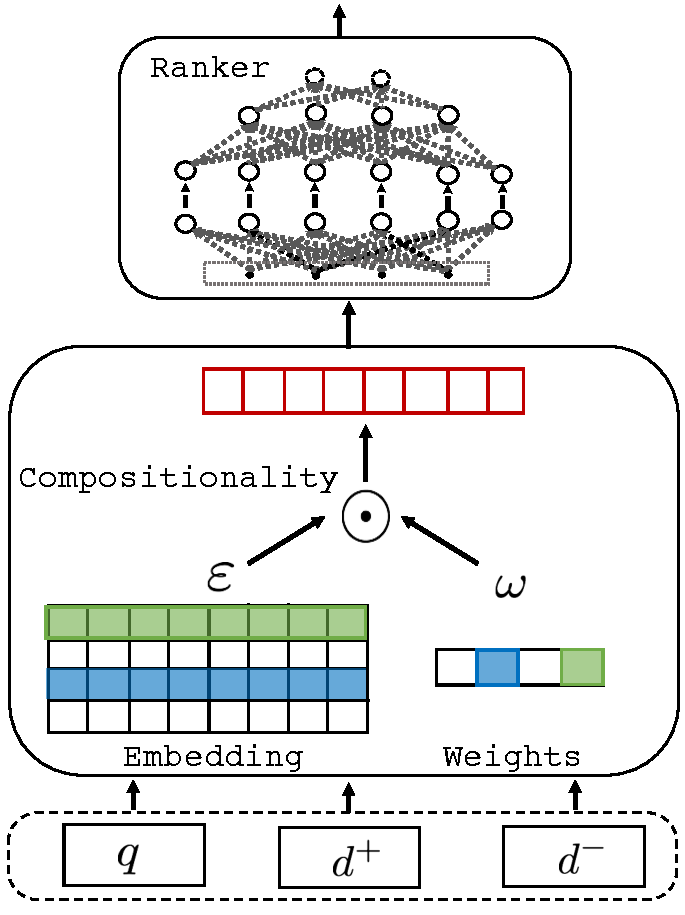
\includegraphics[width=0.35\textwidth]{03-part-02/chapter-05/figs_and_tables/fig_ranker.pdf}
    \caption{The document ranker used as \tch in \cws and \std in \fwl.}
    \label{fig:ranker}
\end{figure}


\subsubsection{The \tnet in \cws and the \std in \fwl}
We employ the pairwise neural ranker architecture explained in Section~\ref{sec:modeltwo} as the \tnet in \cws and \std in \fwl. 

Each training instance $x$ consists of a query $q$, and two documents $d^+$ and $d^-$. The labels, $\tilde{y}$ and $y$, are scalar values indicating the probability of $d^+$ being ranked higher than $d^-$ with respect to $q$.

\mypar{The Representation Learning Layer.}
This layer learns a function $\varepsilon: \mathcal{V} \rightarrow \mathbb{R}^{m}$  (where $\mathcal{V}$ denotes the vocabulary set, and $m$ is the number of embedding dimensions) that maps each word to its embedding which is downstream of the ranking task as well as a weighting function $\omega: \mathcal{V} \rightarrow \mathbb{R}$ which learns the global importance of each word. Then, the learned weights are used to compose word embeddings to generate query/document embeddings. The output of this layer is the concatenation of vectors representing query and two documents.
%
In our experiments, we initialize the embedding function $\varepsilon$ with word2vec embeddings~\cite{Mikolov:2013} pre-trained on Google News and the weighting function $\omega$ with IDF.

\mypar{The Supervision Layer.} 
This layer receives the vector representation of the inputs processed by the representation learning layer and outputs a prediction $\hat{y}_i$.
We opt for a simple fully connected feed-forward network with $l$ hidden layers followed by a sigmoid. We employ the weighted cross entropy loss:
\begin{equation}
% \nonumber
\small
\mathcal{L}_t = \sum_{i\in B_U} \tilde{c}_i [- \tilde{y}_i \log (\hat{y}_i) - (1-\tilde{y}_i) \log(1-\hat{y}_i)],
\end{equation}
where $B_U$ is a batch of instances from $U$, and $\tilde{c}_i$ is the confidence score of the weakly annotated instance $i$, estimated by the \cnet.

The general schema of the \tnet (or \std) is illustrated in Figure~\ref{fig:ranker}. More details are provided in Section~\ref{sec:modeltwo}.

\subsubsection{The \wa}
The \wa in the document ranking task is BM25~\citep{Robertson:2009}, a well-known unsupervised retrieval method. This method heuristically scores a given pair of query-document based on the statistics of their matched terms. In the pairwise document ranking setup, $\tilde{y}_i$ for a given sample $x_j = (q,d^+,d^-)$ is the probability of document $d^+$ being ranked higher than $d^-$: 
$\tilde{y}_i = P_{q,d^+,d^-} = \nicefrac{s_{q,d^+}}{s_{q,d^+} + s_{q,d^-}}$,  where $s_{q,d}$ is the score obtained from the \wa.


\subsubsection{The \cnet in \cws}
The \cnet is a regresses and we use a simple fully connected feed-forward network. To train the \cnet, the target label $c_j$ is calculated using the absolute difference of the strong label and the weak label: $c_j= 1-|y_j - \tilde{y}_j|$, where $y_j$ is calculated similar to $\tilde{y}_i$, but $s_{q,d}$ comes from strong labels provided by humans.


\subsubsection{The \tch in \fwl}
We use Gaussian Process as the \tch in order to generate soft labels. We pass the mean of $\mathcal{GP}$ through the same function $g(.)$ that is applied on the output of the \std network, where the $g(.)$ is sigmoid for the document ranking task.
Since we have one dimensional regression here, $\Sigma(x_t)$ is scalar and $h(.)$ is identity.
In the \tch, linear combinations of different kernels are used. For the document ranking task, we use sparse variational GP regression\footnote{\url{http://gpflow.readthedocs.io/en/latest/notebooks/SGPR_notes.html}}~\citep{Titsias2009variational} with this kernel:
\begin{equation}
k(x_i,x_j)=k_{\rm Matern3/2}(x_i,x_j)+{k_{\rm Linear}}(x_i,x_j)+k_{\rm White}(x_i,x_j)
\end{equation}

where,
\begin{flalign*}
    \hspace{6em}
    &&k_{\rm Matern3/2}(x_i,x_j) &= \left(1+\frac{\sqrt{3}\Vert x_i-x_j\Vert}{l}\right)\exp{\left(-\frac{\sqrt{3}\Vert x_i-x_j\Vert}{l}\right)} & \\
    &&k_{\rm Linear}(x_i,x_j) &= \sigma_0^2+x_i.x_j & \\
    &&k_{\rm White}(x_i,x_j) &= constant\_value, \quad \forall x_1=x_2 \text{ and } 0 \text{ otherwise} & 
\end{flalign*}

We empirically found $l=1$ satisfying value for the length scale of Matern3/2 kernel.
We also set $\sigma_0 = 0$ to obtain a homogeneous linear kernel. 
The constant value of $K_{White}(.,.)$ determines the level of noise in the labels. This is different from the noise in weak labels. This term explains the fact that even in strong labels there might be a trace of noise due to the inaccuracy of human labelers. 

It's noteworthy that we used clustered $\mathcal{GP}$ algorithm, explained in Section~\ref{sec:CGP}, and set the number of clusters to $50$ for this task..  


\subsubsection{Collections}
We use two standard TREC collections for the task of ad-hoc retrieval: The first collection (\emph{Robust04}) consists of 500k news articles from different news agencies as a homogeneous collection. The second collection (\emph{ClueWeb}) is ClueWeb09 Category B, a large-scale web collection with over 50 million English documents, which is considered as a heterogeneous collection. Spam documents were filtered out using the Waterloo spam scorer~\footnote{\url{http://plg.uwaterloo.ca/~gvcormac/clueweb09spam/}}~\citep{Cormack:2011} with the default threshold $70\%$. 

\mypar{Data with strong labels.} 
We take query sets that contain human-labeled judgments: a set of 250 queries (TREC topics 301--450 and 601--700) for the Robust04 collection and a set of 200 queries (topics 1-200) for the experiments on the ClueWeb collection.
For each query, we take all documents judged as relevant plus the same number of documents judged as non-relevant and form pairwise combinations among them.

\mypar{Data with weak labels.}
We create a query set $Q$ using the unique queries appearing in the AOL query logs~\citep{Pass:2006}. 
This query set contains web queries initiated by real users in the AOL search engine that were sampled from a three-month period from March 2006 to May 2006. 
We applied standard pre-processing~\cite{Dehghani:2017:SIGIR,Dehghani2017:CIKM} on the queries: We filtered out a large volume of navigational queries containing URL substrings (``http'', ``www.'', ``.com'', ``.net'', ``.org'', ``.edu''). We also removed all non-alphanumeric characters from the queries. For each dataset, we took queries that have at least ten hits in the target corpus using our \wa method. Applying all these steps, 
We collect 6.15 million queries to train on in Robust04 and 6.87 million queries for ClueWeb.
To prepare the weakly labeled training set $\mathcal{D}_w$, we take the top $1,000$ retrieved documents using BM25 for each query from training query set $Q$, which in total leads to $\sim|Q|\times 10^6$ training samples. 

\subsubsection{Experimental Setup.}
For the evaluation of the whole model, we conducted a 3-fold cross-validation. However, for each dataset, we first tuned all the hyper-parameters of the \tnet in \cws (and \std in the first step of \fwl) in the first step on the set with strong labels using batched GP bandits with an expected improvement acquisition function~\citep{Desautels:2014} and kept the optimal parameters of the \tnet (and \std) fixed for all the other experiments.
The size and number of hidden layers for the \tnet (and \std) is selected from $\{64, 128, 256, 512\}$. The initial learning rate and the dropout parameter were selected from $\{10^{-3}, 10^{-5}\}$ and $\{0.0, 0.2, 0.5\}$, respectively. We considered embedding sizes of $\{300, 500\}$. The batch size in our experiments was set to $128$.  We use ReLU~\citep{Nair:2010} as a non-linear activation function $\alpha$ in \tnet (and \std).  We use the Adam optimizer~\citep{Kingma:2014} for training, and \emph{dropout}~\citep{Srivastava:2014} as a regularization technique.

%
At inference time, for each query, we take the top $2,000$ retrieved documents using BM25 as candidate documents and re-rank them using the trained models. We use the Indri\footnote{\url{https://www.lemurproject.org/indri.php}} implementation of BM25 with default parameters (i.e., $k_1 = 1.2$, $b = 0.75$, and $k_3 = 1,000$).

\subsubsection{Results and Discussions} 
\label{sec:res_and_disc_ranking}
We conducted k-fold cross validation on $\mathcal{D}_s$ (the strong data) and report two standard evaluation metrics for ranking: mean average precision (MAP) of the top-ranked $1,000$
documents and normalized discounted cumulative gain calculated for the top $20$ retrieved documents (nDCG@20). 
Table~\ref{tbl_main} shows the performance on both datasets. As can be seen, \fwl and \cws both provide significant boost on the performance on top of the baseline methods over both datasets.


\input{03-part-02/chapter-05/figs_and_tables/table_ranking_results.tex}

In the ranking task, the \std is designed in particular to be trained on weak annotations~\citep{Dehghani:2017:SIGIR}, hence training the network only on weak supervision, i.e. $\text{NN}_{\text{W}}$ performs better than $\text{NN}_{\text{S}}$. This can be due to the fact that ranking is a complex task requiring many training samples to learn representations that can be used to assess the relevance, while relatively few data with strong labels are available.

Alternating between strong and weak data during training, i.e. $\text{NN}_{\text{W}\text{/S}^+}$ seems to bring little (but statistically significant) improvement. However, we can gain better results by the typical fine-tuning strategies.  Among the fine-tuning experiments, updating all the parameters of the \tnet (or \std), i.e. $\text{NN}_{\text{W}} \to \text{NN}_{\text{S}}$, is the best fine-tuning strategy. Updating only the parameters of the representation layer based on the strong labels, i.e. $\text{NN}_{\text{W}} \to \text{NN}^{\text{Rep}}_{\text{S}}$, works better than updating only parameters of the supervision layer, i.e. $\text{NN}_{\text{W}} \to \text{NN}^{\text{Sup}}_{\text{S}}$. This supports our designed choice of a shared embedding layer in \cws which gets updated on set $V$.

\fwl is the best performing baselines, and \cws achieves 97\% of the performance of \fwl. The main advantage of \cws over \fwl is that it is trained in a single stage process and needs to meet the examples in $\mathcal{D}_w$ (which is a reasonably large set) only one time, while \fwl has three sequential stages during training and it needs to iterate two times over all the examples in $\mathcal{D}_w$. Also employing a Gaussian Process as part of the model in \fwl limits its scalability, while the components of \cws are all neural networks, and this eases the increase in the capacity of the model. 
% With all that, we find \cws a much more efficient model in terms of training cost, with losing little to no performance.


\input{03-part-02/chapter-05/figs_and_tables/table_ranking_res_cws.tex}
As an ablation study on \cws, we tried different training strategies and report the results in Table~\ref{tbl_variants_rank_cws}. As shown, \cws and CWS$_\text{CT}$ perform better than other strategies.
%
\cws$_\text{CT}$ is to let the \cnet to be trained separately, while still being able to enjoy shared learned information from the \tnet. Compared to \cws, \cws$_\text{CT}$ is less efficient as we need two rounds of training on weakly labeled data. 

While it seems reasonable to make use of strong labels for updating \emph{all} parameters of the \tnet, CWS$_\text{JT}^+$ achieves no better results than \cws. We speculate that during training, the direction of the parameter optimization is profoundly affected by the type of supervision signal and while we control the magnitude of the gradients, we do not change their directions. Hence alternating between two sets with different label qualities (different supervision signal types, i.e. weak and strong) confuses the supervision layer of the \tnet. 

In \cws$_\text{ST}$,  the strong dataset, $\mathcal{D}_s$, is too small to train a high-quality \cnet without taking advantage of the vast amount of weakly annotated data in $\mathcal{D}_w$ to learn better representations, so CWS$_\text{ST}$ is not able to improve the performance over $\text{NN}_W$ significantly and also we noticed that this strategy leads to a slow convergence compared to the $\text{NN}_W$. 
Also transferring learned information from \tnet to \cnet via progressive training, i.e., CWS$_\text{PT}$, performs no better than full sharing of the representation learning layer.



\input{03-part-02/chapter-05/figs_and_tables/table_ranking_res_fwl.tex}
Table~\ref{tbl_variants_rank_fwl} presents the results of some experiments we have done as ablation studies on \fwl. 

Weighting the gradient updates from weak labels during pretraining and fine-tuning the network with strong labels, i.e. NN$_{\text{W}^\omega \to \text{S}}$ seems to work quite well.
%
Comparing the performance of \fwlnospace$_{unsuprep}$ to \fwl indicates that, first of all learning the representation of the input data downstream of the main task leads to better results compared to a task-independent unsupervised or self-supervised way. Also the dramatic drop in the performance compared to the \fwl, emphasizes the importance of the preretraining the \std on weakly labeled data.

%
We can gain improvement by fine-tuning the NN$_\text{W}$ using labels generated by the \tch without considering their confidence score, i.e. \fwl$\backslash\Sigma$. This means we just augmented the fine-tuning process by generating a fine-tuning set using \tch which is better than $\mathcal{D}_s$ in terms of quantity and $\mathcal{D}_w$ in terms of quality. This baseline is equivalent to setting $\beta = 0$ in Equation~\ref{eqn:eta2}. However, we see a big jump in performance when we use \fwl to include the estimated label quality from the \tch, leading to the best overall results.

\subsection{Sentiment Classification}
In sentiment classification, the goal is to predict the sentiment (e.g., positive, negative, or neutral) of a sentence. Each training sample $x$ consists of a sentence $s$ and its sentiment label $\tilde{y}$.

\begin{figure}[t!]
    \centering
            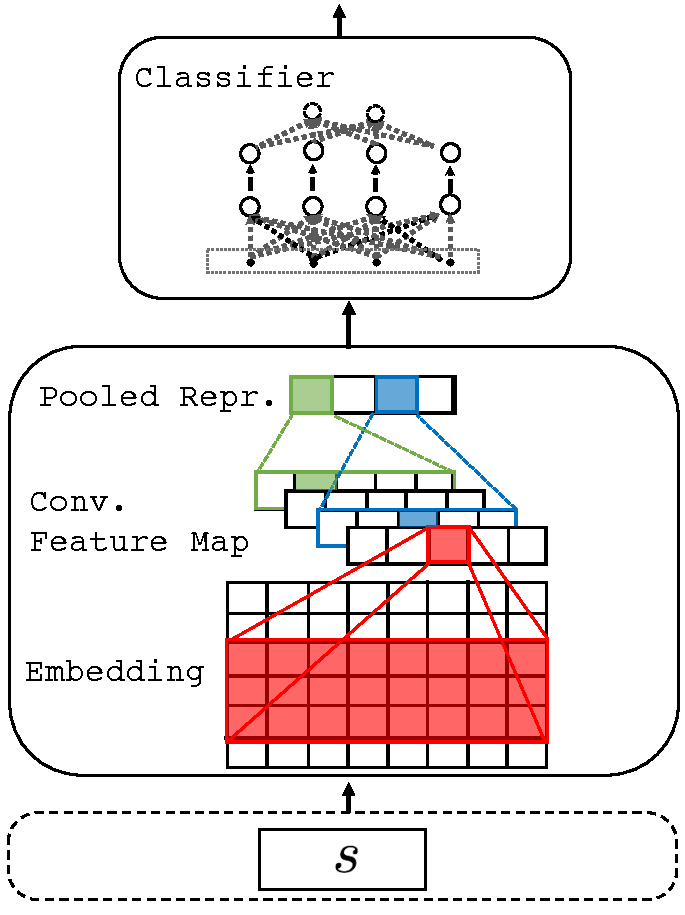
\includegraphics[width=0.35\textwidth]{03-part-02/chapter-05/figs_and_tables/fig_sentiment.pdf}
    \caption{The sentiment classifier used as \tch in \cws and \std in \fwl.}
    \label{fig:sentiment}
\end{figure}


\subsubsection{The \tnet in \cws and the \std in \fwl}
We use a convolutional model~\citep{Kim:2014} as the \tnet in \cws and the \std in \fwl, which is similar to the state-of-the-art model for Twitter sentiment classification from Semeval 2015 and 2016~\cite{Severyn:2015:SemEval,Deriu2016:SemEval,Deriu:2017,Severyn:2015:SIGIR}.

\mypar{The Representation Learning Layer} 
The representation learning layer in this task consists of an embedding function $\varepsilon: \mathcal{V} \rightarrow \mathbb{R}^{m}$, where $\mathcal{V}$ denotes the vocabulary set and $m$ is the number of embedding dimensions.

This function maps the sentence to a matrix $S \in \mathbb{R}^{m \times |s|}$, where each column represents the embedding of a word at the corresponding position in the sentence. We initialize the embedding matrix with word2vec embeddings~\cite{Mikolov:2013} pretrained on a collection of 50M tweets.

Matrix $S$ is passed through a convolution layer.  In this layer, a set of $f$ filters is applied to a sliding window of length $h$ over $S$ to generate a feature map matrix $O$. Each feature map $o_i$ for a given filter $F$ is generated by $o_i = \sum_{k,j}S[i:i+h]_{k,j} F_{k,j}$, where $S[i:i+h]$ denotes the concatenation of word vectors from position $i$ to $i+h$. The concatenation of all $o_i$ produces a feature vector $o \in \mathbb{R}^{|s|-h+1}$. The vectors $o$ are then aggregated over all $f$ filters into a feature map matrix $O \in \mathbb{R}^{f\times(|s|-h+1)}$.

We also add a bias vector $b \in R^f$ to the result of a convolution.
Each convolutional layer is followed by a non-linear activation function (we use ReLU\cite{Nair:2010}) which is applied element-wise. Afterward, the output is passed to the max pooling layer which operates on columns of the feature map matrix $O$ returning the largest value: $pool(o_i) : \mathbb{R}^{1\times(|s|-h+1)} \rightarrow \mathbb{R}$.

\mypar{The Supervision Layer.} 
This layer is a simple fully connected feed-forward network with $l$ hidden layers, followed by a softmax.  We employ the weighted cross entropy loss:
\begin{equation}
% \nonumber
\mathcal{L}_t = \sum_{i\in B_U} \tilde{c}_i \sum_{k \in K} - \tilde{y}_i^k \log (\hat{y}_i^k),
\end{equation}
where $B_U$ is a batch of instances from $U$, and $\tilde{c}_i$ is the confidence score of the weakly annotated instance $i$, and $K$ is a set of classes. 
The general schema of the \tnet (or \std) is illustrated in Figure~\ref{fig:sentiment}.

\subsubsection{The \wa}
\label{sentiment-WA}
The \wa for the sentiment classification task is a simple lexicon-based method~\citep{Hamdan:2013,Kiritchenko:2014}.
We use SentiWordNet03~\citep{Gaccianella:2010} to assign probabilities (positive, negative and neutral) for each token in set $\mathcal{D}_w$. We use a bag-of-words model for the sentence-level probabilities (i.e.\ just averaging the distributions of the terms), yielding a noisy label $\tilde{y}_i \in \mathbb{R}^{|K|}$, where $|K|=3$ is the number of classes.  We found empirically that using soft labels from the \wa works better than assigning a single hard label.


\subsubsection{The \cnet in \cws}
In this task, the \cnet is also a regresses and we use a simple fully connected feed-forward network. The target label $c_j$ for the \cnet is calculated by using the mean absolute difference of the strong label and the weak label: $c_j= 1-\frac{1}{|K|}\sum_{k\in K}|y_j^k - \tilde{y}_j^k|$, where $y_j$ is the one-hot encoding of the sentence label over all classes.


\subsubsection{The \tch in \fwl}
Similar to the ranking task, we use Gaussian Process as the \tch in order to generate soft labels. We pass the mean of $\mathcal{GP}$ through the same function $g(.)$ that is applied on the output of the \std network, where the $g(.)$ is softmax for the sentiment classification task.
Here in this task, $h(.)$ is an aggregation function that takes variance over several dimensions and outputs a single measure of variance. As a reasonable choice, the aggregating function $h(.)$ in the sentiment classification task (three classes) is \emph{mean} of variances over dimensions. 
In the \tch, linear combinations of different kernels are used. For the sentiment classification task, We use sparse variational GP for multiclass classification\footnote{\url{http://gpflow.readthedocs.io/en/latest/notebooks/multiclass.html}}~\citep{hensman2014scalable} with the following kernel:
\begin{equation}
k(x_i,x_j)=k_{\rm RBF}(x_i,x_j)+{k_{\rm Linear}}(x_i,x_j)+k_{\rm White}(x_i,x_j)
\end{equation}
where,
\begin{flalign*}
    \hspace{6em}
    &&k_{\rm RBF}(x_i,x_j) &= \exp{\left(\frac{\Vert x_i-x_j\Vert^2}{2l^2}\right)} & 
    \\
    &&k_{\rm Linear}(x_i,x_j) &= \sigma_0^2+x_i.x_j & \\
    &&k_{\rm White}(x_i,x_j) &= constant\_value, \quad \forall x_1=x_2 \text{ and } 0 \text{ otherwise} & 
\end{flalign*}

Similar to the ranking task, we set $l=1$ the length scale of RBF kernel, set $\sigma_0 = 0$  for the linear kernel, and set the number of clusters to $30$ in clustered $\mathcal{GP}$ algorithm.


\subsubsection{Collections}
We test our model on the twitter message-level sentiment classification of SemEval-15 Task 10B \citep{rosenthal:2015}. Datasets of SemEval-15 subsume the test sets from previous editions of SemEval, i.e. SemEval-13 and SemEval-14. Each tweet was preprocessed so that URLs and usernames are masked.

\mypar{Data with strong labels.} 
We use train (9,728 tweets) and development (1,654 tweets) data from SemEval-13 for training and SemEval-13-test (3,813 tweets) for validation.
To make your results comparable to the official runs on SemEval we us SemEval-14 (1,853 tweets) and  SemEval-15 (2,390 tweets) as test sets~\citep{rosenthal:2015, Nakov:2016}.

\mypar{Data with weak labels.}
We use a large corpus containing 50M tweets collected during two months for both, training the word embeddings and creating the weakly annotated set $\mathcal{D}_w$ using the lexicon-based method explained in Section~\ref{sentiment-WA}. 

\subsubsection{Experimental Setup.}
Similar to the document ranking task, we tuned hyper-parameters for the \tnet in \cws (and \std in the first step of \fwl) with respect to the strong labels of the validation set using batched GP bandits with an expected improvement acquisition function~\citep{Desautels:2014} and kept the optimal parameters fixed for all the other experiments.  
The size and number of hidden layers for the classifier and is selected from $\{32, 64, 128\}$.
We tested the model with both, $1$ and $2$ convolutional layers. The number of convolutional feature maps and the filter width is selected from $\{200,300\}$ and $\{ 3, 4, 5\}$, respectively. The initial learning rate and the dropout parameter were selected from $\{1E-3, 1E-5\}$ and $\{0.0, 0.2, 0.5\}$, respectively. We considered embedding sizes of $\{100, 200\}$ and the batch size in these experiments was set to $64$. ReLU~\citep{Nair:2010} is used as a non-linear activation function in \tnet (and \std).  Adam optimizer~\citep{Kingma:2014} is used for training, and \emph{dropout}~\citep{Srivastava:2014} as a regularizer.

In the rest of the chapter, we will present the main results of the introduced baseline methods and the proposed models, \cws and \fwl, 


\subsubsection{Results and Discussions} 
\input{03-part-02/chapter-05/figs_and_tables/table_sentiment_results.tex}
We report Macro-F1, the official SemEval metric, in Table~\ref{tbl_main_sent}. 

Among all the baselines, \fwl is the best performing approach. \cws is also outperforms all the baselines. 

For this task, since the amount of data with strong labels are larger compared to the ranking task, the performance of $\text{NN}_{\text{S}}$ is acceptable. Alternately sampling from weak and strong data, i.e.  $\text{NN}_{\text{W}\text{/S}^+}$ gives better results than either of learning from just weak or just strong labels. However, pretraining on weak labels then fine-tuning both the supervision layer and the representation learning layer on strong labels, further improves the performance.  

Besides the baselines, we also report the best performing systems which are also convolution-based models (\citealt{Rouvier:2016} on SemEval-14; \citealt{Deriu2016:SemEval} on SemEval-15). Both \cws and \fwl outperform these methods.


\input{03-part-02/chapter-05/figs_and_tables/table_sentiment_res_cws.tex}
Similar to the ranking task, we have done an ablation study on \cws by trying different strategies for training \cws. The results of these experiments are presented in Table~\ref{tbl_variants_sent_cws}. \cws$_\text{CT}$ archives the highest performance among all the training strategies, however, as we discussed in Section~\ref{sec:res_and_disc_ranking}, it is not as efficient as \cws. 

In sentiment classification, compared to the ranking task, it is easier to estimate the confidence score of instances concerning the amount of available supervised data. Therefore, \cws$_\text{ST}$ improves the performance over $\text{NN}_{\text{S}}$ in Table~\ref{tbl_main_sent}. 


\input{03-part-02/chapter-05/figs_and_tables/table_sentiment_res_fwl.tex}
The results of a set of experiments we have done as ablation studies on \fwl is presented Table~\ref{tbl_variants_sent_fwl}. 

Having static weighting on the gradient updates, i.e. NN$_{\text{W}^\omega \to \text{S}}$, leads to the performance that is better than simple fine-tuning, i.e. $\text{NN}_{\text{W}} \to \text{NN}_{\text{S}}$ in Table~\ref{tbl_main_sent} .
%
For this task, similar to the ranking task, learning the representation in an unsupervised task independent fashion, i.e. \fwlnospace$_{unsuprep}$, does not lead to good results compared to the \fwl.
%
Similar to the ranking task, fine-tuning $\text{NN}_{\text{W}}$ based on labels generated by $\mathcal{GP}$ instead of data with strong labels, regardless of the confidence score, i.e. \fwl$\backslash\Sigma$, works better than standard fine-tuning. 

\section{Discussion and Analysis}
\label{sec:discussion}
\shrink
In this section, we provide further analysis by investigating the learning pace in \cws and \fwl, bias-variance trade-off in \fwl, sensitivity of \fwl to the quality of weak labels, and how modifying the learning rate in \fwl can be different from weighted sampling of training examples.

\subsection{Faster Learning Pace in \cws}
\label{sec:learning_pace}
\begin{figure}[!t]%
    \centering
    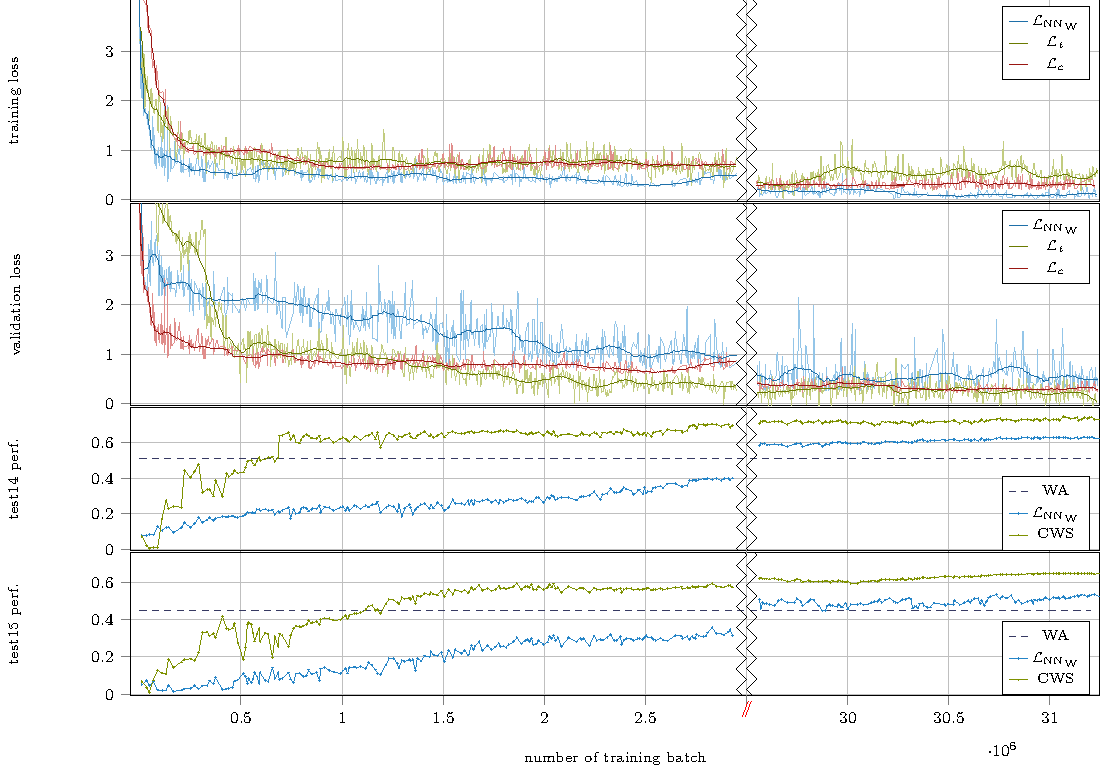
\includegraphics[width=0.8\textwidth]{03-part-02/chapter-05/figs_and_tables/plot_loss_cws.pdf}
    \caption{Loss of the \tnet ($\mathcal{L}_t$) and the \cnet ($\mathcal{L}_c$) compared to the loss of $\text{NN}_{\text{W}}$ ($\mathcal{L}_{\text{NN}_{\text{W}}}$) on training/validation set and performance of \cws, $\text{NN}_{\text{W}}$, and \wa on test sets with respect to different amount of training data on sentiment classification.}
    \label{fig:plot_loss_cws}
\end{figure}
In \cws, controlling the contribution of the weak labels on updating the parameters of the model not only improves the performance, but also provides the network with more solid signals which speeds up the learning process. 

Figure~\ref{fig:plot_loss_cws} illustrates the training/validation loss for both networks compared to the loss of training the \tnet with weak supervision, along with their performance on test sets, with respect to different amounts of training data for the sentiment classification task.
As shown, in training, the loss of the \tnet in our model, i.e., $\mathcal{L}_t$ is higher than the loss of the network which is trained only on weakly supervised data, i.e., $\mathcal{L}_{\text{NN}_{\text{W}}}$. 
%
However, since these losses are calculated with respect to the weak labels (not true labels), having very low training loss can be an indication of overfitting to the imperfection in the weak labels. 
%
In other words, regardless of the general problem of lack of generalization due to overfitting, in the setup of learning from weak labels, predicting labels that are similar to train labels (very low training loss) is not necessarily a desirable incident. 

In the validation set, however, $\mathcal{L}_t$ decreases faster than $\mathcal{L}_{\text{NN}_{\text{W}}}$, which supports the fact that $\mathcal{L}_{\text{NN}_{\text{W}}}$ overfits to the imperfection of weak labels, while our setup helps the \tnet to escape from this imperfection and do an excellent job on the validation set.
%
In terms of the performance, compared to $\text{NN}_{\text{W}}$, the performance of CWS on both test sets increases very quickly and CWS can pass the performance of the \wa by seeing much fewer instances annotated by the \wa.
\subsection{A Good Teacher is Better Than Many Observations} 

We also look at the rate of learning for the \std in \fwl as the amount of training data is varied. We performed two types of experiments for all tasks:
%
\begin{itemize}
    \item In the first experiment, we use all the available strong data but consider different percentages of the entire weak dataset.
    \item In the second experiment, we fix the amount of weak data and provide the model with varying amounts of strong data.
\end{itemize} 
We use standard fine-tuning with similar setups as for the baseline models. 
We fixed everything in the model and tried running the fine-tuning step with different values for $\beta \in \{0.0, 0.1, 1.0, 2.0, 5.0\}$ in all the experiments.
For the experiments on toy problem in Section~\ref{sec:learning_pace}, the reported numbers are averaged over 10 trials. In the first experiment (i.e. Figure~\ref{fig:plot_dw}), the size of sampled data data is: $|\mathcal{D}_s| = 50$ and $|\mathcal{D}_w| = 100$ (Fixed) and for the second one (i.e. Figure~\ref{fig:plot_dw}): $|\mathcal{D}_w| = 100$ and $|\mathcal{D}_s| = 10$ (fixed). 

Figure~\ref{fig:learning_rate} presents the results of these experiments. In general, for all tasks and both setups, the \std learns faster when there is a \tch.
One caveat is in the case where we have a very small amount of weak data. In this case the \std cannot learn a suitable representation in the first step, and hence the performance of \fwl is pretty low, as expected. It is highly unlikely that this situation occurs in reality as obtaining weakly labeled data is much easier than strong data.

The empirical observation of Figure~\ref{fig:learning_rate} that our model learns more with less data can also be seen as evidence in support of another perspective to \fwl, called \emph{learning using privileged information}~\citep{vapnik2015learning} which we explained in Section~\ref{sec:LUPI}. 
\input{03-part-02/chapter-05/figs_and_tables/plot_learning_rate.tex}


\subsection{Handling the Bias-Variance Trade-off in \fwl}
\label{sec:bias-variance}
As mentioned in Section~\ref{sec:proposed-method}, $\beta$ is a hyperparameter that controls the contribution of weak and strong data to the training procedure. In order to investigate its influence, we fixed everything in the model and ran the fine-tuning step with different values of $\beta \in \{0.0, 0.1, 1.0, 2.0, 5.0\}$ in all the experiments.

%
\begin{figure}[t]
    \centering
    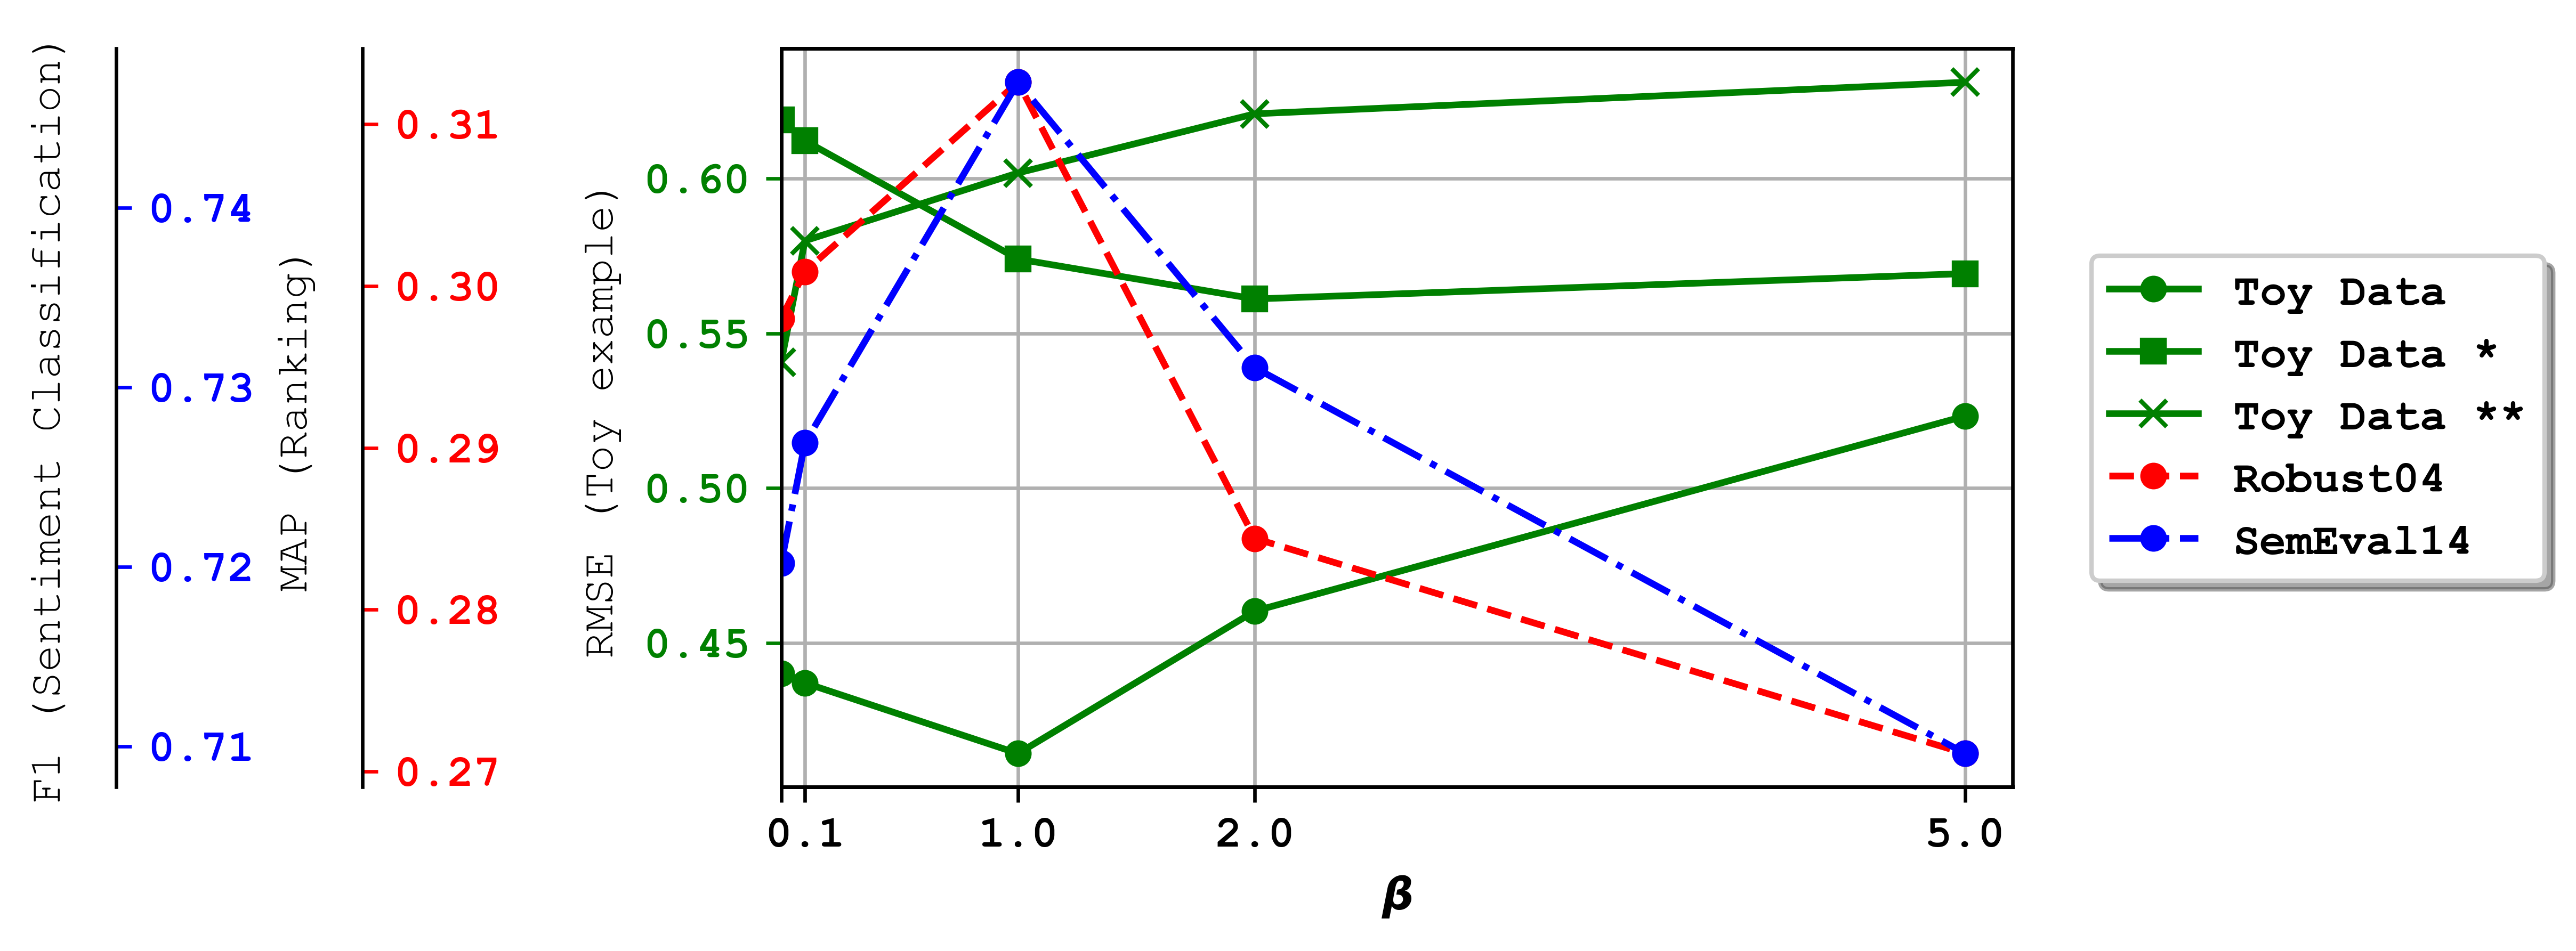
\includegraphics[width=0.7\textwidth]{03-part-02/chapter-05/figs_and_tables/plot_beta_fwl.png}
    \caption{Effect of different values for $\beta$.}
    \label{fig:beta}
\end{figure}

Figure~\ref{fig:beta} illustrates the performance on the ranking (on Robust04 dataset) and sentiment classification tasks (on SemEval14 dataset).  For both sentiment classification and ranking, $\beta=1$ gives the best results (higher scores are better).
%
We also experimented on the toy problem with different values of $\beta$ in three cases: 
1) having 10 observations from the true function (same setup as Section~\ref{sec:toy_exmpale}), marked as ``Toy Data'' in the plot, 
2) having only 5 observations from the true function, marked as ``Toy Data *'' in the plot, and 
3) having $f(x) = x + 1$ as the weak function, which is an extremely bad approximator of the true function, marked as ``Toy Data **'' in the plot.
%
For the ``Toy Data'' experiment, $\beta=1$ turned out to be optimal (here, lower scores are better). However, for ``Toy Data *'', where we have an extremely small number of observations from the true function, setting $\beta$ to a higher value acts as a regularizer by relying more on weak signals, and eventually leads to better generalization. 
On the other hand, for ``Toy Data **'', where the quality of the \wa is extremely low, lower values of $\beta$ put more focus on the true observations. Therefore, $\beta$ lets us control the bias-variance trade-off in these extreme cases.

We have also tested $\hat{c}_t = \eta_2(x_t) = \nicefrac{\beta}{\rm var}[\Sigma(x_t)]$.  The experiments showed that the exponential choice gives a better overall performance. 


\subsection{Sensitivity of the \fwl to the Quality of the Weak Annotator}
Our proposed setup in \fwl requires defining a so-called ``\wa'' to provide a source of weak supervision for unlabelled data. In Section~\ref{sec:bias-variance} we discussed the role of parameter $\beta$ for controlling the bias-variance trade-off by trying two weak annotators for the toy problem. 
Now, in this section, we study how the quality of the weak annotator may affect the performance of the \fwl, for the task of document ranking as a real-world problem.

To do so, besides BM25~\citep{Robertson:2009}, we use three other weak annotators: 
\begin{figure}[t]
    \centering
    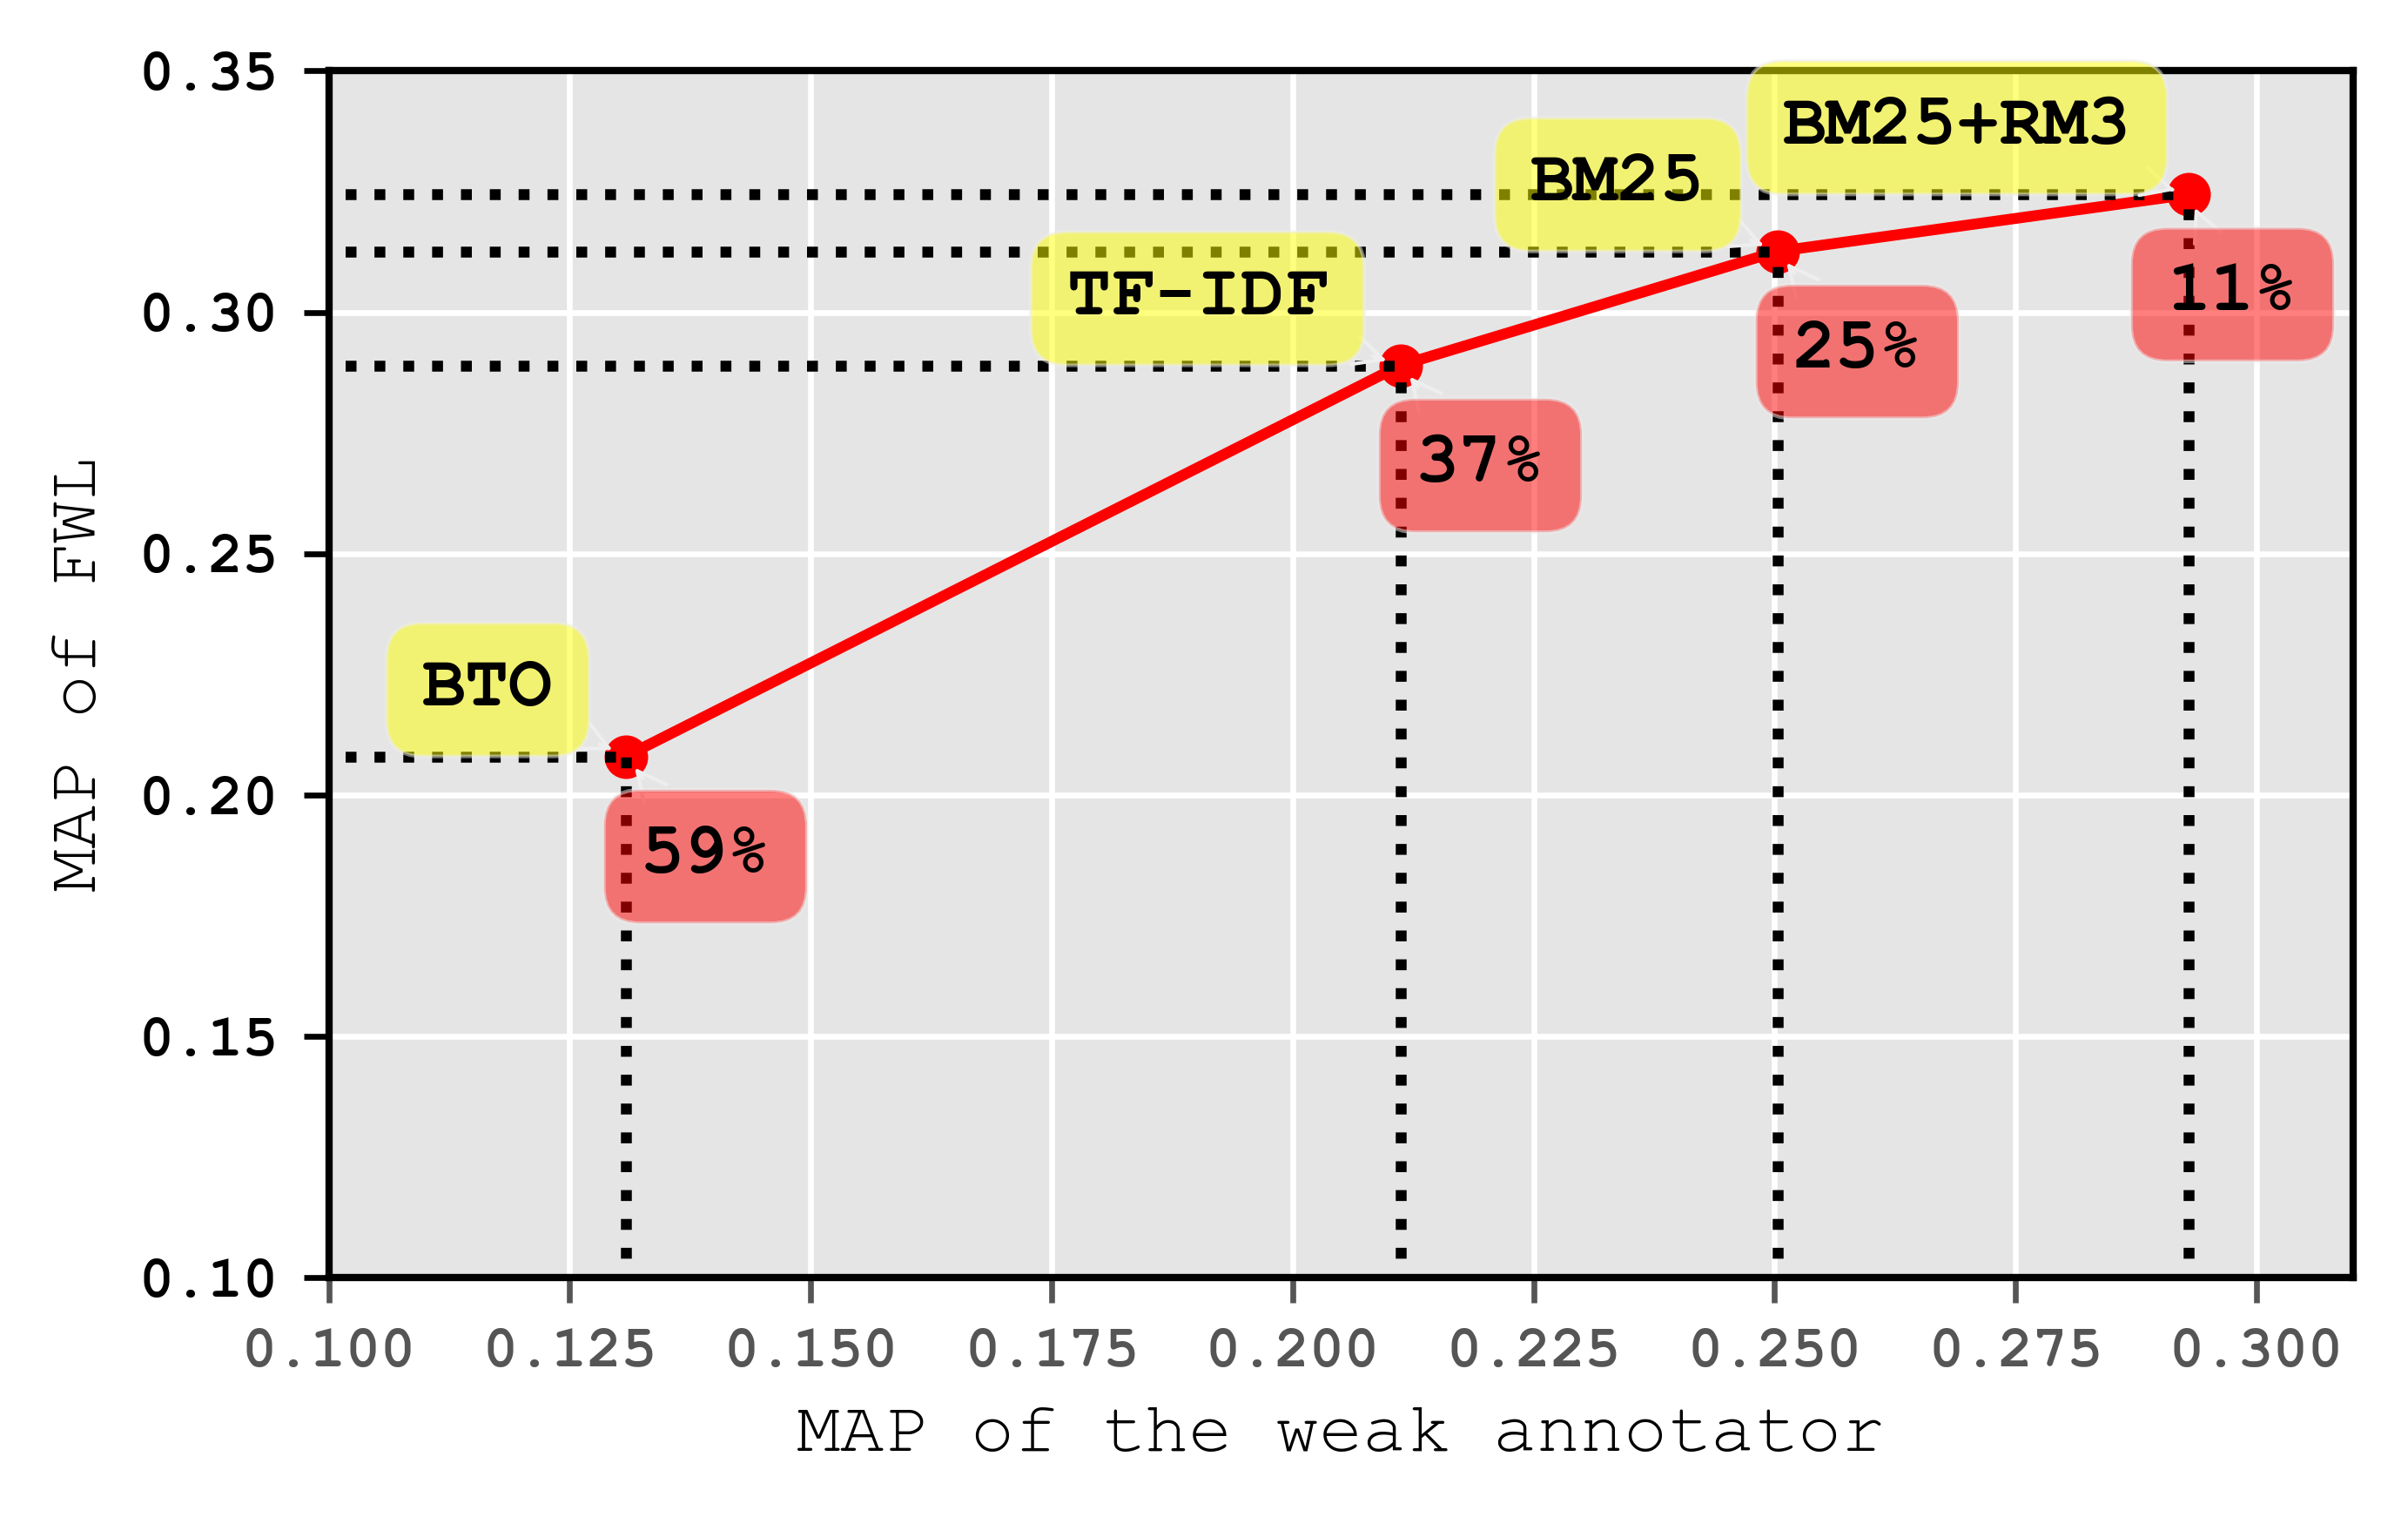
\includegraphics[width=0.7\textwidth]{03-part-02/chapter-05/figs_and_tables/plot_sensitivity_fwl.png}
    \caption{Performance of \fwl versus performance of the corespondence \wa in the document ranking task, on Robust04 dataset.}
    \label{fig:sensitivity}
\end{figure}
vector space model~\citep{salton1973specification} with binary term occurrence (BTO) weighting schema and vector
space model with TF-IDF weighting schema, which are both weaker than BM25, 
and BM25+RM3~\citep{Abdul-jaleel:2004} that uses RM3 as the pseudo-relevance feedback method on top of BM25, leading to better labels. 

Figure~\ref{fig:sensitivity} illustrates the performance of these four \was in terms of their mean average precision (MAP) on the test data, versus the performance of \fwl given the corresponding \wa. As it is expected, the performance of \fwl depends on the quality of the employed \wa.
The percentage of improvement of \fwl over its corresponding \wa on the test data is also presented in Figure~\ref{fig:sensitivity}. As can be seen, the better the performance of the \wa is, the less the improvement of the \fwl would be. 


\subsection{From Modifying the Learning Rate to Weighted Sampling}
\fwl provides confidence score based on the certainty associated with each generated label $\bar{y}_t$, given sample $x_t \in \mathcal{D}_{sw}$. We can translate the confidence score as how likely including $(x_t,\bar{y}_t)$ in the training set for the \std model improves the performance, and rather than using this score as the multiplicative factor in the learning rate, we can use it to bias sampling procedure of mini-batches so that the frequency of training samples are proportional to the confidence score of their labels.

We design an experiment to try \fwl with this setup (\fwlnospace$_s$), in which we keep the architectures of the \std and the \tch and the procedure of the  first two steps of the \fwl fixed, but we changed the step 3 as follows:

Given the soft dataset $\mathcal{D}_{sw}$, consisting of $x_t$, its label $\bar{y}_t$ and the associated confidence score generated by the \tch, we normalize the confidence scores over all training samples and set the normalized score of each sample as its probability to be sampled. 
Afterward, we train the \std model by mini-batches sampled from this set with respect to the probabilities associated with each sample, but without considering the original confidence scores in parameter updating.
This means the more confident the \tch is about the generated label for each sample, the more chance that sample has to be seen by the \std model.
\begin{figure}[t]
    \centering
    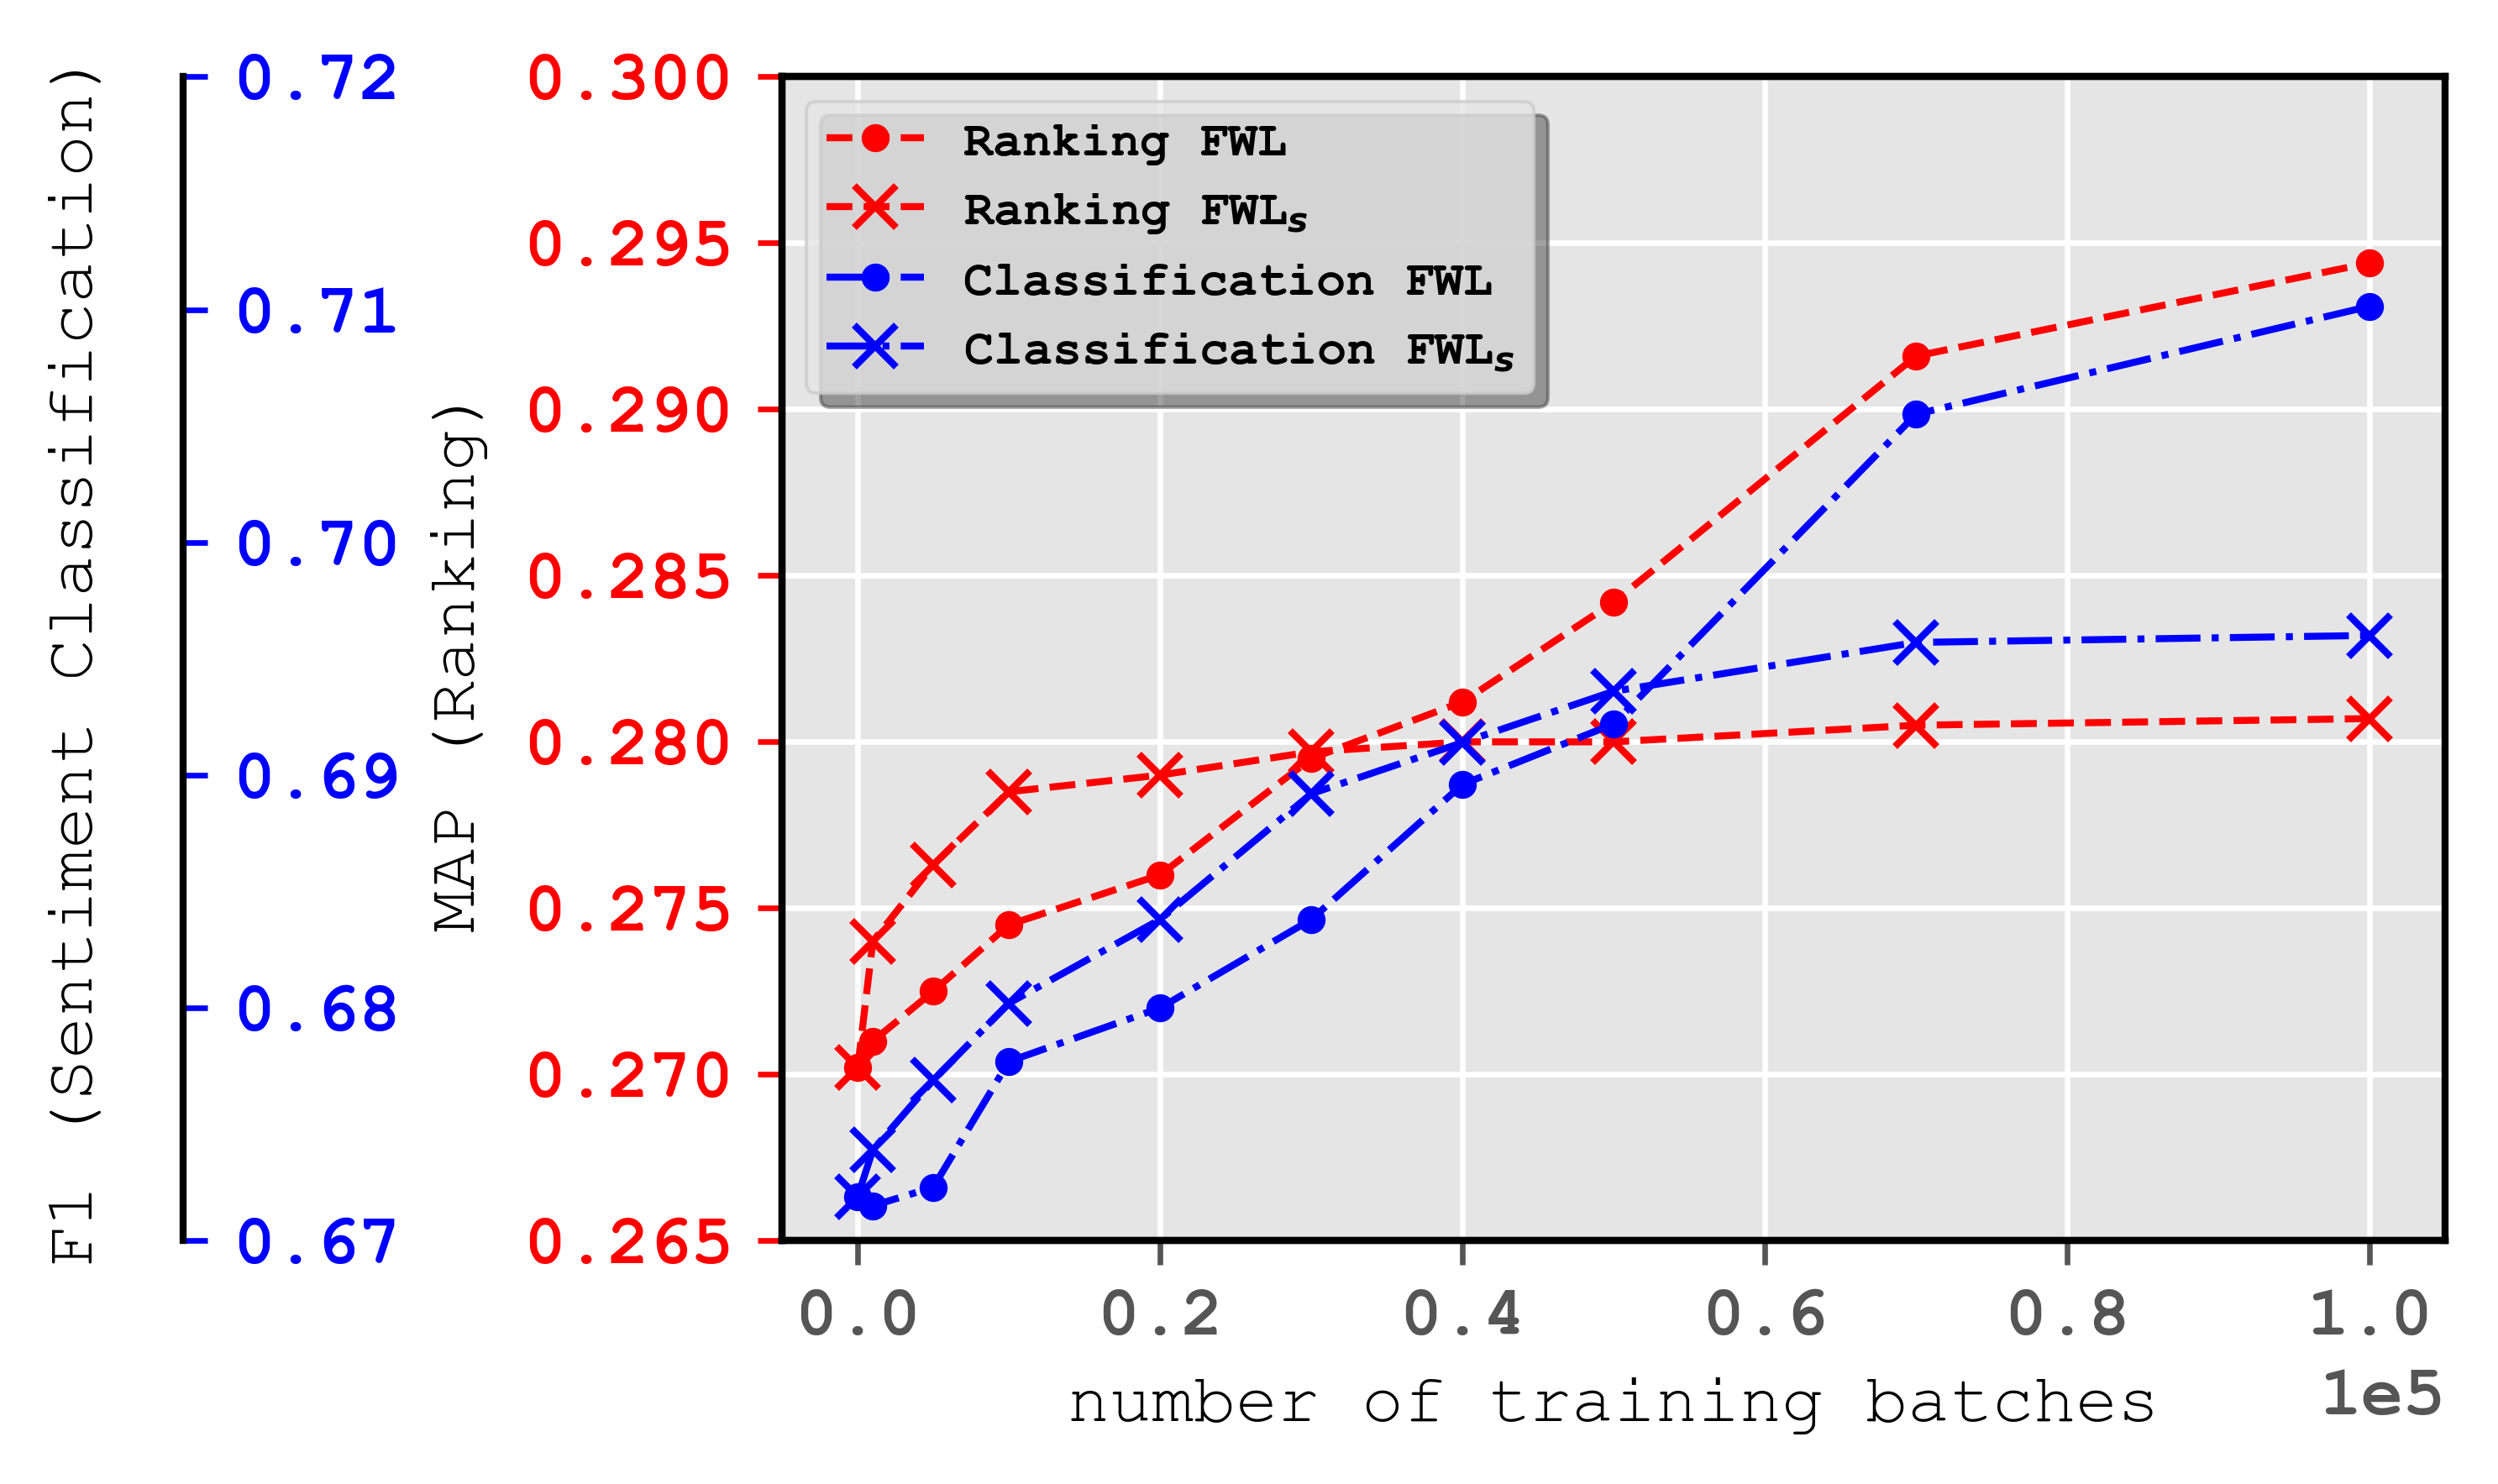
\includegraphics[width=0.7\textwidth]{03-part-02/chapter-05/figs_and_tables/plot_sampling_fwl.png}
    \caption{Performance of \fwl and \fwlnospace$_s$ with respect to different batch of data for the task of document ranking (Robust04 dataset) and sentiment classification (SemEval14 dataset).}
    \label{fig:sampling}
\end{figure}
Figure~\ref{fig:sampling} illustrates the performance of both \fwl and \fwlnospace$_s$ trained on different amount of data sampled from $\mathcal{D}_{sw}$, in the document ranking and sentiment classification tasks. 

As can be seen, compared to \fwl, the performance of \fwlnospace$_s$ increases rapidly in the beginning but it slows down afterward. 
We have looked into the sampling procedure and noticed that the confidence scores provided by the \tch form a rather skewed distribution and there is a strong bias in \fwlnospace$_s$ toward sampling from data points that are either in or closed to the points in $\mathcal{D}_{s}$, as $\mathcal{GP}$ has less uncertainty around these points and the confidence scores are high.
We observed that the performance of \fwlnospace$_s$ gets closer to the performance of \fwl after many epochs, while \fwl had already a log convergence.
%
The skewness of the confidence distribution makes \fwlnospace$_s$ to have a tendency for more exploitation than exploration, however, \fwl has more chance to explore the input space, while it controls the effect of updates on the parameters for samples based on their merit. 




\section{Related Work}
\label{sec:relatedwork}
In this section, we position the introduced \cws and \fwl approaches relative to related work.

\subsection{Learning from Imperfect Data}
Learning from imperfect labels has been thoroughly studied in the literature~\citep{Frenay:2014}.  The imperfect (weak) signal can come from non-expert crowd workers,  be the output of other models that are weaker (for instance with low accuracy or coverage), biased, or models trained on data from different related domains. 
%
Among these forms, in the distant supervision setup, a heuristic labeling rule~\citep{Deriu2016:SemEval,Severyn:2015:SemEval} or function~\citep{Dehghani:2017:SIGIR} which can be relying on a knowledge base~\citep{Mintz2009:distant,  min2013distant, Han:2016} is employed to devise noisy labels.  

Learning from weak data sometimes aims at encoding various forms of domain expertise or cheaper supervision from lay annotators. For instance, in the structured learning, the label space is pretty complex and obtaining a training set with strong labels is extremely expensive, hence this class of problems leads to a wide range of works on learning from weak labels~\citep{roth2017incidental}. 
%
Indirect supervision is considered as a form of learning from weak labels that is employed in particular in the structured learning, in which a companion binary task is defined for which obtaining training data is easier~\citep{Chang2010structured, Raghunathan:2016}. 

In the response-based supervision, the model receives feedback from interacting with an environment in a
task, and converts this feedback into a supervision
signal to update its parameters~\citep{roth2017incidental,clarke2010driving,riezler2014response}.
%
Constraint-based supervision is another form of weak supervision in which constraints that are represented as weak label distributions are taken as signals for updating the model parameters. For instance, physics-based constraints on the output~\citep{stewart2017label} or output constraints on execution of logical forms~\citep{clarke2010driving}.

In the proposed \cws and \fwl, we can employ these approaches as the weak annotator to provide imperfect labels for the unlabeled data, however, a small amount of data with strong labels is also needed, which put our model in the class of semi-supervised models. 

Some noise cleansing methods have been proposed to remove or correct mislabeled samples~\citep{Brodley:1999}.
There are some studies showing that weak or noisy labels can be leveraged by modifying the loss function~\citep{reed2014training, Patrini:2016, patrini2016loss, Vahdat:2017} or changing the update rule to avoid imperfections of the noisy data~\citep{malach2017decoupling, Dehghani:2017:nips_metalearn, Dehghani:2017avoiding}.  

One direction of research focuses on modeling the pattern of the noise or weakness in the labels. For instance, methods that use a generative model to correct weak labels such that a discriminative model can be trained more effectively~\citep{Ratner:2016,Rekatsinas:2017,Varma:2017}.
Furthermore, methods that aim at capturing the pattern of the noise by inserting an extra layer~\citep{goldberger2016training} or a separate module tries to infer better labels from noisy ones and use them to supervise the training of the network~\citep{Sukhbaatar:2014,Veit:2017, Dehghani:2017:nips_metalearn}. Our proposed \fwl can be categorized in this class as the \tch tries to infer better labels and provide certainty information which is incorporated as the update rule for the \std model.

\subsection{Semi-\:supervised Learning}
In the semi-supervised setup, some ideas were developed to utilize weakly or even unlabeled data. For instance, the idea of self(incremental)-training~\citep{Rosenberg:2005}, pseudo-labeling~\citep{Lee:2013,Hinton:2015}, and Co-training~\citep{Blum:1998} are introduced for augmenting the training set by unlabeled data with predicted labels.
Some research used the idea of self-supervised (or unsupervised) feature learning~\citep{noroozi2016unsupervised,dosovitskiy2016discriminative,donahue2016adversarial} to exploit different labelings that are freely available besides or within the data, and to use them as intrinsic signals to learn general-purpose features. These features, that are learned using a proxy task, are then used in a supervised task like object classification/detection or description matching.

As a common approach in semi-supervised learning, the unlabeled set can be used for learning the distribution of the data. In particular for neural networks, greedy layer-wise pre-training of weights using unlabeled data is followed by supervised fine-tuning~\citep{Hinton:2006,Deriu:2017,Severyn:2015:SemEval,Severyn:2015:SIGIR,Go:2009}. Other methods learn unsupervised encoding at multiple levels of the architecture jointly with a supervised signal~\citep{Ororbia:2015,Weston:2012}.


\subsection{Sentiment Classification and Document Ranking}
Sentiment classification is one of the key NLP tasks and SemEval provides standard benchmark datasets for this task~\citep{rosenthal:2015,Nakov:2016,rosenthal2017semeval}. There are many models proposed based on neural networks for sentiment classification task and in many datasets, the SOTA results are from convolutional-based models that learn multiple word vector representations~\citep{Kim:2014}. In our work, we adapt the CNN based architecture which is proposed to be trained with the help of weak (distance) supervising~\citep{Severyn:2015:SIGIR,Severyn:2015:SemEval,Deriu2016:SemEval} and has achieved SOTA results in some SemEval datasets~\citep{Deriu:2017}.
%
Document Ranking is also the core task of IR and some recent studies have applied neural networks on this task. Two main groups of models are those that learn representation for query and documents, independently,  and then use a matching function~\citep{Huang:2013,Mitra:2017,Shen:2014}, or models that try to capture interaction between query and document from the beginning~\citep{Lu:2013,Guo:2016,Dehghani:2017:SIGIR,Xiong:2017}. Here, we adapt a neural ranker with SOTA results that uses weak supervision~\citep{Dehghani:2017:SIGIR,dehghani:2018:ICLR}.



\section{Conclusion}
Training neural networks using large amounts of weakly annotated data is an attractive approach in scenarios where an adequate amount of data with true labels is not available, a situation which often arises in practice.
%
In this chapter, to address \textbf{\resqname{c5}}, we introduced two semi-supervised learning approaches in the presence of weakly labeled data: Learning from Controlled Weak Supervision (\cws) and \fwlfulllc (\fwl).

\cws is a meta-learning approach that we proposed to address \textbf{\resqname{c5.1}}. It unifies learning to estimate the confidence score of weak annotations and training neural networks to learn a target task with controlled weak supervision, i.e., using weak labels to updating the parameters but taking their estimated confidence scores into account. This helps to alleviate updates from instances with unreliable labels that may harm the performance.

\fwl is a student-teacher framework that we proposed to address \textbf{\resqname{c5.2}}. In \fwl the student network is in charge of learning a target task given a vast amount of samples with weak labels associated with fidelity scores that are generated by the teacher network. In \fwl, we pretrain the student network on weak data to learn an initial task-dependent data representation, which we pass to the teacher along with the strong data. The teacher then learns to predict the strong data, but crucially, \emph{based on the student's learned representation}. This then allows the teacher to generate new labeled training data from unlabeled data as well as fidelity scores for each sample in the data. Using samples in the new dataset, we update the parameters of the student network taking the fidelity scores into account to modulate the learning rate. 

We applied both \cws and \fwl to document ranking and sentiment classification, and empirically verified that they improve over state-of-the-art semi-supervised alternatives and speeds up the training process. We observed that the common approach of pre-training and fine-tuning is not as effective and found that explicitly modeling label quality is both possible and useful in this situation. 

\bigskip
%conclusion of part 2 and connection to part 3
In part~\ref{part2} to address \textbf{\resqname{p2}}, we explored different ideas for developing models that are capable of learning from weakly annotated data. We start with exploring how different architectural choices and different objective functions can be employed for learning with pseudo-labels that are programatically generated to augment training data. Then we study how to metal-learn the quality of labels and how to incorporate them in the learning process.
%
In the next part, we study how we can employ inductive biases as modeling assumptions to design models that are not effective, but also data-efficient.
% !TEX root = ../thesis-main.tex
\part{\titleof{p3}}
\label{part3}
Generalization is at the heart of many aspects of human cognition. It underlies our ability to learn language, form and use categories, and learn about causal relationships, while in many cases we are presented only with limited observation. The great ability of generalization in human cognition sets a standard to which artificial intelligence and machine learning research aspires.

This immediately raises questions like ``How can human learn so much about the world from such limited evidence?'' and ``What makes human so good at generalization?''.
The importance of generalization in cognitive science partly derives
from its close relationship to inductive inference.  We can define generalization as forming predictions about future events based on examples from the past, which emphasizes its relationship to the classic problem of induction~\citep{hume2003treatise}. 
Having this connection between generalization and induction in mind, we can cast the question of ``how to produce good generalizations?'' to the question of ``what makes a good inductive learner?''.

To answer this question from a human cognition perspective, as human develop, they become capable of exploring ``more sophisticated hypotheses'' about the structure of their environment~\citep{inhelder1958growth}, which allows them to better infer their reality status and become better inductive learners. However, humans sometimes have to make decisions without information from their senses or testimony from others, no matter how rich is their hypotheses space.
In these cases, their internal dispositions, i.e., ``inductive biases'', provides a source of knowledge that influences their decisions in the absence of experience, explicit sensory or testimonial proof~\cite{sodian1987children,griffiths2010probabilistic}.

In the context of learning algorithms, given the data $d$, the learner aims at identifying the hypothesis $h$ from a set of hypotheses $H$ that results in the highest generalization accuracy.  Having similar trend to the human cognition, algorithms that are able to explore ``richer hypothesis spaces'' have the potential of being better inductive learners\footnote{The idea of expansion of the hypothesis space by adding more layers and non-linearity to neural networks to make it possible to overcome the constraint of linear separability.}. However, in many cases, the considered hypotheses are not directly defined by the observed data and to choose among the many hypotheses that are equally granted by the data, the learner has to inject some preferences for those hypotheses that are called ``inductive biases''~\footnote{Biases can be both in inductive and in deductive systems. Systems that learn concepts from labeled training instances employ \emph{inductive bias}}. 

\emph{Inductive biases} are, in fact, factors that lead a learner to favor one hypothesis over another that are independent of the observed data. When two hypotheses fit the data equally well, inductive biases are the only basis for deciding between them and making it possible to generalize beyond the observed data~\citep{Mitchell80theneed}.

This brings us to the discussion of the \emph{bias-variance trade-off}.
We can decompose the expected generalization error into two parts: the
bias of a learning algorithm, and its variance~\citep{geman1992neural}. The transition from one source of error to another is known as the \emph{bias-variance trade-off}, and much of the research in designing learning algorithms is about trying to find the sweet spot between bias and variance for a given problem. 
%The generalization error can be attributed to a combination of intrinsic error due to the noise in output space, and systematic error resulting from the difference between the true function and the function selected by the learning algorithm.

The bias-variance trade-off suggests that the generalization of a learning algorithm depends on the problems at hand and different factors involved in learning, like the amount of available data. 
If the learner is provided with only small amounts of data, then the variance is the real concern and richer hypothesis spaces may hurt the generalization because they increase variance.  To increase the chance of generalization in these cases is to inject inductive biases with respect to the problem at hand.
However, if the learner is provided with large amounts of data and needs to be able to solve a variety of problems, then variance is less of an issue and the bias can be the dominant source of error, thus the learner needs richer hypothesis spaces to be flexible enough to accommodate the different solutions, as this reduces bias.

For neural networks, the inductive biases inherent in their architecture is perhaps the most important factor determining how quickly they train and how well they generalize beyond the data they observed during training. 
A well-known example is the translation invariant assumption in the convolutional neural networks~\citep{lecun1989backpropagation} for vision tasks based on a certain symmetry in the data, which considers that a given feature, of any complexity, can appear anywhere in the image.   Other examples include neural networks that encode rotational invariance~\citep{cohen2016steerable} or permutation invariance \citep{zaheer2017deep, lee2018set}.
Having inductive biases gets even more crucial when we need data \emph{efficient models} that are able to \emph{generalize beyond observed training data} and can \emph{learn complex tasks} like tasks that need reasoning or inferring an underlying structure from the data.

In Part~\ref{part3} of this thesis, we address the following research question:
\resq{p3}

In this part, we focus on some of the sequence processing neural networks and study the role of inductive biases on the generalization and data efficiency of these models. 
Among sequence processing neural networks, recurrent neural networks have long been the de facto choice for sequence modeling tasks. The most important facet of RNNs is the \emph{recurrence} which lets the model updates its internal state in a loop given the input at each time step. The recurrence is simply using information from the previous state which in turn uses the previous state so on and so forth.  In other words, RNNs implement the ``re-occurrence'' of referring back to all previous internal states. This adds a ``recurrent inductive bias'' to the model that may be crucial for several algorithmic and language understanding tasks~\cite{tran2016recurrent,Dehghani:ICLR:2019}.

However, the recurrence in time dictates the inherently sequential computation which makes RNNs slow to train. Feed-forward and convolutional architectures have recently been shown to achieve superior results on some sequence modeling tasks such as machine translation~\citep{vaswani2017attention, NalBytenet2017}, with the added advantage that they concurrently process all inputs in the sequence, leading to easy parallelization and faster training times. Despite these successes, however, popular feed-forward sequence models like the Transformer~\citep{vaswani2017attention} fail to generalize in many simple tasks e.g. copying strings or even simple logical inference when the string or formula lengths exceed those observed at training time, while recurrent models handle these tasks with ease because of the inductive recurrent bias.

Here, as a model with no recurrence in time, we focus on Transformer~\citep{vaswani2017attention} as a successful sequence model on many language understanding and generation tasks. In Chapter~\ref{chap:6}, we study how lack of recurrent inductive bias in Transformer can lead to the failure of the model on complex reasoning tasks with limited data, algorithmic tasks where length generalization over training samples is needed, and structured language understanding tasks, and address the following research question:
\resq{c6}

We introduced Universal Transformer~\citep{Dehghani:ICLR:2019}, a self-attentive concurrent-recurrent sequence model, which is an extension of the Transformer model~\citep{vaswani2017attention}. The Universal Transformer introduces recurrence in depth by repeatedly modifying a series of vector representations for each position of the sequence in parallel, by combining information from different positions using self-attention and applying a recurrent transition function across all time steps. 
In the simplest form, Universal Transformer with a fixed number of iterations is almost equivalent to a multi-layer Transformer with tied parameters across all its layers. By sharing weights, we can save massively on the number of parameters that we are training and fewer parameters means learn faster with fewer data points. 

We show that the elegant idea of introducing recurrence in depth enables the Universal Transformer to extrapolate from training data much better on a range of algorithmic and language understanding tasks~\cite{Dehghani:ICLR:2019, Dehghani:2019:WSDM}.
Besides the recurrence in depth, we propose a simple inductive bias for UTs that lets the model generalize well to input lengths that are not observed during training.  We also add a dynamic per-position halting mechanism and find that it improves accuracy on several tasks.  It is noteworthy that in contrast to the standard Transformer, under certain assumptions UTs can be shown to be \emph{Turing-complete}. 

% How can inductive biases be so strong yet so flexible? Nonparametric models, growing in complexity as the data require. 
\chapter{\titleof{c6}}
\blankfootnote{This chapter is based on \citep{Dehghani:ICLR:2019,Dehghani:2019:WSDM}.}

\label{chap:6}
%
\begin{quote}
Inductive biases are great ways for encoding modeling assumptions and improving data efficiency. For many sequence modeling tasks, the recurrent inductive bias plays a crucial role for generalizing beyond the observed data, while self-attentive feed-forward sequence models forego the recurrence toward parallelizability. We can, however, introduce a form of recurrent inductive bias to these models to improve their generalization while keeping the parallelization in the computations. 
\end{quote}
%

\section{Introduction}
Human child achieves the needed complex linguistic knowledge within a short time, with very limited observation. This cannot be explained easily and relying on the \emph{poverty of stimulus}~\citep{chomsky1980rules} argument, a powerful task-specific bias is required for learning to understand and generate language. In the context of learning algorithms, it has been discussed that without a certain complexity to the learning bias, the training data is insufficient to permit learning a model that generalizes properly to the full range of unseen instances for a specif task~\cite{Mitchell80theneed}. In other words, \emph{data-driven} learning, which merely relies on previous experience has to  with \emph{innately primed} learning, which is based on having the some knowledge encoded into the model in the form of fixed biases, either strong or weak.

Different neural network based models have been proposed for sequence modeling and and employed for language understanding and generation tasks. Among them, convolutional and fully-intentional feed-forward architectures like the Transformer have recently emerged as viable alternatives to recurrent neural networks (RNNs) for a range of sequence modeling tasks, notably machine translation~\citep{JonasFaceNet2017,transformer}. These parallel-in-time architectures address a significant shortcoming of RNNs, namely their inherently sequential computation which prevents parallelization across elements of the input sequence, whilst still addressing the vanishing gradients problem as the sequence length gets longer~\citep{vanishing-exploding-gradient}.
The Transformer model in particular relies entirely on a self-attention mechanism \citep{decomposableAttnModel,lin2017structured} to compute a series of context-informed vector-space representations of the symbols in its input and output, which are then used to predict distributions over subsequent symbols as the model predicts the output sequence symbol-by-symbol. Not only is this mechanism straightforward to parallelize, but as each symbol's representation is also directly informed by all other symbols' representations, this results in an effectively global receptive field across the whole sequence. This stands in contrast to e.g.,  convolutional architectures which typically only have a limited receptive field.

Notably, however, the Transformer with its fixed stack of distinct layers foregoes RNNs' inductive bias towards learning iterative or recursive transformations. Our experiments indicate that this inductive bias may be crucial for several algorithmic and language understanding tasks of varying complexity: in contrast to models such as the Neural Turing Machine~\citep{ntm14}, the Neural GPU~\citep{neural_gpu} or Stack RNNs~\citep{stack_rnn}, the Transformer does not generalize well to input lengths not encountered during training. 

In this chapter, we address the following research question:
\resq{c6}

\begin{figure}
 \centering
 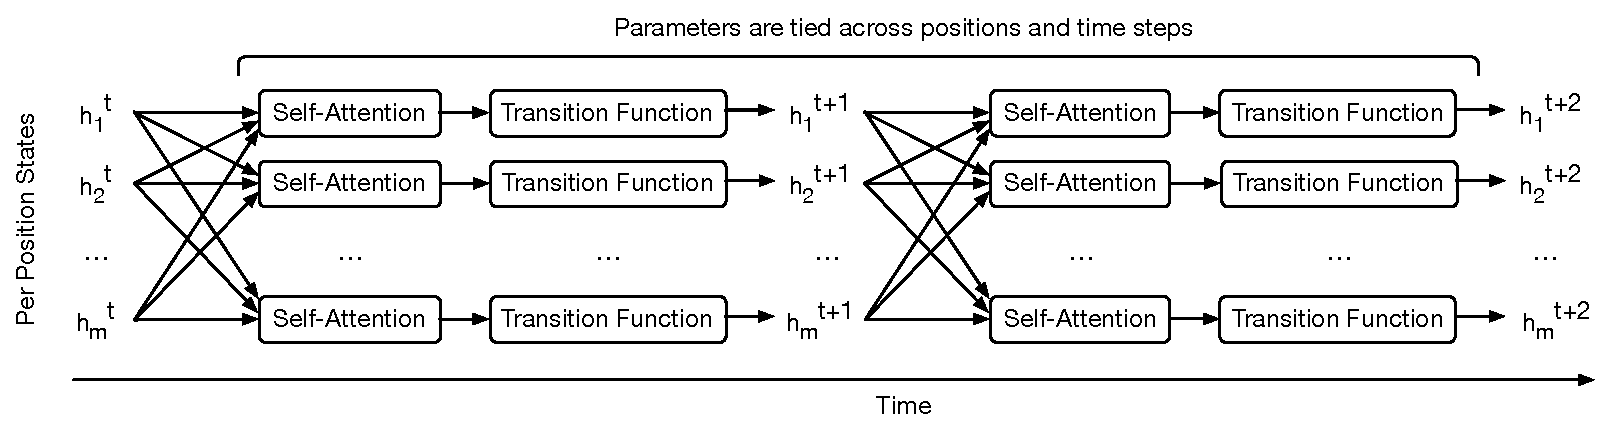
\includegraphics[width=\textwidth]{04-part-03/chapter-06/figs_and_tables/fig_universal-transformer-as-rnn.pdf}
 \caption{The Universal Transformer repeatedly refines a series of vector representations for each position of the sequence in parallel, by combining information from different positions using self-attention (see Eqn~\ref{MultiheadSelfAttention}) and applying a recurrent transition function (see Eqn~\ref{RecurrentTransition}) across all time steps $1 \leq t \leq T$. We show this process over two recurrent time-steps. Arrows denote dependencies between operations. Initially, $h^0$ is initialized with the embedding for each symbol in the sequence. $h^t_i$ represents the representation for input symbol $1 \leq i \leq m$ at recurrent time-step $t$. With dynamic halting, $T$ is dynamically determined for each position (Section~\ref{sec:dynamic-halting}).}
 \label{fig:rec-state}
\end{figure}


We introduce the \emph{Universal Transformer (UT)}, a parallel-in-time recurrent self-attentive sequence model which can be cast as a generalization of the Transformer model, yielding increased theoretical capabilities and improved results on a wide range of challenging sequence-to-sequence tasks. UTs combine the parallelizability and global receptive field of feed-forward sequence models like the Transformer with the recurrent inductive bias of RNNs, which seems to be better suited to a range of algorithmic and natural language understanding sequence-to-sequence problems. As the name implies, and in contrast to the standard Transformer, under certain assumptions UTs can be shown to be Turing-complete (or ``computationally universal'', as shown in Section~\ref{sec:related}).

In each recurrent step, the Universal Transformer iteratively refines its representations for all symbols in the sequence in parallel using a self-attention mechanism~\citep{decomposableAttnModel,lin2017structured}, followed by a transformation (shared across all positions and time-steps) consisting of a depth-wise separable convolution \citep{xception2016,slicenet} or a position-wise fully-connected layer (see Fig~\ref{fig:rec-state}). We also add a dynamic per-position halting mechanism \citep{graves2016adaptive}, allowing the model to choose the required number of refinement steps \emph{for each symbol} dynamically, and show for the first time that such a conditional computation mechanism can in fact improve accuracy on several smaller, structured algorithmic and linguistic inference tasks (although it marginally degraded results on MT). 

Our strong experimental results show that UTs outperform Transformers and LSTMs across a wide range of tasks. The added recurrence yields improved results in machine translation where UTs outperform the standard Transformer. In experiments on several algorithmic tasks and the bAbI language understanding task, UTs also consistently and significantly improve over LSTMs and the standard Transformer. Furthermore, on the challenging LAMBADA text understanding data set UTs with dynamic halting achieve a new state of the art.

\subsection{Detailed Research Questions}
We break down our main research question in this chapter into two concrete research questions:
\begin{resqbox}
\begin{enumerate}
\item[\textbf{\resqname{c6.1}}] \emph{\resqcontent{c6.1}}
\item[\textbf{\resqname{c6.2}}] \emph{\resqcontent{c6.2}}
\end{enumerate}
\end{resqbox}

In the following sections, we will address these research questions.

\section{The Universal Transformer }%: A Self-attentive Concurrent-Recurrent Sequence Model}
Here, in this section, we focus on the following research question:
\resq{c6.1}

The Universal Transformer (UT; see Fig.~\ref{fig:universal-transformer-complete}) is based on the popular encoder-decoder architecture commonly used in most neural sequence-to-sequence models \citep{sutskever14,cho2014learning,transformer}. Both the encoder and decoder of the UT operate by applying a recurrent neural network to the representations of each of the positions of the input and output sequence, respectively. However, in contrast to most applications of recurrent neural networks to sequential data, the UT does not recur over positions in the sequence, but over consecutive revisions of the vector representations of each position (i.e., over ``depth''). In other words, the UT is not computationally bound by the number of symbols in the sequence, but only by the number of revisions made to each symbol's representation.

In each recurrent time-step, the representation of every position is concurrently (in parallel) revised in two sub-steps: first, using a self-attention mechanism to exchange information across all positions in the sequence, thereby generating a vector representation for each position that is informed by the representations of all other positions at the previous time-step. Then, by applying a transition function (shared across position and time) to the outputs of the self-attention mechanism, independently at each position. As the recurrent transition function can be applied any number of times, this implies that UTs can have variable depth (number of per-symbol processing steps). Crucially, this is in contrast to most popular neural sequence models, including the Transformer~\citep{transformer} or deep RNNs, which have constant depth as a result of applying a \emph{fixed stack} of layers. We now describe the encoder and decoder in more detail.

\begin{figure}[t]
 \centering
 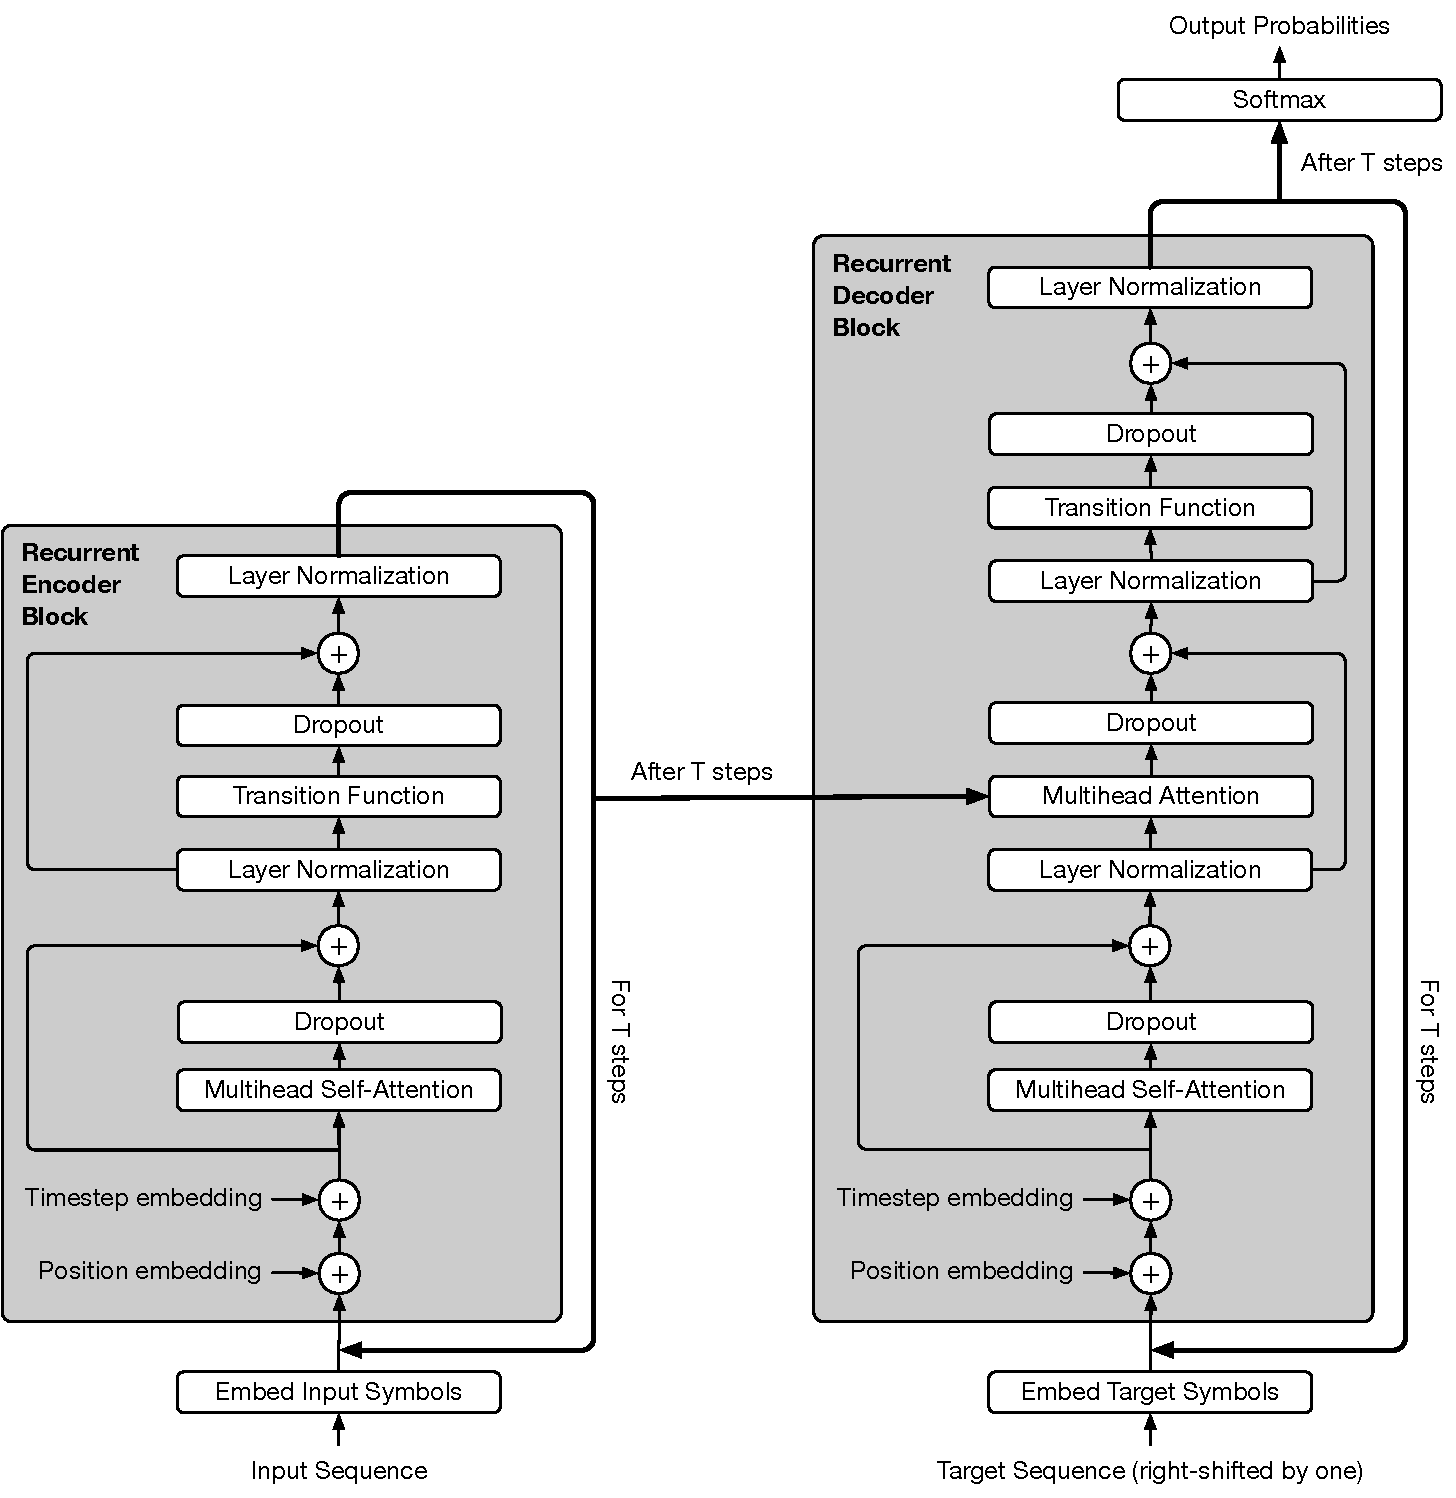
\includegraphics[width=0.9\textwidth]{04-part-03/chapter-06/figs_and_tables/fig_universal-transformer-complete.pdf}
 \caption{The recurrent blocks of the Universal Transformer encoder and decoder.}
 \label{fig:universal-transformer-complete}
\end{figure}

\textbf{\textsc{Encoder:}} Given an input sequence of length $m$, we start with a matrix whose rows are initialized as the $d$-dimensional embeddings of the symbols at each position of the sequence $H^0 \in \mathbb{R}^{m \times d}$. The UT then iteratively computes representations $H^t$ at step $t$ for all $m$ positions in parallel by applying the multi-headed dot-product self-attention mechanism from \cite{transformer}, followed by a recurrent transition function. We also add residual connections around each of these function blocks and apply dropout and layer normalization \citep{srivastava2014dropout, layernorm2016} (See Figure~\ref{fig:universal-transformer-complete} for the schema of the complete model.).

More specifically, we use the scaled dot-product attention which combines queries $Q$, keys $K$ and values $V$ as follows

\begin{equation}
   \textsc{Attention}(Q, K, V) = \textsc{softmax} \left( \frac{QK^T}{\sqrt{d}} \right) V,
\end{equation}

where $d$ is the number of columns of $Q$, $K$ and $V$. We use the multi-head version with $k$ heads, as introduced in \citep{transformer},

\begin{align}
    \label{MultiheadSelfAttention}
    \textsc{MultiHeadSelfAttention}(H^t) &= \textsc{Concat}(\mathrm{head_1}, ..., \mathrm{head_k})W^O\\
    \text{where}~\mathrm{head_i} &= \textsc{Attention}(H^t W^Q_i, H^t W^K_i, H^t W^V_i)
\end{align}

and we map the state $H^t$ to queries, keys and values with affine projections using learned parameter matrices $W^Q \in \mathbb{R}^{d \times d/k}$, $W^K \in \mathbb{R}^{d \times d/k}$, $W^V \in \mathbb{R}^{d \times d/k}$ and $W^O \in \mathbb{R}^{d \times d}$.

At step $t$, the UT then computes revised representations $H^t \in \mathbb{R}^{m \times d}$ for all $m$ input positions as follows

\begin{align}
    \label{RecurrentTransition}
    H^t &= \textsc{LayerNorm}(A^{t} + \textsc{Transition}(A^t) ) \\
    \mathrm{where}~A^t &= \textsc{LayerNorm}((H^{t-1} + P^{t}) + \textsc{MultiHeadSelfAttention}(H^{t-1} + P^{t})),
\end{align}
where \textsc{LayerNorm()} is defined in \cite{layernorm2016}, and \textsc{Transition()} and $P^t$ are discussed below.

Depending on the task, we use one of two different transition functions: either a separable convolution~\citep{xception2016} or a fully-connected neural network that consists of a single rectified-linear activation function between two affine transformations, applied position-wise, i.e., individually to each row of $A^t$.

$P^t \in \mathbb{R}^{m \times d}$ above are fixed, constant, two-dimensional (position, time) \emph{coordinate embeddings}, obtained by computing the sinusoidal position embedding vectors as defined in \citep{transformer} for the positions $1 \leq i \leq m$ and the time-step $1 \leq t \leq T$ separately for each vector-dimension $1 \leq j \leq d$, and summing:
\begin{align}
\label{eqn:coordinate-embeddings}
    P^t_{i, 2j} &= \sin(i / 10000^{2j / d}) + \sin(t / 10000^{2j / d}) \\
    P^t_{i, 2j+1} &= \cos(i / 10000^{2j / d}) + \cos(t / 10000^{2j / d}).
\end{align}

After $T$ steps (each updating all positions of the input sequence in parallel), the final output of the Universal Transformer encoder is a matrix of $d$-dimensional vector representations $H^T \in \mathbb{R}^{m \times d}$ for the $m$ symbols of the input sequence.

\textbf{\textsc{Decoder:}} The decoder shares the same basic recurrent structure of the encoder. However, after the self-attention function, the decoder additionally also attends to the final encoder representation $H^T$ of each position in the input sequence using the same multihead dot-product attention function from Equation \ref{MultiheadSelfAttention}, but with queries $Q$ obtained from projecting the decoder representations, and keys and values ($K$ and $V$) obtained from projecting the encoder representations (this process is akin to standard attention \citep{bahdanau2014neural}).

Like the Transformer model, the UT is autoregressive \citep{graves2013generating}. Trained using teacher-forcing, at generation time it produces its output one symbol at a time, with the decoder consuming the previously produced output positions. During training, the decoder input is the target output, shifted to the right by one position.
The decoder self-attention distributions are further masked so that the model can only attend to positions to the left of any predicted symbol. Finally, the per-symbol target distributions are obtained by applying an affine transformation $O \in \mathbb{R}^{d \times V}$ from the final decoder state to the output vocabulary size $V$, followed by a softmax which yields an $(m \times V)$-dimensional output matrix normalized over its rows:

\begin{equation}
 p\left(y_{pos} | y_{[1:pos - 1]}, H^T\right) = \textsc{softmax}(OH^T)\footnote{Note that $T$ here denotes time-step $T$ and not the transpose operation.}
\end{equation}

To generate from the model, the encoder is run once for the conditioning input sequence. Then the decoder is run repeatedly, consuming all already-generated symbols, while generating one additional distribution over the vocabulary for the symbol at the next output position per iteration. We then typically sample or select the highest probability symbol as the next symbol.


\subsection{Adaptive Computation by Dynamic Halting}
\label{sec:dynamic-halting}
\begin{figure}
 \centering
 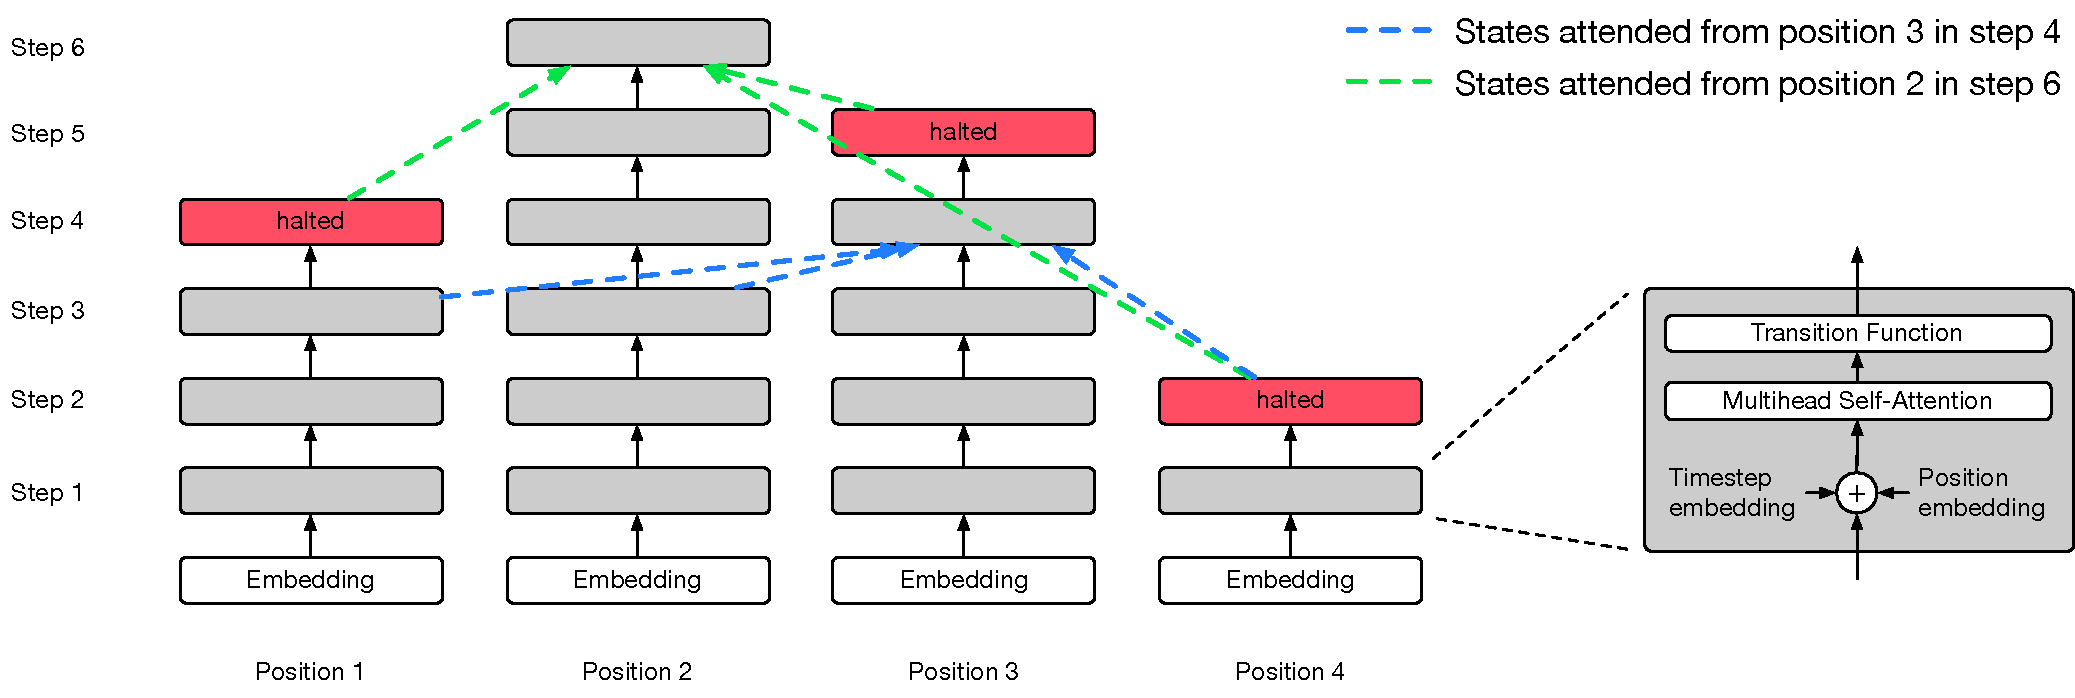
\includegraphics[width=1.0\textwidth]{04-part-03/chapter-06/figs_and_tables/fig_adaptive-universal-transformer.pdf}
 \caption{An unrolled visualization of Universal Transformer with dynamic halting. It illustrates different numbers of recurrent revisions per position (best viewed in colour).}
 \label{fig:adaptive_ut}
\end{figure}
In sequence processing systems, certain symbols (e.g., some words or phonemes) are usually more ambiguous than others. It is therefore reasonable to allocate more processing resources to these more ambiguous symbols. Adaptive Computation Time (ACT) \citep{graves2016adaptive} is a mechanism for dynamically modulating the number of computational steps needed to process each input symbol (called the ``ponder time'') in standard recurrent neural networks based on a scalar \emph{halting probability} predicted by the model at each step.

Inspired by the interpretation of Universal Transformers as applying self-attentive RNNs in parallel to all positions in the sequence, we also add a dynamic ACT halting mechanism to each position, i.e., to each per-symbol self-attentive RNN. Once the per-symbol recurrent block halts, its state is simply copied to the next step until all blocks halt, or we reach a maximum number of steps. The final output of the encoder is then the final layer of representations produced in this way. Figure~\ref{fig:adaptive_ut} illustrates a Universal Transformer encoder with $T$, number of revisions, dynamically determined for each position.


We implement the dynamic halting based on ACT~\citep{graves2016adaptive} as follows in TensorFlow. In each step of the UT with dynamic halting, we are given the halting probabilities, remainders, number of updates up to that point, and the previous state (all initialized as zeros), as well as a scalar threshold between 0 and 1 (a hyper-parameter). We then compute the new state for each position and calculate the new per-position halting probabilities based on the state for each position~\footnote{The current implementation of adaptive computation time does not allow for a fully ``end-to-end backpropable'' gradient of the proposed training loss. However, the discontinuity of the cost function might not imply that meaningful learning is not possible and in fact, the experiments in the original paper~\citep{graves2016adaptive} as well as here in Universal Transformer with adaptive halting suggest it works fine.}. The UT then decides to halt for some positions that crossed the threshold, and updates the state of other positions until the model halts for all positions or reaches a predefined maximum number of steps:
\input{04-part-03/chapter-06/figs_and_tables/alg_ut_with_act.tex}


\section{Universality and Relation to other Models}
\label{sec:related}
When running for a fixed number of steps, the Universal Transformer is equivalent to a multi-layer Transformer with tied parameters across all its layers. This is partly similar to the Recursive Transformer, which ties the weights of its self-attention layers across depth~\citep{gulcehre2018hyperbolic}\footnote{Note that in UT both the self-attention and transition weights are tied across layers.}. However, as the per-symbol recurrent transition functions can be applied any number of times, another and possibly more informative way of characterizing the UT is as a block of parallel RNNs (one for each symbol, with shared parameters) evolving per-symbol hidden states concurrently, generated at each step by attending to the sequence of hidden states at the previous step. In this way, it is related to architectures such as the Neural GPU \citep{neural_gpu} and the Neural Turing Machine \citep{ntm14}. UTs thereby retain the attractive computational efficiency of the original feed-forward Transformer model, but with the added recurrent inductive bias of RNNs. Furthermore, using a dynamic halting mechanism, UTs can choose the number of processing steps based on the input data. %interpolate between the feed-forward, fixed-depth Transformer and a gated, recurrent architecture running for a number of steps dependent on the input data. 

The connection between the Universal Transformer and other sequence models is apparent from the architecture: if we limited the recurrent steps to one, it would be a Transformer. But it is more interesting to consider the relationship between the Universal Transformer and RNNs and other networks where recurrence happens over the time dimension. Superficially these models may seem closely related since they are recurrent as well. But there is a crucial difference: time-recurrent models like RNNs cannot access memory in the recurrent steps. This makes them computationally more similar to automata, since the only memory available in the recurrent part is a fixed-size state vector. UTs, on the other hand, can attend to the whole previous layer, allowing it to access memory in the recurrent step. 

Given sufficient memory the Universal Transformer is computationally universal -- i.e., it belongs to the class of models that can be used to simulate any Turing machine, thereby addressing a shortcoming of the standard Transformer model. In addition to being theoretically appealing, our results show that this added expressivity also leads to improved accuracy on several challenging sequence modeling tasks. This closes the gap between practical sequence models competitive on large-scale tasks such as machine translation, and computationally universal models such as the Neural Turing Machine or the Neural GPU \citep{ntm14,neural_gpu}, which can be trained using gradient descent to perform algorithmic tasks.

To show this, we can reduce a Neural GPU to a Universal Transformer. Ignoring the decoder and parameterizing the self-attention module, i.e., self-attention with the residual connection, to be the identity function, we assume the transition function to be a convolution. If we now set the total number of recurrent steps $T$ to be equal to the input length, we obtain exactly a Neural GPU. Note that the last step is where the Universal Transformer crucially differs from the vanilla Transformer whose depth cannot scale dynamically with the size of the input. A similar relationship exists between the Universal Transformer and the Neural Turing Machine, whose single read/write operations per step can be expressed by the global, parallel representation revisions of the Universal Transformer. In contrast to these models, however, which only perform well on algorithmic tasks, the Universal Transformer also achieves competitive results on realistic natural language tasks such as LAMBADA and machine translation.

Another related model architecture is that of end-to-end Memory Networks \citep{sukhbaatar2015}. In contrast to end-to-end memory networks, however, the Universal Transformer uses memory corresponding to states aligned to individual positions of its inputs or outputs. Furthermore, the Universal Transformer follows the encoder-decoder configuration and achieves competitive performance in large-scale sequence-to-sequence tasks.


\subsection{On the Computational Power of UT vs Transformer}
\label{app:univerrality_example}

With respect to their computational power, the key difference between the Transformer and the Universal Transformer lies in the number of sequential steps of computation (i.e., in depth). While a standard Transformer executes a total number of operations that scales with the input size, the number of sequential operations is constant, independent of the input size and determined solely by the number of layers. Assuming finite precision, this property implies that the standard Transformer cannot be computationally universal. When choosing a number of steps as a function of the input length, however, the Universal Transformer does not suffer from this limitation. Note that this holds independently of whether or not adaptive computation time is employed but does assume a non-constant, even if possibly deterministic, number of steps. Varying the number of steps dynamically after training is enabled by sharing weights across sequential computation steps in the Universal Transformer.

\begin{figure}[t]
\centering
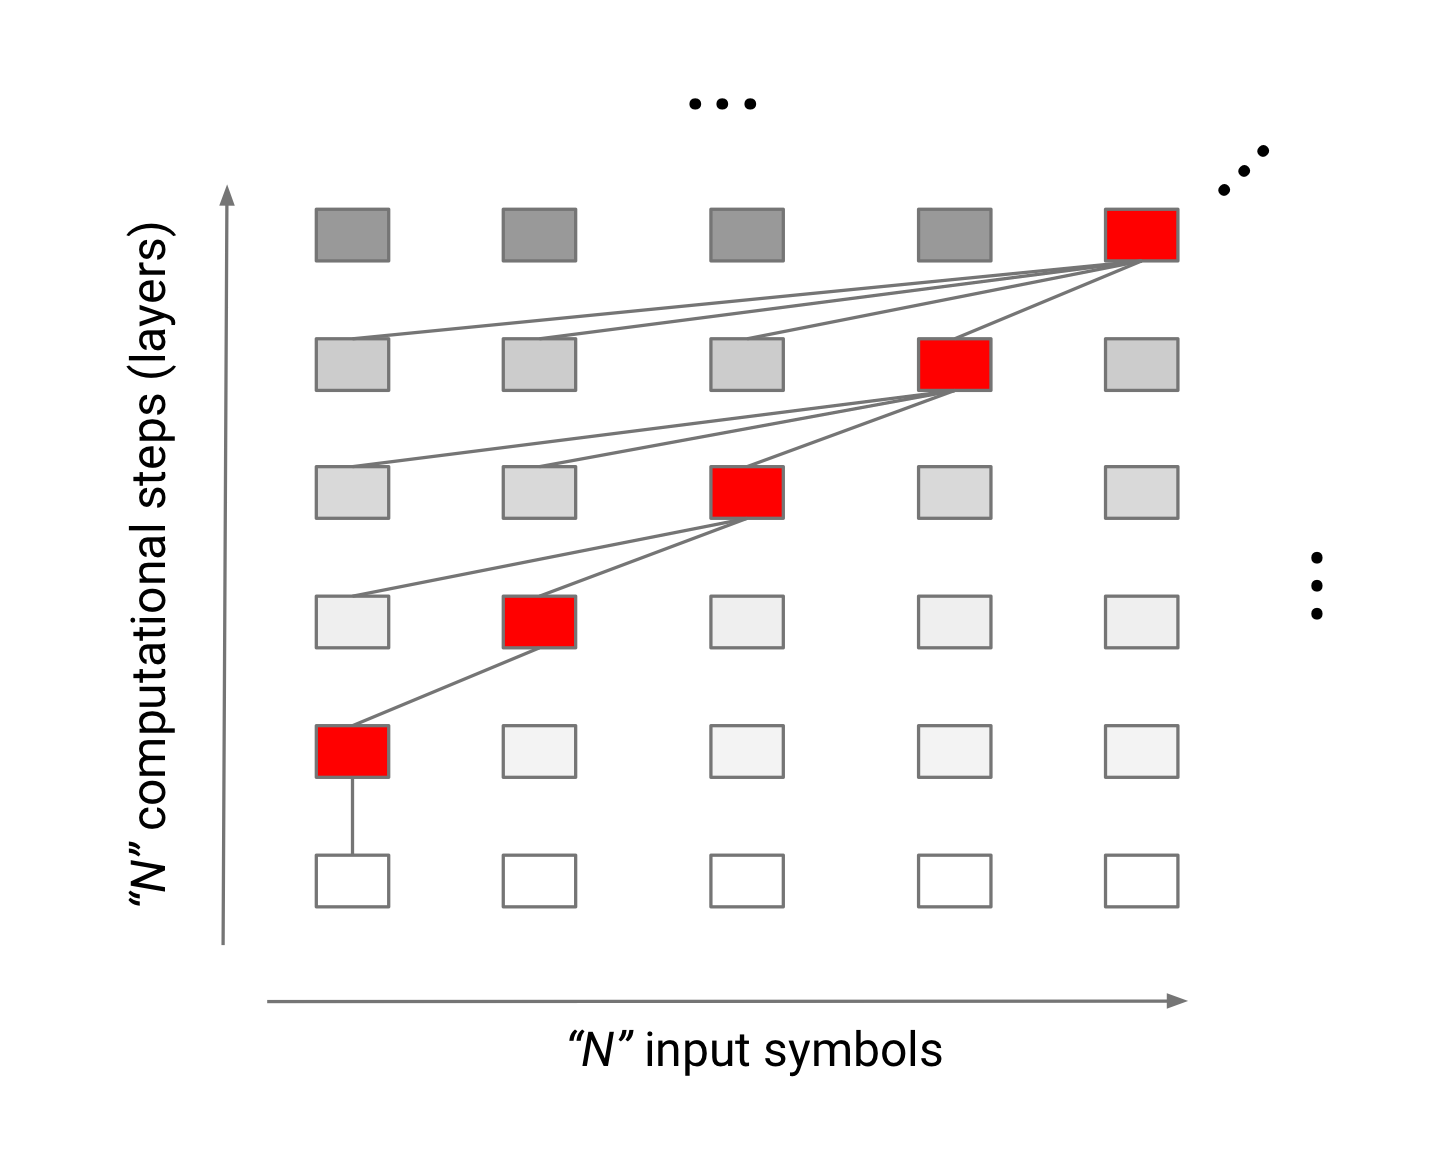
\includegraphics[width=0.6\textwidth, trim={0.1cm 0.5cm 0.1cm 1.2cm}, clip]{04-part-03/chapter-06/figs_and_tables/fig_universality_example.png}
\end{figure}

An intuitive example are functions whose execution requires the sequential processing of each input element. In this case, for any given choice of depth $T$, one can construct an input sequence of length $N>T$ that cannot be processed correctly by a standard Transformer. With an appropriate, input-length dependent choice of sequential steps, however, a Universal Transformer, RNNs or Neural GPUs can execute such a function.
\section{Universal Transformer for Sequence Modeling}
In this section, we address the following research question:
\resq{c6.2}
We evaluate Universal Transformers on a range of algorithmic and language understanding tasks and discuss the results. In the tasks that are chosen, we include some with limited number of training samples, or some with incomplete training set (lack of converge), but also tasks that do not suffer severely from imperfect supervision, to evaluate the performance of our model in both situations. 

\subsection{bAbI Question-Answering}
The bAbi question answering dataset~\citep{weston2015towards} consists of 20 different synthetic tasks\footnote{\url{https://research.fb.com/downloads/babi}}. The aim is that each task tests a unique aspect of language understanding and reasoning, including the ability of: reasoning from supporting facts in a story, answering true/false type questions, counting, understanding negation and indefinite knowledge, understanding coreferences, time reasoning, positional and size reasoning, path-finding, and understanding motivations (to see examples for each of these tasks, please refer to Table 1 in \citep{weston2015towards}).

There are two versions of the dataset, one with 1k training samples and the other with 10k samples. It is important for a model to be data-efficient to achieve good results using only the 1k training samples. Moreover, the original idea is that a single model should be evaluated across all the tasks (not tuning per task), which is the \emph{train joint} setup in Tables~\ref{tab:babi-results} and ~\ref{tbl:babi_details}.

Solving all the bAbI tasks by training a model on the 1k training dataset is pretty challenging as some of the tasks are rather complex and with only 1k samples for each task, its hard for most of models to generalize well. So data efficiency should be a key property to be considered here. 
We tried a standard Transformer and observed that it does not achieve good results on bAbI tasks\footnote{We experimented with different hyper-parameters and different network sizes, but it always overfits.}. However, we have designed a model based on the Universal Transformer which achieves state-of-the-art results bAbI task. 
This is mainly due to recurrent inductive bias in the Universal Transformer as well as the fact that sharing parameters across depth decreases the number of parameters which helps the model generalize better.

To encode the input, similar to~\cite{henaff2016tracking}, we first encode each fact in the story by applying a learned multiplicative positional mask to each word's embedding, and summing up all embeddings.
We embed the question in the same way, and then feed the (Universal) Transformer with these embeddings of the facts and questions. 

As originally proposed, models can either be trained on each task separately (``train single'') or jointly on all tasks (``train joint''). Table~\ref{tab:babi-results} summarizes our results. We conducted 10 runs with different initializations and picked the best model based on performance on the validation set, similar to previous work. Both the UT and UT with dynamic halting achieve state-of-the-art results on all tasks in terms of average error and number of failed tasks\footnote{Defined as $> 5\%$ error.}, in both the 10K and 1K training regime. Tables~\ref{tbl:babi_details} presents the results of best and average results of 10 runs breakdown by task.

\input{04-part-03/chapter-06/figs_and_tables/table_babi_results.tex}
\input{04-part-03/chapter-06/figs_and_tables/table_babi_detailed_results.tex}


To understand the working of the model better, we analyzed both the attention distributions and the average ACT ponder times for this task. First, we observe that the attention distributions start out very uniform, but get progressively sharper in later steps around the correct supporting facts that are required to answer each question, which is indeed very similar to how humans would solve the task. 
%
Second, with dynamic halting we observe that the average ponder time (i.e., depth of the per-symbol recurrent processing chain) over all positions in all samples in the test data for tasks requiring three supporting facts is higher ($3.8 \rpm 2.2$) than for tasks requiring only two ($3.1 \rpm 1.1$), which is in turn higher than for tasks requiring only one supporting fact ($2.3 \rpm 0.8$). This indicates that the model adjusts the number of processing steps with the number of supporting facts required to answer the questions. 

\begin{figure}[t]
 \centering
 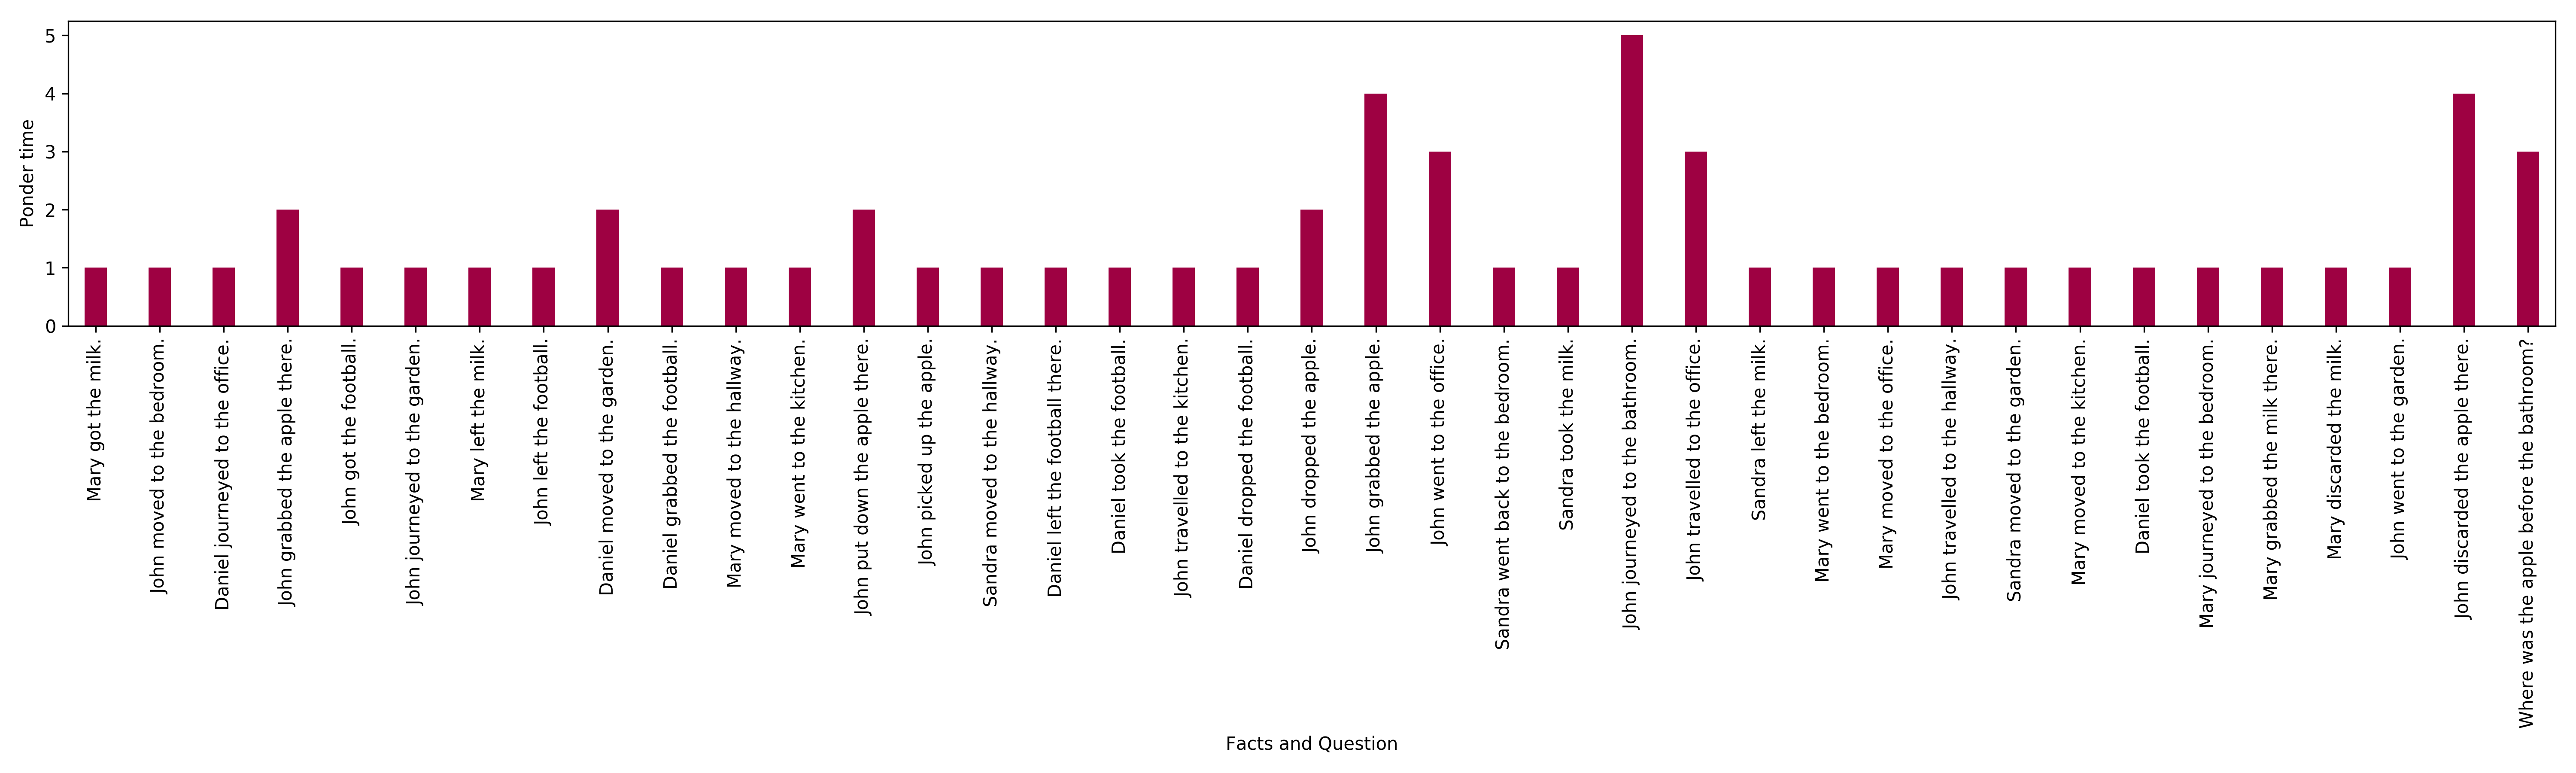
\includegraphics[width=\textwidth]{04-part-03/chapter-06/figs_and_tables/fig_task3_example_ponder.png}
 \caption{Ponder time of UT with dynamic halting for encoding facts in a story and question in a bAbI task requiring three supporting facts.}
 \label{fig:act_ponder}
\end{figure}
Finally, we observe that the histogram of ponder times at different positions is more uniform in tasks requiring only one supporting fact compared to two and three, and likewise for tasks requiring two compared to three.  Especially for tasks requiring three supporting facts, many positions halt at step 1 or 2 already and only a few get transformed for more steps (see, for example, Figure~\ref{fig:act_ponder}). This is particularly interesting as the length of stories is indeed much higher in this setting, with more irrelevant facts which the model seems to successfully learn to ignore in this way.

Similar to dynamic memory networks~\citep{kumar2016ask}, there is an iterative attention process in UTs that allows the model to condition its attention over memory on the result of previous iterations. 
%

\input{04-part-03/chapter-06/figs_and_tables/fig_babi_attention_examples.tex}

Figures~\ref{fig:ex1}, \ref{fig:ex2}, \ref{fig:ex3}, and \ref{fig:ex4} present visualizations of the attention distributions on bAbI tasks for some examples from Task 1, 2, and 3. The visualization of attention weights is over different time steps based on different heads over all the facts in the story and a question. Different color bars on the left side indicate attention weights based on different heads (4 heads in total).

The above examples illustrate that there is a notion of temporal states in UT, where the model updates its states (memory) in each step based on the output of previous steps, and this chain of updates can also be viewed as steps in a multi-hop reasoning process.

\subsection{Algorithmic Tasks}
The generic neural network architectures cannot generalize well in algorithmic and numerical tasks requiring arithmetic operations such as addition, multiplication etc., even when they may successfully fit any given training data in such tasks, and sometimes they cannot even achieve that~\citep{trask2018neural}. This can be even harder when the distribution of samples' length is different in train and test set.

We trained UTs on three algorithmic tasks, namely Copy, Reverse, and (integer) Addition, all on strings composed of decimal symbols (`0'-`9'). In all the experiments, we train the models on sequences with maximum length of 40 and evaluated on sequences with maximum length of 400~\citep{neural_gpu} to assess the ability of the models on \emph{length generalization}. In fact, the limitation in training data in this task is the lack of coverage over all possible samples (all possible length), not the number of training samples.

As an additional inductive bias for UTs on these tasks, when calculating the positional embedding, we use positions starting with randomized offsets per sample. This way, we further encourage the model to learn position-relative transformations, which improves length generalization.
Results are shown in Table~\ref{tab:algorithmic}. Both UT and UT with randomized position offset outperform LSTM and vanilla Transformer by a wide margin on all three tasks. 
The Neural GPU reports perfect results on this task~\citep{neural_gpu}, however, we note that this result required a special curriculum-based training protocol which was not used for other models.

\input{04-part-03/chapter-06/figs_and_tables/table_alg_results.tex}

\subsection{Learning to Execute (LTE)}
As another class of sequence-to-sequence learning problems, we also evaluate UTs on Learning to Execute (LTE) tasks. 
LTE is a set of tasks indicating the ability of a model to learn to execute computer programs and was proposed by~\citet{ZS14}. These tasks include two subsets: 1) program evaluation tasks (program, control, and addition) that are designed to assess the ability of models for understanding numerical operations, if-statements, variable assignments, the compositionality of operations, and more, as well as 2) memorization tasks (copy, double, and reverse). 

The difficulty of the program evaluation tasks is parameterized by their \textit{length} and \textit{nesting}. The
length parameter is the number of digits in the integers that appear in the programs (so the integers are chosen uniformly from [1, \emph{length}]), and the nesting parameter is the number of times we are allowed to combine the operations with each
other. Higher values of nesting yield programs with deeper parse trees.
For instance, here is a program that is generated with length = 4 and
nesting = 3. 
\begin{table}[h!]
\fontsize{8}{8}\fontfamily{pcr}\selectfont
\begin{tabular}{l l}
\textbf{Input}: & \\
& j=8584 \\
& {\color{blue}{for}} x {\color{blue}{in}} range(8): \\
& ~~j+=920 \\
& b=(1500+j) \\
& {\color{blue}{print}}((b+7567)) \\
\textbf{Target}: & \\
& 25011
\end{tabular}
\end{table}

\input{04-part-03/chapter-06/figs_and_tables/table_lte_results.tex}

We use the mix-strategy discussed in~\citep{ZS14} to generate the datasets. Unlike~\citep{ZS14}, we do not use any curriculum learning strategy during training and we make no use of target sequences at test time. Tables~\ref{tab:lte-mem} and \ref{tab:lte-prog} present the performance of an LSTM model, Transformer, and Universal Transformer on the program evaluation and memorization tasks, respectively. UT achieves perfect scores in all the memorization tasks and also outperforms both LSTMs and Transformers in all program evaluation tasks by a wide margin. 


\subsection{Subject-Verb Agreement}
Next, we consider the task of predicting number-agreement between subjects and verbs in English sentences~\citep{linzen2016assessing}. Succeeding in this task is a strong indicator that a model can learn to approximate syntactic structure and therefore it was proposed by~\citet{linzen2016assessing} as a proxy for assessing the ability of different models to capture hierarchical structure in natural language. 

Two experimental setups were proposed by ~\citet{linzen2016assessing} for training a model on this task: 1) training with a language modeling objective, i.e., next word prediction, and 2) as binary classification, i.e., predicting the number of the verb given the sentence. 
We follow the experimental protocol of ~\citet{linzen2016assessing} for solving the task using a language modeling training setup, i.e., a next word prediction objective, followed by calculating the ranking accuracy of the target verb at test time. 

In this task, in order to have different levels of difficulty, ``agreement attractors'' are used, i.e., one or more intervening nouns with the opposite number from the subject with the goal of confusing the model. In this case, the model needs to correctly identify the head of the syntactic subject that corresponds to a given verb and ignore the intervening attractors in order to predict the correct form of that verb.
Here are some examples for this task in which subjects and the corresponding verbs are in boldface and agreement attractors are underlined:
\begin{table}[h!]
\fontsize{9}{10}\fontfamily{pcr}\selectfont
\begin{tabular}{l l}
\textbf{No attractor:} & The \textbf{boy} \textbf{smiles}. \\
\textbf{One attractor:}  &  The \textbf{number} of \underline{men} \textbf{is} not clear. \\
\textbf{Two attractors:}  &  The \textbf{ratio} of \underline{men} to \underline{women} \textbf{is} not clear. \\
\textbf{Three attractors:} &  The \textbf{ratio} of \underline{men} to \underline{women} and \underline{children} \textbf{is} not clear. 
\end{tabular}
\end{table}

\input{04-part-03/chapter-06/figs_and_tables/table_sva_results.tex}
Our results are summarized in Table~\ref{tab:sva}. The best LSTM with attention from the literature achieves 99.18\% on this task~\citep{yogatama2018memory}, outperforming a vanilla Transformer~\citep{tran18}. UTs significantly outperform standard Transformers, and achieve an \emph{average} result comparable to the current state of the art (99.2\%). However, we see that UTs (and particularly with dynamic halting) perform progressively better than all other models as the number of attractors increases (see the last row, $\Delta$).
The recurrent inductive bias, i.e., the fact that we can repeat the computations in depth, helps the Universal Transformer to capture the hierarchical relations and better model the structure of the data.

\subsection{LAMBADA Language Modeling}
The LAMBADA task~\citep{paperno2016lambada} is a language modeling task consisting of predicting a missing target word given a broader context of 4-5 preceding sentences. The dataset was specifically designed so that humans are able to accurately predict the target word when shown the full context, but not when only shown the target sentence in which it appears. It, therefore, goes beyond language modeling, and tests the ability of a model to incorporate broader discourse and longer term context when predicting the target word\footnote{\url{http://clic.cimec.unitn.it/lambada/appendix_onefile.pdf}}.
Here is a sample from the dataset:

\begin{table}[h!]
\fontsize{8}{10}\fontfamily{pcr}\selectfont
\begin{tabular}{l l}
\textbf{Context}: & \\
& ``Yes, I thought I was going to lose the baby.'' \\
&  ``I was scared too,'' he stated, sincerity flooding his eyes. \\ 
&  ``You were?'' ``Yes, of course. Why do you even ask?''  \\
&  ``This baby wasn't exactly planned for.''
\\
\textbf{Target sentence}: & \\
& ``Do you honestly think that I would want you to have a \_\_\_\_\_\_\_\_?'' 
\\
\textbf{Target word}:  & \\  
& miscarriage
\end{tabular}
\end{table}

The LAMBADA task consists in predicting the target word given the whole passage (i.e., the context plus the target sentence). A ``control set''  is also provided which was constructed by randomly sampling passages of the same shape and size as the ones used to build LAMBADA, but without filtering them in any way. The control set is used to evaluate the models at standard language modeling before testing on the LAMBADA task, and therefore to ensure that low performance on the latter cannot be attributed simply to poor language modeling.

The task is evaluated in two settings: as \emph{language modeling} (the standard setup) and as \emph{reading comprehension}. In the former (more challenging) case, a model is simply trained for the next-word prediction on the training data, and evaluated on the target words at test time (i.e., the model is trained to predict all words, not specifically challenging target words).  In the latter setting, introduced by Chu et al.~\cite{chu2017broad}, the target sentence (minus the last word) is used as the query for selecting the target word from the context sentences. Note that the target word appears in the context 81\% of the time, making this setup much simpler. However, the task is impossible in the remaining 19\% of the cases.

\input{04-part-03/chapter-06/figs_and_tables/table_lambada_results.tex}

The results are shown in Table~\ref{tab:lambada}. Universal Transformer achieves state-of-the-art results in both the language modeling and reading comprehension setup, outperforming both LSTMs and vanilla Transformers. Note that achieving good results on the control set only shows a model's strength in standard language modeling.

Our best fixed UT results used 6 steps. However, the average number of steps that the best UT with dynamic halting took on the test data over all positions and samples was $8.2 \rpm 2.1$. In order to see if the dynamic model did better simply because it took more steps, we trained two fixed UT models with 8 and 9 steps respectively (see last two rows). Interestingly, these two models achieve better results compared to the model with 6 steps, but \emph{do not outperform the UT with dynamic halting}. This leads us to believe that dynamic halting may act as a useful regularizer for the model via incentivizing smaller numbers of steps for some of the input symbols, while allowing more computation for others.

\subsection{Machine Translation}
We trained a UT on the WMT 2014 English-German translation task using the same setup as reported in \citep{transformer} in order to evaluate its performance on a large-scale sequence-to-sequence task. Results are summarized in Table~\ref{tab:wmt}. The UT with a fully-connected recurrent transition function (instead of separable convolution) and without ACT improves by 0.9 BLEU over a Transformer and 0.5 BLEU over a Weighted Transformer with approximately the same number of parameters \citep{ahmed2017weighted}.

\input{04-part-03/chapter-06/figs_and_tables/table_mt_results.tex}

\subsection{Open-Domain Question Answering}
Open-domain question answering aims to satisfy users who are looking for a direct answer to a complex information need. 
This requires querying large open-domain knowledge sources like the Web. 
Inferring the answer to a question given multiple documents that potentially contain the answer, is at the heart of the open-domain question answering task. 
Most open-domain question answering systems described in the literature first retrieve relevant documents or passages, select one or a few of them as the context, and then feed the question and the context to a reading comprehension system to extract the answer~\citep{buck2017ask, chen2017reading, seo2016bidirectional, dhingra2016gated}. 
However, the information needed to answer complex questions is not always contained in a single, directly relevant document that is ranked high. In many cases, there is a need to read multiple documents, combine them, and reason over the facts from these documents to be able to give the correct answer to the question.

For example, in Figure~\ref{fig:example}, in order to infer the correct answer to the question: ``\texttt{Who is the Spanish artist, sculptor and draughtsman famous for co-founding the Cubist movement?}'' given the top-ranked document, a reading comprehension system most likely will extract ``\texttt{Georges Braque}'' as the answer, which is not the correct answer. 
In this example, in order to infer the correct answer, one has to go down the ranked list, gather and encode facts, even those that are not immediately relevant to the question, like ``\emph{Malaga is a city in Spain},'' which can be inferred from a document at rank 66, and then in a multi-step reasoning process, infer some new facts, including ``\emph{Picasso was a Spanish artist}'' given documents at ranks~12 and~66, and ``\emph{Picasso, who was a Spanish artist, co-founded the Cubist}'' given the previously inferred fact and the document ranked third. 

\begin{figure}[!t]
 \centering
 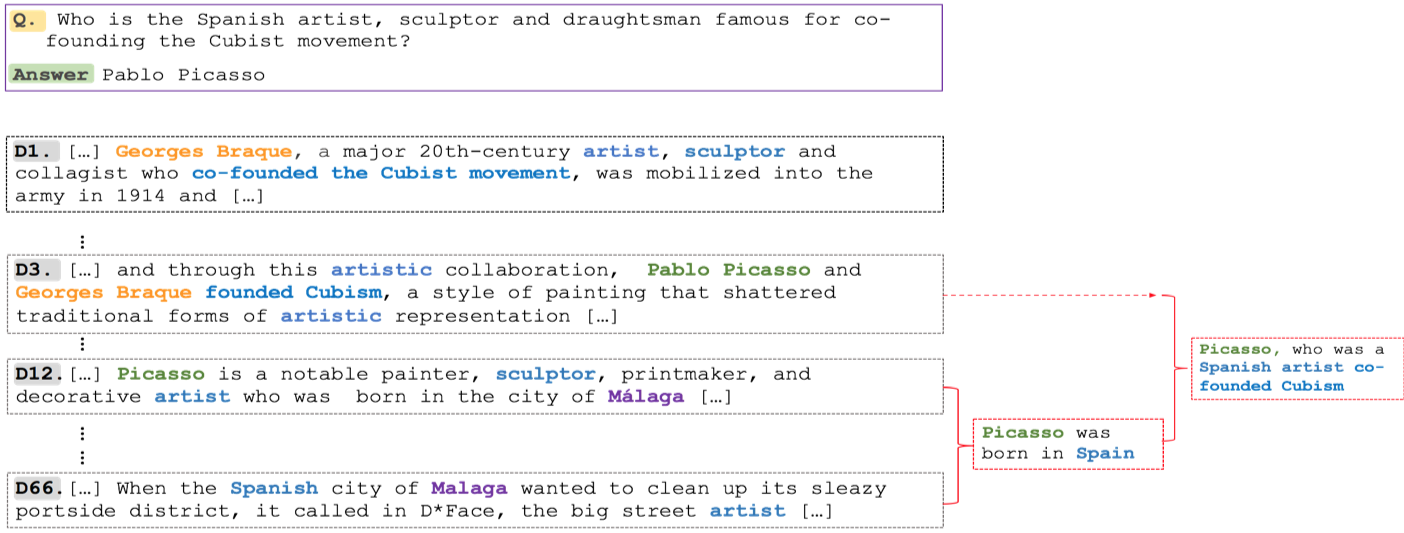
\includegraphics[width=\textwidth]{04-part-03/chapter-06/figs_and_tables/fig_od_example.png}
%  \vspace{1pt}
 \caption{Example complex question answering that requires that information from multiple documents be combined and some amount of reasoning over the information extracted from those documents. (Best viewed in color.)}
 \label{fig:example}
\end{figure}

In this example, and in general in many cases in open-domain question answering, a piece of information in a low-ranked document that is not immediately relevant to the question, may be useful to fill in the blanks and complete information extracted from the top relevant documents and eventually support inferring the correct answer.
However, most open-domain question answering methods focus on only one or a few candidate documents by filtering out the less relevant documents to avoid dealing with noisy information and operate over the selected set of documents to extract the answer~\citep{wang2017r, wang2017evidence,lin2018denoising}. 

We propose a new architecture, called \tracrnet (pronounced \emph{Tracker Net}, that combines Transformer and  Universal Transformer to improve open-domain question answering by explicitly operating on a larger set of candidate documents during the whole question answering process and learning how to aggregate and reason over information from these documents in an effective way while trying not to be distracted by noisy documents. 
% 
Given the candidate documents and the question, to generate the answer, \tracrnet first \underline{\textbf{Tra}}nsforms them into vectors by applying a stack of  Transformer blocks with self-attention over words in each document in a layer called \emph{Input Encoding}. 
Then, it updates the learned representations from the first stage by \underline{\textbf{C}}ombining and enriching them through a multihop \underline{\textbf{R}}easoning process by applying multiple steps of the Universal Transformer in a layer called \emph{Multihop Reasoning}.  

% paragraph might be too verbose
Returning to the example in Figure~\ref{fig:example}, after learning representations for each top-ranked document and the question, \tracrnet updates them by applying multiple steps of the Universal Transformer. 
Given the self-attention mechanism and inductive bias of the Universal Transformer, in the first step, \tracrnet can update the representation of document D\#12 by attending to D\#66 (as they are related by both mentioning Malaga) and augment the information in D\#12 with the fact that ``Malaga is city in Spain,'' so the updated vector of D\#12 has the fact that ``Picasso is a Spanish artist'' encoded in itself. 
Then, in the next step of reasoning, \tracrnet can update the representation of D\#3 by attending over the vector representing D\#12 estimated in the previous step, and enrich the information in D\#3 with the fact that ``Picasso is a Spanish artist,'' and the updated vector of D\#3 has the fact that ``Picasso, who was a Spanish artist co-founded Cubism'' encoded in it. 
After that, during answer generation, the decoder can attend to the final vector representing D\#3 and give the correct answer.

% why \tracrnet rocks:
% 1. fast
\tracrnet has a number of desirable features.
%
First, all the building blocks of \tracrnet are based on self-attentive feed-forward neural networks, hence per-symbol hidden state transformations are fully parallelizable, which leads to an enormous speedup during training and a super fast input encoding during inference time compared to RNN based models. 
% 3. It can reason
Second, while there is no recurrence in time in our model, the recurrence in depth in the Universal Transformer used in the \emph{Multihop Reasoning} layer, adds the inductive bias to the model that is needed to go beyond understanding each document separately and combine their information in multiple steps.
% 2. global receptive field -> long docs, a large set of docs
Third, \tracrnet has the global receptive field of the Transformer based models~\citep{vaswani2017attention,Dehghani:ICLR:2019}, which helps it to better encode a long document during \emph{Input Encoding} as well as perform better inference over a rather large set of documents during \emph{Multihop Reasoning}.
% 4. robustness against noise
And fourth, the hierarchical usage of a self-attention mechanism, first over words and then over documents, helps \tracrnet to control its attention both at word and document levels, making it less fragile to noisy input, which is of key importance while encoding many documents.
%
All these properties of \tracrnet come together and lead to an effective and efficient architecture for open-domain question answering. 

We employ \tracrnet on two public open-domain question answering datasets, SearchQA and Quasar-T, and achieve results that meet or exceed the state-of-the-art. 

\subsubsection{\tracrnet} % : Transform, Combine, and Reason}
\label{sec:tra}
In the setup we consider here, the model is given a question $q$ and a set of $n$ relevant documents $C_q=\{D^q_1, D^q_2, \ldots D^q_n\}$ retrieved from the web using a search engine as the input, and the goal is to ``generate'' the answer $a_q$ to the question $q$ based on the supporting document(s) in the set $C_q$.

This is different from the standard Reading Comprehension (RC) tasks~\cite{hermann2015teaching,xiong2016dynamic}. 
First of all, in RC a single document (passage) is given, from which the answer should be extracted. 
Secondly, in RC, a strong supervision on the positions of the answer spans is available during training.
We also assume that the utilized information or techniques to retrieve relevant documents are not available to the model, therefore there is no leverage for getting better-supporting documents.

\begin{figure}[!t]
 \centering
 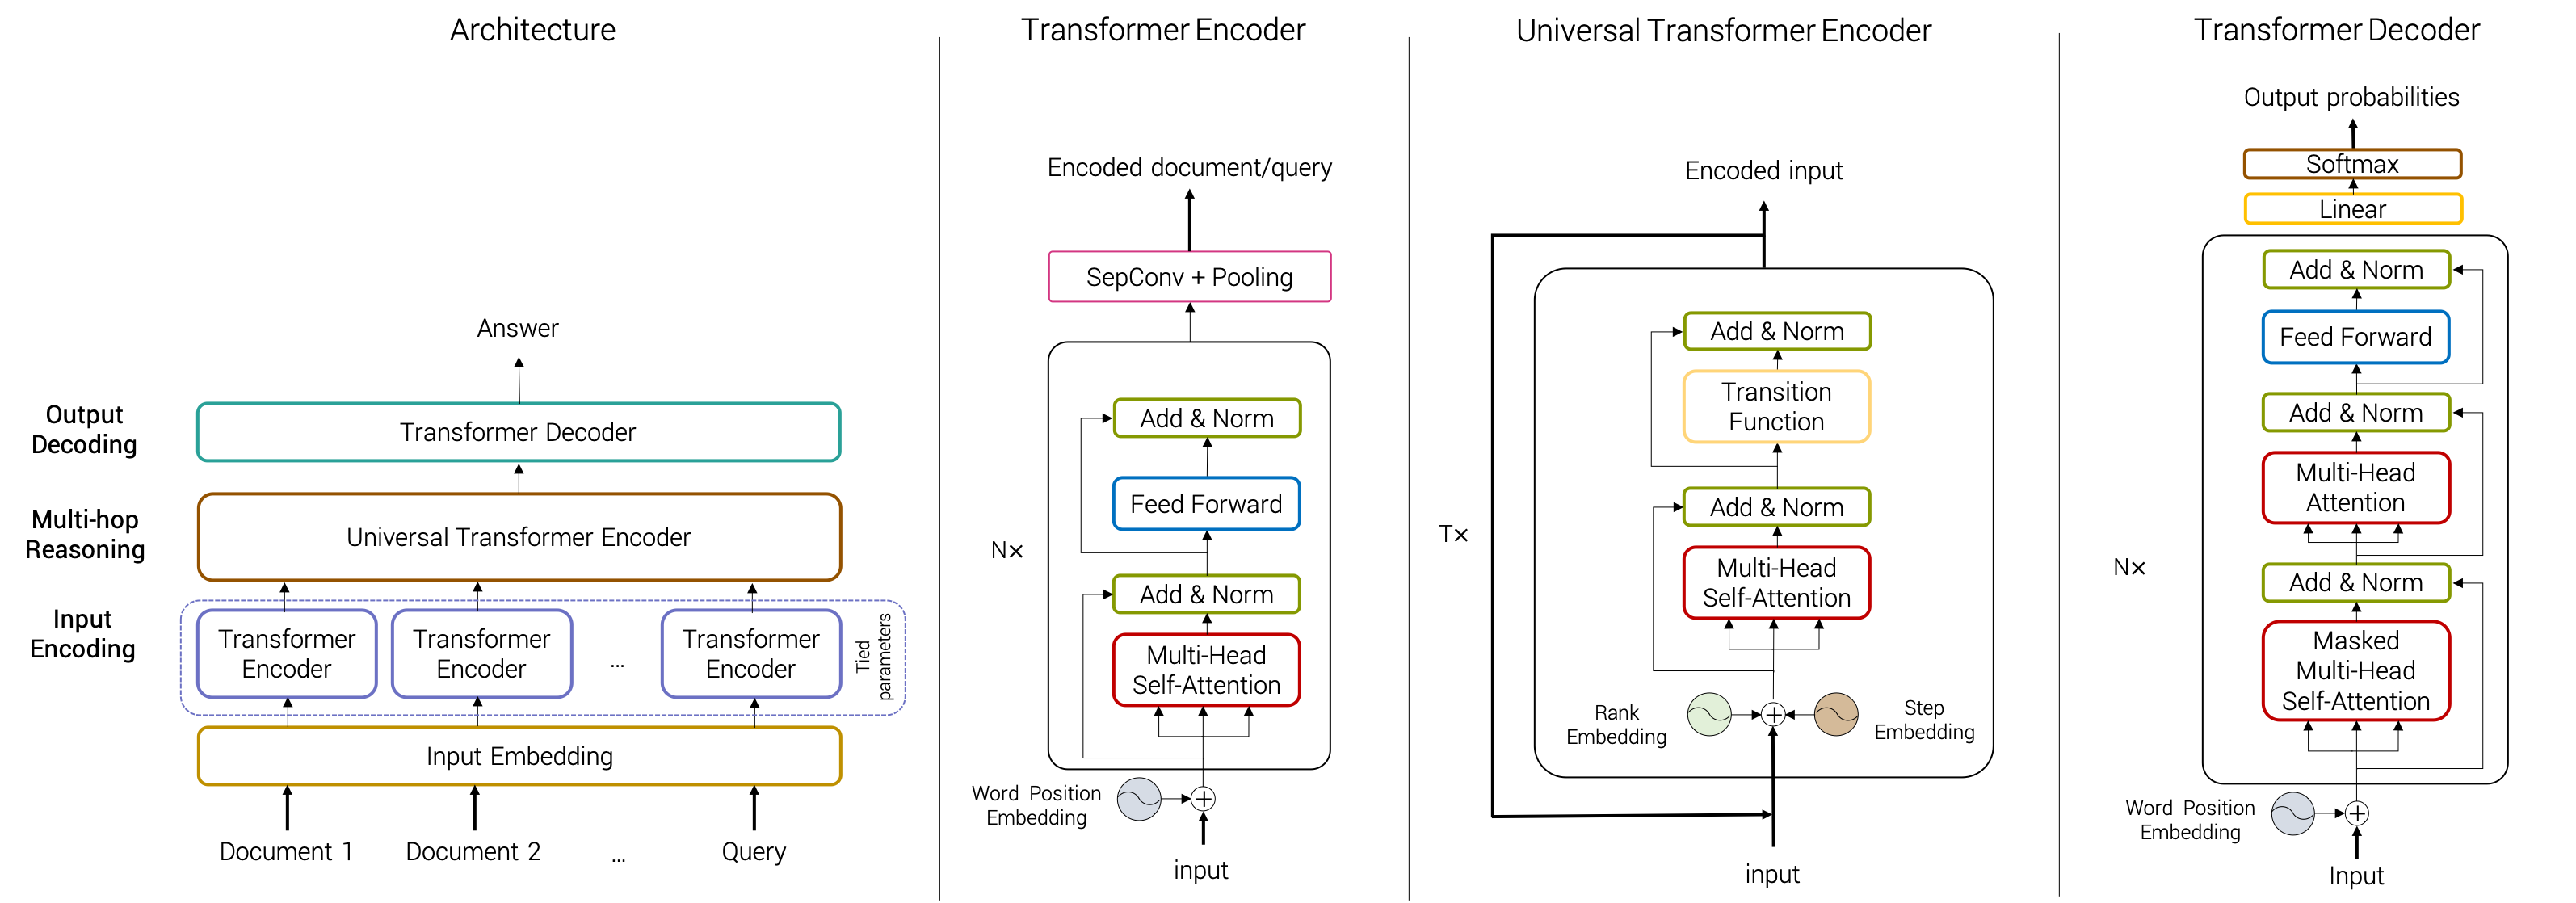
\includegraphics[width=\textwidth]{04-part-03/chapter-06/figs_and_tables/fig_tracrnet.png}
 \caption{An overview of the \tracrnet architecture.}
 \label{fig:model_tracrnet}
\end{figure}

\tracrnet is based on the encoder-decoder architecture, where we have a hierarchy of transformer-based models in the encoder, where the model can attend first over words and then over documents~\citep{Dehghani2017:CIKM}. At the bottom, in the \emph{Input Encoding} layer, we encode each document in $C_q$ as well as the question with transformer blocks with tied parameters that are fed by word-level embeddings. 
Then, we feed the encoded documents and the question from this layer to the \emph{Multihop Reasoning} layer which is, in fact, a universal transformer block where representations of all documents and the question get iteratively updated using multiple steps of self-attention.
Then, we use a stack of transformer decoder blocks as the \emph{Output Decoder} layer to generate the answer. 
%
The general schema of \tracrnet is depicted in Figure~\ref{fig:model_tracrnet}. 
Below, we explain the details of each of these layers in the model.

\mypar{Input encoding} 
The Input Encoding layer is in charge of encoding each of the documents and the question to single vectors given their words' embeddings. For this layer, we used a stack of $N$ Transformer Encoder blocks that is followed by a depth-wise separable convolution~\citep{kaiser2017depthwise,chollet2017xception} and then a pooling function to get a single vector representation for the whole document or the question  (see the \texttt{Transformer Encoder} in Figure~\ref{fig:model_tracrnet}). 
Depth-wise separable convolution is defined by a convolution on each of the feature channels separately, followed by a point-wise convolution that is applied to project them to a feature vector with the desirable depth (see \citep{chollet2017xception} for more details).

\mypar{Multihop reasoning} 
Multihop Reasoning is the layer in which the Universal Transformer is employed to combine evidence from all documents with respect to the question within a multi-step process with the capacity of multihop reasoning.
%
In \tracrnet, the input of the Universal Transformer Encoder is the set of vectors each representing a document in $C_q$ or the question, that are computed by the \emph{Input Encoding} layer  (see  the \texttt{Universal Transformer Encoder} in Figure~\ref{fig:model_tracrnet}). 

In each step of the Universal Transformer, given $H_{t} \in \mathbb{R}^{(|C_q|+1) \times d}$ and the dimension $d$ of the input vectors, we add two embeddings to $H^{t}$: a \emph{Rank Embedding} that encodes the rank of documents given by the retrieval system, also used to distinguish the question from documents (similar to the positional embedding in token level inputs) and the \emph{Step Embedding}. We use Equation\ref{eqn:coordinate-embeddings} to calculate these embeddings.
In our experiments, we use depthwise separable convolution~\cite{chollet2017xception} as the Transition($\cdot$) function.

In the multihop reasoning layer, the representations of all the documents and question learned from the previous layer get updated during $T$ steps of iterating over the Universal Transformer Encode block. 
Self-attention in this layer allows the model to understand each of the documents based on the information in all the documents as well as the question.
In addition, the depth-wise recurrency in the Universal Transformer establishes connections among documents at each step and lays the ground for performing multihop reasoning to solve cases similar to what we have shown in Example~\ref{fig:example}.

\mypar{Output decoder} 
After $T$ steps of refining the representations of documents and the question in the Universal Transformer Encoder, the final output is a matrix of $d$-dimensional vector representations $H \in \mathbb{R}^{(|C_q|+1) \times d}$ for all the documents in $C_q$ and the question $q$.

Given this, we use a stack of $N$ Transformer Decoder blocks (see  the \texttt{Transformer Decoder} in Figure~\ref{fig:model_tracrnet}) to decode the answer.
To generate answers from the model at inference time, we run the model autoregresively~\citep{graves2013generating}, where the model consumes the previously generated symbols at each time step in order to generate the distribution over the vocabulary for the next symbol. From this distribution, we select the symbol with the highest probability as the next symbol.   


\subsubsection{Datasets}
We have conducted experiments on two publicly available open-domain question answering datasets: SearchQA~\citep{dunn2017searchqa} and Quasar-T~\citep{dhingra2017quasar}. 
In both of these datasets, candidate documents (passages) for each question have already been retrieved using a search engine and we do not add any extra documents to these result sets. 
On both datasets, human performance is evaluated in a setup where the human subjects try to find the answers to the given question from the same documents retrieved by the IR model.

\mypar{SearchQA}
SearchQA\footnote{\url{https://github.com/nyu-dl/SearchQA}} is a dataset of 140k question-answer pairs crawled from J!\ Archive, and augmented with text snippets retrieved using the Google search engine. 
For each question-answer pair, on average, about 50 web page snippets have been collected. 
In our experiments, we do not use the additional meta-data in the dataset like the snippet's URL.

\mypar{Quasar-T}
Quasar-T\footnote{\url{https://github.com/bdhingra/quasar}} consists of 43k open-domain trivia questions and their answers obtained from various internet sources. 
The set of candidate documents for each question is retrieved using ``Lucene'' from the ClueWeb09 corpus as the background corpus. 
In this dataset, for each question-answer pair, a set of 100 unique passages were collected as candidate documents.

\subsubsection{Model configuration and experimental setup}
We use WordPiece embeddings~\citep{wu:2016:google} with a $32k$ token vocabulary. 
%
In both \emph{Input Encoder} and \emph{Output Decoder} layers, we use 
a stack of 6 Transformer blocks with hidden\_size $= 512$, num\_attention\_heads $=8$, and batch\_size $=2,048$. 
The rest of the hyper-parameters are set to the default values of the Transformer model.
%
In the \emph{Multihop Reasoning} layer, we have a Universal Transformer Encoder with hidden\_size $=512$ and num\_attention\_heads $=4$. 
We set the number of recurrent steps in depth to 12. The rest of the hyper-parameters are set to the default values of the Universal Transformer model.
%
We train with the batch size of $4,096$ tokens. We use Adam with learning rate of $1\times 10^{-9}$, $\beta_1 = 0.9$, $\beta_2 = 0.98$, $L_2$ weight decay of $1\times 10^{-04}$, learning rate warmup over the first $16,000$ steps, and linear decay of the learning rate. 
We use a dropout probability of $0.1$ on all layers.
%
Since in our model answers are generated using the decoder instead of extracting from the context, to improve the quality of generation, we pretrain all the parameters of the Transformer decoder downstream of the task of language modeling. The embeddings are shared between encoder and decoder, thus the \emph{Input Embedding} layer also enjoys the pretraining. This helps to improve the performance especially in terms of metrics that consider the exact match of the generated answer with the ground truth.
%
During the training of the model, we use teacher-forcing, i.e., the decoder input is the gold target, shifted to the right by one position which is the usual setup for training autoregressive models~\citep{williams1989learning}. 

In our experiments, \tracrnet and its variants are trained on 8 P100 GPUs for $800k$ training steps.
%
For both datasets, a prepared version by \citet{wang2017r} is used in our experiments to train and evaluate the \tracrnet as well as all the baselines. As the $C_q$, we consider top-50 top documents for the SearchQA, and top-100 for the Quasar-T.
%
Following previous work on reading comprehension and open-domain question answering~\citep{shen2017reasonet,buck2017ask,wang2017r,wang2017evidence,lin2018denoising} as our evaluation metrics we adopt the F1 score, that loosely measures the average overlap between the predicted answer and the ground truth answer, and Exact Match (EM) that measures the percentage of predictions that match one of the ground truth answers exactly.\footnote{We use the tool from SQuAD~\citep{rajpurkar2016squad} for evaluation.} 

\subsubsection{Results and Discussion}

\mypar{Baselines} 
We compare our results with the best reading comprehension and open-domain question answering models as well as research that achieves state-of-the-art on the SearchQA and Quasar-T datasets. 
To have a true apples-to-apples comparison, we only consider baselines that use no additional resources to solve the task for these datasets. 
We use the following methods as baselines:
\begin{enumerate}[leftmargin=*]
    \item BiDAF~\citep{seo2016bidirectional}, which is a reading comprehension model with bi-directional attention flow network that uses the concatenation of top-ranked candidate documents as the context.
    \item R$^3$~\citep{wang2017r}, which is a reinforcement learning approach that uses a ranker for selecting the most confident paragraph to train the reading comprehension model.
    \item \citet{wang2017evidence}'s model, which learns to re-rank the answers extracted by applying the R$^3$ model on multiple documents based on coverage and strength of each of the documents given the question.
    \item \citet{lin2018denoising}'s model, which is the most recent paper achieving state-of-the-art performance on the datasets we use for evaluation. 
    They propose to decompose the process into a document selection to filter out noisy paragraphs, and a paragraph reader to extract the correct answer from the filtered documents. 
    Finally, they aggregate multiple answers to obtain the final answer.
\end{enumerate}
%
Table~\ref{tab:main_results} presents the results of the baseline models, \tracrnet, and the human performance on both datasets.

\begin{table}[!t]
    \centering
    \caption{Performance of \tracrnet compared to the baseline models.}
    \label{tab:main_results}
    \begin{adjustbox}{max width=0.7\textwidth}
    \begin{tabularx}{\linewidth}{Xccccc}
        \toprule
        \multirow{2}{*}{\textbf{model}} & \multicolumn{2}{c}{\textbf{SearchQA}} & & \multicolumn{2}{c}{\textbf{Quasar-T}}\\
        \cmidrule{2-3}\cmidrule{5-6}
         & \textbf{EM} & \textbf{F1}  & & \textbf{EM} & \textbf{F1} \\
         \midrule
         BiDAF~\citep{seo2016bidirectional}
         &  28.6  & 34.6 & &  25.9 & 28.5\\
         R$^3$~\citep{wang2017r}
         &  49.0 & 55.3 &  & 35.3 & 41.7 \\
         \citet{wang2017evidence} 
         & 57.0 & 63.2 &  & 42.3 & 49.6  \\
         \citet{lin2018denoising} 
         &  \textbf{58.8}  & 64.5 &  & 42.2 & 49.3 \\
         \tracrnet
         & 52.9 & \textbf{65.1} &  & \textbf{43.2} & \textbf{54.0} \\ \midrule
         Human Performance
         & 43.9 & -- &  & 51.5 & 60.6 \\
         \bottomrule
    \end{tabularx}
    \end{adjustbox}
\end{table}


\mypar{Main results} 
\tracrnet outperforms all the baselines and achieves a new state-of-the-art  (to the best of our knowledge) on the Quasar-T dataset and performs as good as the best performing baseline on the SearchQA dataset.
%
The main advantage of \tracrnet over the baselines is that it makes ``full'' use of the information of ``all'' the candidate documents in $C_q$. 
The models proposed by \citet{lin2018denoising} and \citet{wang2017evidence} are the strongest baselines on these datasets. 
Although they try to capture evidence from multiple sources by reranking or aggregating answers extracted from different documents, they filter out documents that are less likely to help at the beginning of the process. 
In this fashion, they lose the chance of using information from documents that are not directly relevant, like documents \#12 or/and \#66 in Example~\ref{fig:example}. 
However, \tracrnet keeps operating on the full set of candidate documents during the whole process and learns to what extent each document contributes to infer the final answer. 

In SearchQA, we notice that for most of the questions, the answer can be extracted given a single document and in many cases, no multi-document multihop reasoning is required. 
Therefore, since \tracrnet \emph{generates} the answer, as opposed to the baseline models that \emph{extract} the answer from context, it gets a lower EM score. However, in terms of F1 score, \tracrnet slightly improves over the best baseline.

\mypar{Effect of multihop reasoning}
In order to investigate the effect of the \emph{Multihop Reasoning} layer, we handicap \tracrnet by removing this layer and evaluate it in two cases:
\begin{enumerate}[leftmargin=*]
    \item \tracrnet{$_\text{no-mhr}^\text{d}$}, in which the decoder has access to document-\:level representations from the encoder, and 
    \item \tracrnet{$_\text{no-mhr}^\text{w}$} where pooling operation is removed and the decoder has access to word-level representations from the encoder.
\end{enumerate}    
Table~\ref{tab:no_mhr_results} presents the results of the model in these situations.

\begin{table}[!t]
    \centering
    \caption{Performance of \tracrnet with and without the \emph{Multihop Reasoning} layer; numbers in parenthesis indicate percentage of performance loss.}
    \label{tab:no_mhr_results}
    \begin{adjustbox}{max width=0.7\textwidth}
    \begin{tabularx}{\linewidth}{@{}Xc@{~~}c@{~~}c@{~~}c@{~~}c@{}}
        \toprule
        \multirow{2}{*}{\textbf{model}} & \multicolumn{2}{c}{\textbf{SearchQA}} & & \multicolumn{2}{c}{\textbf{Quasar-T}}\\
        \cmidrule{2-3}\cmidrule{5-6}
         & \textbf{EM}  & \textbf{F1}  & & \textbf{EM} & \textbf{F1} \\
         \midrule
         \tracrnet
         & 52.9 \phantom{($-8\%$)} & 65.1 \phantom{($-8\%$)}&  & 43.2 \phantom{($-16\%$)}& 54.0 \phantom{($-25\%$)} \\
         \tracrnet{$_\text{no-mhr}^\text{d}$} 
         & 48.6 ($-8\%$) & 61.7 ($-5\%$) &  & 36.4 ($-16\%$) &  43.6 ($-19\%$)\\
         \tracrnet{$_\text{no-mhr}^\text{w}$}
         & 50.2 ($-5\%$) & 59.3 ($-9\%$) &  & 38.1 ($-12\%$) &  40.2 ($-25\%$) \\
         \bottomrule
    \end{tabularx}
    \end{adjustbox}
\end{table}

\begin{figure}[!t]
    \centering
    \begin{subfigure}[t]{\textwidth}
        \centering
        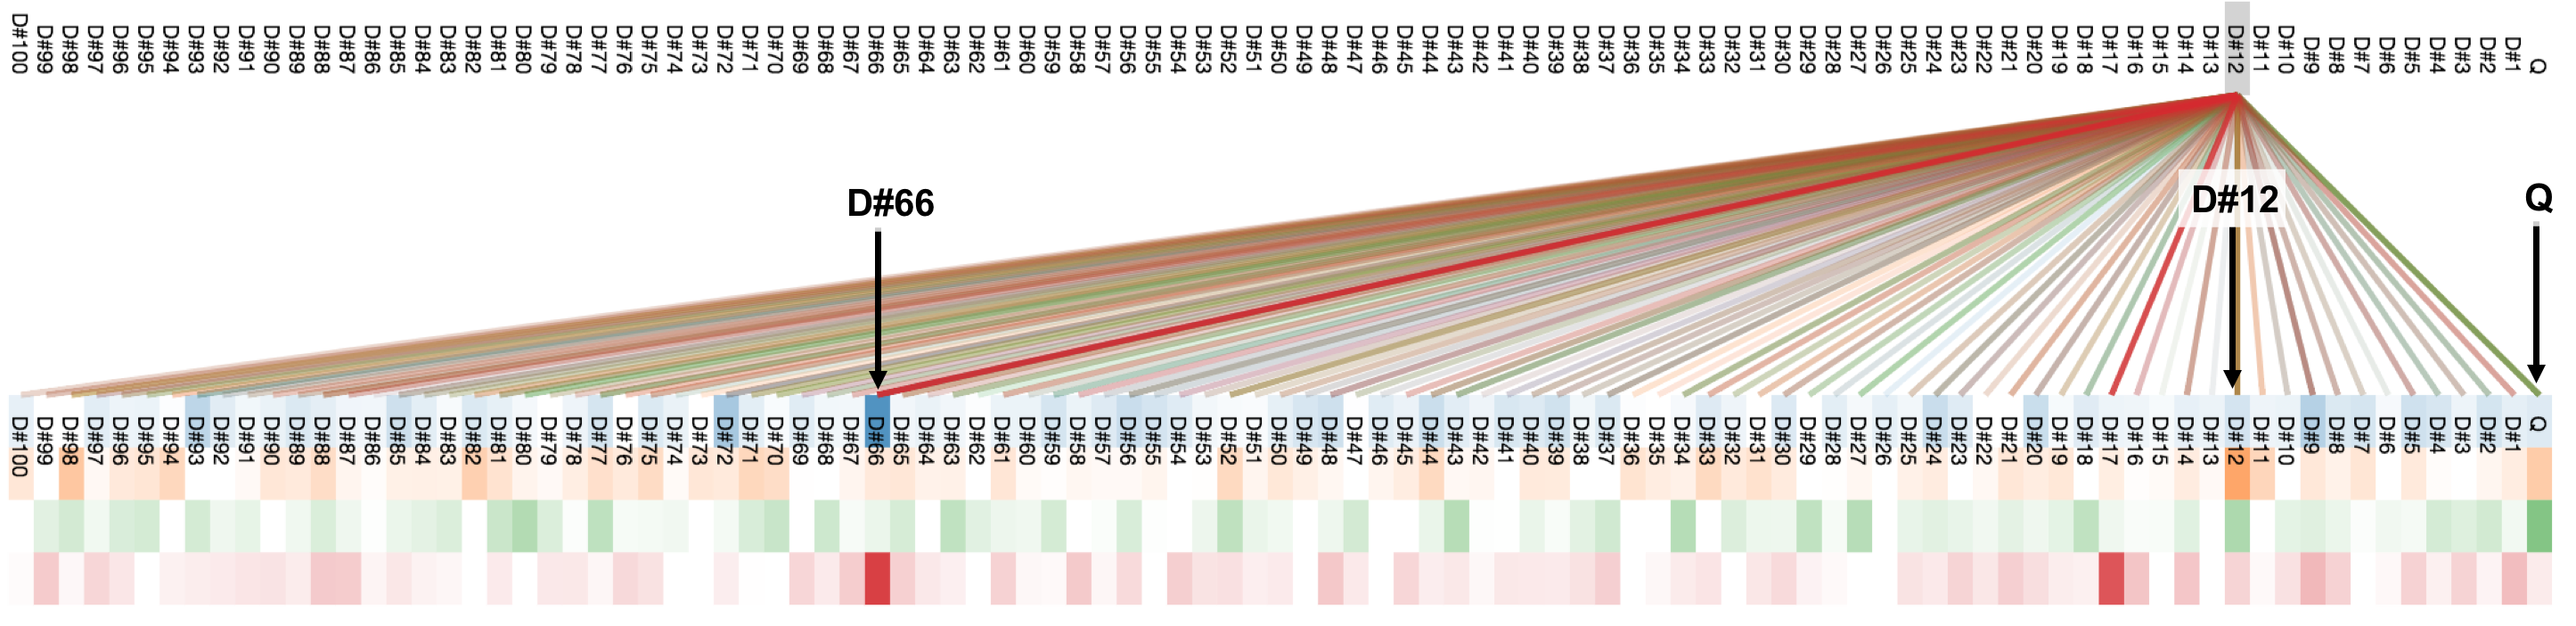
\includegraphics[width=\textwidth]{04-part-03/chapter-06/figs_and_tables/fig_att_tracrnet_step3.png}
        \caption{\label{fig:attention_vis_a}Attention distribution %over different documents and the question 
        when transforming the document at rank 12, in step\#3 of multihop reasoning.}
    \end{subfigure}%
    \vfill
    \begin{subfigure}[t]{\textwidth}
        \centering
        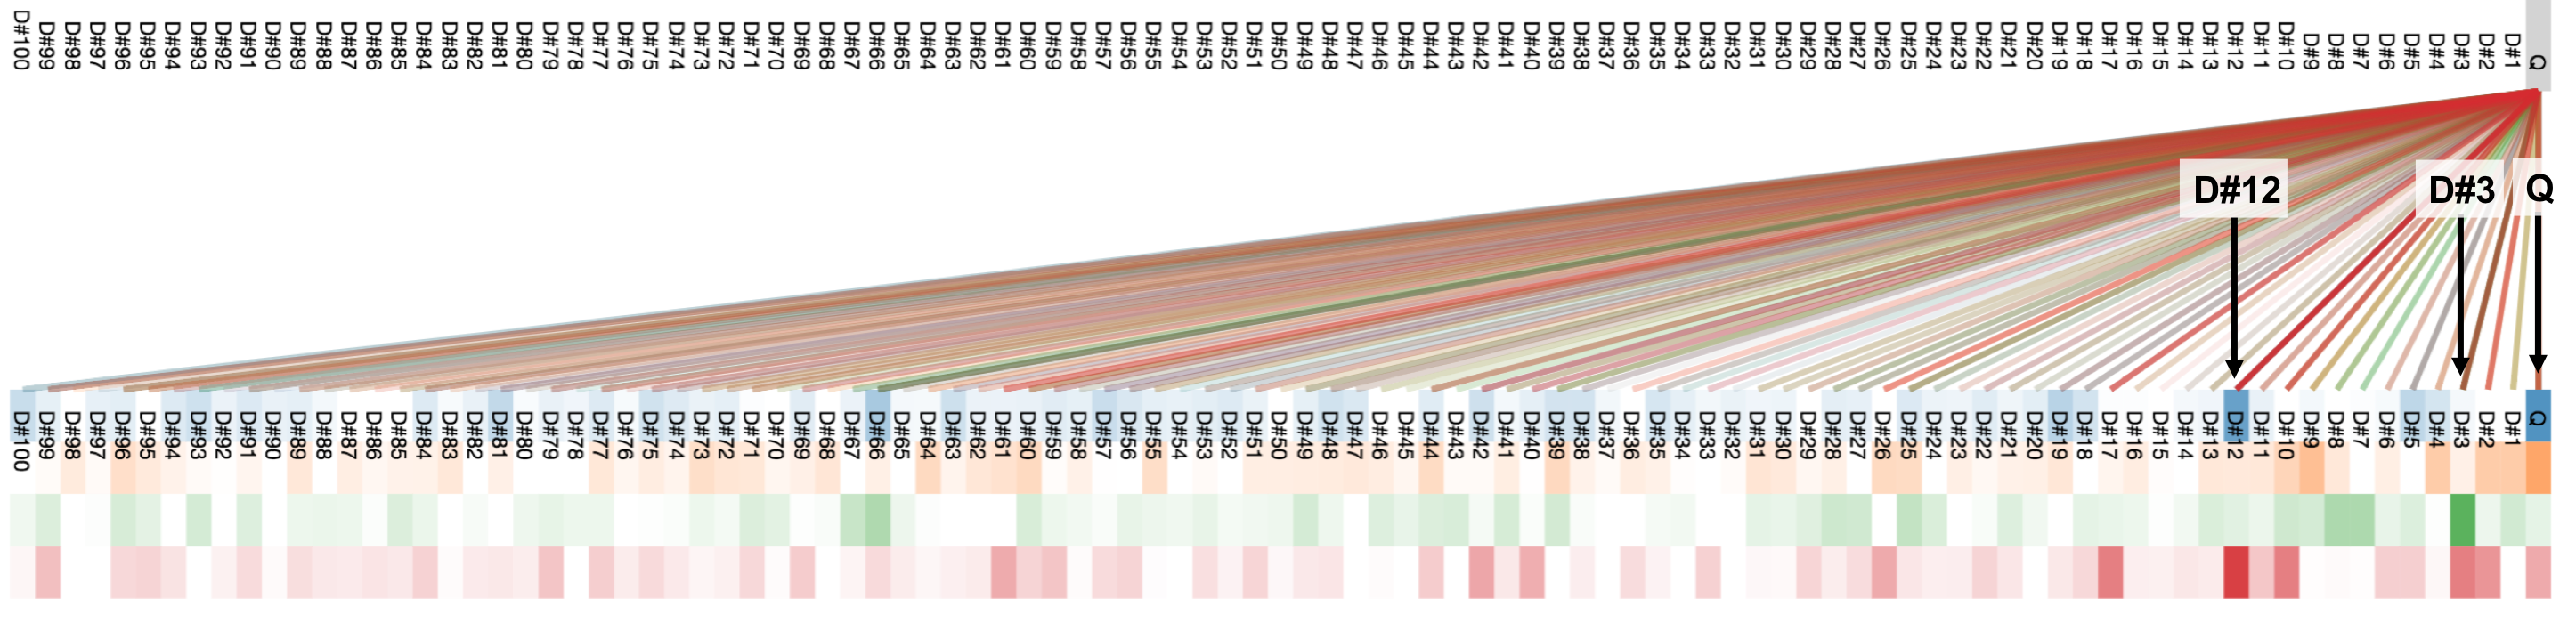
\includegraphics[width=\textwidth]{04-part-03/chapter-06/figs_and_tables/fig_att_tracrnet_step7.png}
        \caption{\label{fig:attention_vis_b}Attention distribution %over different documents and the question 
        when transforming the question, in step\#7 of multihop reasoning.}
    \end{subfigure}
     \caption{Visualization  of multi-head self-attention on Multihop Reasoning layer of \tracrnet. 
     (Best viewed in color.)}
     \label{fig:attention_vis}
\end{figure}

On all measures and datasets, the performance drops when we remove the \emph{Multihop Reasoning} layer. 
The drop in the performance is larger on the Quasar-T dataset than on the SearchQA dataset.
We noticed that trivia questions in Quasar-T, in many cases, contain clauses that should be considered together with and/or operations to be able to give the correct answer. 
For instance, to answer the question ``What Australian food was discovered by John McAdam,'' we should consider that ``the food is Australian'' \emph{and} ``the food is discovered by John McAdam.'' 
In this situation, the chance of having multiple documents each containing one of these facts increases. 
Thus, having multiple supporting documents and the need for reasoning (similar to Example~\ref{fig:example}) will be the exact point where the advantage of the \emph{Multihop Reasoning} layer kicks in.

Another observation here is that when we remove the \emph{Multihop Reasoning} layer, passing word-level embeddings from the encoder to the decoder leads to better EM scores, but not to improved F1 scores. 
The main reason is that, in this situation, access to the input words from the decoder is more explicit. 
This helps the model to get closer to answer extraction than pure answer generation.

For the test example that is presented in Figure~\ref{fig:example}, we observed that all baseline models output ``Georges Braque'' which is extracted from the document at rank~1. 
However, unlike all the baselines, \tracrnet returns the correct answer. 
We looked into the attention distributions in the \emph{Multihop Reasoning} layer of \tracrnet at different steps (of the employed Universal Transformer with 12 depth-wise recurrent steps). 
We were able to find a relation between attention distributions and the reasoning steps that are needed to give the correct answer to this question. 
We illustrate this in Figure~\ref{fig:attention_vis}.

Figure~\ref{fig:attention_vis_a} presents the attention distribution over all documents and the question while encoding the document at rank~12 at step~3. 
\tracrnet has a high level of attention for the document at rank~66 using heads~1 and~4 (blue and red) as well as for the question using head~3 (green) while transforming the document at rank~12. 
This is in accordance with the fact that the model first needs to update the information encoded in the document at rank 12 with the fact that ``Malaga is a city in Spain'' from the document at rank~66. 
Later, at step~7, while encoding the question (Figure~\ref{fig:attention_vis_b}), \tracrnet attends over document 12, which has information about ``Picasso who is a Spanish artist'' (updated in step~3) using heads~1 and~4 and document~3, which contains information about ``Picasso as a co-founder of Cubism'' using head~2 (green). 

\subsubsection{Impact of the number of documents}
As we explained before, unlike most of the previous work that filters candidate documents and narrows down the set of documents under consideration to either a single document or a small set of highly relevant documents before applying an answer extractor to them, \tracrnet uses the full set of candidate documents retrieved by the search engine during the entire process of generating the answer. 
This is of great advantage as our analysis shows that, for some questions, the correct answer can only be extracted when considering information from low-ranked documents that are not immediately relevant to the question.
However, this can potentially come at the cost of (1)~efficiency, as we need to process a larger input, and of (2)~performance, as there will be more noisy and non-relevant documents when we go down the ranked list of candidate documents. 
%
Making use of self-attentive feed-forward neural networks as building blocks of \tracrnet brings the ability of full per-symbol parallelization and leads to an enormous speedup on encoding the input documents. This lets the model encode a larger set of candidate documents efficiently. 

\begin{figure}[!t]
 \centering
 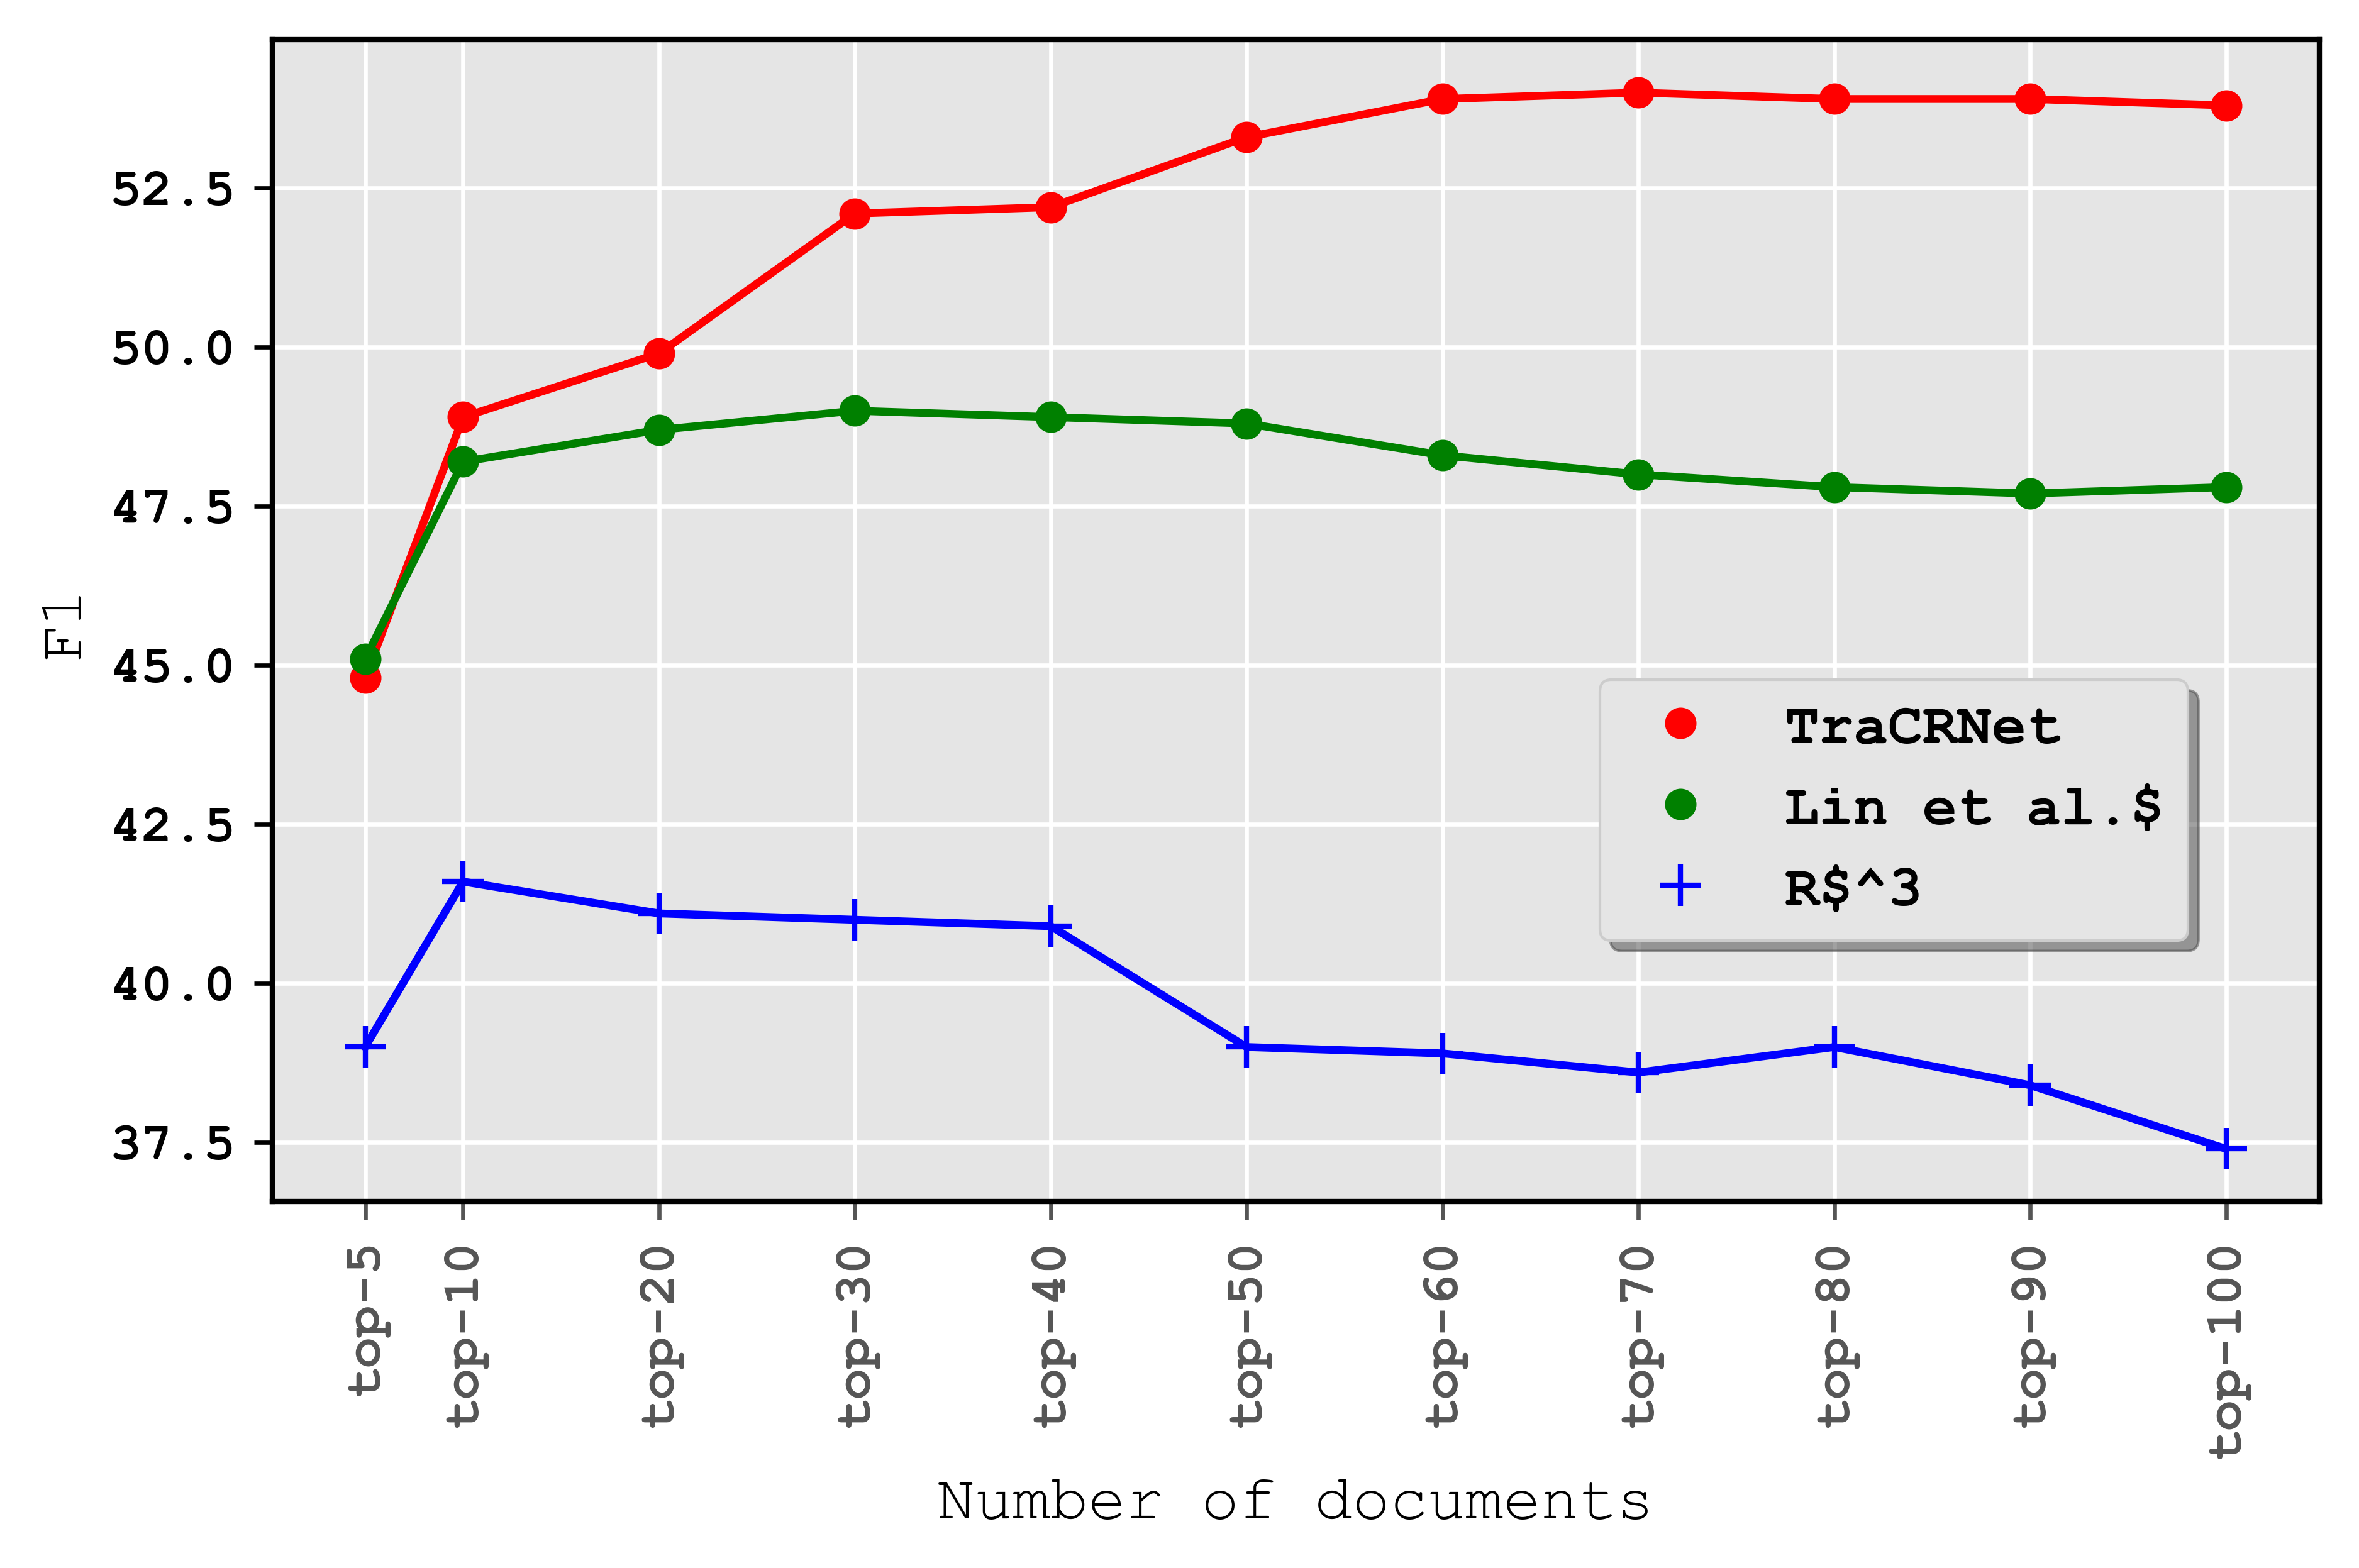
\includegraphics[width=0.6\textwidth]{04-part-03/chapter-06/figs_and_tables/plot_different_num_docs.png}
  %\vspace{5pt}
 \caption{Performance in terms of F1 of \tracrnet and baselines (R$^3$~\citep{wang2017r} and \citet{lin2018denoising}'s model) with different numbers of candidate documents on Quasar-T dataset.}
 \label{fig:diff_num_docs}
\end{figure}

To study how the performance of \tracrnet is affected by the number of candidate documents, we train and evaluate \tracrnet as well as R$^3$~\citep{wang2017r} and \citet{lin2018denoising}'s model on the Quasar-T dataset, using different numbers of candidate documents associated with each question.\footnote{In this experiment, we just change the initial number of candidates, but we train baseline models with their original setups and do not impose any assumption (e.g., fixing the candidate list) on them.}
%
Figure~\ref{fig:diff_num_docs} presents the performance of these models when they are fed with the top-5, top-10, \ldots, top-100 retrieved documents. 
%
As can be seen, although \citet{lin2018denoising}'s model is pretty good at staying robust when noise increases (it is designed to learn from distant supervision), increasing the number of candidate documents eventually leads to a small drop in performance of both baselines due to the noise in the low-ranked documents. 
However, \tracrnet not only controls the effect of noisy low-ranked documents by calibrating their effect on inferring the final answer through self-attention, but it also keeps improving as we increase the number of documents as it can exploit any useful information contained in low-ranked documents which can help better understand the question or perform reasoning.





\section{Conclusion}
In this chapter we focused on addressing \textbf{\resqname{c6}}: ``\emph{\resqcontent{c6}}''.
We introduced the Universal Transformer to address \textbf{\resqname{c6.1}}, a generalization of the Transformer model that extends its theoretical capabilities, by introducing the recurrent inductive bias in depth. 
We have employed the Universal Transformer in on a wide range of challenging sequence modeling tasks, such as language understanding but also a variety of algorithmic tasks, to address \textbf{\resqname{c6.2}} and showed that it produces state-of-the-art results by addressing a key shortcoming of the standard Transformer. The Universal Transformer combines the following key properties into one model:

\textbf{Weight sharing}: Following intuitions behind weight sharing found in CNNs and RNNs, we extend the Transformer with a simple form of weight sharing that strikes an effective balance between inductive bias and model expressivity, which we show extensively on both small and large-scale experiments.

\textbf{Conditional computation}: In our goal to build a computationally universal machine, we equipped the Universal Transformer with the ability to halt or continue computation through a recently introduced mechanism, which shows stronger results compared to the fixed-depth Universal Transformer.

By adding computational capacity and recurrence in processing depth, we hope that further improvements beyond the basic Universal Transformer presented here will help us build learning algorithms that are both more powerful, data efficient, and generalize beyond the current state-of-the-art.

In Part~\ref{part3} of the thesis, we focused on addressing \textbf{\resqname{p3}}: ``\emph{\resqcontent{p3}}''.
we explored the idea of injecting inductive biases into learning algorithms to improve their data-efficiency and generalization. This in fact is defining an innate prior knowledge for the learning algorithms that can eventually help overcoming the challenging problem of poverty of stimulus.



\bookmarksetup{startatroot} % Lift from parts
\addtocontents{toc}{\bigskip} % skip

\chapter{Conclusion}
The success of today's machine learning algorithms in complex tasks depends strongly on the availability of large scale high quality labeled data. In practice, however, for many applications and domains, the available training data is limited or noisy and it is difficult to build machines that can learn with such imperfect training data.
%
In contrast, humans are capable of uncovering the underlying concepts, relations, and structure of the sparsely observed data with variable quality and use that knowledge to go far beyond the scarcity of the data and routinely make successful generalizations based on them.

The argument of \emph{poverty of stimulus}~\citep{chomsky1980rules} in human learning suggests that the observed data is not rich enough for selecting a correct target hypothesis without posing an a priori knowledge~\citep{chomsky1971problems}.
%
In par with this, when designing machine learning algorithms, pure \emph{data-driven} learning, which relies only on previous experience, does not seem to be able to learn generalizable solutions. Similar to human's \emph{innately primed} learning, having a part of the knowledge encoded in the learning algorithms in the form of strong or weak biases, can help them learn solutions that better generalize to unseen samples~\citep{Mitchell80theneed, Mitchell:1997:ML}.

Here, in this thesis, we focused on this problem of poverty of stimulus for learning algorithms. We argued that even noisy and limited signals can contain a great deal of valid information that can be incorporated along with prior knowledge and biases that are encoded into learning algorithms in order to solve complex problems. 
We study how to improve the learning with imperfect supervision signal in the context of language understanding and sequence modeling tasks.


\section{Research Questions and Conclusions}
In this thesis, we focused on learning with imperfect supervision. We referred to ``\emph{imperfect supervision}'' as a general term covering a variety of situations where the learning process is based on imperfect training examples. This imperfection can be in the number or coverage of training examples like learning from \emph{incomplete supervision}, where only a limited subset of data is labeled or no labeled data is available. The imperfection can refer to the labeling process like in \emph{inexact supervision} where only coarse-grained annotations are provided or \emph{inaccurate supervision} where the given labels are noisy and they are not always ground truth~\citep{zhou2018brief}. We also consider situations where not only the labels in the training data but also feature vectors can be limited, noisy, or subject to change during time.

We formulated the main research question of the thesis as:
%
\resq{main}
%

We broke down our main research question into three questions and addressed each of them in each part of this thesis.
The first question, that we addressed in Part~\ref{part1} of the thesis, was:
%
\resq{p1}

In Part~\ref{part1}, we focused on learning representations for the entities and abstract concepts, like topical relevance, a political conviction, etc., given a data in which the features and labels can be noisy or subject to change during time.

First, in Chapter~\ref{chap:2} inspired by the discussion on the early work by~\citet{Luhn:1958} about \emph{significant words} we introduced \emph{\swlms}\ (\acswlm) that estimate a representation for an entity or concept that is associated with a set of textual documents in a way that the estimated representation captures significant features by avoiding the distracting effect of common features as well as rare features. We evaluated \acswlm on a set of problems including (pseudo-)relevance feedback in document ranking and group profiling in contextual suggestion and recommendation and showed that we can improve the quality and robustness of representations by making them less independent on general or specific features, but more rely on significant features.

Then, in Chapter~\ref{chap:3}, we extended our discussions in Chapter~\ref{chap:2} to hierarchical structures and introduced \hswlms (\achswlm) for estimating separable representations for hierarchical entities. We demonstrated that based on the ranking and classification principles, the \emph{separation property} in the data representation is a desirable foundational property which leads to separability of scores and consequently improves the accuracy of classifiers' decisions. 

We showed that in order to have horizontally and vertically separable representations for hierarchically structured data, they should capture all, and only, the essential features of the entities taking their position in the hierarchy into account, which is the key idea of \achswlm. We evaluated the performance of classification over time using separable representations learned by \achswlm and showed that separability makes the model more robust and transferable over time by filtering out non-essential and non-stable features.

\textbf{The main conclusion of Part~\ref{part1}} is that incorporating prior knowledge can help improve the robustness of the outcome of the learning process in noisy and variable environments. We showed that taking the general structure of the data as prior knowledge, which is, in fact, a form of inductive bias, can help to learn representations that are not only effective but also less affected by noisy factors in the data.

\bigskip
The second question, that we addressed in Part~\ref{part2} of the thesis, was:
%
\resq{p2}

In Part~\ref{part2}, we focused on how to augment the training data using a vast amount of data that are not hand-labeled, but weakly annotated using, for instance, a heuristic function. We discuss how to train learning algorithms using such weak labels and how to learn properties of the weakly annotated data, like the quality of labels and incorporate those in the learning process.  

First, in Chapter~\ref{chap:4}, we proposed to use unsupervised methods in order to programmatically generate large amounts of training data, as weakly annotated data, to train effective neural ranking models. We focus on the task of assessing the topical relevance, i.e., ranking documents given a query. We examined various neural ranking models with different ranking architectures and objectives, and different input representations.

We found that providing the network with raw data and letting the network to learn the features that matter, gives the network a chance of learning how to ignore imperfection in the training data. Also we showed that in the case of having weakly annotated training data, by targeting some explicit labels from the data, we may end up with a model that learned to express the data very well, but is incapable of going beyond it. We also observed that when learning by weakly annotated data, it is crucial to provide the network with a considerable amount of diverse training examples to help the model learn at the edge of its capacity.

Then, in Chapter~\ref{chap:5}, we proposed a set of systematic approaches that are tasks and architecture independent and can meta-learn the quality of the labels and explicitly control the learning process with respect to the estimated qualities. We introduced two semi-supervised learning approaches in the presence of weakly labeled data: Learning from Controlled Weak Supervision (\cws) and \fwlfulllc (\fwl).

\cws is a meta-learning approach that unifies learning to estimate the confidence score of weak annotations and training neural networks to learn a target task with controlled weak supervision, i.e., using weak labels to updating the parameters but taking their estimated confidence scores into account. \fwl is a student-teacher framework in which the student network is in charge of learning a target task given a vast amount of samples with weak labels associated with fidelity scores that are generated by the teacher network.  We applied both \cws and \fwl to document ranking and sentiment classification and empirically verified that they improve the learning process in terms of performance and convergence time. 

\textbf{The main conclusion of part~\ref{part2}} is that we can design models that are capable of learning from weakly annotated data by defining proper training objectives. We also found that we can use the data to metal-learn some properties of the data, like the quality of labels and incorporate these properties in the learning process.

\bigskip
The last question, that we addressed in Part~\ref{part3} of the thesis, was:
%
\resq{p3}

In Part~\ref{part3}, we focused on some of the sequence processing neural networks and study the role of inductive biases, like recurrent inductive bias, on the generalization and data efficiency of these models on different language understanding and sequence modeling tasks.

In Chapter~\ref{chap:6}, we argue that the lack of recurrent inductive bias in feed-forward self-attentive models, like Transformer, can lead to the failure of the model on complex reasoning tasks with limited data, algorithmic tasks where length generalization over training samples is needed, and structured language understanding tasks. We proposed Universal Transformer, a self-attentive concurrent-recurrent sequence model, in which we introduce recurrence in depth by repeatedly modifying a series of vector representations for each position of the sequence in parallel. The key idea of the universal transformer is sharing the parameters across the layers which forms a recurrent inductive bias in depth and saves massively on the number of parameters and leads to a more data efficient model. 

We also discussed other assumptions that encoding them in the model as inductive biases can help extrapolating from training data and better generalizing at test time.  We also introduced some variants of the Universal Transformer with conditional computations and showed that it can achieve stronger results compared to the fixed-depth Universal Transformer.

\textbf{The main conclusion of Part~\ref{part3}} is that injecting inductive biases into learning algorithms can improve their data-efficiency and generalization. These inductive biases are in fact innate prior knowledge for the learning algorithms that can eventually help overcoming the challenging problem of poverty of stimulus.

\bigskip
As the \textbf{general conclusion} of this thesis, we found that we can improve the process of learning with imperfect supervision by i) \emph{employing the prior knowledge in learning algorithms} (Part~\ref{part1}), ii) \emph{augmenting data and meta-learning how to better use the data} (Part~\ref{part1}), and iii) \emph{introducing inductive biases to learning algorithms} (Part~\ref{part1}). 
%
These general ideas are, in fact, the key ingredients for building any learning algorithms that can generalize beyond (imperfections in) the observed data ~\citep{Mitchell80theneed}.

\section{Towards Building Machines that Deal with Poverty of Stimulus}

There has been a long discussion between empiricists and rationalists in the context of human learning concerning the extent to which we are dependent on our experiences and observations in our effort to gain knowledge.  
%
Empiricists claim that sensory observations (data) are the ultimate source of all our concepts and knowledge, while rationalists claim that there are significant ways in which our concepts and knowledge are gained independently of our experiences and observations. 

A similar discussion has been raised in machine learning in the context of learning algorithms.
%
Some machine learning researchers believe that the intrinsic complexity of the world means we should not build any prior knowledge into our systems: ``Seeking an improvement that makes a difference in the shorter term, researchers seek to leverage their human knowledge of the domain, but the only thing that matters in the long run is the leveraging of computation.''%\citep{TheBitterLesson}
\footnote{``The Bitter Lesson'' by Rich Sutton: \url{http://www.incompleteideas.net/IncIdeas/BitterLesson.html}}

Some other machine learning researchers, on the other hand, emphasize on the fact that ``there are no predictions without assumptions, no generalization without inductive bias'' and believe that the complexity of the world, as the mater of fact, leads to crippling intractability for the approaches on which empiricists proposes to rely on and argue that only with the right prior knowledge and the right inductive biases, we can ever get a handle on that complexity.
%~\citep{maxblogpost, Mitchell:1997:ML}.
\footnote{``Do we still need models or just more data and compute?'' by MAx Welling: \url{https://staff.fnwi.uva.nl/m.welling/wp-content/uploads/Model-versus-Data-AI-1.pdf}}

In practice, we do not apply either rigorous empiricist or rationalist approaches in machine learning.  When we pursue more explanatory rationalist approaches, we always recognize the importance of observations and the data as the means by which reality affects our understanding.  When taking a data-driven approach, we make use of reasoning at least in the act of observing data, i.e., choices such as how data is selected, assumptions we make, biases to our algorithms, and the overall architectures of our solution. 

We believe that in order to build machines that can create knowledge a truce between these two main approaches is essential.
There is no doubt that the success of deep learning is very much a success of scale and in general, machine learning methods that survive the test of time and make breakthrough progress tend to scale.
But incorporating knowledge or inductive biases has its own success stories and the question here is more about ``what'' that knowledge or biases should be and ``when'' and ``how'' it should be incorporated. 

While finding the right inductive biases is hard, they can enable progress on intractable problems or situations where we cannot rely on arbitrarily scaling of computation such as settings with noisy or limited data, which characterizes most real-world applications. 
Besides, scalability can be defined in many dimensions, If a method is ``scalable'' with more data and computation, it has the chance of succeeding only in a subset of problems that we can gather infinite data for them. 
However, you can define the ``scale'', as in ``scale to new problems'', which is, in fact, the ability of generalization, where inductive biases can play crucial roles to achieve it, especially when considering the problem of poverty of stimulus.


\bigskip
% closing paragraph
We are enthusiastic about the recent developments on machine learning models that are able to learn with imperfect supervision. 
By combining the ideas around how to incorporate general prior knowledge, how to better use the data and meta learn its properties, and how to injecting right inductive biases, we hope that further improvements presented in this thesis will help us build learning algorithms that are more powerful, more data efficient, and more generalizable and in a bigger picture, help machines to get closer to the human-level intelligence. 



\appendix
%\include{thesis_appendix}

%%  \include the `end matter'
\cleardoublepage % if you are so inclined
\bibliographystyle{apalike}
\bibliography{thesis_ref}

% \begin{theindex}
By preference, your dissertation\linebreak
should contain an index. Instructions
on how to produce an index can be
found on pages 77--79 of the
 \LaTeX\ manual. You may specify
an index as follows:\\[2ex]
\verb|  \begin{theindex}|\\
\verb|    <your list of entries>|\\
\verb|  \end{theindex}|
\end{theindex}


% \samenvatting
According to both ILLC standards and UvA promotion regulations,
a chapter containing a summary in
Dutch of your dissertation should always be included.
It is specified by:
\begin{verbatim}
  \samenvatting
    <your Samenvatting>
\end{verbatim}

% \abstract
Humans learn to solve complex problems and uncover underlying concepts and relations given limited, noisy or inconsistent observations and draw successful generalizations based on them. This rests largely on the \emph{poverty of the stimulus} argument, or what is sometimes called \emph{Plato’s problem}~\citep{chomsky1986knowledge}: ``How do we know so much when the evidence available to us is so meagre?''

In contrast, the success of today's data-driven machine learning models is often strongly correlated with the amount of available high quality labeled data~\citep{halevy2009unreasonable,sun2017revisiting} and teaching machines using \emph{imperfect supervision} remains a key challenge. In practice, however, for many applications, large-scaled high-quality training data is not available, which highlights the increasing need for building models with the ability to learn complex tasks with imperfect supervision, i.e., where the learning process is based on imperfect training samples~\citep{zhou2018brief}.

When designing learning algorithms, pure \emph{data-driven} learning, which relies only on previous experience, does not seem to be able to learn generalizable solutions~\citep{Mitchell80theneed}. Similar to human's \emph{innately primed} learning, having part of the knowledge encoded in the learning algorithms in the form of strong or weak biases, can help learning solutions that better generalize to unseen samples~\citep{Mitchell:1997:ML}.

In this thesis, we focus on the problem of the \textbf{poverty of stimulus for learning algorithms}. We argue that even noisy and limited signals can contain a great deal of valid information that can be incorporated along with prior knowledge and biases that are encoded into learning algorithms in order to solve complex problems. We improve the process of learning with imperfect supervision by (i) \emph{employing  prior knowledge in learning algorithms}, (ii) \emph{augmenting data and learning to learn how to better use the data}, and (iii) \emph{introducing inductive biases to learning algorithms} . 
%
These general ideas are, in fact, the key ingredients for building any learning algorithms that can generalize beyond (imperfections in) the observed data ~\citep{Mitchell80theneed}.

We concentrate on language understanding and reasoning, as one of the extraordinary cognitive abilities of humans, as well as a pivotal problem in artificial intelligence. We try to improve the learning process, in more principled ways than ad-hoc and domain or task-specific tricks to improve the output. We investigate our ideas on a wide range of sequence modeling and language understanding tasks.




%%  finally, \include the list of previous ILLC dissertations

\cleardoublepage % if you are so inclined
\pagestyle{empty}

\noindent
{\em Titles in the ILLC Dissertation Series:}

\newcommand{\illcpublication}[3]{\item[ILLC #1: ]{\bf #2}\\{\em #3}}

\begin{list}{}{ \settowidth{\leftmargin}{ILL}
		\setlength{\rightmargin}{0in}
		\setlength{\labelwidth}{\leftmargin}
		\setlength{\labelsep}{0in}
}

\illcpublication{DS-2009-01}{Jakub Szymanik}{Quantifiers in TIME and SPACE. Computational Complexity of Generalized Quantifiers in Natural Language}
\illcpublication{DS-2009-02}{Hartmut Fitz}{Neural Syntax}
\illcpublication{DS-2009-03}{Brian Thomas Semmes}{A Game for the Borel Functions}
\illcpublication{DS-2009-04}{Sara L. Uckelman}{Modalities in Medieval Logic}
\illcpublication{DS-2009-05}{Andreas Witzel}{Knowledge and Games: Theory and Implementation}
\illcpublication{DS-2009-06}{Chantal Bax}{Subjectivity after Wittgenstein. Wittgenstein's embodied and embedded subject and the debate about the death of man.}
\illcpublication{DS-2009-07}{Kata Balogh}{Theme with Variations. A Context-based Analysis of Focus}
\illcpublication{DS-2009-08}{Tomohiro Hoshi}{Epistemic Dynamics and Protocol Information}
\illcpublication{DS-2009-09}{Olivia Ladinig}{Temporal expectations and their violations}
\illcpublication{DS-2009-10}{Tikitu de Jager}{"Now that you mention it, I wonder...": Awareness, Attention, Assumption}
\illcpublication{DS-2009-11}{Michael Franke}{Signal to Act: Game Theory in Pragmatics}
\illcpublication{DS-2009-12}{Joel Uckelman}{More Than the Sum of Its Parts: Compact Preference Representation Over Combinatorial Domains}
\illcpublication{DS-2009-13}{Stefan Bold}{Cardinals as Ultrapowers. A Canonical Measure Analysis under the Axiom of Determinacy.}
\illcpublication{DS-2010-01}{Reut Tsarfaty}{Relational-Realizational Parsing}
\illcpublication{DS-2010-02}{Jonathan Zvesper}{Playing with Information}
\illcpublication{DS-2010-03}{Cédric Dégremont}{The Temporal Mind. Observations on the logic of belief change in interactive systems}
\illcpublication{DS-2010-04}{Daisuke Ikegami}{Games in Set Theory and Logic}
\illcpublication{DS-2010-05}{Jarmo Kontinen}{Coherence and Complexity in Fragments of Dependence Logic}
\illcpublication{DS-2010-06}{Yanjing Wang}{Epistemic Modelling and Protocol Dynamics}
\illcpublication{DS-2010-07}{Marc Staudacher}{Use theories of meaning between conventions and social norms}
\illcpublication{DS-2010-08}{Amélie Gheerbrant}{Fixed-Point Logics on Trees}
\illcpublication{DS-2010-09}{Gaëlle Fontaine}{Modal Fixpoint Logic: Some Model Theoretic Questions}
\illcpublication{DS-2010-10}{Jacob Vosmaer}{Logic, Algebra and Topology. Investigations into canonical extensions, duality theory and point-free topology.}
\illcpublication{DS-2010-11}{Nina Gierasimczuk}{Knowing One's Limits. Logical Analysis of Inductive Inference}
\illcpublication{DS-2010-12}{Martin Mose Bentzen}{Stit, Iit, and Deontic Logic for Action Types}
\illcpublication{DS-2011-01}{Wouter M. Koolen}{Combining Strategies Efficiently: High-Quality Decisions from Conflicting Advice}
\illcpublication{DS-2011-02}{Fernando Raymundo Velazquez-Quesada}{Small steps in dynamics of information}
\illcpublication{DS-2011-03}{Marijn Koolen}{The Meaning of Structure: the Value of Link Evidence for Information Retrieval}
\illcpublication{DS-2011-04}{Junte Zhang}{System Evaluation of Archival Description and Access}
\illcpublication{DS-2011-05}{Lauri Keskinen}{Characterizing All Models in Infinite Cardinalities}
\illcpublication{DS-2011-06}{Rianne Kaptein}{Effective Focused Retrieval by Exploiting Query Context and Document Structure}
\illcpublication{DS-2011-07}{Jop Briët}{Grothendieck Inequalities, Nonlocal Games and Optimization}
\illcpublication{DS-2011-08}{Stefan Minica}{Dynamic Logic of Questions}
\illcpublication{DS-2011-09}{Raul Andres Leal}{Modalities Through the Looking Glass: A study on coalgebraic modal logic and their applications}
\illcpublication{DS-2011-10}{Lena Kurzen}{Complexity in Interaction}
\illcpublication{DS-2011-11}{Gideon Borensztajn}{The neural basis of structure in language}
\illcpublication{DS-2012-01}{Federico Sangati}{Decomposing and Regenerating Syntactic Trees}
\illcpublication{DS-2012-02}{Markos Mylonakis}{Learning the Latent Structure of Translation}
\illcpublication{DS-2012-03}{Edgar José Andrade Lotero}{Models of Language: Towards a practice-based account of information in natural language}
\illcpublication{DS-2012-04}{Yurii Khomskii}{Regularity Properties and Definability in the Real Number Continuum: idealized forcing, polarized partitions, Hausdorff gaps and mad families in the projective hierarchy.}
\illcpublication{DS-2012-05}{David García Soriano}{Query-Efficient Computation in Property Testing and Learning Theory}
\illcpublication{DS-2012-06}{Dimitris Gakis}{Contextual Metaphilosophy - The Case of Wittgenstein}
\illcpublication{DS-2012-07}{Pietro Galliani}{The Dynamics of Imperfect Information}
\illcpublication{DS-2012-08}{Umberto Grandi}{Binary Aggregation with Integrity Constraints}
\illcpublication{DS-2012-09}{Wesley Halcrow Holliday}{Knowing What Follows: Epistemic Closure and Epistemic Logic}
\illcpublication{DS-2012-10}{Jeremy Meyers}{Locations, Bodies, and Sets: A model theoretic investigation into nominalistic mereologies}
\illcpublication{DS-2012-11}{Floor Sietsma}{Logics of Communication and Knowledge}
\illcpublication{DS-2012-12}{Joris Dormans}{Engineering emergence: applied theory for game design}
\illcpublication{DS-2013-01}{Simon Pauw}{Size Matters: Grounding Quantifiers in Spatial Perception}
\illcpublication{DS-2013-02}{Virginie Fiutek}{Playing with Knowledge and Belief}
\illcpublication{DS-2013-03}{Giannicola Scarpa}{Quantum entanglement in non-local games, graph parameters and zero-error information theory}
\illcpublication{DS-2014-01}{Machiel Keestra}{Sculpting the Space of Actions. Explaining Human Action by Integrating Intentions and Mechanisms}
\illcpublication{DS-2014-02}{Thomas Icard}{The Algorithmic Mind: A Study of Inference in Action}
\illcpublication{DS-2014-03}{Harald A. Bastiaanse}{Very, Many, Small, Penguins}
\illcpublication{DS-2014-04}{Ben Rodenhäuser}{A Matter of Trust: Dynamic Attitudes in Epistemic Logic}
\illcpublication{DS-2015-01}{María Inés Crespo}{Affecting Meaning. Subjectivity and evaluativity in gradable adjectives.}
\illcpublication{DS-2015-02}{Mathias Winther Madsen}{The Kid, the Clerk, and the Gambler - Critical Studies in Statistics and Cognitive Science}
\illcpublication{DS-2015-03}{Shengyang Zhong}{Orthogonality and Quantum Geometry: Towards a Relational Reconstruction of Quantum Theory}
\illcpublication{DS-2015-04}{Sumit Sourabh}{Correspondence and Canonicity in Non-Classical Logic}
\illcpublication{DS-2015-05}{Facundo Carreiro}{Fragments of Fixpoint Logics: Automata and Expressiveness}
\illcpublication{DS-2016-01}{Ivano A. Ciardelli}{Questions in Logic}
\illcpublication{DS-2016-02}{Zoé Christoff}{Dynamic Logics of Networks: Information Flow and the Spread of Opinion}
\illcpublication{DS-2016-03}{Fleur Leonie Bouwer}{What do we need to hear a beat? The influence of attention, musical abilities, and accents on the perception of metrical rhythm}
\illcpublication{DS-2016-04}{Johannes Marti}{Interpreting Linguistic Behavior with Possible World Models}
\illcpublication{DS-2016-05}{Phong Lê}{Learning Vector Representations for Sentences - The Recursive Deep Learning Approach}
\illcpublication{DS-2016-06}{Gideon Maillette de Buy Wenniger}{Aligning the Foundations of Hierarchical Statistical Machine Translation}
\illcpublication{DS-2016-07}{Andreas van Cranenburgh}{Rich Statistical Parsing and Literary Language}
\illcpublication{DS-2016-08}{Florian Speelman}{Position-based Quantum Cryptography and Catalytic Computation}
\illcpublication{DS-2016-09}{Teresa Piovesan}{Quantum entanglement: insights via graph parameters and conic optimization}
\illcpublication{DS-2016-10}{Paula Henk}{Nonstandard Provability for Peano Arithmetic. A Modal Perspective}
\illcpublication{DS-2017-01}{Paolo Galeazzi}{Play Without Regret}
\illcpublication{DS-2017-02}{Riccardo Pinosio}{The Logic of Kant's Temporal Continuum}
\illcpublication{DS-2017-03}{Matthijs Westera}{Exhaustivity and intonation: a unified theory}
\illcpublication{DS-2017-04}{Giovanni Cinà}{Categories for the working modal logician}
\illcpublication{DS-2017-05}{Shane Noah Steinert-Threlkeld}{Communication and Computation: New Questions About Compositionality}
\illcpublication{DS-2017-06}{Peter Hawke}{The Problem of Epistemic Relevance}
\illcpublication{DS-2017-07}{Aybüke Özgün}{Evidence in Epistemic Logic: A Topological Perspective}
\illcpublication{DS-2017-08}{Raquel Garrido Alhama}{Computational Modelling of Artificial Language Learning: Retention, Recognition \& Recurrence}
\illcpublication{DS-2017-09}{Miloš Stanojević}{Permutation Forests for Modeling Word Order in Machine Translation}
\illcpublication{DS-2018-01}{Berit Janssen}{Retained or Lost in Transmission? Analyzing and Predicting Stability in Dutch Folk Songs}
\illcpublication{DS-2018-02}{Hugo Huurdeman}{Supporting the Complex Dynamics of the Information Seeking Process}
\illcpublication{DS-2018-03}{Corina Koolen}{Reading beyond the female: The relationship between perception of author gender and literary quality}
\illcpublication{DS-2018-04}{Jelle Bruineberg}{Anticipating Affordances: Intentionality in self-organizing brain-body-environment systems}
\illcpublication{DS-2018-05}{Joachim Daiber}{Typologically Robust Statistical Machine Translation: Understanding and Exploiting Differences and Similarities Between Languages in Machine Translation}
\illcpublication{DS-2018-06}{Thomas Brochhagen}{Signaling under Uncertainty}
\illcpublication{DS-2018-07}{Julian Schlöder}{Assertion and Rejection}
\illcpublication{DS-2018-08}{Srinivasan Arunachalam}{Quantum Algorithms and Learning Theory}
\illcpublication{DS-2018-09}{Hugo de Holanda Cunha Nobrega}{Games for functions: Baire classes, Weihrauch degrees, transfinite computations, and ranks}
\illcpublication{DS-2018-10}{Chenwei Shi}{Reason to Believe}
\illcpublication{DS-2018-11}{Malvin Gattinger}{New Directions in Model Checking Dynamic Epistemic Logic}
\illcpublication{DS-2018-12}{Julia Ilin}{Filtration Revisited: Lattices of Stable Non-Classical Logics}
\illcpublication{DS-2018-13}{Jeroen Zuiddam}{Algebraic complexity, asymptotic spectra and entanglement polytopes}

\end{list}

\end{document}
